\documentclass[twoside,11pt]{article}
\usepackage[margin=3cm]{geometry}


\usepackage{amsmath}
\usepackage{amssymb}
\usepackage{bm}
\usepackage{natbib}
%\usepackage[style=numeric,natbib=true]{biblatex}

\usepackage{myAlgorithm}


\usepackage{xcolor}
\definecolor{darkgreen}{rgb}{0,.5,.2}
\newcommand{\rev}[1]{\textcolor{darkgreen}{#1}}



\bibliographystyle{chicago}

\RequirePackage[colorlinks=true,citecolor=blue,allbordercolors={1 1 1}]{hyperref}
%\addbibresource{bibliography.bib}
%\bibliography{bibliography}
\usepackage{todonotes} 

\usepackage{subfig}

\usetikzlibrary{bayesnet,calc,angles,quotes}
\usepackage{tikz-3dplot}
\usetikzlibrary{decorations.pathreplacing}
\usepackage[utf8]{inputenc}

\usepackage{amsthm}
\newtheorem{corollary}{Corollary}
\newtheorem{theorem}{Theorem}
\newtheorem{proposition}{Proposition}
\newtheorem{claim}{Claim}
\newtheorem{definition}{Definition}
\newtheorem{lemma}{Lemma}
\newtheorem{assumption}{Assumption}
\newtheorem{problem}{Problem}
\newtheorem{example}{Example}


%\DeclareMathOperator{\dim}{\mathrm{dim}}
\DeclareMathOperator{\Tr}{Tr}
\DeclareMathOperator{\St}{St}
\DeclareMathOperator{\Sp}{\mathrm{Sp}}
\DeclareMathOperator{\Diam}{\mathrm{Diam}}
\DeclareMathOperator{\Diag}{\mathrm{Diag}}
\DeclareMathOperator{\rank}{\mathrm{rk}}
\DeclareMathOperator{\Det}{Det}
\DeclareMathOperator{\Vol}{Vol}
\DeclareMathOperator{\Adj}{Adj}
\DeclareMathOperator{\Span}{\mathrm{Span}}
\DeclareMathOperator{\Conf}{\mathrm{Conf}}
\DeclareMathOperator{\Fr}{\mathrm{Fr}}
\DeclareMathOperator{\DPP}{\mathrm{DPP}}
\DeclareMathOperator{\Cor}{\mathrm{Cor}}
\DeclareMathOperator{\VS}{\mathrm{VS}}
\DeclareMathOperator{\HS}{\mathrm{HS}}
\DeclareMathOperator{\OP}{\mathrm{op}}
\DeclareMathOperator{\eff}{\mathrm{eff}}
\DeclareMathOperator{\Tran}{\intercal}
\newcommand{\dataset}{{\cal D}}
\newcommand{\fracpartial}[2]{\frac{\partial #1}{\partial  #2}}
\DeclareMathOperator{\EX}{\mathbb{E}}
\DeclareMathOperator{\Var}{\mathbb{V}}
\DeclareMathOperator{\Prb}{\mathbb{P}}
\DeclareMathOperator*{\argmax}{arg\,max}
\DeclareMathOperator*{\argmin}{arg\,min}
\DeclareMathOperator*{\KDPP}{\mathfrak{K}}

\DeclareMathOperator{\F}{\mathcal{F}}
\DeclareMathOperator{\X}{\mathcal{X}}
% Expectation symbol

\DeclareMathOperator{\DPh}{\mathrm{DPh}}

\DeclareMathOperator{\Kerspace}{\mathrm{Ker}}
\DeclareMathOperator{\Imspace}{\mathrm{Im}}

\DeclareMathOperator{\Sinmatrix}{\mathcal{S}}
\DeclareMathOperator{\Cosmatrix}{\mathcal{C}}
\DeclareMathOperator{\Tanmatrix}{\mathcal{T}}

\def\rk{\text{rk}}
% Expectation symbol

%\DeclareRobustCommand{\bbone}{\text{\usefont{U}{bbold}{m}{n}1}}


\DeclareMathOperator{\Ltwo}{\mathbb{L}_{2}(\mathrm{d} \omega)}
\DeclareMathOperator{\Mu}{\mathrm{d}\omega(x)}
\DeclareMathOperator{\MuTen}{\otimes\mathrm{d}\omega(x_{i})}
\DeclareMathOperator{\Ns}{\mathbb{N}^{*}}
\def\UN{\:\mathcal{U}_N}
\def\UNm{\:\mathcal{U}_N^m}
\def\ind{\mathbbm{1}}


\newcommand{\ar}[1]{\textcolor{magenta}{~\algoremark{#1}}}


\newcommand{\ab}[1]{\textcolor{red}{#1}}
\newcommand{\pc}[1]{\textcolor{blue}{#1}}
\newcommand{\rb}[1]{\textcolor{magenta}{#1}}


\usepackage{bbold}
% Definitions of handy macros can go here



% Expectation symbol

%\DeclareRobustCommand{\bbone}{\text{\usefont{U}{bbold}{m}{n}1}}


% Heading arguments are {volume}{year}{pages}{date submitted}{date published}{paper id}{author-full-names}



% Short headings should be running head and authors last names

%\firstpageno{1}

\begin{document}

\title{Thesis manuscript}


\author{Ayoub Belhadji} %if necessary, replace with your course title
 
\maketitle
%\author{\name Authors}

%\editor{Editors}

%\maketitle

%\begin{abstract}%   <- trailing '%' for backward compatibility of .sty file
%aaa
%\end{abstract}



\newpage
%\section{Introduction en français}
\section{Introduction}
%\subsection{Sensing on budget} 
Many tasks in data analysis, signal processing or machine learning can be reformulated as problems of sensing under budget constraints, i.e. the estimation of some function of the data based on a partial knowledge of the available data. This is the case of subset selection problems, numerical integration problems or interpolation problems. 

Subset selection initially were used for the pre-conditioning of linear solvers [??]. Yet, the use of this paradigm expanded and covered different problems in various settings: coresets for a learning task, subset selection in numerical linear algebra especially for regression tasks and for efficient factorization of gram kernel matrices, signal recovery on graphs, low rank matrices, efficient implementations of Bayesian inference algorithms based on Markov chain Monte Carlo samplers...

Numerical integration problems deal with the numerical approximation of intractable integrals. This problem exists, at least, since the invention of calculus .... by Newton. Since then, several approaches


Interpolation problems are closely tied to numerical integration problems. These deep connections between the two fields do not prevent the first one to develop in its own way especially for questions emerging in numerical communication. The case of Shannon-??-?? is as an example of such independent development




When dealing with such approximation problems, the main concern would be the numerical implementation and the theoretical guarantees of such an algorithm. Many algorithms were proposed



In particular, algorithms that are optimal in some sense are sought ...

A plausible solution of one of these approximation problems is an algorithm that...


(3 pages)
\subsection{Design problems in applied mathematics}
In order to situate the contributions of this thesis, we give a very brief review on  matrix sparsification techniques and ......
\subsubsection{Matrix sparsification}
The problem of matrix sparsification is at the heart of many applications in data analysis and machine learning: pre-conditioning of linear systems [??], subsampling for linear regression \citep*{DrMaMu06}, low rank approximations \citep*{DrMaMu07}, NystrÖm approximations [??], linear systems on graphs \citep*{SpTe04,SpSr11} and signal recovery on graphs \citep*{PuTrGrVa18}. All these problems start with an s.d.p matrix that writes
\begin{equation}
\bm{M} = \sum\limits_{n \in [N]} v_{n}v_{n}^{\Tran},
\end{equation}
and it is required to sparsify $\bm{M}$ i.e. find a vector $\bm{w} \in \mathbb{R}^{N}$ such that the spectral properties of the matrix

\begin{equation}
\bm{M}_{\bm{w}} = \sum\limits_{n \in [N]} w_{n} v_{n}v_{n}^{\Tran},
\end{equation}
are similar to the spectral properties of $\bm{M}$ with the constraint that the support size of $\bm{w}$ is as small as possible. 
The vectors $v_{n}$ may have different interpretation depending on the context of the problem. For example, in the context of linear regression on budget, $N$ is the number of initial observations that lives in dimension $d$, the $v_{i}$ are the observations, and $\bm{M}$ is simply the empirical covariance matrix; another example in the case of Graph sparsification, the $N$ represents the number of edges, $d$ the number of vertices, the $v_{i}$ are ..., and $\bm{M}$ is the Laplacian matrix.




The similarity between $\bm{M}_{\bm{w}}$ and $\bm{M}$ are measured by the similarity of the respective eigenvalues a condition that can be formalized using the Lowner order: $\bm{M}_{\bm{w}}$ and $\bm{M}$  are similar if there exists $\alpha,\beta>0$ such that

\begin{equation}\label{eq:matrix_similarity_condition}
\alpha \bm{M} \prec \bm{M}_{\bm{w}} \prec \beta \bm{M}.
\end{equation}
This spectral similarity is essential and defines a class of "good" matrix sparsifiers. For example, the condition~\eqref{eq:matrix_similarity_condition} guarantees that the null-spaces of $\bm{M}$ and $\bm{M}_{\bm{w}}$ are the same. More interestingly, this condition implies that $\rank(\bm{M}) = \rank(\bm{M}_{\bm{w}})$ and thus guarantees that the respective pseudo-inverses are similar \citep{MiAk77}:
\begin{equation}
\frac{1}{\beta} \bm{M}^{+} \prec \bm{M}_{\bm{w}}^{+} \prec \frac{1}{\alpha} \bm{M}^{+}.
\end{equation}

Also, it guarantees that 
\begin{equation}
\forall \bm{x} \in \mathbb{R}^{d}, \:\:
\alpha \bm{x}^{\Tran}\bm{M}\bm{x} \leq \bm{x}^{\Tran}\bm{M}_{\bm{w}}\bm{x} \leq \beta \bm{x}^{\Tran}\bm{M}\bm{x}.
\end{equation}

the preservation of many other "spectral quantities" related to the initial matrix $\bm{M}$: flows ?? in graph 





this condition is equivalent to
\begin{equation}
\alpha \mathbb{I}_{d} \prec \bm{M}^{-1/2}\bm{M}_{\bm{w}} \bm{M}^{-1/2} \prec \beta \mathbb{I}_{d}
\end{equation}

\begin{equation}
 \bm{M}^{-1/2}\bm{M}_{\bm{w}} \bm{M}^{-1/2}  = \sum\limits_{n \in [N]} w_{n} \bm{M}^{-1/2} v_{n} (\bm{M}^{-1/2} v_{n})^{\Tran}
\end{equation}


Therefore, the problem is equivalent to the sparsification of $\mathbb{I}_{d}$:

\begin{equation}\label{eq:sum_to_identity}
\mathbb{I}_{d} = \sum\limits_{n \in [N]}v_{n}v_{n}^{\Tran},
\end{equation}

Consider the following problem: let $v_{1}, \dots, v_{N} \in \mathbb{R}^{d}$ such that
\begin{equation}
 \sum\limits_{n \in [N]} v_{n} v_{n}^{\Tran} = \mathbb{I}_{d},
\end{equation}
we ask for an algorithm that outputs a set $S \subset [N]$ and a vector of weights $\bm{w}\in \mathbb{R}^{N}$ such that
\begin{equation}
m \mathbb{I}_{d} \leq \sum\limits_{n \in [N]} w_{n}v_{n}v_{n}^{\Tran} \leq M \mathbb{I}_{d}.
\end{equation} 


The condition~\eqref{eq:sum_to_identity} 

First let's comment the 


\paragraph{Random sparsification}
Random sampling algorithms are widely used in matrix sparsification. The popularity of these algorithms stems from the fact that they are relatively easy to implement and they benefits from theoretical guarantees.  Typically, the theoretical guarantees of such an algorithm goes through matrix concentration inequalities [??]. We give in the following an example of a matrix concentration inequality. 


\begin{theorem}\label{thm:matrix_bernstein}
Consider a finite sequence $(X_{j})_{j}$ of independent, random, self-adjoint $d\times d$ matrices . Assume that each matrix $X_{j}$
satisfies 
\begin{align}
 \EX X_{j} &= \mathbb{0}_{d \times d},\\
 \|X_{j}\|_{2} &\leq \tau,
\end{align}
where $\tau >0$ and define $\sigma^{2} = \|\EX \sum\limits_{j} X_{j}^{2}\|$.
% and 
% Let $\rho_{j} = \max(\|\EX X_{j} X_{j}^{\Tran}\|_{2}, \|\EX X_{j}^{\Tran}X_{j}\|_{2})$, and $\max\limits_{j \in [c]} $.
 Then for $\epsilon >0$, 

\begin{equation}
\Prb \left( \|\sum\limits_{j} X_{j}\|_{2} \geq \epsilon \right) \leq 2 d e^{-\frac{3}{2} \frac{\epsilon^{2}}{3\sigma^{2} + \tau \epsilon}}.
\end{equation}

\end{theorem}

This result is widely known under the name of \emph{Matrix Bernstein concentration inequality} because it is the natural extension of the Bernstein concentration inequality. Similarly, other scalar concentration inequalities extend to matrices. For instance, the Chernoff concentration inequality or the Azuma-Hoeffding concentration inequality. We refer the reader to [??] for a review on this topic. 

% matrix concentration inequalities that extend scalar concentration inequalities such as Matrix Chernoff concentration inequality or Matrix Azuma concentration inequality.


An application of Theorem~\ref{thm:matrix_bernstein} is the following sparsification result.

\begin{theorem}\label{thm:matrix_bernstein_identity_sparsification}
Let $v_{1}, \dots, v_{N} \in \mathbb{R}^{d}$, that satisfies the condition~\eqref{eq:sum_to_identity}. Define the matrix $\bm{M}_{c}~\in~\mathbb{R}^{d\times d}$ as
\begin{equation}
\bm{M}_{c} = \sum\limits_{j \in [c]} \frac{1}{p_{i(j)}}v_{i(j)}v_{i(j)},
\end{equation} 
where
\begin{equation}\label{eq:conditions_on_the_vector_p}
\sum\limits_{j} p_{j} = 1, \:\: p_{j}>0,
\end{equation}
and the $(i(j))_{j \in [c]}$ are independent random variables that follows the multinomial distribution of parameter $\bm{p} = (p_{j})_{j \in [N]}$. Let $\delta >0$, and $c \geq d \log d ...$, then with probability higher than $1-\delta$,

\begin{equation}
 (1-\epsilon) \mathbb{I}_{d} \prec \bm{M}_{c} \prec (1+\epsilon) \mathbb{I}_{d}.
\end{equation}

\end{theorem}

The matrix $\bm{M}_{c}$ in the theorem can be written as a sum $\displaystyle \sum\limits_{n \in [N]}w_{n}v_{n}v_{n}^{\Tran}$ where $|\mathrm{Supp}(\bm{w})|~=~...$ and it is indeed a sparsification of the identity matrix $\mathbb{I}_{d}$. Moreover, any vector $\bm{p}$ satisfying the two conditions~\eqref{eq:conditions_on_the_vector_p} can be used for sampling. Yet, the bound on the size of the support of $\bm{w}$ is only significant for a class of vectors $\bm{p}$. To see this, assume that $\bm{p} = (1/N)_{j \in [N]}$ that represents uniform sampling. Then, in order to obtain the guarantees of Theorem~\ref{thm:matrix_bernstein_identity_sparsification}, it is required to have  $c \geq ... d \log d $. When the \emph{coherence} $\mu$ is low $(\mu \approx 1)$, the sparsification is guaranteed with $\mathcal{O}(d \log d)$ independently of the initial number $N$. This reduction is significant, especially for large values of $N$. Yet, in the worst case $\mu = N$, and it is required that $c \geq N$. In other words, the sparsification using uniform sampling is only guaranteed if the coherence is low.

We can see the issue with the uniform distribution 

\begin{equation}
...
\end{equation}

are interesting. To see this, consider $p$

 and as we have seen, the distribution of the elements of the support of $\bm{w}$ are chosen according to some multinomial distribution of parameter $\bm{p}$.

To summarize, random sampling allows to obtain almost optimal sparisifiers with a budget that scales as $\mathcal{O}(d \log d)$. The logarithmic term in the matrix concentration inequalities was shown to be almost optimal in [??]. 
In the following, we review a class of sparsifiers that achieves sparsification budget that scales as $\mathcal{O}(d)$.

\paragraph{Greedy sparsification}
An alternative approach to sparisification was proposed in \citep*{BaSpSr12}. While the primary motivation of the authors was graph sparsification, they proved a general result for the sparisification of the identity matrix.
\begin{theorem}\citep*{BaSpSr12}
Let $v_{1}, \dots, v_{N} \in \mathbb{R}^{d}$ , that satisfies the condition~\eqref{eq:sum_to_identity}, and let $\alpha >1$. Then there exists $\bm{w} \in \mathbb{R}_{+}^{N}$ such that
\begin{equation}
\mathbb{I}_{d} \prec \sum\limits_{n \in [N]}w_{n}v_{n}v_{n}^{\Tran} \prec \frac{\alpha +1 +2\sqrt{\alpha}}{\alpha +1 -2\sqrt{\alpha}} \mathbb{I}_{d},
\end{equation}
and
\begin{equation}
|\{n \in [N], w_{n} \neq 0\}| \leq \alpha d.
\end{equation}
\end{theorem}


The proof given in \citep{BaSpSr12} provides a deterministic greedy algorithm for computing the vector $\bm{w}$ in $\mathcal{O}(\alpha d^{3} N)$ time. The proof is based on the following observation: let $\bm{A}$ a $d\times d$ p.s.d matrix and $v \in \mathbb{R}^{d}$, and denote $\pi_{\bm{A}}$,$\pi_{\bm{A}+vv^{\Tran}}$ the characteristic polynomials of the matrices $\bm{A}$ and $\bm{A}+vv^{\Tran}$ respectively, then 
\begin{equation}
\pi_{\bm{A}+vv^{\Tran}}(\lambda) =  \pi_{\bm{A}}(\lambda) \bigg( 1- \sum\limits_{\delta \in [d]} \frac{\langle v,u_{\delta} \rangle^{2}}{\lambda-\lambda_{\delta}} \bigg), 
\end{equation}
where the $\lambda_{\delta}$ are the eigenvalues of $\bm{A}$ and the $u_{\delta}$ are the respective eigenvectors.



control of the eigenvalues of the matrices ... under rank-one updates.


\subsubsection{Operator discretization}
(3-6 pages)
\subsection{Mathematical framework: Determinantal point processes}
(7-10 pages)
  Determinantal Point Processes (DPPs) were introduced by \cite{Mac75} as probabilistic models for beams of fermions in quantum optics. Since then, DPPs have been thoroughly studied in random matrix theory \citep{Joh05}, and have more recently been adopted in machine learning \citep*{KuTa12}, spatial statistics \citep*{LaMoRu15}, and Monte Carlo methods \citep{BaHa16}.

The negative correlation property manifested by a large class of DPPs seems appealing to use in design problems. Indeed, one may expect to reduce the sensing budget if the design avoids redundancy and allows to capture the essential of the information. 
Another appealing aspect about DPPs is the possibility of numerically simulate these probabilistic models as several numerical simulation algorithms were proposed and analyzed recently. This make these models amenable to empirical investigations.
 

This thesis is devoted to investigate the suitability of using Determinantal Point Processes (DPPs) as models for randomized designs adapted to the applications evoked previously.

A brief introduction to the theory of DPPs is given in the following. As a probabilistic model, DPPs appear in two forms: discrete DPPs and continuous DPPs. This does not prevent us from giving a unified definition of the two forms. We shall see in the end of this section that these two forms deal with two different approximation problems. Moreover, the two forms diverges regarding the efficiency of the numerical simulations.

Before giving the definitions of DPPs, we recall some basic properties of determinant that are connected to the geometric notion of volume.

\subsubsection{The determinant and the volume}
We recall this elementary result:
\begin{theorem}\label{thm:link_det_vol}
Let $v_{1}, \dots, v_{d} \in \mathbb{R}^{d}$ a collection of vectors, and denote $\mathcal{P}$ the parallelepiped spanned by the $v_{\delta}$, i.e. the convex hull of $(v_{\delta})_{\delta \in [d]}$ and denote by $\bm{G}$ the gram matrix of the $v_{\delta}$. Then
\begin{equation}
\Det \bm{G} = \mathrm{Vol}^{2} \mathcal{P}. \nonumber
\end{equation}
\end{theorem}
Theorem~\ref{thm:link_det_vol} establishes the link between the geometric notion of volume and the determinant of Gram matrices: the higher the determinant of $\bm{G}$ the higher the volume of $\mathcal{P}$ and vice-versa. The volume of the parallelepiped $\mathcal{P}$ is a convenient 

One important, yet elementary, consequence of Theorem~\ref{thm:link_det_vol} is the 


\begin{theorem}\label{thm:vol_base_times_height}
Let $v_{1}, \dots, v_{d} \in \mathbb{R}^{d}$ a collection of vectors, and denote $\mathcal{P}$ the parallelepiped spanned by the $v_{\delta}$, i.e. the convex hull of $(v_{\delta})_{\delta \in [d]}$ and denote by $\bm{G}$ the gram matrix of the $v_{\delta}$. Then
\begin{equation}
\Det \bm{G} = \mathrm{Vol}^{2} \mathcal{P}. \nonumber
\end{equation}
\end{theorem}

% Wh a unified definition can be given for these two forms,  can be defined using the same mathematical framework; the accomplished tasks are fundamentally different.





\subsubsection{Definitions}
Before giving the definition of a determinantal point process, we recall briefly the definition of a point process, and we refer to Appendix ?? for further details on this topic.

Intuitively, a point process is a random subset on some set $\X$. Examples of $\X$ include discrete sets (finite or infinite), $\mathbb{R}^{d}$ or some subset of $\mathbb{R}^{d}$ or the hypersphere $\mathbb{S}^{d-1}$. Keeping these examples in mind, we can assume that $\X$ is a separable Hausdorff space.


First, we give the definition of a point process. 

\begin{definition}
A configuration of $\X$ is a subset $\gamma$ of $\X$ that satisfies the following conditions:
\begin{itemize}
\item $\gamma$ is discrete 
\item for every compact subset $\mathcal{K}$ of $\X, \: |\gamma \cap \mathcal{K}| < +\infty $.

\end{itemize}
We denote by $\Gamma$ the set of configurations on $\X$.
\end{definition}

Denote by $\mathcal{G}$, the $\sigma$-algebra generated by the sets 
\begin{equation}
\{\gamma \in \Gamma, \: |\gamma \cap \mathcal{K}| = m \},
\end{equation}
where $\mathcal{K}$ is a compact set of $\X$ and $m \in \mathbb{N}$.



\begin{definition}
A point process $\gamma$ is a measurable application from a measure space into $(\Gamma, \mathcal{G})$.
\end{definition}

In other words, a point process is a random configuration.  

\begin{definition}
Let $\gamma$ be a point process on $\X$, and $n \in \mathbb{N}^{*}$. If there exists a non-negative function $\rho_{n}: \X^{n} \rightarrow \mathbb{R} $ satisfying 
\begin{equation}\label{eq:def_joint_intensity}
\EX \sum\limits_{(x_{1}, \dots, x_{n}) \in \gamma } f(x_{1}, \dots, x_{n}) = \frac{1}{N!} \int_{\X^{N}} f(x_{1}, \dots, x_{n}) \rho_{n}(x_{1}, \dots, x_{n}) \otimes_{i \in [n]} \mathrm{d}\omega(x_{i}),
\end{equation}
for all .... functions $f$, then $\rho_{n}$ is called the $n$-order joint intensity function of $\gamma$.
\end{definition}
By considering a test function $f = \mathbb{1}_{\mathcal{B}}$, \eqref{eq:def_joint_intensity} is equivalent to 
\begin{equation}
\Prb \bigg(\big(x_{1}, \dots, x_{n} \big) \in \mathcal{B} \bigg) = \int_{\mathcal{B}} \rho_{n}(x_{1}, \dots, x_{n}) \otimes_{i \in [n]}\mathrm{d}\omega(x_{i}).
\end{equation}
In other words, $\rho_{n}(x_{1}, \dots, x_{n}) \otimes_{i \in [n]}\mathrm{d}\omega(x_{i})$ is the probability of the event $\big(x_{1}, \dots, x_{n} \big)...$...
In the case $n = 1$, $\rho$

We refer to [??] for further properties on point processes.


A DPP is a point process such that have $n$-order joint intensities, and those intensities are expressed with respect to some kernel $\kappa$.
\begin{definition}\label{eq:def_dpp}
Let $\gamma$ be a point process. $\gamma$ is said to be a determinantal point process on $\X$ with respect to the kernel $\kappa$ and the reference measure $\mathrm{d}\omega$ if its joint densities exist and satisfy
\begin{equation}
\rho_{n}(x_{1}, \dots, x_{N}) = \Det \bm{\kappa}(\bm{x}),
\end{equation}
where
\begin{equation}
\bm{\kappa}(\bm{x}) = (\kappa(x_{n},x_{n'}))_{n,n' \in [N]}.
\end{equation}
\end{definition}

In the definition~\eqref{eq:def_dpp}, the kernel $\kappa$ governs the statistical properties of the point process $\gamma$. For instance, if $n =1$, ...


\clearpage



\subsection{The layout}
Now, we are ready to summarize the contributions of this thesis.
\subsubsection{Projection DPPs for column subset selection}
The first contribution of this thesis was to propose and analyse a column subset selection algorithm for low rank factorization based on a projection DPP. In fact, the initial objective was to understand whether the well-known result on the litterature is improvable.

\begin{theorem}[\citealp{DRVW06}]
  \label{thrm:volume_sampling_theorem_introduction}
Let $S$ be a random subset of $[d]$, chosen with probability
\begin{equation}
\Prb_{\VS}(S) = Z^{-1} \,\Det(\bm{X}_{:,S}^{\Tran}\bm{X}_{:,S}^{})\, \mathbb{1}_{\{|S| = k \}},
\label{e:vs}
\end{equation}
where $Z = \sum\limits_{|S| = k} \Det(\bm{X}_{:,S}^{\Tran}\bm{X}_{:,S}^{})$.
Then
\begin{equation}
\EX_{\VS} \| \bm{X} - \Pi_{S}^{\Fr}\bm{X} \|_{\Fr}^{2} \leq (k+1)\| \bm{X} - \Pi_{k}\bm{X} \|_{\Fr}^{2}
\label{e:vsBoundFr}
\end{equation}
and
\begin{equation}
\EX_{\VS} \| \bm{X} - \Pi_{S}^{2}\bm{X} \|_{2}^{2} \leq (d-k)(k+1)\| \bm{X} - \Pi_{k}\bm{X} \|_{\Fr}^{2} .
\label{e:vsBound2}
\end{equation}
\end{theorem}

In particular, we give a geometric analysis of the the lower bound proven in [??] that allow us to propose a column subset selection algorithm based on a projection DPP that improves on volume sampling under some conditions. The improvement is expressed both using the Frobenius and the spectral norm. Moreover, the conducted analysis allows us to study the bias of regression using the selected features.

A major contribution of this work is to highlight the importance of geometric quantities called the principal angles between subspaces. We show that this principal angles appear simultaneously on the the terms of approximation error and in the projection DPP. This enables, in particular, to calculate in a closed form the upper bound of the expected value of the approximation under the projection DPP distribution, along with a geometric intuition that we exploit in the next work.

\subsubsection{DPPs for kernel quadrature}

In this work we proposed to analyze optimal kernel quadratures based on nodes that follows the distribution of projection DPP. 
In this work we leverage the intuitions developed in the previous work to work out the theoretical analysis of the algorithm. More precisely, we prove that once again, principal angles can be used in the analysis of the approximation error ...

In particular, we highlight the importance of the eigenvalues of integration operators on the convergence rates in a similar fashion than the work of ??



\begin{table}
\centering
 \begin{tabular}{| c| c| c| c|}
 \hline
  Distribution/ Setting & Matrix & Operator\\
 \hline
 Projection DPP& \cite{BeBaCh18} & \cite{BeBaCh19} \\
 \hline
 Volume sampling& \cite{DRVW06} & ... \\
 \hline
 R-leverage scores & \cite{Bac13}  & \cite{Bac17}  \\
 &  \cite{AlMa15} &   \\
\hline
\end{tabular}
\caption{....\label{table:matrix_operator_duality}}
\end{table}


\subsubsection{Volume sampling for kernel interpolation}
In this work, we continue the line of research initiated in [??] and we prove that continuous volume sampling (the continuous version of the algorithm proposed by ??) into kernel quadrature and kernel interpolation.

In particular, we show closed formulas for the expected interpolation error under the distribution of the continuous volume sampling ....

These closed formulas allow us to prove sharp upper bounds ... In particular, we prove the optimality...

\subsubsection{Applications in signal processing}
\subsubsection{The richest Hermite kernel}
(2 pages)

\clearpage
\section{Determinantal point processes}

In this section, we introduce discrete determinantal point processes (DPPs) and the related $k$-DPPs, of which volume sampling is an example. 


For all the definitions in this section, we refer the reader to \citep{KuTa12}. Recall that $[d] = \{1,\dots,d\}$.% A point process on $[d]$ is a probability measure over subsets of $[d]$.
\begin{definition}[DPP]
Let $\bm{K} \in \mathbb{R}^{d\times d}$ be a positive semi-definite matrix.
A random subset $Y \subseteq [d]$ is drawn from a DPP of marginal kernel $\bm{K}$ if and only if
\begin{equation}\label{eq:def_dpp}
\forall S \subseteq [d],\quad \Prb(S \subseteq Y) = \Det(\bm{K}_{S}),
\end{equation}
where $\bm{K}_{S} = [\bm{K}_{i,j}]_{i,j \in S}$. We take as a convention $\Det(\bm{K}_{\emptyset}) = 1$.
\end{definition}
%In this paper, we use a definition of DPPs through their ...
%Note that it is also common to see in the literature a related definition called an $\bm{L}$-ensemble \citet{KuTa12}.
For a given matrix $\bm{K}$, it is not obvious that \eqref{eq:def_dpp} consistently defines a point process. One sufficient condition is that $\bm{K}$ is symmetric and its spectrum is in $[0,1]$; see \citep{Mac75} and \citep{Sos00}[Theorem 3]. In particular, when the spectrum of $\bm{K}$ is included in $\{0,1\}$, we call $\bm{K}$ a projection kernel and the corresponding DPP a \emph{projection} DPP\footnote{All projection DPPs in this paper have symmetric kernels}. Letting $r$ be the number of unit eigenvalues of its kernel, samples from a projection DPP have fixed cardinality $r$ with probability 1 \cite*[Lemma 17]{HoKrPeVi06}.

For symmetric kernels $\bm{K}$, a DPP can be seen as a \emph{repulsive} distribution, in the sense that for all $i,j\in [d]$,
\begin{align}
  \Prb(\{i,j\} \subseteq Y) &= \bm{K}_{i,i} \bm{K}_{j,j} - \bm{K}^2_{i,j}\\
  &= \Prb(\{i\} \subseteq Y)\Prb(\{j\} \subseteq Y) - \bm{K}^2_{i,j}\\
  &\leq \Prb(\{i\} \subseteq Y)\Prb(\{j\} \subseteq Y).
\end{align}

Besides projection DPPs, there is another natural way of using a kernel matrix to define a random subset of $[d]$ with prespecified cardinality $k$.
\begin{definition}[$k$-DPP]\label{def:kDPP}
Let $\bm{L} \in \mathbb{R}^{d\times d}$ be a positive semidefinite matrix.
A random subset $Y \subseteq [d]$ is drawn from a $k$-DPP of kernel $\bm{L}$ if and only if
\begin{equation}\label{eq:def_kdpp}
\forall S \subseteq [d],\quad \Prb(Y = S) \propto \mathbb{1}_{\{\vert S\vert = k\}}\Det(\bm{L}_{S})
\end{equation}
where $\bm{L}_{S} = [\bm{L}_{i,j}]_{i,j \in S}$.
\end{definition}
DPPs and $k$-DPPs are closely related but different objects. For starters, $k$-DPPs are always well-defined provided $\bm{L}$ has a nonzero minor of size $k$.


\subsection{The numerical simulation of a projection DPP}
We review in this section the literature on the numerical simulation of projection Determinantal point processes. Recall that a random set that follows the distribution of a projection DPP of marginal kernel $\KDPP$ have a deterministic cardinal equals to $N$, where $N$ is the rank of the integral operator associated to the kernel $\KDPP$. For this reason, we can identify such a random set with a sample from a random variable defined on $\mathcal{X}^{N}$.

Let $\bm{x} = \{x_{1}, \dots, x_{N}\}$ a random set that follows the distribution of a projection DPP of marginal kernel $\KDPP_{N}$. The joint distribution of the random variable $(x_{1}, \dots, x_{N}) \in \X^{N}$ have a density with respect to the measure $\mathrm{d}\bm{\omega}(\bm{x}) = \otimes_{n\in [N]}\mathrm{d}\omega(x_{n})$:
\begin{equation}\label{eq:det_density}
f_{\KDPP}(\bm{x}) = \frac{1}{N!}\Det \bm{\KDPP}(\bm{x}).
\end{equation}

As we shall see, the landscape on this topic is 

\paragraph{Algorithms based on random matrix models}
% As we have seen in the introduction, the eigenvalues of a random unitary matrix ... 
The eigenvalues of some random matrix models corresponds to some specific projection DPPs. This includes the case of the Circular Unitary Ensemble defined in the introduction.
In particular, when $d=1$, and $\omega$ is a Gaussian, gamma \cite{DuEd02}, or beta \cite{KiNe04} pdf, and $(\psi_n)$ are the orthonormal polynomials with respect to $\omega$, the corresponding DPP can be sampled by tridiagonalizing a matrix with independent entries, which takes the cost to $\mathcal{O}(N^2)$ and bypasses the need for rejection sampling. 




\begin{figure}[!ht]
 \centerline{
 \scalebox{0.9}{
\begin{algorithm}{$\Algo{RME}\big(N)$}
\Aitem $n \longleftarrow  N$
\Aitem $\mu_{N}(x) \longleftarrow  \frac{1}{N} \KDPP(x,x)\mathrm{d}\omega(x)$
\Aitem $\bm{x} \longleftarrow  \emptyset$
\Aitem \While $n > 0 $
\Aitem \mt $\mu_{n}(x) = \frac{1}{n} \left( \KDPP(x,x) - \KDPP(x,\bm{x})^{\Tran}\bm{\KDPP}(\bm{x})^{-1} \KDPP(x,\bm{x}) \right) \mathrm{d}\omega(x)$ \ar{Chain rule}
\Aitem \mt  Pick $x_{n}$ from $\mathcal{X}$ from $\mu_{n}$ \ar{Sample from the conditional}
\Aitem \mt  $\bm{x} \longleftarrow  \bm{x} \cup \{x_{n}\}$
\Aitem \mt $n \longleftarrow  n-1$
\Aitem \Return $\bm{x}$
\end{algorithm}
 }
 }
\caption{Pseudocode a sampler of projection DPP based on a random matrix model.}
\label{alg:RME_SAMPLER}
\end{figure}


\paragraph{The sequential algorithm HKPV}
Consider $(\psi_{m})_{m \in [N]}$ an orthonormal family with respect to the measure $\mathrm{d}\omega$. In \citep*{HoKrPeVi06}, a sequential algorithm was proposed for the numerical simulation of a random set that follows the distribution of the projection DPP of marginal kernel
\begin{equation}
\KDPP(x,y) = \sum\limits_{m \in [N]} \psi_{m}(x)\psi_{m}(y).
\end{equation}
 
Indeed, the idea behind this algorithm is to see $\bm{\KDPP}(\bm{x})$ as the Gram matrix of the family $\KDPP(x_{n},.)_{n \in [N]}$, whose $i,j$ entry is given by the scalar product of $\KDPP(x_{i},.)$ and $\KDPP(x_{j},.)$ with respect to the scalar product defined by $\mathrm{d}\omega$. In fact, by the orthonormality of $(\psi_{m})_{m \in [N]}$:
\begin{equation}
\int_{\mathcal{X}} \KDPP(x_{i},x) \KDPP(x_{j},x) \mathrm{d}\omega(x) = \sum\limits_{m \in [N]}\sum\limits_{m' \in [N]} \int_{\mathcal{X}} \psi_{m}(x_{i}) \psi_{m}(x) \psi_{m'}(x_{j}) \psi_{m'}(x) \mathrm{d}\omega(x)  = \KDPP(x_{i},x_{j}).
\end{equation}

Hence, $\Det \bm{\KDPP}(\bm{x})$ corresponds to the volume of the parallelepiped determined by the vectors $(\KDPP(x_{n},.))_{n \in [N]}$; and using "base times height" formula, the authors proved that the density~\eqref{eq:det_density} factorises as the product of $N$ conditionals
\begin{equation}
f_{\KDPP}(x_{1},\dots,x_{N}) = \prod\limits_{n \in [N]} f_{\KDPP,n}(x_{n} | x_{1}, \dots, x_{n-1}),
\end{equation}
for every $n \in [N]$ the conditional expresses as
\begin{equation}
f_{\KDPP,n}(x | x_{1} \dots x_{n-1}) = \frac{1}{n} \left( \KDPP(x,x) - \KDPP(x,\bm{x})^{\Tran}\bm{\KDPP}(\bm{x})^{-1} \KDPP(x,\bm{x}) \right),
\end{equation}
where $\KDPP(x,\bm{x}) = (\KDPP(x,x_{\ell}))_{\ell \in |\bm{x}|}$. In particular, the Algorithm~\ref{alg:HKPV_SAMPLER} output a random set that follows the distribution of the projection DPP of marginal kernel $\KDPP$.



\begin{figure}[!ht]
 \centerline{
 \scalebox{0.9}{
\begin{algorithm}{$\Algo{HKPV}\big(\KDPP_{N}(x,y) = \sum\limits_{m \in [N]} \psi_{m}(x)\psi_{m}(y))$}
\Aitem $n \longleftarrow  N$
\Aitem $\mu_{N}(x) \longleftarrow  \frac{1}{N} \KDPP(x,x)\mathrm{d}\omega(x)$
\Aitem $\bm{x} \longleftarrow  \emptyset$
\Aitem \While $n > 0 $
\Aitem \mt $\mu_{n}(x) = \frac{1}{n} \left( \KDPP(x,x) - \KDPP(x,\bm{x})^{\Tran}\bm{\KDPP}(\bm{x})^{-1} \KDPP(x,\bm{x}) \right) \mathrm{d}\omega(x)$ \ar{Chain rule}
\Aitem \mt  Pick $x_{n}$ from $\mathcal{X}$ from $\mu_{n}$ \ar{Sample from the conditional}
\Aitem \mt  $\bm{x} \longleftarrow  \bm{x} \cup \{x_{n}\}$
\Aitem \mt $n \longleftarrow  n-1$
\Aitem \Return $\bm{x}$
\end{algorithm}
 }
 }
\caption{Pseudocode of the HKPV algorithm for sampling from a projection DPP of marginal kernel $\KDPP$.}
\label{alg:HKPV_SAMPLER}
\end{figure}
 In practice, the numerical implementation of this algorithm goes through sampling the conditional distributions (Step 5 in Algorithm~\ref{alg:HKPV_SAMPLER}). An implementation of this step was proposed in \citep{BaHa16} based on rejection sampling and the observation that
 \begin{equation}
f_{\KDPP,n}(x | x_{1} \dots x_{n-1}) \leq \frac{N}{n}f_{\KDPP,N}(x).
 \end{equation} 

In fact, if a sampler of the distribution $f_{\KDPP,N}$ is known, samplers from the conditionals can be implemented by rejection sampling. This is the case when the $(\psi_{n})$ is a family of orthogonal polynomials and $\mathcal{X} = [0,1]^{d}$.  

\clearpage
\section{The column subset selection problem}\label{chapter:cssp}
\subsection{Related work}

%!TEX root=./submitted.tex
%\section{Related Work}\label{related_word_section}
%We start by presenting pivoted QR decomposition and Rank Revealing QR decomposition, then we recall the notion of k-leverage scores that was studied extensively in the Randomized Linear Algebra community for the Column Subset Selection Problem, we conclude this section by outlying the result of volume sampling.
In this section, we survey existing work about column subset selection.
\subsubsection{Rank-revealing QR decompositions}\label{sec:rrqr}
The first $k$-CSSP algorithm can be traced back to the article of \cite{Golu65} on pivoted QR factorization. This work introduced the concept of rank-revealing QR factorization (RRQR). The original motivation was to calculate a well-conditioned QR factorization of a matrix $\bm{X}$ that reveals its numerical rank.
\begin{definition}
  \label{d:rrqr}
Let $\bm{X} \in \mathbb{R}^{N \times d}$  and $k \in \mathbb{N}$ $ (k \leq d)$. A RRQR factorization of $\bm{X}$ is a 3-tuple $(\bm{\Pi},\bm{Q},\bm{R})$ with $\bm{\Pi} \in \mathbb{R}^{d \times d}$ a permutation matrix, $\bm{Q} \in \mathbb{R}^{N \times d}$ an orthogonal matrix, and $\bm{R} \in \mathbb{R}^{d \times d}$ a triangular matrix, such that $\bm{X}\bm{\Pi} = \bm{Q} \bm{R}$, and
\begin{equation}
    \frac{\sigma_{k}(\bm{X})}{p_{1}(k,d)} \leq \sigma_{k}(\bm{R}_{[k],[k]}) \leq \sigma_{k}(\bm{X}) \:,
\end{equation}
and
\begin{equation}
\label{eq:rrqr_singular_values_inequality}
    \sigma_{k+1}(\bm{X}) \leq \sigma_{1}(\bm{R}_{[k+1:d],[k+1:d]}) \leq p_{2}(k,d)\sigma_{k+1}(\bm{X}),
\end{equation}
where
% $\bm{R} = \left[
% \begin{array}{c|c}
% \bm{R}_{11} & \bm{R}_{12} \\
% \hline
% \bm{0} & \bm{R}_{22}
% \end{array}
% \right]$, $\bm{R}_{11} \in \mathbb{R}^{k \times k}$, $\bm{R}_{12} \in \mathbb{R}^{k \times (d-k)}$ and $\bm{R}_{22} \in \mathbb{R}^{(d-k)\times (d-k)}$
$p_{1}(k,d)$ and $p_{2}(k,d)$ are controlled.
\end{definition}

% We refer to \cite[Chapter 5: Orthogonalization and least squares, Algorithm: Householder with column pivoting]{GoVa96}  for a recall on the Pivoted QR decomposition. We recall here a RRQR algorithm proposed in \citep{GuEi96} and used latter in \citep{BoMaDr09} in the deterministic phase of DoublePhase algorithm (see the end of this section). We call this algorithm $\Algo{StrongRRQR}$. It was proven in \citep{GuEi96} that $\Algo{StrongRRQR}$ interchanges any pair of columns that sufficiently increases $\Det(\bm{R}_{11})$.

% \begin{figure}[!ht]
% \centerline{
% \scalebox{0.9}{
% \begin{algorithm}{$\Algo{PivQR}\big(\bm{X})$}
% %\vspace{-.1cm}
% \Aitem $(\bm{Q},\bm{R}) \longleftarrow \text{QR}(\bm{X})$
% \Aitem i = 0
% \Aitem $\bm{\Pi} = \bm{I}_{d}$
% \Aitem \While $\max r_{j} \geq \delta $
% \Aitem \mt $j_{max} \in \argmax\limits_{j \in [d-k]} r_{j}$
% \Aitem \mt $i \longleftarrow i +1$
% \Aitem \mt $\bm{R} \longleftarrow \mathcal{R}_{i}(\bm{R}\bm{\Pi}_{i,i+j_{max}-1})$
% \Aitem \mt $\bm{\Pi} \longleftarrow \bm{\Pi}\bm{\Pi}_{i,i+j_{max}-1}$
% \Aitem \Return $Y$
% \end{algorithm}
% }
% }
% \caption{Pseudocode of Pivoted QR decomposition.}
% \label{f:PivQR_example}
% \end{figure}


% \begin{figure}[!ht]
% \centerline{
% \scalebox{0.9}{
% \begin{algorithm}{$\Algo{StrongRRQR}\big(\bm{X},k,f)$}
% %\vspace{-.1cm}
% \Aitem $(\bm{Q},\bm{R}) \longleftarrow \text{QR}(\bm{X})$
% \Aitem Denote $\bm{R} \longleftarrow \left[
% \begin{array}{c|c}
% \bm{A}_{k} & \bm{B}_{k} \\
% \hline
% \bm{0} & \bm{C}_{k}
% \end{array}
% \right]$
% \Aitem $\bm{\Pi} \longleftarrow \bm{I}_{d}$
% \Aitem $\rho(\bm{R},k) \longleftarrow \max\limits_{i,j} \sqrt{(\bm{A}_{k}^{-1}\bm{B}_{k})_{i,j}^{2} + (\frac{\gamma_{j}(\bm{C}_{k})}{\omega_{i}(\bm{A}_{k})})^{2}}$
% \Aitem \While $\rho(\bm{R},k) > f $
% \Aitem \mt Find $i,j$ such that $\sqrt{(\bm{A}_{k}^{-1}\bm{B}_{k})_{i,j}^{2} + (\frac{\gamma_{j}(\bm{C}_{k})}{\omega_{i}(\bm{A}_{k})})^{2}} > f$
% \Aitem \mt $\bm{R} \longleftarrow \mathcal{R}_{k}(\bm{R}\bm{\Pi}_{i,k+j})$
% \Aitem \mt $\bm{\Pi} \longleftarrow \bm{\Pi}\bm{\Pi}_{i,k+j}$
% %\Aitem $\bm{S} \longleftarrow \bm{\Pi}(:,1:k)$
% \Aitem \Return $(\bm{\Pi},\bm{Q},\bm{R})$
% \end{algorithm}
% }
% }
% \caption{Pseudocode of a strong rank revealing QR decomposition. \citep{GuEi96} Algorithm 4.}
% \label{f:SRRQR_example}
% \end{figure}


%\ab{explain more here}
In practice, a RRQR factorization algorithm interchanges pairs of columns and updates or builds a QR decomposition on the fly.
 % start with a QR decomposition of the matrix $\bm{X}$, then apply a column permutation on $\bm{X}$ and update the decomposition. It was proven in \citep{GuEi96} that $\Algo{StrongRRQR}$ interchanges any pair of columns that sufficiently increases $\Det(\bm{R}_{11})$.
The link between RRQR factorization and k-CSSP was first discussed by \cite*{BoMaDr09}. The structure of a RRQR factorization indeed gives a deterministic selection of a subset of $k$ columns of $\bm{X}$. More precisely, if we take $\bm{C}$ to be the first $k$ columns of $\bm{X}\bm{\Pi}$, $\bm{C}$ is a subset of columns of $\bm{X}$ and $\| \bm{X} - \Pi_{S}^{\Fr}\bm{X}\|_{2} = \| \bm{R}_{[k+1:r],[k+1:r]}\|_{2}$. By \eqref{eq:rrqr_singular_values_inequality}, any RRQR algorithm thus provides provable guarantees in spectral norm for $k$-CSSP.
%Indeed, it was mentioned in Section 2 \citealp{BoMaDr09} that
% \begin{equation}
% \| \bm{X} - \Pi_{S}\bm{X}\|_{2} = \| \bm{R}_{22}\|_{2} \leq p_{2}(k,d) \sigma_{k+1}(\bm{X}) = p_{2}(k,d) \|\bm{X} - \Pi_{k}\bm{X}\|_{2}.
% \end{equation}

Following \cite{Golu65}, many papers gave algorithms that improved on $p_{1}(k,d)$ and $p_{2}(k,d)$ in Definition~\ref{d:rrqr}. Table~\ref{table:rrqr_examples} sums up the guarantees of the original algorithm of \cite{Golu65} and the state-of-the-art algorithms of \cite{GuEi96}. Note the dependency of $p_2(k,d)$ on the dimension $d$ through the term $\sqrt{d-k}$; this term is common for guarantees in spectral norm for $k$-CSSP. We refer to \cite{BoMaDr09} for an exhaustive survey on RRQR factorization.
%\FloatBarrier
\begin{table}
\centering
 \begin{tabular}{| c| c| c| c|}
 \hline
  Algorithm & $p_2(k,d)$ & Complexity &  References\\
 \hline
 Pivoted QR & $2^{k}\sqrt{d-k}$ & $\mathcal{O}(dNk)$ & \citep{GoVa96}\\
 \hline
 Strong RRQR (Alg. 3) & $\sqrt{(d-k) k +1}$ & not polynomial & \citep{GuEi96} \\
 \hline
 Strong RRQR (Alg. 4) & $\sqrt{f^{2}(d-k) k +1}$ & $\mathcal{O}(dNk \log_{f}(d))$ & \citep{GuEi96}\\
 \hline
\end{tabular}
\caption{Examples of some RRQR algorithms and their theoretical performances.\label{table:rrqr_examples}}
\end{table}
A RRQR factorization gives an example of a deterministic column subset selection with a spectral guarantee. We present in Section~\ref{subsec:volume_sampling} a randomized improvement over strong RRQR, called \emph{double phase}. As we shall see, randomized algorithms can match the bound in the bottom row of Table~\ref{table:rrqr_examples} and provide guarantees in Frobenius norm as well.
% as a baseline. As we shall see There is a tradeoff and it serves as the basis of the double phase algorithm (Section~\ref{subsec:volume_sampling}) that is a state of the art algorithm in the literature. \rb{We should discuss this sentence. The bound in 2-norm looks the same as for VS, so why is Strong RRQR not already state-of-the-art?}
\subsubsection{Length square importance sampling and additive bounds}\label{subsec:length_square_sampling}
\cite*{DFKVV04} proposed a randomized CSS algorithm based on independently sampling $s$ indices $S=\{i_1,\dots,i_s\}$ from a multinomial distribution of parameter $\bm{p}$, where
\begin{equation}
 p_{j} = \frac{\|\bm{X}_{:,j}\|_{2}^{2}}{\|\bm{X}\|_{\Fr}^{2}} \, , j \in [d].
\end{equation}
 % In order to construct the matrix $\bm{C}$, $s$ indices from $[d]$ noted $S =\{i_{1},\dots,i_{s}\}$ were sampled from the multinomial distribution of parameter $\bm{p}$ and construct the matrix $\bm{C} =\bm{X}_{:,S}$.
The rationale is that columns with large norms should be kept. Let $\bm{C} = \bm{X}_{:,S}$ be the corresponding submatrix. First, we note that some columns of $\bm{X}$ may appear more than once in $\bm{C}$. Second, \cite[Theorem 3]{DFKVV04} states that
\begin{equation}\label{eq:length_square_sampling_result}
    \Prb \left( \| \bm{X} - \Pi_{S,k}^{\Fr}\bm{X}\|_{\Fr}^{2} \leq \|\bm{X} - \Pi_{k}\bm{X}\|_{\Fr}^{2} + 2\left( 1+\sqrt{8\log\left(\frac{2}{\delta}\right)} \right) \sqrt{\frac{k}{s}}\| \bm{X}\|_{\Fr}^{2} \right) \geq 1-\delta.
\end{equation}
% and
% \begin{equation}\label{eq:length_square_sampling_result_spectral}
%     \Prb \left( \| \bm{X} - \Pi_{S}\bm{X}\|_{\text{2}}^{2} \leq \|\bm{X} - \Pi_{k}\bm{X}\|_{\text{2}}^{2} + 2(1+\sqrt{8\log(\frac{2}{\delta}})) \sqrt{\frac{1}{s}}\| \bm{X}\|_{\Fr}^{2} \right) \geq 1-\delta.
% \end{equation}
Equation \eqref{eq:length_square_sampling_result} is a high-probability, \emph{additive} upper bound for $\| \bm{X} - \Pi_{S}^{\Fr}\bm{X}\|_{\Fr}^{2}$. The drawback of such bounds is that they can be very loose if the first $k$ singular values of $\bm{X}$ are large compared to $\sigma_{k+1}$. For this reason, multiplicative approximation bounds have been investigated, \rev{using a different distribution that takes into account the geometry of the dataset.}

\subsubsection{$k$-leverage scores sampling and multiplicative bounds}
\label{subsec:k-lvs_sampling}
\citet*{DrMaMu07} proposed an algorithm with a provable multiplicative upper bound using multinomial sampling, but this time according to $k$-leverage scores.
\begin{definition}[$k$-leverage scores]
Let $\bm{X} = \bm{U}\bm{\Sigma}\bm{V}^{\Tran} \in\mathbb{R}^{N\times d}$ be the SVD of $\bm{X}$. We denote by $\bm{V}_{k} = \bm{V_{:,[k]}}$ the first $k$ columns of $\bm{V}$. For $i \in [d]$, the k-leverage score of the \rev{$i$}-th column of  $\bm{X}$ is defined by
\begin{equation}\label{eq:klv_def}
 \ell^{k}_{\rev{i}} = \sum\limits_{j = 1}^{k} V_{\rev{i,j}}^{2} .
\end{equation}
\end{definition}
\rev{Intuitively, a large value of $\ell^{k}_{i}$ in \eqref{eq:klv_def} indicates that the $i$-th canonical vector is close to the space spanned by the first $k$ eigenvectors. We shall make this intuition more precise in Section~\ref{subsec:klv_intuition}. For now, we note that}
\begin{equation}
\sum\limits_{\rev{i \in [d]}} \ell^{k}_{\rev{i}} = \sum\limits_{\rev{i \in [d]}} \| (\bm{V}_{k}^{\Tran})_{\rev{:,i}}\|_{2}^{2}= \Tr(\bm{V}^{}_{k}\bm{V}^{\Tran}_{k}) = k,
\end{equation}
since $\bm{V}^{}_{k}$ is an orthogonal matrix. Therefore, one can consider the multinomial distribution on $[d]$ with parameters
\begin{equation}
p_{\rev{i}} = \frac{\ell^{k}_{\rev{i}}}{k} \:\: , \rev{i} \in [d].
\end{equation}
This multinomial is called the \emph{$k$-leverage scores distribution}.

\begin{theorem}[\citealp{DrMaMu07}, Theorem 3]
If the number $s$ of sampled columns satisfies
\begin{equation}
s \geq \frac{3200 k^{2}}{\epsilon^{2}},
\end{equation}
then, under i.i.d. sampling from the $k$-leverage scores distribution,
\begin{equation}\label{eq:relative_error_bound}
    \Prb \bigg( \| \bm{X} - \Pi_{S,k}^{\Fr}\bm{X}\|_{\Fr}^{2} \leq (1 + \epsilon) \| \bm{X} - \Pi_{k}\bm{X}\|_{\Fr}^{2} \bigg) \geq 0.7 .
\end{equation}
\end{theorem}
\citet{DrMaMu07} also considered replacing multinomial with Bernoulli sampling, still using the $k$-leverage scores. The expected number of columns needed for \eqref{eq:relative_error_bound} to hold is then lowered to $\mathcal{O}(\frac{k \log k}{\epsilon^{2}})$. A natural question is then to understand how low the number of columns can be, while still guaranteeing a multiplicative bound like \eqref{eq:relative_error_bound}. A partial answer has been given by \cite{DeVe06}.
\begin{proposition}[\citealp{DeVe06}, Proposition 4]\label{prop:lower_bound_cssp}
Given $\epsilon > 0$, $k,d \in \mathbb{N}$ such that $d \epsilon \geq 2k$, there exists a matrix $\bm{X}^{\epsilon} \in \mathbb{R}^{kd \times k(d+1)}$ such that for any $S \subset [d]$,
\begin{equation}
\| \bm{X}^{\epsilon} - \Pi_{S,k}^{\Fr} \bm{X}^{\epsilon} \|_{\Fr}^{2} \geq (1+\epsilon) \| \bm{X}^{\epsilon} - \bm{X}^{\epsilon}_{k} \|_{\Fr}^{2}.
\end{equation}
\end{proposition}
This suggests that a lower bound for the number of columns is $2k/\epsilon$, at least in the worst case sense of Proposition~\ref{prop:lower_bound_cssp}. Interestingly, the $k$-leverage scores distribution of the matrix $\bm{X}^{\epsilon}$ in the proof of Proposition~\ref{prop:lower_bound_cssp} is uniform, so that $k$-leverage score sampling boils down to simple uniform sampling.

To match the lower bound of \cite{DeVe06}, \citet*{BoDrMI11} proposed a greedy algorithm to select columns. This algorithm is inspired by the sparsification of orthogonal matrices proposed in \cite{BaSpSr09}. The full description of this family of algorithms is beyond the scope of this article. We only recall one of the results of the article.
% \pc{Ici, revoir le lien entre "greedy" et "randomized" que je ne comprends pas bien.}
\begin{theorem}[\citealp{BoDrMI11}, Theorem 1.5]
There exists a randomized greedy algorithm $\mathcal{A}$ that selects at most $c = \frac{2 k}{\epsilon}(1 + o(1))$ columns of $\bm{X}$ such that
\begin{equation}
\EX \| \bm{X}-\Pi_{S,k}^{\Fr}\bm{X}\|_{\Fr}^{2} \leq (1+ \epsilon) \| \bm{X} - \Pi_{k}\bm{X} \|_{\Fr}^{2}.
\end{equation}
\end{theorem}

Finally, a deterministic algorithm based on $k$-leverage score sampling was proposed by \citet*{PaKyBo14}. The algorithm selects the $c(\theta)$ columns of $\bm{X}$ with the largest $k$-leverage scores, where
\begin{equation}
    c(\theta) \in \argmin\limits_{u}\left(\sum_{i = 1}^{u}\ell_{i}^{k} > \theta\right),
\end{equation}
and $\theta$ is a free parameter that controls the approximation error. To guarantee that there exists a matrix of rank $k$ in the subspace spanned by the selected columns, \cite{PaKyBo14} assume that
\begin{equation}
0 \leq k-\theta < 1.
\end{equation}
Loosely speaking, this condition is satisfied for a low value of $c(\theta)$ if the $k$-leverage scores (after ordering) are decreasing rapidly enough. The authors give empirical evidence that this condition is satisfied by a large proportion of real datasets.

\begin{theorem}[\citealp{PaKyBo14}, Theorem 2]
Let $\epsilon = k-\theta \in [0,1)$, letting $S$ index the columns with the $c(\theta)$ largest $k$-leverage scores,
\begin{equation}
\| \bm{X} - \Pi_{S,k}^{\nu}\bm{X}\|_{\nu} \leq \frac{1}{1-\epsilon}\|\bm{X} - \Pi_{k}\bm{X}\|_{\nu},\quad \nu\in\{2,\Fr\}.
\end{equation}
In particular, if $\epsilon \in [0,\frac{1}{2}]$,
\begin{equation}
\| \bm{X} - \Pi_{S,k}^{\nu}\bm{X}\|_{\nu} \leq (1+2\epsilon)\|\bm{X} - \Pi_{k}\bm{X}\|_{\nu},\quad \nu\in\{2,\Fr\}.
\end{equation}
\end{theorem}

Furthermore, they proved that if the $k$-leverage scores decay like a power law, the number of columns needed to obtain a multiplicative bound can actually be smaller than $k/\epsilon$.
\begin{theorem}[\citealp{PaKyBo14}, Theorem 3]
Assume, for $\eta > 0$,
\begin{equation}\label{eq:power_law_leverage_scores}
\ell_{i}^{k} = \frac{\ell_{1}^{k}}{i^{\eta +1}}.
\end{equation}
Let $\epsilon = k-\theta\in [0,1)$, then
\begin{equation}
c(\theta) = \max \bigg\{ \left(\frac{4k}{\epsilon}\right)^{\frac{1}{\eta + 1}} - 1, \left(\frac{4k}{\eta \epsilon}\right)^{\frac{1}{\eta}}, k \bigg\}.
\end{equation}
\end{theorem}
This complements the fact that the worst case example in Proposition~\ref{prop:lower_bound_cssp} had uniform $k$-leverage scores. Loosely speaking, matrices with fast decaying $k$-leverage scores can be efficiently subsampled.
% \end{theorem}
% For example, if $\eta =2$, $c(\theta) = \max \bigg\{ (\frac{4k}{\epsilon})^{\frac{1}{3}} - 1, (\frac{2k}{ \epsilon})^{\frac{1}{2}}, k \bigg\}$. For, $k \geq 2$ and $\epsilon < 0.5$, we have $c(\theta) < \frac{k}{\epsilon}$.
% We should note here that the lower bound in \citep{DeVe06} is for general matrices; however, the upper bound of Theorem 3 in \citep{PaKyBo14}  suppose that the leverage scores follows a power law decay.
%Note that the number of selected columns $c(\theta)$ could be large compared to $k$.

\subsubsection{The geometric interpretation of the $k$-leverage scores}\label{subsec:klv_intuition}
The $k$-leverage scores can be given a geometric interpretation, the generalization of which serves as a first motivation for our work.
% \paragraph{Leverage scores of a multidimensional regression problem}
% In \citep{BoMaDr09}, the authors consider
% This interpretation given in \citep{BoMaDr09},

For $i \in [d]$, let $\bm{e}_{i}$ be the $i$-th canonical basis vector of $\mathbb{R}^{d}$. Let further $\theta_{i}$ be the angle between $\bm{e}_{i}$ and the subspace $\mathcal{P}_{k} = \Span(\bm{V}_{k})$, and denote by $\Pi_{\mathcal{P}_{k}}\bm{e}_{i}$ the orthogonal projection of $\bm{e}_{i}$ onto the subspace $\mathcal{P}_{k}$. Then, \rev{by the fact that}
\begin{equation}
\rev{(\bm{e}_{i},\Pi_{\mathcal{P}_{k}}\bm{e}_{i}) = (\Pi_{\mathcal{P}_{k}}\bm{e}_{i},\Pi_{\mathcal{P}_{k}}\bm{e}_{i}) = \|\Pi_{\mathcal{P}_{k}}\bm{e}_{i}\|^{2}},
\end{equation}
\rev{we have}
\begin{equation}
\cos^{2}(\theta_{i}) := \rev{\frac{(\bm{e}_{i},\Pi_{\mathcal{P}_{k}}\bm{e}_{i})^2}{\Vert\bm{e}_{i}\Vert^2 \Vert \Pi_{\mathcal{P}_{k}}\bm{e}_{i}\Vert^2}} = (\bm{e}_{i},\Pi_{\mathcal{P}_{k}}\bm{e}_{i}) = (\bm{e}_{i}, \sum\limits_{j =1}^{k} V_{i,j}\bm{V}_{:,j}) = \sum\limits_{j =1}^{k} V_{i,j}^{2} = \ell^{k}_{i}.
\end{equation}
A large $k$-leverage score $\ell_i^k$ thus indicates that $\bm{e}_i$ is almost aligned with $\mathcal{P}_{k}$. Selecting columns with large $k$-leverage scores as in \cite{DrMaMu07} can thus be interpreted as replacing the principal eigenspace $\mathcal{P}_k$ by a subspace that must contain $k$ of the original coordinate axes. Intuitively, a closer subspace to the original $\mathcal{P}_k$ would be obtained by selecting columns \emph{jointly} rather than independently, considering the angle with $\mathcal{P}_k$ of the subspace spanned by these columns. More precisely, consider $S \subset [d], |S| = k$, and denote $\mathcal{P}_{S} = \Span(\bm{e}_{j}, j \in S)$. A natural definition of the cosine between $\mathcal{P}_{k}$ and $\mathcal{P}_{S}$ is in terms of the so-called \emph{principal angles} \cite[Section 6.4.4]{GoVa96}; see Appendix~\ref{app:principal_angles}. In particular, Proposition~\ref{principal_angles_theorem_1} in Appendix~\ref{app:principal_angles} yields
\begin{equation}
\cos^{2}(\mathcal{P}_{k},\mathcal{P}_{S}) = \Det(\bm{V}_{S,[k]})^{2}.
\label{e:cosines}
\end{equation}
This paper is precisely about sampling $k$ columns proportionally to \eqref{e:cosines}.

In Appendix~\ref{app:statisticalInterpretationOfLVSs}, we contribute a different interpretation of $k$-leverage scores, which relates them to the length-square distribution of Section~\ref{subsec:length_square_sampling}.

 \subsubsection{Negative correlation: volume sampling and the double phase algorithm}\label{subsec:volume_sampling}
 \rev{
 In this section, we survey algorithms that randomly sample exactly $k$ columns from $\bm{X}$, further requiring the columns to be somehow negatively correlated to avoid redundancy. This is to be compared to the multinomial sampling schemes of Sections~\ref{subsec:length_square_sampling} and \ref{subsec:k-lvs_sampling}, which ignore the joint structure of $\bm{X}$ and typically require more than $k$ columns.
}

 \citet*{DRVW06} obtained a multiplicative bound on the expected approximation error, with only $k$ columns, using the so-called \emph{volume sampling}.
\begin{theorem}[\citealp{DRVW06}]
  \label{thrm:volume_sampling_theorem}
Let $S$ be a random subset of $[d]$, chosen with probability
\begin{equation}
\Prb_{\VS}(S) = Z^{-1} \,\Det(\bm{X}_{:,S}^{\Tran}\bm{X}_{:,S}^{})\, \mathbb{1}_{\{|S| = k \}},
\label{e:vs}
\end{equation}
where $Z = \sum\limits_{|S| = k} \Det(\bm{X}_{:,S}^{\Tran}\bm{X}_{:,S}^{})$.
Then
\begin{equation}
\EX_{\VS} \| \bm{X} - \Pi_{S}^{\Fr}\bm{X} \|_{\Fr}^{2} \leq (k+1)\| \bm{X} - \Pi_{k}\bm{X} \|_{\Fr}^{2}
\label{e:vsBoundFr}
\end{equation}
and
\begin{equation}
\EX_{\VS} \| \bm{X} - \Pi_{S}^{2}\bm{X} \|_{2}^{2} \leq (d-k)(k+1)\| \bm{X} - \Pi_{k}\bm{X} \|_{\Fr}^{2} .
\label{e:vsBound2}
\end{equation}
\end{theorem}
Note that the bound for the spectral norm was proven in \cite{DRVW06} for the Frobenius projection, that is, they bound $\| \bm{X} - \Pi_{S}^{\Fr}\bm{X} \|_{2}$. The bound \eqref{e:vsBound2} easily follows from \eqref{eq:frob_as_estimator_of_spe}. \rev{A more precise description of the approximation error under volume sampling was given in \cite{GuSi12}.}
\begin{theorem}[Theorem 3.1, \citealp{GuSi12}]\label{thm:schur_convex_volume_sampling}
\rev{Let $\bm{X} \in \mathbb{R}^{N \times d}$, and let $\bm{\sigma}\in \mathbb{R}^{d}$ be the vector containing the squares of the singular values of $\bm{X}$. The function
\begin{equation}
\bm{\sigma} \mapsto \mathbb{E}_{\VS} \|\bm{X}- \Pi_{S} \bm{X}\|_{\Fr}^{2} = (k+1)\frac{e_{k}(\bm{\sigma})}{e_{k-1}(\bm{\sigma})}
\end{equation}
is Schur-concave.}
\end{theorem}
\rev{In other words, the expected approximation error under the distribution of volume sampling for the Frobenius norm is low for flat spectrum and it is large otherwise.}

Later, sampling according to \eqref{e:vs} was shown to be doable in polynomial time \citep{DeRa10}. Using a worst case example, \cite{DRVW06} proved that the $k+1$ factor in \eqref{e:vsBoundFr} cannot be improved.
\begin{proposition}[\citealp{DRVW06}]\label{prop:volume_sampling_lower_bound}
Let $\epsilon > 0$. There exists a $(k+1) \times (k+1)$ matrix $\bm{X}^{\epsilon}$ such that for every subset $S$ of $k$ columns of $\bm{X}^{\epsilon}$,
\begin{equation}
\| \bm{X}^{\epsilon} - \Pi_{S}^{\Fr}\bm{X}^{\epsilon} \|_{\Fr}^{2} >(1-\epsilon) (k+1)\| \bm{X}^{\epsilon} - \Pi_{k}\bm{X}^{\epsilon} \|_{\Fr}^{2}.
\end{equation}
\end{proposition}
 % Later, in Section~\ref{sec:main_results}, we prove under the assumption of the sparsity of the $k$-leverage scores distribution, and later under the assumption of fast decreasing $k$-leverage scores, our algorithm have better bounds compared to the volume sampling algorithm: we bypass the pathological case of Proposition~\ref{prop:volume_sampling_lower_bound} by supposing that the matrix $\bm{X}$ have a non-uniform profile of $k$-leverage scores as in the article \citep{PaKyBo14}.
We note that there has been recent interest in a similar but different distribution called \emph{dual volume sampling} \citep*{AvBo13,LiJeSr17,DeWa18}, sometimes also confusingly termed \emph{volume sampling}. The main application of dual VS is row subset selection of a matrix $\bm{X}$ for linear regression on label budget constraints.

\cite{BoMaDr09} proposed a $k$-CSSP algorithm, called \emph{double phase}, that combines ideas from multinomial sampling and RRQR factorization. The motivating idea is that the theoretical performance of RRQR factorizations depends on the dimension through a factor $\sqrt{d-k}$; see Table~\ref{table:rrqr_examples}. To improve on that, the authors propose to first reduce the dimension $d$ to $c$ by preselecting a large number of columns $c > k$ using multinomial sampling from the $k$-leverage scores distribution, as in Section~\ref{subsec:k-lvs_sampling}. Then only, they perform a RRQR factorization of the reduced matrix $\bm{V}_{k}^{\Tran}\bm{S}_{1}\bm{D}_{1} \in \mathbb{R}^{k \times c}$, where $\bm{S}_{1} \in \mathbb{R}^{d \times c}$ is the sampling matrix of the multinomial phase and $\bm{D}_{1} \in \mathbb{R}^{c \times c}$ is a scaling matrix.

\begin{theorem}[\citealp{BoMaDr09}]\label{thrm:double_phase_theorem}
Let $S$ be the output of the double phase algorithm with $c = 1600 c_{0}^{2}k \log(800 c_{0}^{2} k)$. Then
\begin{equation}\label{eq:frob_double_phase}
\Prb_{\DPh} \Bigg( \| \bm{X} - \Pi_{S}^{\Fr}\bm{X} \|_{\Fr}  \leq (1+8 \sqrt{2k(c-k)+1}) \| \bm{X} - \Pi_{k}\bm{X} \|_{\Fr} \Bigg) \geq 0.8 \:,
\end{equation}
and
\begin{align}
\Prb_{\DPh} \Bigg( \| \bm{X} - \Pi_{S}^{2}\bm{X} \|_{2} \leq \big(1+&2 \sqrt{2k(c-k)+1}\big) \| \bm{X} - \Pi_{k}\bm{X} \|_{2} \nonumber\\
\label{eq:spectral_double_phase}
&+ \frac{8\sqrt{2k(c-k)+1}}{c^{1/4}}\|\bm{X} - \Pi_{k}\bm{X} \|_{\Fr} \Bigg) \geq 0.8 \: .
\end{align}

\end{theorem}
%$\Theta(k^{\frac{3}{4}} \log^{\frac{1}{4}} k)$
%$\Theta(k \log^{\frac{1}{2}} k)$
% \begin{figure}[!htb]
% \centerline{
% \scalebox{1}{
% \begin{algorithm}{$\Algo{DoublePhase}\big(\bm{X})$}
% %\vspace{-.1cm}
% \Aitem $c \longleftarrow \Theta(k \log k)$\\
% Randomized Phase
% \Aitem \For $t \in [c]$
% \Aitem \mt  Sample $s_{1,t}$ from $[d]$ with probability $\Prb(i) \propto \ell_{i}$
% \Aitem $S_{1} \longleftarrow \{s_{1,1}, \dots ,s_{1,c}\}$
% %\Aitem Sample $S_{1} = \{s_{1,1}, \dots ,s_{1,c}\} \subset [d]$ s.t $|S_{1}| = c$ using $k$-leverage scores sampling
% \Aitem $\bm{S}_{1} \in \mathbb{R}^{d \times c} \longleftarrow$ the sampling matrix of $S_{1}$
% \Aitem $\bm{D} \longleftarrow diag(\frac{1}{\sqrt{c \: \ell_{s_{1,1}}}}, \dots ,\frac{1}{\sqrt{c \: \ell_{s_{1,c}}}})$\\
% Deterministic Phase
% \Aitem $(\bm{\Pi},\bm{Q},\bm{R}) \longleftarrow \Algo{StrongRRQR}(\bm{V}_{k}^{\Tran}\bm{S}_{1}\bm{D},k,2)$
% %\Aitem Run Algo?? on the matrix $\bm{V}_{k}^{\Tran}\bm{S}_{1}\bm{D}$
% \Aitem $\bm{S}_{2} \longleftarrow \bm{\Pi}_{:,1:k} \in \mathbb{R}^{c \times k}$
% \Aitem $\bm{S} \longleftarrow \bm{S}_{1}\bm{S}_{2} \in \mathbb{R}^{d \times k}$
% \Aitem \Return $S$
% \end{algorithm}
% }
% }
% \caption{Pseudocode of the double phase algorithm.}
% \label{f:Double_Phase_algo}
% \end{figure}
% [Theorem 3.1]
We note that $c_{0}$ is an unknown constant from \cite{RuVe07}. Although not explicitly stated by \cite{BoMaDr09}, the spectral bound \eqref{eq:spectral_double_phase} easily follows from their result using \eqref{eq:frob_as_estimator_of_spe}. We also note that to obtain their spectral bound, \cite{BoMaDr09} use a slight modification of the leverage scores in the random phase.
 % The constants $\Theta(k \log^{\frac{1}{2}} k)$ and $\Theta(k^{\frac{3}{4}} \log^{\frac{1}{4}} k)$ in the bounds \eqref{eq:frob_double_phase} and \eqref{eq:spectral_double_phase} depends on $c$ the number of pre-selected columns in the randomized step. In practice, the choice of the parameter $c$ of the randomized pre-selection phase has an influence on the quality of the approximation.
%As a rule of thumb, the authors proposed to take $c$ not too large compared to $k$.
%We refer to \citep{BoMaDr09} for details.
%' and for a modern survey of rank revealing QR factorizations.

\subsubsection{Excess risk in sketched linear regression}
\label{s:related_work_sparse_regression}
So far, we have focused on approximation bounds in spectral or Frobenius norm for the residual $\bm{X}-\Pi_{S,k}^\nu\bm{X}$. This is a reasonable generic measure of error as long as it is not known what the practitioner wants to do with the submatrix $\bm{X}_{:,S}$. In this section, we assume that the ultimate goal is to perform linear regression of some ${\bf y}\in\mathbb{R}^N$ onto $\bm{X}$.

\paragraph{Linear regression with unsupervised column subset selection}
\label{s:unsupervisedCSS}
\rev{
In this section, we further assume that $\bf{y}$ is not yet known at the time the columns must be selected, or that there are several $\bf{y}$'s to be regressed, so that we focus on \emph{unsupervised} column subset selection. Supervised column subset selection is discussed shortly in Section~\ref{s:supervisedCSS}.
}

Other measures of performance then become of interest, such as the excess risk incurred by regressing onto $\bm{X}_{:,S}$ rather than $\bm{X}$. We use here the framework of \cite{Sla18}, further assuming well-specification for simplicity.
For every $i \in [N]$, assume $y_i = \bm{X}_{i,:}\bm{w}^*+\xi_i$, where the noises $\xi_i$ are i.i.d. real variables with mean $0$ and variance $v$. % Then the risk of the with the minimum 2-norm. We have $\bm{w}^{*} =  \bm{X}^{+}\bm{y}^{*}$ and $\bm{X}\bm{w}^{*} =  \bm{\Pi}_{\bm{X}}\bm{y}^{*} = \bm{U}\bm{U}^{\Tran}\bm{y}^{*}$ is the optimal predictor for this regression problem.
For a given estimator $\bm{w} = \bm{w}(\bm{X},\bm{y})$, the excess risk is defined as
\begin{equation}
\mathcal{E}(\bm{w}) = \EX_{\bm{\xi}} \left[\frac{\|\bm{X}\bm{w}^{*} - \bm{X}\bm{w}\|^{2}_2}{N}\right].
\end{equation}
In particular, it is easy to show that the ordinary least squares (OLS) estimator $\hat{\bm{w}}=\bm{X}^{+}\bm{y}$ has excess risk
\begin{equation}
\mathcal{E}(\hat{\bm{w}})=v\times\frac{\text{rk}(\bm{X})}{N}.
\label{e:riskOLS}
\end{equation}
Selecting $k$ columns indexed by $S$ in $\bm{X}$ prior to performing linear regression yields $\bm{w}_S = (\bm{X}\bm{S})^+\bm{y}\in\mathbb{R}^k$. We are interested in the excess risk of the corresponding sparse vector
$$\hat{\bm{w}}_S := \bm{S}\bm{w}_S = \bm{S}(\bm{X}\bm{S})^{+}\bm{y}\in\mathbb{R}^d$$
which has all coordinates zero, except those indexed by $S$.
%  \rb{TO DISCUSS: We are interested in the excess risk of an estimator $\hat{\bm{w}}_S$ that is based only a subset of columns $\bm{C} = \bm{X}_{:,S}$. We require this estimator to be sparse, that is, only the coordinates of $\hat{\bm{w}}_S$ indexed by $S$ can be nonzero. This estimator is defined to be sparse: $\bm{w} \in \Span \bm{S}$, and let $\hat{\bm{w}} \in \mathbb{R}^{k}$ such that $\bm{w} = \Span \bm{S} \hat{\bm{w}}$. Let $\bm{w}_{S}^{*}$ the estimator such that $\hat{\bm{w}}_{S}^{*}$ minimize the function
%  }
% % in recovering $\bm{y^{*}}$ from $\bm{y}$ using only the columns sampled from the projection DPP. Formally, we look
% \begin{equation}
% \EX_{\bm{n}} \bigg[ \| \bm{y} - \bm{C}\hat{\bm{w}}\|^{2} \bigg] = \EX_{\bm{n}} \bigg[ \| \bm{y} - \bm{X}\bm{S}\hat{\bm{w}}\|^{2} \bigg].
% \end{equation}
% Thus $\hat{\bm{w}}_{S} = (\bm{X}\bm{S})^{+}\bm{y}^{*}$, and $\bm{w}_{S} = \bm{S}(\bm{X}\bm{S})^{+}\bm{y}^{*}$. In \citep{LiHa18}, the authors proved bounds for the estimation error of the estimator $\bm{w}_{S}$.
\begin{proposition}[Theorem 9, \citealp{LiHa18}]\label{prop:sparse_regression_bound}
Let $S \subset [d]$, such that $|S| = k$. Let $(\theta_{i}(S))_{i \in [k]}$ be the principal angles between $\Span \bm{S}$ and $\Span \bm{V}_{k}$, see Appendix~\ref{app:principal_angles}. Then
\begin{equation}\label{eq:prediction_bound_CSS}
    \mathcal{E}(\hat{\bm{w}}_{S}) \leq \frac{1}{N}\left(1+ \max\limits_{i \in [k]} \tan^{2}\theta_{i}(S)\right) \|\bm{w}^{*}\|^{2} \sigma_{k+1}^{2} + \frac{v k}{N}.
\end{equation}
\end{proposition}
Compared to the excess risk \eqref{e:riskOLS} of the OLS estimator, the second term of the right-hand side of \eqref{eq:prediction_bound_CSS} replaces $\rk\bm{X}$ by $k$. But the price is the first term of the right-hand side of \eqref{eq:prediction_bound_CSS}, which we loosely term \emph{bias}. To interpret this bias term, we first look at the excess risk of the principal component regressor (PCR)

% This result was proven using the identity \citep{Sla18}
% \begin{equation}
% \mathcal{E}(\bm{w}_{S}) = \frac{1}{N} \|(\mathbb{I}_{\mathrm{N}} - \Pi_{S})\bm{X}\bm{w}^{*} \|^{2} + \frac{\displaystyle \rank \bm{C}}{N}\nu ,
% \end{equation}
% and by bounding the term $\mathcal{B}(\bm{w}_{S}) = \frac{1}{N} \|(\mathbb{I}_{\mathrm{N}} - \Pi_{S})\bm{X}\bm{w}^{*} \|^{2}$ that can be seen as a bias term; while the term $\mathcal{V}(\bm{w}_{S}) = \frac{\displaystyle \rank \bm{C}}{N}\nu $ can be seen as a variance term.
% This bound depends mainly on the term $\max\limits_{i \in [k]} \tan^{2}\theta_{i}(S)$ that could be arbitrary large. As we shall see in \eqref{eq:prediction_bound_dpp}, DPPs allow controlling this bound in expectation using quantities depending only on the sparsity and the fast decreasing of the $k$-leverage scores.
%We compare such estimators to the principal component regression (PCR) estimator defined by
\begin{equation}
\bm{w}_{k}^{*} \in \argmin\limits_{\bm{w} \in \Span \bm{V}_{k}} \EX_{\xi} \left[\|\bm{y} - \bm{X}\bm{w}\|^{2}/N\right].
\end{equation}
\begin{proposition}[Corollary 11, \citealp{LiHa18}]\label{prop:pcr_bound}
\begin{equation}\label{eq:prediction_bound_PCR}
    \mathcal{E}(\bm{w}_{k}^{*}) \leq \frac{\|\bm{w}^{*}\|^{2}\sigma_{k+1}^{2}}{N} + \frac{v k}{N}.
\end{equation}
\end{proposition}
The right-hand side of \eqref{eq:prediction_bound_PCR} is almost that of \eqref{eq:prediction_bound_CSS}, except that the bias term in the CSS risk \eqref{eq:prediction_bound_CSS} is larger by a factor that measures how well the subspace spanned by $S$ is aligned with the principal eigenspace $\bm{V}_k$. This makes intuitive sense: the performance of CSS will match PCR if selecting columns yields almost the same eigenspace.

The excess risk \eqref{eq:prediction_bound_CSS} is yet another motivation to investigate DPPs for column subset selection. We shall see in Section~\ref{sec:bounds_for_regression_under_dpp} that the expectation of \eqref{eq:prediction_bound_CSS} under a well-chosen DPP for $S$ has a particularly simple bias term.

\rev{
Finally, as mentioned in Section~\ref{s:unsupervisedCSS}, probability distributions similar to volume sampling but for \emph{row} subset selection were investigated in the context of regression \citep{DeWa17,DeWaHs18}, under the name of \emph{dual volume sampling}\footnote{\cite{DeWa17} actually talk of \emph{volume sampling}. To avoid confusion, we rather stick to volume sampling describing the column subset selection algorithm in \citep{DRVW06} and discussed in Section~\ref{s:unsupervisedCSS}.}. Selecting rows in linear regression is akin to experimental design, and applies to cases where all features are to be used, but only a few labels can be observed due to budget constraints. We emphasize that the two problems are related, but they are not simple transpositions of each other. In particular, the excess risk for the regularized dual volume sampling of \cite{DeWa18} scales as $\mathcal{O}(1/k)$ using all $d$ features and $k$ observations, while the excess risk in the results of Section~\ref{s:unsupervisedCSS} rather scales as $\mathcal{O}(1/N)$ using $k$ features and $N$ observations.
}% Note that $\max\limits_{i \in [k]} \tan^{2}\theta_{i}(S) \geq 0$ in Proposition~\ref{prop:sparse_regression_bound}, then the bias term $\mathcal{B}(\bm{w}_{S})$ for the estimators $\bm{w}_{S}$ is larger compared to the PCR estimator by a factor depending on the principal angles between $\Span \bm{S}$ and $\bm{V}_{k}$: the closest the two subspaces are the smallest is the discrepancy between $\mathcal{B}(\bm{w}_{S})$ and $\mathcal{B}(\bm{w}_{k}^{*})$ expressed as $\max\limits_{i \in [k]} \tan^{2}\theta_{i}(S)$.
%
% In this paper, we generalize multinomial $k$-leverage sampling and we study column subset selection using the distribution $\Prb(S) = \Det(\bm{V}_{S,[k]})^{2}$. We bridge the gap between the volume sampling result appearing in \citep{DRVW06} and the $k$-leverage scores sampling methods as in \citep{BoMaDr09} via the theory of Determinantal Point Processes.

 % We give in Section~\ref{sec:bounds_for_regression_under_dpp} the average performance of an estimator $\bm{w}_{S}$ such that $S$ is sampled from a DPP distribution.


 \paragraph{Comparing to supervised column subset selection}
 \label{s:supervisedCSS}
 \rev{
   Our focus in this paper is rather on unsupervised column subset selection, but it is useful to bear in mind the bounds that are achievable in the supervised case. There is a vast literature on variable selection that depends on the label $\mathbf y$. We refrain from a thorough survey, but we rather present the recent results on orthogonal matching pursuit (OMP) as a representative example.
  }
 % The sparsity assumption has an empirical grounding in the context of signal processing. The research in this direction was focused on support recovery guarantees: ...


%%%%%%%%%%%%%%%%%%%%%%%%%%%%%%%%%
%%%%%%%%%%%%%%%%%%%%%%%%%%%%%%%%%
%%%%% OMP detailed review %%%%%%%

%   Orthogonal Matching Pursuit is a greedy selection algorithm proposed first in \citep{PaReKr93} and \citep{DaMaAv97} for sparse atomic decomposition for a signal ($\bm{w}$ using our notations) accessible using $N$ measures ($\bm{y}$) for signal processing applications. The algorithm aims to recover the support of $\bm{w}$, the subset of non vanishing elements $S \subset [d]$, in order to recover $\bm{w}$ by the resolution of a linear problem latter. In this context, the matrix $\bm{X}$ is to be "designed" by the practionner. Such matrices are often structured. This structure was leveraged in \citep{Tro04} to conduct the first analysis of convergence of OMP, in the noiseless regime ($\nu = 0$), for matrices $\bm{X}$ that satisfy low mutual coherence condition: for such  matrices the constraint $N = \Omega(s^{2})$ is required in order to recover the support using OMP. This rate was improved in \citep{TrGi07} to $N = \Omega(s \log d)$ for a large family of random matrices families that include the Gaussian random matrices or the Bernoulli random matrices. Finally, it was established in \citep{DaWa10} that the Restricted Isometry Property (RIP) is sufficient with practically the same rate $N = \Omega(s \log d)$.
% % For example, $\bm{X}$ could be ... as in []  or ... as in []

%   Now in the noisy regime, additionnaly to support recovery guarantees one would prove upper bounds on the excess risk. See \citep{SoGuJaNe18} for a modern review on upper bounds for the excess risk for OMP. Typically, the excess risk scales as $\displaystyle \mathcal{O}(\frac{s}{N} \nu)$.

%   Now in the context of regression for machine learning application, the design of the matrix $\bm{X}$ is fixed. The proven bounds in \citep{Zha11} still apply under the condition that the matrix $\bm{X}$ satisfy the Restricted Isometry Property or the Nullspace Property. In general, evaluating the RIP or NSP for a matrix $\bm{X}$ is NP-Hard \citep{BaDoMiSa12} \citep{TiPf13}.

%%%%%%%%%%%%%%%%%%%%%%%%%%%%
%%%%%%%%%%%%%%%%%%%%%%%%%%%%
%%%%%%%%%%%%%%%%%%%%%%%%%%%%
\rev{
Orthogonal Matching Pursuit is a greedy selection algorithm proposed first in \citep{PaReKr93} and \citep{DaMaAv97} for sparse atomic decomposition in signal processing. The algorithm aims to recover the support of $\bm{w}$, i.e., the subset of non vanishing elements $S \subset [d]$.
The theoretical analysis of support recovery of OMP was carried out in \cite{Tro04} in the noiseless regime ($\nu = 0$), for matrices $\bm{X}$ that satisfy an algebraic condition known as \emph{low mutual coherence}.
For such  matrices, the constraint $N = \Omega(s^{2})$ is required \footnote{The recovery result of \cite{Tro04} is expressed in terms of the mutual coherence of $\bm{X}$. We report here for ease of comparison a lower bound $\Omega(s^{2})$, which follows from a lower bound by \cite{Wel74}.} in order to recover the support using OMP.
For random matrices filled such as Gaussian or Bernoulli matrices, this rate was improved by \cite{TrGi07} to $N = \mathcal{O}(s \log d)$. Later, an extension of this guarantee was proved by \cite{DaWa10} for every matrix satisfying the Restricted Isometry Property (RIP).}
% For example, $\bm{X}$ could be ... as in []  or ... as in []

\rev{In the noisy regime, additionally to support recovery guarantees, one can investigate upper bounds on the excess risk. Under a low coherence condition, \cite{DoElTe05} prove an upper bound that scales proportionally to the noise variance, as $\displaystyle \mathcal{O}(sv/N)$. \cite{Zha11} proved an excess risk bound under a condition weaker than RIP, namely Restricted Convexity. We refer to \cite{SoGuJaNe18} for a modern survey on upper bounds for the excess risk of OMP.}
\rev{Now, while in signal processing there is some freedom to choose the matrix $\bm{X}$ to satisfy conditions like RIP, machine learning applications usually consider fixed designs. In general, checking RIP for a matrix $\bm{X}$ is NP-Hard \citep{BaDoMiSa12,TiPf13}. Therefore, it might be difficult to guarantee the validity of the aforementioned excess risk bounds for OMP in applications where $\bm{X}$ is given.}

 % \rev{
 % We emphasize that we are interested in theoretical guarantees for the regression problem for an unsupervised selection of columns. An unsupervised column subset selection would be suboptimal for a specified regression vector $\bm{y}$ compared to a supervised approach such as orthogonal matching pursuit (OMP). However, this suboptimality is compensated by the universality of the algorithm: the theoretical guarantee is
 % }

\subsection{The proposed algorithm}



\subsection{Sampling from a DPP and a $k$-DPP}
\label{subsec:sampling_from_a_dpp}
Let $\bm{K}\in\mathbb{R}^{d\times d}$ be a symmetric, positive semi-definite matrix, with eigenvalues in $[0,1]$, so that $\bm{K}$ is the marginal kernel of a DPP on $[d]$. Let us diagonalize it as $\bm{K} = \bm{V}\text{Diag}(\lambda_i)\bm{V}^{\Tran}$. \cite{HoKrPeVi06} established that sampling from the DPP with kernel $\bm K$ can be done by \emph{(i)} sampling independent Bernoulli $B_i, i=1,\dots,d$, with respective parameters $\lambda_i$, \emph{(ii)} forming the submatrix $\bm V_{:,B}$ of $\bm V$ corresponding to columns $i$ such that $B_i=1$, and \emph{(iii)} sampling from the projection DPP with kernel
$$\bm{K}_\text{proj} = \bm{V}_{:,B}\bm{V}_{:,B}^{\Tran}.$$
The only nontrivial step is sampling from a projection DPP, for which we give pseudocode in Figure~\ref{alg:DPP_SAMPLER}; see \cite[Theorem 7]{HoKrPeVi06} or \cite[Theorem 2.3]{KuTa12} for a proof. For a survey of variants of the algorithm, we also refer to \citep*{TrBaAm18} and the documentation of the DPPy toolbox\footnote{\url{http://github.com/guilgautier/DPPy}} \citep*{GaBaVa18}. For our purposes, it is enough to remark that general DPPs are mixtures of projection DPPs of different ranks, and that the cardinality of a general DPP is a sum of independent Bernoulli random variables.

% \begin{figure}[!ht]
% \centerline{
% \scalebox{0.9}{
% \begin{algorithm}{$\Algo{ProjectionDPP}\big(\bm{K}_\text{proj}=\bm{V}\bm{V}^{\Tran})$}
% %\vspace{-.1cm}
% \Aitem $Y \longleftarrow  \emptyset$
% \Aitem $\bm{W} \longleftarrow  \bm{V}$
% \Aitem \While $\text{rk}(\bm{W}) > 0 $
% \Aitem \mt  Sample $i$ from $\Omega$ with probability $ \propto \|\bm{W}_{i,:}\|_{2}^{2}$ \ar{Chain rule}
% \Aitem \mt  $Y \longleftarrow  Y \cup \{i\}$
% \Aitem \mt $\bm{V} \longleftarrow \bm{V}_{\perp}$ an orthonormal basis of $\Span(\bm{V} \cap \bm{e}_{i}^{\perp})$
% \Aitem \Return $Y$
% \end{algorithm}
% }
% }
% \caption{Pseudocode for sampling from a DPP of marginal kernel $\bm{K}$.}
% \label{alg:DPP_SAMPLER}
% \end{figure}

The next proposition establishes that $k$-DPPs also are mixtures of projection DPPs.
\begin{proposition}(\citet[Section 5.2.2]{KuTa12})
\label{prop:kdpp_mixture_proposition}
Let $Y$ be a random subset of $[d]$ sampled from a $k$-DPP with kernel $\bm{L}$. We further assume that $\bm L$ is symmetric, we denote its rank by $r$ and its diagonalization by $\bm L = \bm{V}\bm{\Lambda}\bm{V}^{\Tran}$. Finally, let $k\leq r$. It holds
\begin{equation}
\label{eq:volume_sampling_as_mixture_equation}
\Prb(Y = S) = \sum\limits_{\substack{T \subseteq [r]\\|T| = k}} \mu_{T} \left[\frac{1}{k!} \Det\left(\bm{V}_{T,S}\bm{V}^{\Tran}_{T,S}\right)\right]
\end{equation}
where
\begin{equation}
\mu_{T} = \frac{\prod_{i \in T}\lambda_{i}}{\sum\limits_{\substack{U \subseteq[r]\\ |U| = k}}\prod_{i \in U}\lambda_{i}}.
\label{e:kDPPWeights}
\end{equation}
\end{proposition}
Each mixture component in square brackets in \eqref{eq:volume_sampling_as_mixture_equation} is a projection DPP with cardinality $k$. Sampling a $k$-DPP can thus be done by \emph{(i)} sampling a multinomial distribution with parameters \eqref{e:kDPPWeights}, and \emph{(ii)} sampling from the corresponding projection DPP using the algorithm in Figure~\ref{alg:DPP_SAMPLER}. The main difference between $k$-DPPs and DPPs is that all mixture components in \eqref{eq:volume_sampling_as_mixture_equation} have the same cardinality $k$. In particular, projection DPPs are the only DPPs that are also $k$-DPPs.
%\begin{algorithm}[H]
%\SetAlgoLined
%\KwData{The kernel $L$}
%$(\Lambda,\bm{V}) \longleftarrow eigen(\bm{L})$\\
%$T \longleftarrow  \emptyset$\\
%$Y \longleftarrow  \emptyset$\\

%Sample T, $k$ eigenvectors of $\bm{K}$, with probability $\Prb(T) \propto \prod_{i \in T}\lambda_{i}$\\
%Sample Y, with probability $\Prb(Y) = \Det(\bm{V}_{T,Y}\bm{V}_{T,Y}^{\Tran})$ using Algorithm \ref{alg:dpp_sampler_algorithm}\\
%\KwResult{Y}
%\caption{Sampling from a $k$-DPP}
%\end{algorithm}
% \begin{figure}[!ht]
% \centerline{
% \scalebox{0.9}{
% \begin{algorithm}{$\Algo{k-DPP}\big(\bm{L})$}
% %\vspace{-.1cm}
% \Aitem $(\bm{V},\bm{\Lambda}) \longleftarrow \text{eig}(\bm{L})$
% \Aitem $Y \longleftarrow  \emptyset$
% \Aitem Sample $T \subseteq [r], |T| = k$ such that $\Prb(T) \propto \frac{\prod_{i \in T}\lambda_{i}}{\sum\limits_{U \subseteq[r],|U| = k}\prod_{i \in U}\lambda_{i}}$
% \Aitem $s\bm{V} \longleftarrow  \bm{V}_{:,T}$
% %$$
% \Aitem \While $\text{rk}(s\bm{V}) > 0 $
% \Aitem \mt  Sample $i$ from $\Omega$ with probability $\Prb(i) \propto \|s\bm{V}_{i,:}\|_{2}^{2}$
% \Aitem \mt  $Y \longleftarrow  Y \cup \{i\}$
% \Aitem \mt $\bm{V} \longleftarrow \bm{V}_{\perp}$ an orthonormal basis of $Span(\bm{V} \cap \bm{e}_{i}^{\perp})$
% \Aitem \Return $Y$
% \end{algorithm}
% }
% }
% \caption{Pseudocode of sampling from a k-DPP of kernel $\bm{L}$.}
% \label{f:DPP_SAMPLER}
% \end{figure}
% \begin{figure}[!ht]
%   \centering
% %  \subfigure[SVD]{
%      \subfloat[SVD of $\bm{X}$]{

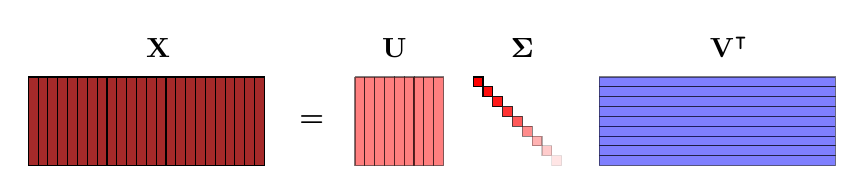
\begin{tikzpicture}[scale = 0.5]

  % draw line and angle
%  \draw 
%     pic [draw,angle radius=4mm,angle eccentricity=1.5, "$\theta$" font=\scriptsize] {angle=v2--v1--v3};
%\definecolor

\begin{scope}[xshift=7mm]
 

\draw [fill=Brown, opacity=1] (-16,4) -- (-15.75,4) -- (-15.75,1.75) -- (-16,1.75) -- (-16,4);
\draw [fill=Brown, opacity=1] (-15.75,4) -- (-15.5,4) -- (-15.5,1.75) -- (-15.75,1.75) -- (-15.75,4);

\draw [fill=Brown, opacity=1] (-15.5,4) -- (-15.25,4) -- (-15.25,1.75) -- (-15.5,1.75) -- (-15.5,4);
\draw [fill=Brown, opacity=1] (-15.25,4) -- (-15,4) -- (-15,1.75) -- (-15.25,1.75) -- (-15.25,4);
\draw [fill=Brown, opacity=1] (-15,4) -- (-14.75,4) -- (-14.75,1.75) -- (-15,1.75) -- (-15,4);
\draw [fill=Brown, opacity=1] (-14.75,4) -- (-14.5,4) -- (-14.5,1.75) -- (-14.75,1.75) -- (-14.75,4);
\draw [fill=Brown, opacity=1] (-14.5,4) -- (-14.25,4) -- (-14.25,1.75) -- (-14.5,1.75) -- (-14.5,4);
\draw [fill=Brown, opacity=1] (-14.25,4) -- (-14,4) -- (-14,1.75) -- (-14.25,1.75) -- (-14.25,4);
\draw [fill=Brown, opacity=1] (-14,4) -- (-13.75,4) -- (-13.75,1.75) -- (-14,1.75) -- (-14,4);
\draw [fill=Brown, opacity=1] (-13.75,4) -- (-13.5,4) -- (-13.5,1.75) -- (-13.75,1.75) -- (-13.75,4);
\draw [fill=Brown, opacity=1] (-13.5,4) -- (-13.25,4) -- (-13.25,1.75) -- (-13.5,1.75) -- (-13.5,4);
\draw [fill=Brown, opacity=1] (-13.25,4) -- (-13,4) -- (-13,1.75) -- (-13.25,1.75) -- (-13.25,4);
\draw [fill=Brown, opacity=1] (-13,4) -- (-12.75,4) -- (-12.75,1.75) -- (-13,1.75) -- (-13,4);

\draw [fill=Brown, opacity=1] (-12.75,4) -- (-12.5,4) -- (-12.5,1.75) -- (-12.75,1.75) -- (-12.75,4);
\draw [fill=Brown, opacity=1] (-12.5,4) -- (-12.25,4) -- (-12.25,1.75) -- (-12.5,1.75) -- (-12.5,4);
\draw [fill=Brown, opacity=1] (-12.25,4) -- (-12,4) -- (-12,1.75) -- (-12.25,1.75) -- (-12.25,4);
\draw [fill=Brown, opacity=1] (-12,4) -- (-11.75,4) -- (-11.75,1.75) -- (-12,1.75) -- (-12,4);

\draw [fill=Brown, opacity=1] (-11.75,4) -- (-11.5,4) -- (-11.5,1.75) -- (-11.75,1.75) -- (-11.75,4);
\draw [fill=Brown, opacity=1] (-11.5,4) -- (-11.25,4) -- (-11.25,1.75) -- (-11.5,1.75) -- (-11.5,4);
\draw [fill=Brown, opacity=1] (-11.25,4) -- (-11,4) -- (-11,1.75) -- (-11.25,1.75) -- (-11.25,4);
\draw [fill=Brown, opacity=1] (-11,4) -- (-10.75,4) -- (-10.75,1.75) -- (-11,1.75) -- (-11,4);
\draw [fill=Brown, opacity=1] (-10.75,4) -- (-10.5,4) -- (-10.5,1.75) -- (-10.75,1.75) -- (-10.75,4);
\draw [fill=Brown, opacity=1] (-10.5,4) -- (-10.25,4) -- (-10.25,1.75) -- (-10.5,1.75) -- (-10.5,4);
\draw [fill=Brown, opacity=1] (-10.25,4) -- (-10,4) -- (-10,1.75) -- (-10.25,1.75) -- (-10.25,4);


\end{scope}



\begin{scope}[xshift=0mm]
 
\draw [fill=red, opacity=0.5] (-7,4) -- (-6.75,4) -- (-6.75,1.75) -- (-7,1.75) -- (-7,4);
\draw [fill=red, opacity=0.5] (-6.75,4) -- (-6.5,4) -- (-6.5,1.75) -- (-6.75,1.75) -- (-6.75,4);
\draw [fill=red, opacity=0.5] (-6.5,4) -- (-6.25,4) -- (-6.25,1.75) -- (-6.5,1.75) -- (-6.5,4);

\draw [fill=red, opacity=0.5] (-6.25,4) -- (-6,4) -- (-6,1.75) -- (-6.25,1.75) -- (-6.25,4);
\draw [fill=red, opacity=0.5] (-6,4) -- (-5.75,4) -- (-5.75,1.75) -- (-6,1.75) -- (-6,4);
\draw [fill=red, opacity=0.5] (-5.75,4) -- (-5.5,4) -- (-5.5,1.75) -- (-5.75,1.75) -- (-5.75,4);
\draw [fill=red, opacity=0.5] (-5.5,4) -- (-5.25,4) -- (-5.25,1.75) -- (-5.5,1.75) -- (-5.5,4);

\draw [fill=red, opacity=0.5] (-5.25,4) -- (-5,4) -- (-5,1.75) -- (-5.25,1.75) -- (-5.25,4);
\draw [fill=red, opacity=0.5] (-5,4) -- (-4.75,4) -- (-4.75,1.75) -- (-5,1.75) -- (-5,4);
% \draw [fill=red, opacity=0.5] (-4.75,4) -- (-4.5,4) -- (-4.5,1.75) -- (-4.75,1.75) -- (-4.75,4);
% \draw [fill=red, opacity=0.5] (-4.5,4) -- (-4.25,4) -- (-4.25,1.75) -- (-4.5,1.75) -- (-4.5,4);


\end{scope}



\begin{scope}[xshift=-5mm]
 

\draw [fill=red, opacity=1] (-3.5,4) -- (-3.25,4) -- (-3.25,3.75) -- (-3.5,3.75) -- (-3.5,4);
\draw [fill=red, opacity=0.95] (-3.25,3.75) -- (-3,3.75) -- (-3,3.5) -- (-3.25,3.5) -- (-3.25,3.75);
\draw [fill=red, opacity=0.9] (-3,3.5) -- (-2.75,3.5) -- (-2.75,3.25) -- (-3,3.25) -- (-3,3.5);
\draw [fill=red, opacity=0.8] (-2.75,3.25) -- (-2.5,3.25) -- (-2.5,3) -- (-2.75,3) -- (-2.75,3.25);


\draw [fill=red, opacity=0.65] (-2.5,3) -- (-2.25,3) -- (-2.25,2.75) -- (-2.5,2.75) -- (-2.5,3);
\draw [fill=red, opacity=0.45] (-2.25,2.75) -- (-2,2.75) -- (-2,2.5) -- (-2.25,2.5) -- (-2.25,2.75);
\draw [fill=red, opacity=0.3] (-2,2.5) -- (-1.75,2.5) -- (-1.75,2.25) -- (-2,2.25) -- (-2,2.5);
\draw [fill=red, opacity=0.2] (-1.75,2.25) -- (-1.5,2.25) -- (-1.5,2) -- (-1.75,2) -- (-1.75,2.25);

\draw [fill=red, opacity=0.1] (-1.5,2) -- (-1.25,2) -- (-1.25,1.75) -- (-1.5,1.75) -- (-1.5,2);
\end{scope}


\begin{scope}[xshift=-18mm]
 
 
\draw [fill=blue, opacity=0.5] (7,3.75) -- (1,3.75) -- (1,4) -- (7,4) -- (7,3.75);
\draw [fill=blue, opacity=0.5] (7,3.5) -- (1,3.5) -- (1,3.75) -- (7,3.75) -- (7,3.5);
\draw [fill=blue, opacity=0.5] (7,3.25) -- (1,3.25) -- (1,3.5) -- (7,3.5) -- (7,3.25);
\draw [fill=blue, opacity=0.5] (7,3) -- (1,3) -- (1,3.25) -- (7,3.25) -- (7,3);
\draw [fill=blue, opacity=0.5] (7,2.75) -- (1,2.75) -- (1,3) -- (7,3) -- (7,2.75); 
\draw [fill=blue, opacity=0.5] (7,2.5) -- (1,2.5) -- (1,2.75) -- (7,2.75) -- (7,2.5);
\draw [fill=blue, opacity=0.5] (7,2.25) -- (1,2.25) -- (1,2.5) -- (7,2.5) -- (7,2.25);
\draw [fill=blue, opacity=0.5] (7,2) -- (1,2) -- (1,2.25) -- (7,2.25) -- (7,2);
\draw [fill=blue, opacity=0.5] (7,1.75) -- (1,1.75) -- (1,2) -- (7,2) -- (7,1.75);



\end{scope}




% \draw [fill=blue, opacity=0.5] (-16,3.75) -- (-10,3.75) -- (-10,4) -- (-16,4) -- (-16,3.75);
% \draw [fill=blue, opacity=0.5] (-16,3.5) -- (-10,3.5) -- (-10,3.75) -- (-16,3.75) -- (-16,3.5);
% \draw [fill=blue, opacity=0.5] (-16,3.25) -- (-10,3.25) -- (-10,3.5) -- (-16,3.5) -- (-16,3.25);
% \draw [fill=blue, opacity=0.5] (-16,3) -- (-10,3) -- (-10,3.25) -- (-16,3.25) -- (-16,3);
% \draw [fill=blue, opacity=0.5] (-16,2.75) -- (-10,2.75) -- (-10,3) -- (-16,3) -- (-16,2.75); 
% \draw [fill=blue, opacity=0.5] (-16,2.5) -- (-10,2.5) -- (-10,2.75) -- (-16,2.75) -- (-16,2.5);
% \draw [fill=blue, opacity=0.5] (-16,2.25) -- (-10,2.25) -- (-10,2.5) -- (-16,2.5) -- (-16,2.25);
% \draw [fill=blue, opacity=0.5] (-16,2) -- (-10,2) -- (-10,2.25) -- (-16,2.25) -- (-16,2);
% \draw [fill=blue, opacity=0.5] (-16,1.75) -- (-10,1.75) -- (-10,2) -- (-16,2) -- (-16,1.75);

\draw  (-12,4.25)  node [above] {$\bm{\mathrm{X}}$} ;
\draw  (-8.1,2.5)  node [above] {$\bm{=}$} ;

\draw  (-6,4.25)  node [above] {$\bm{\mathrm{U}}$} ;

\draw  (-2.75,4.25)  node [above] {$\bm{\mathrm{\Sigma}}$} ;

\draw  (2.5,4.25)  node [above] {$\bm{\mathrm{V}}^{\Tran}$} ;

%\draw  (-17.5,2.5)  node [above] {$\bm{V}^{\Tran}=$} ;


%\draw  (23,2)  node [above] {Complexity } ;

\end{tikzpicture}
}\\
%      \subfloat[Sampling $k$ columns according to VS and our DPP]{

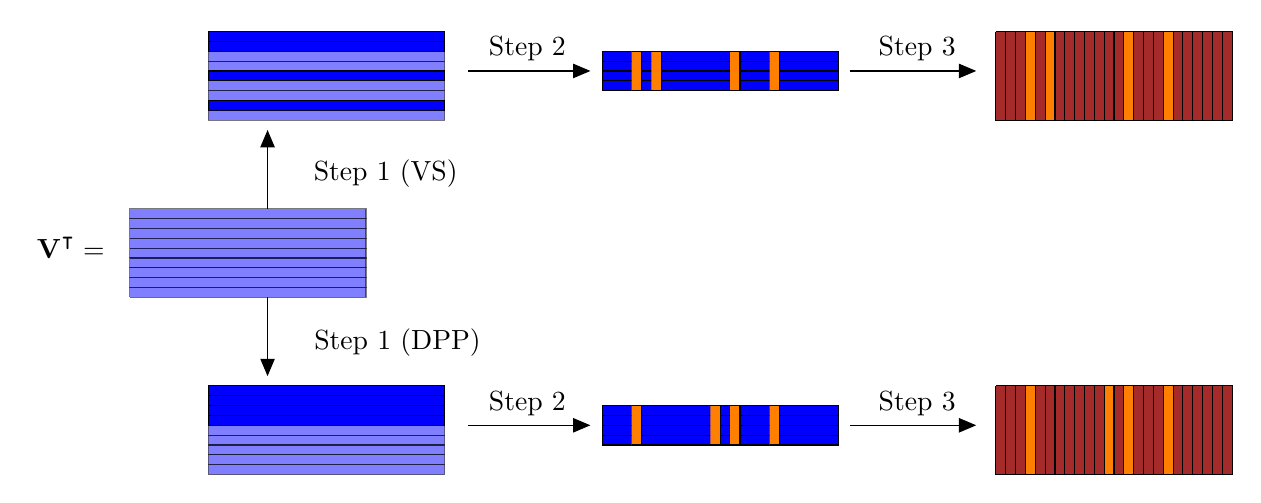
\begin{tikzpicture}[scale = 0.5]

  % draw line and angle
%  \draw
%     pic [draw,angle radius=4mm,angle eccentricity=1.5, "$\theta$" font=\scriptsize] {angle=v2--v1--v3};
\begin{scope}[yshift=-45mm]
\begin{scope}[xshift=-20mm]

\draw [fill=blue, opacity=0.5] (-16,3.75) -- (-10,3.75) -- (-10,4) -- (-16,4) -- (-16,3.75);
\draw [fill=blue, opacity=0.5] (-16,3.5) -- (-10,3.5) -- (-10,3.75) -- (-16,3.75) -- (-16,3.5);
\draw [fill=blue, opacity=0.5] (-16,3.25) -- (-10,3.25) -- (-10,3.5) -- (-16,3.5) -- (-16,3.25);
\draw [fill=blue, opacity=0.5] (-16,3) -- (-10,3) -- (-10,3.25) -- (-16,3.25) -- (-16,3);
\draw [fill=blue, opacity=0.5] (-16,2.75) -- (-10,2.75) -- (-10,3) -- (-16,3) -- (-16,2.75);
\draw [fill=blue, opacity=0.5] (-16,2.5) -- (-10,2.5) -- (-10,2.75) -- (-16,2.75) -- (-16,2.5);
\draw [fill=blue, opacity=0.5] (-16,2.25) -- (-10,2.25) -- (-10,2.5) -- (-16,2.5) -- (-16,2.25);
\draw [fill=blue, opacity=0.5] (-16,2) -- (-10,2) -- (-10,2.25) -- (-16,2.25) -- (-16,2);
\draw [fill=blue, opacity=0.5] (-16,1.75) -- (-10,1.75) -- (-10,2) -- (-16,2) -- (-16,1.75);


\draw  (-17.5,2.5)  node [above ] {$\bm{\mathrm{V}}^{\Tran} = $} ;

\draw  (-9.5,4.3)  node [above ] {Step 1 (VS)} ;

\draw [->] (-12.5,4) --  (-12.5,6);


\draw  (-9.2,0)  node [above ] {Step 1 (DPP)} ;

\draw [->] (-12.5,1.75) --  (-12.5,-0.25);

\end{scope}
\end{scope}





\begin{scope}[xshift=-120mm]


\draw [fill=blue, opacity=1] (-4,3.75) -- (2,3.75) -- (2,4) -- (-4,4) -- (-4,3.75);
\draw [fill=blue, opacity=1] (-4,3.5) -- (2,3.5) -- (2,3.75) -- (-4,3.75) -- (-4,3.5);
\draw [fill=blue, opacity=0.5] (-4,3.25) -- (2,3.25) -- (2,3.5) -- (-4,3.5) -- (-4,3.25);
\draw [fill=blue, opacity=0.5] (-4,3) -- (2,3) -- (2,3.25) -- (-4,3.25) -- (-4,3);
\draw [fill=blue, opacity=1] (-4,2.75) -- (2,2.75) -- (2,3) -- (-4,3) -- (-4,2.75);
\draw [fill=blue, opacity=0.5] (-4,2.5) -- (2,2.5) -- (2,2.75) -- (-4,2.75) -- (-4,2.5);
\draw [fill=blue, opacity=0.5] (-4,2.25) -- (2,2.25) -- (2,2.5) -- (-4,2.5) -- (-4,2.25);
\draw [fill=blue, opacity=1] (-4,2) -- (2,2) -- (2,2.25) -- (-4,2.25) -- (-4,2);
\draw [fill=blue, opacity=0.5] (-4,1.75) -- (2,1.75) -- (2,2) -- (-4,2) -- (-4,1.75);



\draw [->] (2.6,3) --  (4.1,3)  node [above] { Step 2 } --  (5.7,3);


\end{scope}


\begin{scope}[xshift=-120mm]
\begin{scope}[yshift=-90mm]


\draw [fill=blue, opacity=1] (-4,3.75) -- (2,3.75) -- (2,4) -- (-4,4) -- (-4,3.75);
\draw [fill=blue, opacity=1] (-4,3.5) -- (2,3.5) -- (2,3.75) -- (-4,3.75) -- (-4,3.5);
\draw [fill=blue, opacity=1] (-4,3.25) -- (2,3.25) -- (2,3.5) -- (-4,3.5) -- (-4,3.25);
\draw [fill=blue, opacity=1] (-4,3) -- (2,3) -- (2,3.25) -- (-4,3.25) -- (-4,3);
\draw [fill=blue, opacity=0.5] (-4,2.75) -- (2,2.75) -- (2,3) -- (-4,3) -- (-4,2.75);
\draw [fill=blue, opacity=0.5] (-4,2.5) -- (2,2.5) -- (2,2.75) -- (-4,2.75) -- (-4,2.5);
\draw [fill=blue, opacity=0.5] (-4,2.25) -- (2,2.25) -- (2,2.5) -- (-4,2.5) -- (-4,2.25);
\draw [fill=blue, opacity=0.5] (-4,2) -- (2,2) -- (2,2.25) -- (-4,2.25) -- (-4,2);
\draw [fill=blue, opacity=0.5] (-4,1.75) -- (2,1.75) -- (2,2) -- (-4,2) -- (-4,1.75);



\draw [->] (2.6,3) --  (4.1,3)  node [above] { Step 2 } --  (5.7,3);


\end{scope}
\end{scope}


\begin{scope}[xshift=-145mm]

\draw [fill=blue, opacity=1] (8.5,3.25) -- (14.5,3.25) -- (14.5,3.5) -- (8.5,3.5) -- (8.5,3.25);
\draw [fill=blue, opacity=1] (8.5,3) -- (14.5,3) -- (14.5,3.25) -- (8.5,3.25) -- (8.5,3);
\draw [fill=blue, opacity=1] (8.5,2.75) -- (14.5,2.75) -- (14.5,3) -- (8.5,3) -- (8.5,2.75);
\draw [fill=blue, opacity=1] (8.5,2.5) -- (14.5,2.5) -- (14.5,2.75) -- (8.5,2.75) -- (8.5,2.5);


\draw [fill=orange, opacity=1] (9.25,2.5) -- (9.25,2.5) -- (9.5,2.5) -- (9.5,3.5) -- (9.25,3.5);
\draw [fill=orange, opacity=1] (9.75,2.5) -- (9.75,2.5) -- (10,2.5) -- (10,3.5) -- (9.75,3.5);
\draw [fill=orange, opacity=1] (11.75,2.5) -- (11.75,2.5) -- (12,2.5) -- (12,3.5) -- (11.75,3.5);
\draw [fill=orange, opacity=1] (12.75,2.5) -- (12.75,2.5) -- (13,2.5) -- (13,3.5) -- (12.75,3.5);



\draw [->] (14.8,3) --  (16.5,3)  node [above] { Step 3 } --  (18,3);

\end{scope}

\begin{scope}[yshift=-90mm]
\begin{scope}[xshift=-145mm]

\draw [fill=blue, opacity=1] (8.5,3.25) -- (14.5,3.25) -- (14.5,3.5) -- (8.5,3.5) -- (8.5,3.25);
\draw [fill=blue, opacity=1] (8.5,3) -- (14.5,3) -- (14.5,3.25) -- (8.5,3.25) -- (8.5,3);
\draw [fill=blue, opacity=1] (8.5,2.75) -- (14.5,2.75) -- (14.5,3) -- (8.5,3) -- (8.5,2.75);
\draw [fill=blue, opacity=1] (8.5,2.5) -- (14.5,2.5) -- (14.5,2.75) -- (8.5,2.75) -- (8.5,2.5);


\draw [fill=orange, opacity=1] (9.25,2.5) -- (9.25,2.5) -- (9.5,2.5) -- (9.5,3.5) -- (9.25,3.5);
\draw [fill=orange, opacity=1] (11.25,2.5) -- (11.25,2.5) -- (11.5,2.5) -- (11.5,3.5) -- (11.25,3.5);
\draw [fill=orange, opacity=1] (11.75,2.5) -- (11.75,2.5) -- (12,2.5) -- (12,3.5) -- (11.75,3.5);
\draw [fill=orange, opacity=1] (12.75,2.5) -- (12.75,2.5) -- (13,2.5) -- (13,3.5) -- (12.75,3.5);



\draw [->] (14.8,3) --  (16.5,3)  node [above] { Step 3 } --  (18,3);

\end{scope}
\end{scope}

%\begin{scope}[yshift=-45mm]
\begin{scope}[xshift=200mm]
 

\draw [fill=Brown, opacity=1] (-16,4) -- (-15.75,4) -- (-15.75,1.75) -- (-16,1.75) -- (-16,4);
\draw [fill=Brown, opacity=1] (-15.75,4) -- (-15.5,4) -- (-15.5,1.75) -- (-15.75,1.75) -- (-15.75,4);

\draw [fill=Brown, opacity=1] (-15.5,4) -- (-15.25,4) -- (-15.25,1.75) -- (-15.5,1.75) -- (-15.5,4);
\draw [fill=orange, opacity=1] (-15.25,4) -- (-15,4) -- (-15,1.75) -- (-15.25,1.75) -- (-15.25,4);
\draw [fill=Brown, opacity=1] (-15,4) -- (-14.75,4) -- (-14.75,1.75) -- (-15,1.75) -- (-15,4);
\draw [fill=orange, opacity=1] (-14.75,4) -- (-14.5,4) -- (-14.5,1.75) -- (-14.75,1.75) -- (-14.75,4);
\draw [fill=Brown, opacity=1] (-14.5,4) -- (-14.25,4) -- (-14.25,1.75) -- (-14.5,1.75) -- (-14.5,4);
\draw [fill=Brown, opacity=1] (-14.25,4) -- (-14,4) -- (-14,1.75) -- (-14.25,1.75) -- (-14.25,4);
\draw [fill=Brown, opacity=1] (-14,4) -- (-13.75,4) -- (-13.75,1.75) -- (-14,1.75) -- (-14,4);
\draw [fill=Brown, opacity=1] (-13.75,4) -- (-13.5,4) -- (-13.5,1.75) -- (-13.75,1.75) -- (-13.75,4);
\draw [fill=Brown, opacity=1] (-13.5,4) -- (-13.25,4) -- (-13.25,1.75) -- (-13.5,1.75) -- (-13.5,4);
\draw [fill=Brown, opacity=1] (-13.25,4) -- (-13,4) -- (-13,1.75) -- (-13.25,1.75) -- (-13.25,4);
\draw [fill=Brown, opacity=1] (-13,4) -- (-12.75,4) -- (-12.75,1.75) -- (-13,1.75) -- (-13,4);

\draw [fill=orange, opacity=1] (-12.75,4) -- (-12.5,4) -- (-12.5,1.75) -- (-12.75,1.75) -- (-12.75,4);
\draw [fill=Brown, opacity=1] (-12.5,4) -- (-12.25,4) -- (-12.25,1.75) -- (-12.5,1.75) -- (-12.5,4);
\draw [fill=Brown, opacity=1] (-12.25,4) -- (-12,4) -- (-12,1.75) -- (-12.25,1.75) -- (-12.25,4);
\draw [fill=Brown, opacity=1] (-12,4) -- (-11.75,4) -- (-11.75,1.75) -- (-12,1.75) -- (-12,4);

\draw [fill=orange, opacity=1] (-11.75,4) -- (-11.5,4) -- (-11.5,1.75) -- (-11.75,1.75) -- (-11.75,4);
\draw [fill=Brown, opacity=1] (-11.5,4) -- (-11.25,4) -- (-11.25,1.75) -- (-11.5,1.75) -- (-11.5,4);
\draw [fill=Brown, opacity=1] (-11.25,4) -- (-11,4) -- (-11,1.75) -- (-11.25,1.75) -- (-11.25,4);
\draw [fill=Brown, opacity=1] (-11,4) -- (-10.75,4) -- (-10.75,1.75) -- (-11,1.75) -- (-11,4);
\draw [fill=Brown, opacity=1] (-10.75,4) -- (-10.5,4) -- (-10.5,1.75) -- (-10.75,1.75) -- (-10.75,4);
\draw [fill=Brown, opacity=1] (-10.5,4) -- (-10.25,4) -- (-10.25,1.75) -- (-10.5,1.75) -- (-10.5,4);
\draw [fill=Brown, opacity=1] (-10.25,4) -- (-10,4) -- (-10,1.75) -- (-10.25,1.75) -- (-10.25,4);


\end{scope}
%\end{scope}


\begin{scope}[yshift=-90mm]
\begin{scope}[xshift=200mm]
 

\draw [fill=Brown, opacity=1] (-16,4) -- (-15.75,4) -- (-15.75,1.75) -- (-16,1.75) -- (-16,4);
\draw [fill=Brown, opacity=1] (-15.75,4) -- (-15.5,4) -- (-15.5,1.75) -- (-15.75,1.75) -- (-15.75,4);

\draw [fill=Brown, opacity=1] (-15.5,4) -- (-15.25,4) -- (-15.25,1.75) -- (-15.5,1.75) -- (-15.5,4);
\draw [fill=orange, opacity=1] (-15.25,4) -- (-15,4) -- (-15,1.75) -- (-15.25,1.75) -- (-15.25,4);
\draw [fill=Brown, opacity=1] (-15,4) -- (-14.75,4) -- (-14.75,1.75) -- (-15,1.75) -- (-15,4);
\draw [fill=Brown, opacity=1] (-14.75,4) -- (-14.5,4) -- (-14.5,1.75) -- (-14.75,1.75) -- (-14.75,4);
\draw [fill=Brown, opacity=1] (-14.5,4) -- (-14.25,4) -- (-14.25,1.75) -- (-14.5,1.75) -- (-14.5,4);
\draw [fill=Brown, opacity=1] (-14.25,4) -- (-14,4) -- (-14,1.75) -- (-14.25,1.75) -- (-14.25,4);
\draw [fill=Brown, opacity=1] (-14,4) -- (-13.75,4) -- (-13.75,1.75) -- (-14,1.75) -- (-14,4);
\draw [fill=Brown, opacity=1] (-13.75,4) -- (-13.5,4) -- (-13.5,1.75) -- (-13.75,1.75) -- (-13.75,4);
\draw [fill=Brown, opacity=1] (-13.5,4) -- (-13.25,4) -- (-13.25,1.75) -- (-13.5,1.75) -- (-13.5,4);
\draw [fill=orange, opacity=1] (-13.25,4) -- (-13,4) -- (-13,1.75) -- (-13.25,1.75) -- (-13.25,4);
\draw [fill=Brown, opacity=1] (-13,4) -- (-12.75,4) -- (-12.75,1.75) -- (-13,1.75) -- (-13,4);

\draw [fill=orange, opacity=1] (-12.75,4) -- (-12.5,4) -- (-12.5,1.75) -- (-12.75,1.75) -- (-12.75,4);
\draw [fill=Brown, opacity=1] (-12.5,4) -- (-12.25,4) -- (-12.25,1.75) -- (-12.5,1.75) -- (-12.5,4);
\draw [fill=Brown, opacity=1] (-12.25,4) -- (-12,4) -- (-12,1.75) -- (-12.25,1.75) -- (-12.25,4);
\draw [fill=Brown, opacity=1] (-12,4) -- (-11.75,4) -- (-11.75,1.75) -- (-12,1.75) -- (-12,4);

\draw [fill=orange, opacity=1] (-11.75,4) -- (-11.5,4) -- (-11.5,1.75) -- (-11.75,1.75) -- (-11.75,4);
\draw [fill=Brown, opacity=1] (-11.5,4) -- (-11.25,4) -- (-11.25,1.75) -- (-11.5,1.75) -- (-11.5,4);
\draw [fill=Brown, opacity=1] (-11.25,4) -- (-11,4) -- (-11,1.75) -- (-11.25,1.75) -- (-11.25,4);
\draw [fill=Brown, opacity=1] (-11,4) -- (-10.75,4) -- (-10.75,1.75) -- (-11,1.75) -- (-11,4);
\draw [fill=Brown, opacity=1] (-10.75,4) -- (-10.5,4) -- (-10.5,1.75) -- (-10.75,1.75) -- (-10.75,4);
\draw [fill=Brown, opacity=1] (-10.5,4) -- (-10.25,4) -- (-10.25,1.75) -- (-10.5,1.75) -- (-10.5,4);
\draw [fill=Brown, opacity=1] (-10.25,4) -- (-10,4) -- (-10,1.75) -- (-10.25,1.75) -- (-10.25,4);


\end{scope}
\end{scope}

% \begin{scope}[xshift=-50mm]





% \end{scope}

%\draw  (23,2)  node [above] {Complexity } ;

\end{tikzpicture}
}
%   %  \subfloat[]{

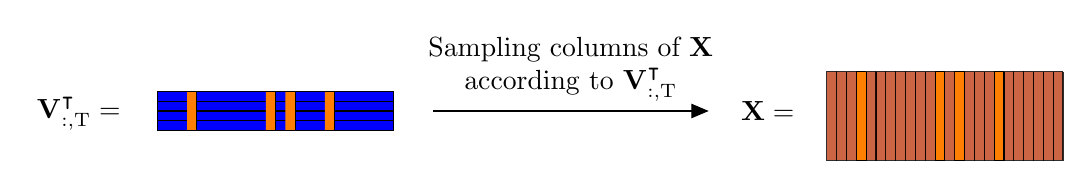
\begin{tikzpicture}[scale = 0.5]

  % draw line and angle
%  \draw 
%     pic [draw,angle radius=4mm,angle eccentricity=1.5, "$\theta$" font=\scriptsize] {angle=v2--v1--v3};

\begin{scope}[xshift=-65mm]



\draw [fill=blue, opacity=1] (0.5,3.25) -- (6.5,3.25) -- (6.5,3.5) -- (0.5,3.5) -- (0.5,3.25);
\draw [fill=blue, opacity=1] (0.5,3) -- (6.5,3) -- (6.5,3.25) -- (0.5,3.25) -- (0.5,3);
\draw [fill=blue, opacity=1] (0.5,2.75) -- (6.5,2.75) -- (6.5,3) -- (0.5,3) -- (0.5,2.75);
\draw [fill=blue, opacity=1] (0.5,2.5) -- (6.5,2.5) -- (6.5,2.75) -- (0.5,2.75) -- (0.5,2.5);


\draw [fill=orange, opacity=1] (1.25,2.5) -- (1.25,2.5) -- (1.5,2.5) -- (1.5,3.5) -- (1.25,3.5);
\draw [fill=orange, opacity=1] (3.25,2.5) -- (3.25,2.5) -- (3.5,2.5) -- (3.5,3.5) -- (3.25,3.5);
\draw [fill=orange, opacity=1] (3.75,2.5) -- (3.75,2.5) -- (4,2.5) -- (4,3.5) -- (3.75,3.5);
\draw [fill=orange, opacity=1] (4.75,2.5) -- (4.75,2.5) -- (5,2.5) -- (5,3.5) -- (4.75,3.5);


 \draw  (-1.5,2.25)  node [above] {$\bm{\mathrm{V}}_{:,\mathrm{T}}^{\Tran}=$} ;
\end{scope}

\begin{scope}[xshift=10mm]


\draw [fill=Bittersweet, opacity=0.8] (16,4) -- (15.75,4) -- (15.75,1.75) -- (16,1.75) -- (16,4);
\draw [fill=Bittersweet, opacity=0.8] (15.75,4) -- (15.5,4) -- (15.5,1.75) -- (15.75,1.75) -- (15.75,4);

\draw [fill=Bittersweet, opacity=0.8] (15.5,4) -- (15.25,4) -- (15.25,1.75) -- (15.5,1.75) -- (15.5,4);
\draw [fill=Bittersweet, opacity=0.8] (15.25,4) -- (15,4) -- (15,1.75) -- (15.25,1.75) -- (15.25,4);
\draw [fill=Bittersweet, opacity=0.8] (15,4) -- (14.75,4) -- (14.75,1.75) -- (15,1.75) -- (15,4);
\draw [fill=Bittersweet, opacity=0.8] (14.75,4) -- (14.5,4) -- (14.5,1.75) -- (14.75,1.75) -- (14.75,4);
\draw [fill=orange, opacity=1] (14.5,4) -- (14.25,4) -- (14.25,1.75) -- (14.5,1.75) -- (14.5,4);
\draw [fill=Bittersweet, opacity=0.8] (14.25,4) -- (14,4) -- (14,1.75) -- (14.25,1.75) -- (14.25,4);
\draw [fill=Bittersweet, opacity=0.8] (14,4) -- (13.75,4) -- (13.75,1.75) -- (14,1.75) -- (14,4);
\draw [fill=Bittersweet, opacity=0.8] (13.75,4) -- (13.5,4) -- (13.5,1.75) -- (13.75,1.75) -- (13.75,4);
\draw [fill=orange, opacity=1] (13.5,4) -- (13.25,4) -- (13.25,1.75) -- (13.5,1.75) -- (13.5,4);
\draw [fill=Bittersweet, opacity=0.8] (13.25,4) -- (13,4) -- (13,1.75) -- (13.25,1.75) -- (13.25,4);
\draw [fill=orange, opacity=1] (13,4) -- (12.75,4) -- (12.75,1.75) -- (13,1.75) -- (13,4);

\draw [fill=Bittersweet, opacity=0.8] (12.75,4) -- (12.5,4) -- (12.5,1.75) -- (12.75,1.75) -- (12.75,4);
\draw [fill=Bittersweet, opacity=0.8] (12.5,4) -- (12.25,4) -- (12.25,1.75) -- (12.5,1.75) -- (12.5,4);
\draw [fill=Bittersweet, opacity=0.8] (12.25,4) -- (12,4) -- (12,1.75) -- (12.25,1.75) -- (12.25,4);
\draw [fill=Bittersweet, opacity=0.8] (12,4) -- (11.75,4) -- (11.75,1.75) -- (12,1.75) -- (12,4);

\draw [fill=Bittersweet, opacity=0.8] (11.75,4) -- (11.5,4) -- (11.5,1.75) -- (11.75,1.75) -- (11.75,4);
\draw [fill=Bittersweet, opacity=0.8] (11.5,4) -- (11.25,4) -- (11.25,1.75) -- (11.5,1.75) -- (11.5,4);
\draw [fill=Bittersweet, opacity=0.8] (11.25,4) -- (11,4) -- (11,1.75) -- (11.25,1.75) -- (11.25,4);
\draw [fill=orange, opacity=1] (11,4) -- (10.75,4) -- (10.75,1.75) -- (11,1.75) -- (11,4);
\draw [fill=Bittersweet, opacity=0.8] (10.75,4) -- (10.5,4) -- (10.5,1.75) -- (10.75,1.75) -- (10.75,4);
\draw [fill=Bittersweet, opacity=0.8] (10.5,4) -- (10.25,4) -- (10.25,1.75) -- (10.5,1.75) -- (10.5,4);
\draw [fill=Bittersweet, opacity=0.8] (10.25,4) -- (10,4) -- (10,1.75) -- (10.25,1.75) -- (10.25,4);


\draw  (8.5,2.5)  node [above] {$\bm{\mathrm{X}} = $} ;
\end{scope}


\draw [->] (1,3) --  (4.5,3)  node [above] {} --  (8,3);

\draw  (4.5,3)  node [above , align=center] {Sampling columns of $\bm{\mathrm{X}}$\\ according to $\bm{\mathrm{V}}_{:,\mathrm{T}}^{\Tran}$} ;



% \draw [->] (-9.5,3) --  (-7.5,3)  node [above] { $\Prb(T)$} --  (-5,3);

% \draw [->] (3,3) --  (5,3)  node [above] { $\Prb(S|T)$} --  (7.5,3);


% \draw  (-7.5,4.25)  node [above] {Step 1} ;

% \draw  (5,4.25)  node [above] {Step 2} ;

%\draw  (23,2)  node [above] {Complexity } ;

\end{tikzpicture}
}\\
%     %\caption{DPP sampling algorithm
%     %\label{f:dpp_sampling_algorithm}
%     %}
% %    \subfloat[]{

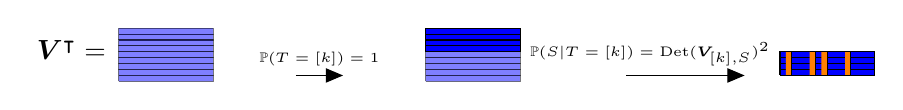
\begin{tikzpicture}[scale = 0.3]

  % draw line and angle
%  \draw 
%     pic [draw,angle radius=4mm,angle eccentricity=1.5, "$\theta$" font=\scriptsize] {angle=v2--v1--v3};

 



 

\draw [fill=blue, opacity=0.5] (-15,3.75) -- (-11,3.75) -- (-11,4) -- (-15,4) -- (-15,3.75);
\draw [fill=blue, opacity=0.5] (-15,3.5) -- (-11,3.5) -- (-11,3.75) -- (-15,3.75) -- (-15,3.5);
\draw [fill=blue, opacity=0.5] (-15,3.25) -- (-11,3.25) -- (-11,3.5) -- (-15,3.5) -- (-15,3.25);
\draw [fill=blue, opacity=0.5] (-15,3) -- (-11,3) -- (-11,3.25) -- (-15,3.25) -- (-15,3);
\draw [fill=blue, opacity=0.5] (-15,2.75) -- (-11,2.75) -- (-11,3) -- (-15,3) -- (-15,2.75); 
\draw [fill=blue, opacity=0.5] (-15,2.5) -- (-11,2.5) -- (-11,2.75) -- (-15,2.75) -- (-15,2.5);
\draw [fill=blue, opacity=0.5] (-15,2.25) -- (-11,2.25) -- (-11,2.5) -- (-15,2.5) -- (-15,2.25);
\draw [fill=blue, opacity=0.5] (-15,2) -- (-11,2) -- (-11,2.25) -- (-15,2.25) -- (-15,2);
\draw [fill=blue, opacity=0.5] (-15,1.75) -- (-11,1.75) -- (-11,2) -- (-15,2) -- (-15,1.75);



\draw [fill=blue, opacity=1] (-2,3.75) -- (2,3.75) -- (2,4) -- (-2,4) -- (-2,3.75);
\draw [fill=blue, opacity=1] (-2,3.5) -- (2,3.5) -- (2,3.75) -- (-2,3.75) -- (-2,3.5);
\draw [fill=blue, opacity=1] (-2,3.25) -- (2,3.25) -- (2,3.5) -- (-2,3.5) -- (-2,3.25);
\draw [fill=blue, opacity=1] (-2,3) -- (2,3) -- (2,3.25) -- (-2,3.25) -- (-2,3);
\draw [fill=blue, opacity=0.5] (-2,2.75) -- (2,2.75) -- (2,3) -- (-2,3) -- (-2,2.75); 
\draw [fill=blue, opacity=0.5] (-2,2.5) -- (2,2.5) -- (2,2.75) -- (-2,2.75) -- (-2,2.5);
\draw [fill=blue, opacity=0.5] (-2,2.25) -- (2,2.25) -- (2,2.5) -- (-2,2.5) -- (-2,2.25);
\draw [fill=blue, opacity=0.5] (-2,2) -- (2,2) -- (2,2.25) -- (-2,2.25) -- (-2,2);
\draw [fill=blue, opacity=0.5] (-2,1.75) -- (2,1.75) -- (2,2) -- (-2,2) -- (-2,1.75);





\draw [fill=blue, opacity=1] (13,2.75) -- (17,2.75) -- (17,3) -- (13,3) -- (13,2.75);
\draw [fill=blue, opacity=1] (13,2.5) -- (17,2.5) -- (17,2.75) -- (13,2.75) -- (13,2.5);
\draw [fill=blue, opacity=1] (13,2.25) -- (17,2.25) -- (17,2.5) -- (13,2.5) -- (13,2.25);
\draw [fill=blue, opacity=1] (13,2) -- (17,2) -- (17,2.25) -- (13,2.25) -- (13,2);


\draw [fill=orange, opacity=1] (13.25,2) -- (13.25,2) -- (13.5,2) -- (13.5,3) -- (13.25,3);
\draw [fill=orange, opacity=1] (14.25,2) -- (14.25,2) -- (14.5,2) -- (14.5,3) -- (14.25,3);
\draw [fill=orange, opacity=1] (14.75,2) -- (14.75,2) -- (15,2) -- (15,3) -- (14.75,3);
\draw [fill=orange, opacity=1] (15.75,2) -- (15.75,2) -- (16,2) -- (16,3) -- (15.75,3);



\draw [->] (-7.5,2) --  (-6.5,2)  node [above] {\tiny $\Prb(T = [k]) = 1$} --  (-5.5,2);

\draw [->] (6.5,2) --  (7.5,2)  node [above] {\tiny $\Prb(S|T = [k]) = \Det (\bm{V}_{[k],S})^{2}$} --  (11.5,2);

\draw  (-17,2.25)  node [above] {$\bm{V}^{\Tran}=$} ;

\end{tikzpicture}
}\\
% %\subfloat[]{

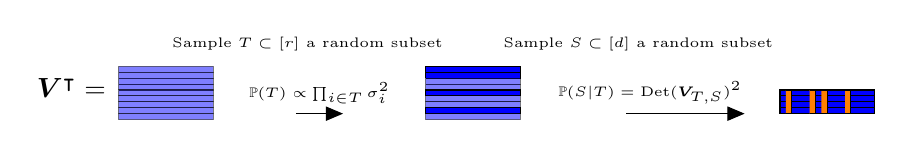
\begin{tikzpicture}[scale = 0.3]

  % draw line and angle
%  \draw 
%     pic [draw,angle radius=4mm,angle eccentricity=1.5, "$\theta$" font=\scriptsize] {angle=v2--v1--v3};

 

\draw [fill=blue, opacity=0.5] (-15,3.75) -- (-11,3.75) -- (-11,4) -- (-15,4) -- (-15,3.75);
\draw [fill=blue, opacity=0.5] (-15,3.5) -- (-11,3.5) -- (-11,3.75) -- (-15,3.75) -- (-15,3.5);
\draw [fill=blue, opacity=0.5] (-15,3.25) -- (-11,3.25) -- (-11,3.5) -- (-15,3.5) -- (-15,3.25);
\draw [fill=blue, opacity=0.5] (-15,3) -- (-11,3) -- (-11,3.25) -- (-15,3.25) -- (-15,3);
\draw [fill=blue, opacity=0.5] (-15,2.75) -- (-11,2.75) -- (-11,3) -- (-15,3) -- (-15,2.75); 
\draw [fill=blue, opacity=0.5] (-15,2.5) -- (-11,2.5) -- (-11,2.75) -- (-15,2.75) -- (-15,2.5);
\draw [fill=blue, opacity=0.5] (-15,2.25) -- (-11,2.25) -- (-11,2.5) -- (-15,2.5) -- (-15,2.25);
\draw [fill=blue, opacity=0.5] (-15,2) -- (-11,2) -- (-11,2.25) -- (-15,2.25) -- (-15,2);
\draw [fill=blue, opacity=0.5] (-15,1.75) -- (-11,1.75) -- (-11,2) -- (-15,2) -- (-15,1.75);



\draw [fill=blue, opacity=1] (-2,3.75) -- (2,3.75) -- (2,4) -- (-2,4) -- (-2,3.75);
\draw [fill=blue, opacity=1] (-2,3.5) -- (2,3.5) -- (2,3.75) -- (-2,3.75) -- (-2,3.5);
\draw [fill=blue, opacity=0.5] (-2,3.25) -- (2,3.25) -- (2,3.5) -- (-2,3.5) -- (-2,3.25);
\draw [fill=blue, opacity=0.5] (-2,3) -- (2,3) -- (2,3.25) -- (-2,3.25) -- (-2,3);
\draw [fill=blue, opacity=1] (-2,2.75) -- (2,2.75) -- (2,3) -- (-2,3) -- (-2,2.75); 
\draw [fill=blue, opacity=0.5] (-2,2.5) -- (2,2.5) -- (2,2.75) -- (-2,2.75) -- (-2,2.5);
\draw [fill=blue, opacity=0.5] (-2,2.25) -- (2,2.25) -- (2,2.5) -- (-2,2.5) -- (-2,2.25);
\draw [fill=blue, opacity=1] (-2,2) -- (2,2) -- (2,2.25) -- (-2,2.25) -- (-2,2);
\draw [fill=blue, opacity=0.5] (-2,1.75) -- (2,1.75) -- (2,2) -- (-2,2) -- (-2,1.75);





\draw [fill=blue, opacity=1] (13,2.75) -- (17,2.75) -- (17,3) -- (13,3) -- (13,2.75);
\draw [fill=blue, opacity=1] (13,2.5) -- (17,2.5) -- (17,2.75) -- (13,2.75) -- (13,2.5);
\draw [fill=blue, opacity=1] (13,2.25) -- (17,2.25) -- (17,2.5) -- (13,2.5) -- (13,2.25);
\draw [fill=blue, opacity=1] (13,2) -- (17,2) -- (17,2.25) -- (13,2.25) -- (13,2);


\draw [fill=orange, opacity=1] (13.25,2) -- (13.25,2) -- (13.5,2) -- (13.5,3) -- (13.25,3);
\draw [fill=orange, opacity=1] (14.25,2) -- (14.25,2) -- (14.5,2) -- (14.5,3) -- (14.25,3);
\draw [fill=orange, opacity=1] (14.75,2) -- (14.75,2) -- (15,2) -- (15,3) -- (14.75,3);
\draw [fill=orange, opacity=1] (15.75,2) -- (15.75,2) -- (16,2) -- (16,3) -- (15.75,3);



\draw [->] (-7.5,2) --  (-6.5,2)  node [above] {\tiny $\Prb(T) \propto \prod_{i \in T} \sigma_{i}^{2}$} --  (-5.5,2);

\draw [->] (6.5,2) --  (7.5,2)  node [above] {\tiny $\Prb(S|T) = \Det (\bm{V}_{T,S})^{2}$} --  (11.5,2);

\draw  (-17,2.25)  node [above] {$\bm{V}^{\Tran}=$} ;

\draw  (-7,4.25)  node [above] {\tiny Sample $T \subset [r]$ a random subset} ;

\draw  (7,4.25)  node [above] {\tiny Sample $S \subset [d]$ a random subset} ;

%\draw  (23,2)  node [above] {Complexity } ;

\end{tikzpicture}
}
%     %\caption{Volume sampling algorithm
%     %label{f:volume_sampling_algorithm}
%     %}
%     \caption{A graphical depiction of the sampling algorithms for volume sampling (VS) and the DPP with marginal kernel $\bm{V}^{}_{k}\bm{V}_{k}^{\Tran}$. (a) Both algorithms start with an SVD. (b) In Step 1, VS randomly selects $k$ rows of $\bm V^{\Tran}$, while our DPP always picks the first $k$ rows. Step 2 is the same for both algorithms: jointly sample $k$ columns of the subsampled $\bm V^{\Tran}$, proportionally to their squared volume. Finally, Step 3 is simply the extraction of the corresponding columns of $\bm X$.
%     %The common steps on the sampling algorithm for DPPs and volume sampling. Step 1: sample a random subset of right eigenvectors $T \subseteq [r]$with probability $\Prb(T)$. Step 2: sample a random subset of columns indices $S \subseteq [d]$ with probability $\Prb(S|T)$.
%     \label{f:sampling}
%     }
% \end{figure}

% \begin{table}
% \centering
%  \begin{tabular}{| c| c| c|}
%  \hline
%   - & Step 1 & Step 2\\
%  \hline
%  Projection DPP & $\Prb(T=[k]) = 1$ & $\Prb(S|T) = \Det (\bm{V}_{S,[k]})^{2}$\\
%  \hline
%  DPP & $\Prb(t \in T) = \lambda_{t}$ & $\Prb(S|T) = \Det (\bm{V}_{S,T})^{2}$\\
%  \hline
%  Volume sampling & $\Prb(T) \propto \prod_{i \in T} \sigma_{i}^{2}$ & $\Prb(S|T) = \Det (\bm{V}_{S,T})^{2}$\\
%  \hline
% \end{tabular}
% \caption{Differences in sampling schemes between projection DPP, DPP and volume sampling.}
% \end{table}

A fundamental example of $k$-DPPs is volume sampling, as defined in Section \ref{subsec:volume_sampling}. Its kernel is the Gram matrix of the data $\bm{L} = \bm{X}^{\Tran}\bm{X}$. In general, $\bm{L}$ is not an orthogonal projection matrix, so that volume sampling is not a DPP. In particular, draws from volume sampling have fixed cardinality, and thus cannot be written as a sum of non trivial Bernoulli random variables.

\subsection{Motivations for column subset selection using projection DPPs}
Volume sampling has been successfully used for column subset selection, see Section~\ref{subsec:volume_sampling}. Our motivation to investigate projection DPPs instead of volume sampling is twofold.

Following \eqref{eq:volume_sampling_as_mixture_equation}, volume sampling can be seen as a mixture of projection DPPs indexed by $T\subseteq [d], \vert T\vert=k$, with marginal kernels $\bm{K}_{T} = \bm{V}^{}_{:,T}\bm{V}^{\Tran}_{:,T}$ and mixture weights $\mu_{T} \propto \prod_{i \in T} \sigma_{i}^{2}$. The component with the highest weight thus corresponds to the $k$ largest singular values, that is, the projection DPP with marginal kernel
$\bm K:=\bm{V}^{}_{k}\bm{V}_{k}^{\Tran}$. This paper is about column subset selection using precisely this DPP. Alternately, we could motivate the study of this DPP by remarking that its marginals $\Prb({i}\subseteq Y)$ are the $k$-leverage scores introduced in Section~\ref{subsec:k-lvs_sampling}. Since $\bm K$ is symmetric, this DPP can be seen as a repulsive generalization of leverage score sampling.

Finally, we recap the difference between volume sampling and the DPP with kernel $\bm K$ with a graphical depiction in Figure~\ref{f:sampling} of the two procedures to sample from them that we introduced in Section~\ref{subsec:sampling_from_a_dpp}. Figure~\ref{f:sampling} is another illustration of the decomposition of volume sampling as a mixture of projection DPPs.
% \subsubsection{The projection DPPs}
% \subsubsection{The intuitions}
\paragraph{Principal angles between subspaces}
This section surveys the notion of principal angles between subspaces, see \cite[Section 6.4.3]{GoVa96} for details.
\begin{definition}
  \label{d:angles}
Let $\mathcal{P},\mathcal{Q}$ be two subspaces in $\mathbb{R}^{d}$. Let $p= \dim\mathcal{P}$ and $q = \dim\mathcal{Q}$ and assume that $q \leq p$. To define the vector of principal angles $\bm{\theta} \in [0,\pi/2]^{q}$ between $\mathcal{P}$ and $\mathcal{Q}$, let
\begin{equation}\label{eq:max_def_principal_angle_1}
 \cos(\theta_{1}) = \max \left\{ \frac{\bm{x}^{T}\bm{y}}{\|\bm{x}\|\|\bm{y}\|}; \quad \bm{x} \in \mathcal{P}, \bm{y} \in \mathcal{Q} \right\}
\end{equation}
be the cosine of the smallest angle between a vector of $\mathcal{P}$ and a vector of $\mathcal{Q}$, and let $(\bm{x}_{1},\bm{y}_{1}) \in \mathcal{P}\times \mathcal{Q}$ be a pair of vectors realizing the maximum. For $i \in [2,q]$, define successively
\begin{equation}\label{eq:max_def_principal_angles}
 \cos(\theta_{i}) = \max \left\{\frac{\bm{x}^{T}\bm{y}}{\|\bm{x}\|\|\bm{y}\|}; \quad \bm{x} \in \mathcal{P}, \bm{y} \in \mathcal{Q}; \bm{x} \perp \bm{x}_{j}, \bm{y} \perp \bm{y}_{j}\:, \forall j \in [1:i-1] \right\}
\end{equation}
and denote $(\bm{x}_{i},\bm{y}_{i}) \in \mathcal{P}\times\mathcal{Q}$ such that $\cos(\theta_{i}) = \bm{x}_{i}^{\Tran}\bm{y}_{i} \:$.
\end{definition}
Note that although the so-called principal vectors $(\bm{x}_{i},\bm{y}_{i})_{i \in [q]}$
are not uniquely defined by \eqref{eq:max_def_principal_angle_1} and \eqref{eq:max_def_principal_angles}, the principal angles $\bm{\theta}$ are uniquely defined, see \citep{BjGo73}. The following result confirms this, while also providing a way to compute $\bm{\theta}$.
\begin{proposition}[\citealp{BjGo73}, \citealp{Ben92}]
  \label{principal_angles_theorem_1}
Let $\mathcal{P}$ and $\mathcal{Q}$ and $\bm{\theta}$ be as in Definition~\ref{d:angles}. Let $\bm{P} \in \mathbb{R}^{d \times p}$, $\bm{Q} \in \mathbb{R}^{d \times q}$ be two orthogonal matrices, whose columns are orthonormal bases of $\mathcal{P}$ and $\mathcal{Q}$, respectively. Then
\begin{equation}
 \forall i \in [q], \quad \cos(\theta_{i}) =\sigma_i(\bm{Q}^{\Tran}\bm{P}).
\end{equation}
% Furthermore, we have $\lambda_{k} = ... = \lambda_{k-n} = 0 < \lambda_{k-n-1} \Leftrightarrow dim \mathcal{P} \cap \mathcal{Q} = n$
In particular
\begin{equation}\label{principal_angles_formula}
\Vol_{q}^{2}(\bm{Q}^{\Tran}\bm{P}) = \prod\limits_{i \in [q]} \cos^{2}(\theta_{i}).
\end{equation}
\end{proposition}
%\ab{a sentence on the relationship between cos and vol}
An important case for our work arises when $q=k$, $\bm{Q}=\bm{V} \in \mathbb{R}^{d \times k}$, and $\bm{P}=\bm{S}\in \mathbb{R}^{d \times k}$ is a sampling matrix. The left-hand side of \eqref{principal_angles_formula} then equals $\Det(\bm{V}_{:,S})^2$.

% Thus $\Vol_{q}^{2}(\bm{Q}^{\Tran}\bm{P})$ depends uniquely on the principal angles $((\theta_{i})_{i \in [1:q]})$ between the subspaces $\mathcal{P}$ and $\mathcal{Q}$. Therefore $\Vol_{q}^{2}(\bm{Q}^{\Tran}\bm{P})$ is independent of the choice of $\bm{P}$ and $\bm{Q}$.
% We define:
% \begin{equation}
%     \cos(\mathcal{P},\mathcal{Q}) =  \prod\limits_{i \in [1:q]} \cos(\theta_{i})
% \end{equation}
% and note that we have
% \begin{equation}
% \Vol_{q}(\bm{Q}^{\Tran}\bm{P}) = |\cos(\mathcal{P},\mathcal{Q})| \: .
% \end{equation}
% \begin{example}
% In the case of $d = 3$ and $p = q = k = 2$. We have $dim \mathcal{P} \cap \mathcal{Q} = 1$ then $\theta_{1} = 0$ and $\theta_{2}$ is the maximal angle between $\mathcal{P}$ and $\mathcal{Q}$.
% \end{example}


%\begin{figure}[!ht]
%    \centering
%    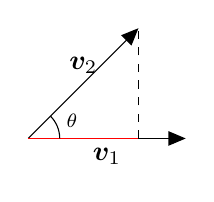
\begin{tikzpicture}
  \coordinate (v1) at (0,0);
  \coordinate (v2) at (2,0);
  \coordinate (v3) at (1.4,1.4);
  \coordinate (v4) at (1.4,0);
  % add coordinate at the extension of the line from v1 to v2
  \coordinate (v2-2) at ($(v1)!1.2!(v2)$); 

  \draw[->] (v1) -- node[below] {$\bm{v}_{1}$} (v2);
  \draw[->] (v1) -- node[above] {$\bm{v}_{2}$} (v3);
  \draw[red,-] (v1) -- node[below] {} (v4);
  \draw[dashed] (v4) -- node[below] {} (v3);

  % draw line and angle
  \draw 
     pic [draw,angle radius=4mm,angle eccentricity=1.5, "$\theta$" font=\scriptsize] {angle=v2--v1--v3};

\end{tikzpicture}

%    \caption{The shadow in red is equal to $cos(\theta) = \bm{v}_{1}^{T}\bm{v}_{2}$ ($\|\bm{v}_{1}\|_{2}= \|\bm{v}_{2}\|_{2} = 1$). The equality \ref{principal_angles_formula} is a generalization of this formula for multiple vectors.
%    \label{f:angles_between_subspaces}
%    }
%\end{figure}

\subsubsection{The Cosine Sine decomposition}
The Cosine Sine (CS) decomposition is useful for the study of the relative position of two subspaces. It generalizes the notion of cosine, sine and tangent to subspaces. The tangent of principal angles between subspaces were first mentioned in \citealp{ZhKn13}.
\begin{proposition}[\citealp{GoVa96}]
Let $q,d \in \mathbb{N}$ and $\bm{Q} =
\left[
\begin{array}{c}
\bm{Q}_{1}  \\
\hline
\bm{Q}_{2}
\end{array}
\right]
$ be a $d\times q$ orthogonal matrix, where $\bm{Q}_{1} \in \mathbb{R}^{q \times q}$ and $\bm{Q}_{2} \in \mathbb{R}^{(d-q)\times q}$. Assume that $\bm{Q}_{1}$ is non singular, then there exist orthogonal matrices $\bm{Y}\in\mathbb{R}^{d \times q}$ and
\begin{equation}
 \bm{W} =
\left[
\begin{array}{c|c}
\bm{W}_{1} & \bm{0} \\
\hline
\bm{0} & \bm{W}_{2}
\end{array}
\right]~\in~\mathbb{R}^{d \times d},
\end{equation}
%and $\bm{Y}~\in~\mathbb{R}^{d \times q}$,
and a matrix
\begin{equation}
\bm{\Sigma}~=~\left[
\begin{array}{c}
\Cosmatrix \\
\hline
\Sinmatrix \\
\hline
\bm{0}_{q',q}
\end{array}
\right] \in \mathbb{R}^{d \times q},
\end{equation}
where $q' = \max(0,d-2q)$, such that
\begin{equation}
    \bm{Q} = \bm{W}\bm{\Sigma}\bm{Y}^{T},
\end{equation}
where $\bm{W}_{1} \in \mathbb{R}^{q \times q}$ and $\bm{W}_{2} \in \mathbb{R}^{d-q \times d-q}$, and $\Cosmatrix, \Sinmatrix \in \mathbb{R}^{q\times q}$ are diagonal matrices satisfying the identity $\Cosmatrix^{2} + \Sinmatrix^{2} = \mathbb{I}_{q}$.
In particular, each block $\bm{Q}_{i}$ factorizes as
\begin{equation}
\begin{split}
    \bm{Q}_{1} = & \bm{W}_{1}\Cosmatrix\bm{Y}^{T} \\
    \bm{Q}_{2} = & \bm{W}_{2}\left[
\begin{array}{c}
\Sinmatrix \\
\hline
\bm{0}_{q',q}
\end{array}
\right]\bm{Y}^{T} .\\
\end{split}
\end{equation}

\label{CSD_proposition}
\end{proposition}
The CS decomposition is defined for every orthogonal matrix. An important case is when $\bm{Q}$ is the product of an orthogonal matrix $\bm{V} \in \mathbb{R}^{d \times d}$ and a sampling matrix $\bm{S} \in \mathbb{R}^{d \times k}$, that is $\bm{Q} = \bm{V}^{\Tran}\bm{S}$.

\begin{corollary}\label{corollary:tangent_of_principal_angles}
Let $\bm{V} \in \mathbb{R}^{d \times d}$ be an orthogonal matrix and $\bm{S} \in \mathbb{R}^{d \times k}$ be a sampling matrix. Let
\begin{equation}
\bm{Q} = \bm{V}^{\Tran}\bm{S} = \left[
\begin{array}{c}
\bm{V}_{k}^{\Tran} \bm{S}\\
\hline
\bm{V}_{k^{\perp}}^{\Tran} \bm{S}\\
\end{array}
\right]
\end{equation}
be a $d \times k$ orthogonal matrix, with $\Det(\bm{V}_{k}^{\Tran} \bm{S})^{2} > 0$. Let further $\bm{Z}_{S} = \bm{V}_{k^{\perp}}^{\Tran} \bm{S}(\bm{V}_{k}^{\Tran}\bm{S})^{-1}$. Then
\begin{equation}\label{eq:trace_tan_relationship}
\Tr(\bm{Z}_{S}^{}\bm{Z}_{S}^{\Tran}) = \sum\limits_{i \in [k]} \tan^{2}(\theta_{i}(S)),
%\Tr(\bm{Z}_{S}\bm{Z}_{S}^{\Tran}) = \sum\limits_{i \in [k]} \tan(\theta_{i})^{2}
\end{equation}
where the $(\theta_{i}(S))_{i \in [k]}$ are the principal angles between $\Span(\bm{V}_{k})$ and $\Span(\bm{S})$.
% \begin{equation}
% \Det(\bm{V}_{k}^{\Tran} \bm{S})^{2}\Tr(\bm{Z}_{S}^{}\bm{Z}_{S}^{\Tran}) = \prod\limits_{j \in [k]} \cos^{2}(\theta_{j}) \sum\limits_{i \in [k]} \tan^{2}(\theta_{i}) = e_{k-1}(\Lambda(\bm{V}_{k}^{\Tran}\bm{S})^{2}) - e_{k}(\Lambda(\bm{V}_{k}^{\Tran}\bm{S})^{2})
% \end{equation}
\end{corollary}

\begin{proof}
%\ab{finish the proof}\\
Proposition~\ref{CSD_proposition} applied to the matrix $\bm{Q} = \bm{V}^{\Tran}\bm{S}$ with $\bm{Q}_{1} = \bm{V}_{k}^{\Tran}\bm{S}$ and $\bm{Q}_{2} = \bm{V}_{k^{\perp}}^{\Tran} \bm{S}$ yields
\begin{align}\label{eq:common_factorization_Q_1}
    \bm{Q}_{1} = & \bm{W}_{1}\Cosmatrix\bm{Y}^{T} \\ \label{eq:common_factorization_Q_2}
    \bm{Q}_{2} = & \bm{W}_{2}\left[
\begin{array}{c}
\Sinmatrix \\
\hline
\bm{0}_{q',q}
\end{array}
\right]\bm{Y}^{T}.
\end{align}
Thus, the diagonal matrix $\Cosmatrix$ contains the singular values of the matrix $\bm{V}_{k}^{\Tran}\bm{S}$, which are cosines of the principal angles $(\theta_{i}(S))_{i \in [k]}$ between $\Span(\bm{V}_{k})$ and $\Span(\bm{S})$, see Proposition~\ref{principal_angles_theorem_1}.
%
The identity $\Cosmatrix^{2} + \Sinmatrix^{2} = \mathbb{I}_{k}$ and the fact that $\theta_{i}(S) \in [0, \frac{\pi}{2} ]$ imply  that the (diagonal) elements of $\Sinmatrix$ are equal to the sines of the principal angles between $\Span(\bm{V}_{k})$ and $\Span(\bm{S})$. Let $\Tanmatrix = \Sinmatrix \Cosmatrix^{-1}\in \mathbb{R}^{k \times k}$ be the diagonal matrix containing the tangents of the principal angles $(\theta_{i}(S))_{i \in [k]}$ on its diagonal. Using \eqref{eq:common_factorization_Q_1} and \eqref{eq:common_factorization_Q_2}, it comes
\begin{align}
\bm{Z}_{S} &= \bm{V}_{k^{\perp}}^{\Tran} \bm{S}(\bm{V}_{k}^{\Tran}\bm{S})^{-1}
= \bm{W}_{2}\left[
\begin{array}{c}
\Sinmatrix \\
\hline
\bm{0}_{q',q}
\end{array}
\right] \bm{Y}^{\Tran}\bm{Y} \Cosmatrix^{-1} \bm{W}_{1}^{\Tran} \nonumber\\
& = \bm{W}_{2}\left[
\begin{array}{c}
\Sinmatrix \\
\hline
\bm{0}_{q',q}
\end{array}
\right] \Cosmatrix^{-1} \bm{W}_{1}^{\Tran}  = \bm{W}_{2}\left[
\begin{array}{c}
\Sinmatrix \Cosmatrix^{-1}\\
\hline
\bm{0}_{q',q}
\end{array}
\right] \bm{W}_{1}^{\Tran}.
\end{align}
Then,
\begin{equation}
\Tr(\bm{Z}_{S}^{}\bm{Z}_{S}^{\Tran}) = \Tr(\bm{W}_{2}\left[
\begin{array}{c|c}
\Tanmatrix^{2} & \bm{0}_{q,q'}\\
\hline
\bm{0}_{q',q} & \bm{0}_{q',q'}
\end{array}
\right] \bm{W}_{2}^{\Tran})=  \sum\limits_{i \in [k]} \tan^{2}(\theta_{i}(S)).
\end{equation}
% Now if $k \geq \frac{d}{2}$
% The non vanishing singular values of the matrix $\bm{Z}_{S} = \bm{V}_{d-k}^{\Tran} \bm{S}(\bm{V}_{k}^{\Tran}\bm{S})^{-1}$ are the elements of the diagonal of the matrix $\Sinmatrix^{} \Cosmatrix^{-1}$: the tangents of the diagonal elements of the matrix $\Cosmatrix = \Diag(\cos(\theta_{i})_{i \in [k]})$.
\end{proof}

% Note the difference between Corollary~\ref{corollary:tangent_of_principal_angles} and the results proven in \citealp{DrIp18} that relates low rank approximations and principal angles between subspaces. The low rank approximation error in \citealp{DrIp18} was bounded by the sinus of principal angles between subspaces in $\mathbb{R}^{N}$ while Corollary~\ref{corollary:tangent_of_principal_angles} will be used to bound low rank approximation by the tangent of principal angles between subspaces in $\mathbb{R}^{d}$.
\cite*{DrIp19} have also related principal angles to low rank approximations. We consider different subspaces, though, which crucially put forward the tangents of the principal angles.

%We consider $\mathcal{P} = Span(\bm{X})$ and $\mathcal{Q} = Span(\bm{Y})$
%and we note $\bm{C}$ a diagonal matrix containing the cosines of principal angles between $\mathcal{P}$ and $\mathcal{Q}$.\\

%the tangents of the principal angles between $\mathcal{P}$ and $\mathcal{Q}$.



% \begin{proof}
% We consider the orthogonal matrix
% \begin{equation}
%     \bm{Q} = \hat{\bm{X}}^{T}\hat{\bm{Y}}=
% \left[
% \begin{array}{c|c}
% \bm{X}^{T}\bm{Y} & \bm{X}^{T}\bm{Y}_{\perp} \\
% \hline
% \bm{X}_{\perp}^{T}\bm{Y} & \bm{X}_{\perp}^{T}\bm{Y}_{\perp}
% \end{array}
% \right]
% \end{equation}


% According to proposition \ref{CSD_proposition}, there
%  exists unitary matrices $\bm{W} =
% \left[
% \begin{array}{c|c}
% \bm{W}_{1} & \bm{0} \\
% \hline
% \bm{0} & \bm{W}_{2}
% \end{array}
% \right]
% $, $\bm{Z} =
% \left[
% \begin{array}{c|c}
% \bm{Z}_{1} & \bm{0} \\
% \hline
% \bm{0} & \bm{Z}_{2}
% \end{array}
% \right]
% $ and a block diagonal matrix $\bm{\Sigma} = \left[
% \begin{array}{c|c}
% \bm{\Sigma}_{11} & \bm{\Sigma}_{12} \\
% \hline
% \bm{\Sigma}_{21} & \bm{\Sigma}_{22}
% \end{array}
% \right]$ such that we have:
% \begin{equation}
%     \bm{Q} = \bm{W}\bm{\Sigma}\bm{Z}^{T}
% \end{equation}
% We obtain a matrix factorization for each block $\bm{Q}_{i,j}$:
% \begin{align*}
%     \bm{Q}_{11} = & \bm{W}_{1}\bm{\Sigma}_{11}\bm{Z}_{1}^{T} \\
%     \bm{Q}_{12} = & \bm{W}_{1}\bm{\Sigma}_{12}\bm{Z}_{2}^{T} \\
%     \bm{Q}_{21} = & \bm{W}_{2}\bm{\Sigma}_{21}\bm{Z}_{1}^{T} \\
%     \bm{Q}_{22} = & \bm{W}_{2}\bm{\Sigma}_{22}\bm{Z}_{2}^{T} \\
% \end{align*}
% Such that there exist an integer $t$ and two diagonal matrices $\bm{C}, \bm{S} \in \mathbb{R}^{(l-t)\times(l-t)}$ with $\bm{C}^{2} + \bm{S}^{2} = \bm{I}_{l-t}$
% \begin{equation}
%     \bm{\Sigma}_{11} =
% \left[
% \begin{array}{c|c}
% \bm{I}_{t} & \bm{0} \\
% \hline
% \bm{0} & \bm{C}
% \end{array}
% \right], \bm{\Sigma}_{12} =
% \left[
% \begin{array}{c|c}
% \bm{0}_{t} & \bm{0} \\
% \hline
% \bm{0} & \bm{S}
% \end{array}
% \right], \bm{\Sigma}_{21} =
% \left[
% \begin{array}{c|c}
% \bm{S} & \bm{0} \\
% \hline
% \bm{0} & \bm{0}_{t}
% \end{array}
% \right],
% \bm{\Sigma}_{22} =
% \left[
% \begin{array}{c|c}
% -\bm{C} & \bm{0} \\
% \hline
% \bm{0} & \bm{I}_{t}
% \end{array}
% \right]
% \end{equation}
% We have
% \begin{equation}
%     \bm{T} = \bm{Q}_{21}\bm{Q}_{11}^{+} = \bm{W}_{2}\bm{\Sigma}_{21}\bm{\Sigma}_{11}^{+}\bm{W}_{1}
% \end{equation}
% \todo{finish this}
% \end{proof}
\subsection{Main results}
%!TEX root=./submitted.tex
In this section, we prove bounds for $\EX_{\DPP} \| \bm{X} - \Pi_{S}^{\nu}\bm{X} \|^2_{\nu}$ under the projection DPP of marginal kernel $\bm{K} = \bm{V}^{}_{k}\bm{V}^{\Tran}_{k}$ presented in Section~\ref{s:dppsection}. Throughout, we compare our bounds to the state-of-the-art bounds of volume sampling obtained by \cite{DRVW06}; see Theorem~\ref{thrm:volume_sampling_theorem} and Section~\ref{subsec:volume_sampling}. For clarity, we defer the proofs of our results from this section to Appendix~\ref{app:proofs}.

%\subsection{State of the art}\label{volume_sampling_proof_section}
% \begin{proposition}[\citealp{DRVW06}] \label{volume_sampling_fro_proof}
% Let $S$ be a random subset of $k$ columns of $\bm{X}$ chosen according to volume sampling,
% \begin{equation}
% \Prb_{\VS}(S) \propto \Det(\bm{C}^{\Tran}\bm{C}), \quad \bm{C} = \bm{X}_{:,S}.
% \end{equation}
% %with $$.\\
% We have
% \begin{equation}\label{eq:spectral_volume_sampling}
%   \EX_{\VS} \| \bm{X} - \Pi_{S}\bm{X} \|_{2}^{2}
%   \leq (k+1)(d-k) \| \bm{X} - \Pi_{k}\bm{X} \|_{2}^{2}
% \end{equation}
% and
% \begin{equation}\label{eq:frobenius_volume_sampling}
%   \EX_{\VS} \| \bm{X} - \Pi_{S}\bm{X} \|_{\Fr}^{2}
%   = (k+1)\frac{e_{k+1}(\bm{\sigma}^{2})}{e_{k}(\bm{\sigma}^{2})} \leq (k+1) \| \bm{X} - \Pi_{k}\bm{X} \|_{\Fr}^{2}.
% \end{equation}
% \end{proposition}
%

%%%%%%%
\subsubsection{Multiplicative bounds in spectral and Frobenius norm}
\label{sec:new_results_randomized}
Let $S$ be a random subset of $k$ columns of $\bm{X}$ chosen with probability:
\begin{equation}
	\Prb_{\DPP}(S) = \Det(\bm{V}_{S,[k]})^{2}.
\end{equation}
First, without any further assumption, we have the following result.
%% Proposition
\begin{proposition}
    \label{projection_dpp_theorem}
    Under the projection DPP of marginal kernel $\bm{V}^{}_{k}\bm{V}^{\Tran}_{k}$, it holds that
    \begin{equation}
    	\label{eq:projection_dpp_theorem}
    	\EX_{\DPP} \| \bm{X} - \Pi_{S}^{\nu}\bm{X} \|_{\nu}^{2} \leq k(d+1-k)\| \bm{X} - \Pi_{k}\bm{X} \|_{\nu}^{2}, \quad \nu\in\{2,\Fr\}.
    \end{equation}
\end{proposition}
%%%
For the spectral norm, the bound is practically the same as that of volume sampling \eqref{e:vsBound2}. However, our bound for the Frobenius norm is worse than \eqref{e:vsBoundFr} by a factor $(d-k)$. In the rest of this section, we sharpen our bounds by taking into account the sparsity level of the $k$-leverage scores and the decay of singular values.

In terms of sparsity, we first replace the dimension $d$ in \eqref{eq:projection_dpp_theorem} by the number $p\in[d]$ of non zero $k$-leverage scores
\begin{equation}
  p = \left| \{i \in [d], \bm{V}_{i,[k]} \neq \bm{0}\}\right|.
  \label{e:defp}
\end{equation}
To quantify the decay of the singular values, we define the flatness parameter
\begin{equation}
  \beta = \bm{\sigma}_{k+1}^{2} \left(\frac{1}{d-k} \sum\limits_{j \geq k+1} \bm{\sigma}_{j}^{2}\right)^{-1}.
  \label{e:defbeta}
\end{equation}
In words, $\beta\in[1,d-k]$ measures the flatness of the spectrum of $\bm{X}$ below the cut-off at $k+1$. Indeed, \eqref{e:defbeta} is the ratio of the largest term in a mean to that mean. The closer $\beta$ is to $1$, the more similar the terms in the sum in the denominator of \eqref{e:defbeta} to their maximum value $\sigma_{k+1}^{2}$. At the extreme, $\beta=d-k$ when $\sigma^2_{k+1}>0$ while $\sigma_j^2=0,$ $\forall j\geq k+2$. \rev{Finally, we also note that $\beta$ is $(d-k)$ times the inverse of the numerical rank \citep{RuVe07} of the residual matrix $\bm{X}-\Pi_{k}\bm{X}$.}

%In terms of decay, we will consider the following assumptions.
% \begin{assumption}[Strong sparsity]
%   \label{hyp:leverage_scores_sparsity}
% 	$| i \in [d], \bm{V}_{i,[k]} \neq \bm{0}| \leq p $ where $p \in [d]$.
% \end{assumption}
% Assumption~\ref{hyp:leverage_scores_sparsity} means that there are only $p$ non zero $k$-leverage scores.
% \begin{assumption}[Strong decay]
%   \label{hyp:singular_values_decay}
% $\bm{\sigma}_{k+1}^{2} \leq \beta \frac{1}{d-k} \sum\limits_{j \geq k+1} \bm{\sigma}_{j}^{2}$.
% \end{assumption}
% \begin{equation}
% $\exists \beta \geq 1$, $\forall  i \in [k+1:d]$, $\sigma_{k+1} \leq \beta \sigma_{i}$.
% \end{equation}
%\ab{change the comments}
% The coefficient $1\leq \beta\leq d-k$ in Assumption~\ref{hyp:singular_values_decay}

%This is somewhat at odds with feature selection, but we only use this assumption for Frobenius bounds.

% \begin{assumption}[Weak decay]\label{hyp:singular_values_decay_bis}
% 	$\bm{\sigma}_{k+1}^{2} \leq \beta \frac{1}{r-k} \sum\limits_{j \geq k+1} \bm{\sigma}_{j}^{2}$.
% \end{assumption}
% % $\exists \beta \geq 1$, $\forall  i \in [k+1:r]$, $\sigma_{k+1} \leq \beta \sigma_{i}$.
% Assumption~\ref{hyp:singular_values_decay_bis} is a weakening of Assumption~\ref{hyp:singular_values_decay} because it removes some of the smaller squared signular values from the mean on the right-hand side. When there are a lot zeros singular values,  measures the flatness of the spectrum of $\bm{X}$. The main difference is that this assumption allow the singular values to take the value $0$, and we can consider that $N < d$. While this assumption is less restrictive than Assumption~\ref{hyp:singular_values_decay}, the bound obtained, in Propositions~\ref{hypo_one_two_proposition} and \ref{prop:p_eff_proposition} is weaker.
%\subsubsection{Bounds under spectral assumptions and constraints on $k$-leverage scores}

% Under these hypotheses, we prove that the projection DPP has better statistical guarantees than volume sampling. More precisely, we have the following results.
\begin{proposition}\label{hypo_one_two_proposition}
Under the projection DPP of marginal kernel $\bm{V}^{}_{k}\bm{V}^{\Tran}_{k}$, it holds that
\begin{equation}\label{eq:spectral_bound_dpp}
    \EX_{\DPP} \| \bm{X} - \Pi_{S}^{2}\bm{X} \|_{2}^{2} \leq (1+ k(p-k)) \| \bm{X}- \Pi_{k}\bm{X}\|_{2}^{2}
\end{equation}
and
\begin{equation}\label{eq:frobenius_bound_dpp}
    \EX_{\DPP} \| \bm{X} - \Pi_{S}^{\Fr}\bm{X} \|_{\Fr}^{2} \leq  \left(1 + \beta\frac{p-k}{d-k}k \right) \| \bm{X}- \Pi_{k}\bm{X}\|_{\Fr}^{2}.
\end{equation}
% Finally, under Assumptions~\ref{hyp:leverage_scores_sparsity} and \ref{hyp:singular_values_decay_bis},

% \begin{equation}\label{eq:frobenius_bound_dpp_bis}
%     \EX_{\DPP} \| \bm{X} - \Pi_{S}\bm{X} \|_{\Fr}^{2} \leq  \left(1 + \beta\frac{p-k}{r-k}k \right) \| \bm{X}- \Pi_{k}\bm{X}\|_{\Fr}^{2}.
% \end{equation}
%
\end{proposition}
The bound in \eqref{eq:spectral_bound_dpp} compares favourably with volume sampling \eqref{e:vsBound2} since the dimension $d$ has been replaced by the sparsity level $p$. For $\beta$ close to $1$, the bound in \eqref{eq:frobenius_bound_dpp} is better than the bound \eqref{e:vsBoundFr} of volume sampling since $(p-k)/(d-k) \leq 1$. Again, the sparser the $k$-leverage scores, the smaller the bounds. Finally, if needed, bounds in high probability easily follow from Proposition~\ref{hypo_one_two_proposition} using Markov's inequality.
% \rb{Décommenter ici les Markov}
% \begin{corollary}\label{cor:proba_bound_sparse_dpp}
% Under the projection DPP of marginal kernel $\bm{V}^{}_{k}\bm{V}^{\Tran}_{k}$, it holds
% \begin{equation}\label{eq:spectral_bound_dpp}
%     \Prb_{\DPP} \bigg( \| \bm{X} - \Pi_{S}^{2}\bm{X} \|_{2}^{2} \leq 10 k(p-k) \| \bm{X}- \Pi_{k}\bm{X}\|_{2}^{2} \bigg) \geq 0.9
% \end{equation}
% and
% \begin{equation}\label{eq:frobenius_bound_dpp}
%     \Prb_{\DPP} \left( \| \bm{X} - \Pi_{S}^{\Fr}\bm{X} \|_{\Fr}^{2} \leq  10 \left(1 + \beta\frac{p-k}{d-k}k \right) \| \bm{X}- \Pi_{k}\bm{X}\|_{\Fr}^{2} \right) \geq 0.9 .
% \end{equation}
% \end{corollary}

Now, one could argue that, in practice, sparsity is never exact: it can well be that $p = d$ while there still are a lot of small $k$-leverage scores. We will demonstrate in Section~\ref{s:numexpesection} that the DPP still performs better than volume sampling in this setting, which Proposition~\ref{hypo_one_two_proposition} doesn't reflect. We introduce two ideas to further tighten the bounds of Proposition~\ref{hypo_one_two_proposition}. First, we define an effective sparsity level in the vein of \cite{PaKyBo14}, see Section~\ref{subsec:k-lvs_sampling}. Second, we condition the DPP on a favourable event with controlled probability.
%% Theorem
\begin{theorem}\label{prop:p_eff_proposition}
    Let $\pi$ be a permutation of $[d]$ such that leverage scores are reordered
    \begin{equation}
        \ell_{\pi_{1}}^{k}\geq \ell_{\pi_{2}}^{k} \geq ... \geq \ell_{\pi_{d}}^{k}.
    \end{equation}
    For $\delta \in [d]$, let $T_{\delta} = [\pi_{\delta},\dots,\pi_{d}]$. Let $\theta \geq 1$ and
    \begin{equation}\label{eq:leverage_score_decreasing_hypo}
    p_{\eff}(\theta) = \min\left\{q\in[d] ~\mid~ \sum\limits_{i \leq q} \ell_{\pi_{i}}^{k} \geq k -1+\frac{1}{\theta}\right\}.
    \end{equation}
    Finally, let $\mathcal{A}_\theta$ be the event $\{S \cap T_{p_{\eff}(\theta)} = \emptyset\}$. \rev{Then, the probability of  $\mathcal{A}_{\theta}$ is lower bounded}
%on the one hand
    \begin{equation}\label{eq:rejection_probability}
        \Prb_{\DPP}\left( \mathcal{A}_\theta\right) \geq \frac{1}{\theta},
    \end{equation}
    \rev{and conditionally on $\mathcal{A}_{\theta}$,}
%, \rev{it holds},
%on the other hand
    \begin{equation}
    \EX_{\DPP} \left[ \| \bm{X} - \Pi_{S}^{2}\bm{X} \|_{2}^{2} \, \big| \, \mathcal{A}_\theta \right] \leq (1+\left(p_{\eff}(\theta)-k+1)(k-1+\theta \right))\| \bm{X} - \Pi_{k}\bm{X} \|_{2}^{2}
    \end{equation}
    and
    \begin{equation}
    	\label{eq:boundFrobenius_assumpt2}
    	\EX_{\DPP} \left[ \| \bm{X} - \Pi_{S}^{\Fr}\bm{X} \|_{\Fr}^{2} \, \big| \, \mathcal{A}_\theta\right] \leq \left(1+				\beta\frac{(p_{\eff}(\theta)+1-k)}{d-k}(k-1+\theta) \right)\| \bm{X} - \Pi_{k}\bm{X} \|_{\Fr}^{2}.
    \end{equation}
    % Finally, under Assumption~\ref{hyp:singular_values_decay_bis},
    % \begin{equation}
    % 	\label{eq:boundFrobenius_assumpt3}
    % 	\EX_{\DPP} \left[ \| \bm{X} - \Pi_{S}\bm{X} \|_{\Fr}^{2} \, \big| \, S \cap T_{p_{\eff}(\theta)} = \emptyset \right] \leq \left(1+				\beta\frac{p_{\eff}(\theta)+1-k}{r-k}(k-1+\theta) \right)\| \bm{X} - \Pi_{k}\bm{X} \|_{\Fr}^{2}.
    % \end{equation}
\end{theorem}
%% End Theorem
%
In Theorem~\ref{prop:p_eff_proposition}, the effective sparsity level $p_{\eff}(\theta)$ replaces the sparsity level $p$ of Proposition~\ref{hypo_one_two_proposition}. The key is to condition on $S$ not containing any index corresponding to a column with too small a $k$-leverage score, that is, the event $\mathcal{A}_\theta$. In practice, this is achieved by rejection sampling: we repeatedly and independently sample $S \sim \DPP(\bm{K})$ until $S \cap T_{p_{\eff}}(\theta) = \emptyset$.
The caveat of any rejection sampling procedure is a potentially large number of samples required before acceptance. But in the present case, Equation~\eqref{eq:rejection_probability} guarantees that the expectation of that number of samples is less than $\theta$. The free parameter $\theta$ thus interestingly controls both the ``energy" threshold in \eqref{eq:leverage_score_decreasing_hypo}, and the complexity of the rejection sampling. The approximation bounds suggest picking $\theta$ close to $1$, which implies a compromise with the value of $p_{\eff}(\theta)$ that should not be too large either. We have empirically observed that the performance of the DPP is relatively insensitive to the choice of $\theta$.

In order to compare with some of the previous results in Section~\ref{s:relatedwork}, we quickly derive from Theorem~\ref{prop:p_eff_proposition} a bound in probability. We do so for the Frobenius norm, and the proof is similar for the spectral norm. Let $\lambda>0$. It holds that
\begin{align}\label{eq:frob_markov_with_rejection}
\Prb_{\DPP} \bigg( \| \bm{X} - \Pi_{S}^{2}\bm{X} \|_{\Fr}  &\leq  \lambda \| \bm{X} - \Pi_{k}\bm{X} \|_{\Fr} \,\big|\, \mathcal{A}_\theta \bigg) \\
% &  \geq \Prb_{\DPP} \bigg( \left\{\| \bm{X} - \Pi_{S}^{2}\bm{X} \|_{\Fr}  \leq  \lambda \| \bm{X} - \Pi_{k}\bm{X} \|_{\Fr}\right\} \cap \mathcal{A}_\theta \bigg) \\
% & = \Prb_{\DPP} \bigg( \| \bm{X} - \Pi_{S}^{2}\bm{X} \|_{\Fr}^{2} \leq  \lambda \| \bm{X} - \Pi_{k}\bm{X} \|_{\Fr}^{2} \, \big| \mathcal{A}_\theta \bigg) \Prb_{\DPP} \mathcal{A}_\theta\\ \nonumber
& \geq 1-\frac{\left(1+\beta\frac{(p_{\eff}(\theta)+1-k)}{d-k}(k-1+\theta) \right)}{\lambda^2} ,
\end{align}
where the last inequality follows from Theorem~\ref{prop:p_eff_proposition} and Markov's inequality. Now, for
$$\lambda~\geq~\sqrt{5 \left (1+\beta\frac{(p_{\eff}(\theta)+1-k)}{d-k}(k-1+\theta) \right)},$$
it holds that
    \begin{equation}
     \Prb_{\DPP} \bigg( \| \bm{X} - \Pi_{S}^{\Fr}\bm{X} \|_{\Fr} \leq \lambda \| \bm{X} - \Pi_{k}\bm{X} \|_{\Fr} | \mathcal{A}_{\theta} \bigg) \geq 0.8.
    \end{equation}
% assume \begin{equation}
% \ell_{i}^{k} = \frac{\ell_{1}^{k}}{i^{\eta +1}}.
% \end{equation}
% as in Theorem~\ref{eq:power_law_leverage_scores}. For example, if $\eta =2$, $p_{eff}(\theta) = \max \bigg\{ (\frac{4k}{\epsilon})^{\frac{1}{3}} - 1, (\frac{2k}{ \epsilon})^{\frac{1}{2}}, k \bigg\}$. For, $k \geq 2$ and $\epsilon < 0.5$, we have $c(\theta) < \frac{k}{\epsilon}$.
Compare this bound with the result \eqref{eq:frob_double_phase} of \cite{BoMaDr09} for the double phase algorithm, namely
\begin{equation}\label{eq:frob_double_phase_2}
\Prb_{\DPh} \Bigg( \| \bm{X} - \Pi_{S}^{\Fr}\bm{X} \|_{\Fr}  \leq (1+8 \sqrt{2k(c-k)+1}) \| \bm{X} - \Pi_{k}\bm{X} \|_{\Fr} \Bigg) \geq 0.8 \:, \:\: c = \Theta(k \log k).
\end{equation}
% <<<<<<< HEAD
% In the case $\beta = 1$, $\sqrt{5(1+\beta\frac{p-k}{d-k}k)} \leq 1+8 \sqrt{2k(c-k)+1}$.
% Our probabilistic bounds are more flexible than those of double phase algorithm as we can change the parameters $\theta$ and $\lambda$ independently: the bounds of double phase algorithm depends on the assumption $c \geq 1600 c_{0}^{2}k \log(800 c_{0}^{2} k)$.
%  The double phase algorithm spectral norm bound cannot be compared directly to DPP spectral norm .
%  \begin{equation}\label{eq:spectral_double_phase_2}
%  \Prb_{\emph{DPh}} \Bigg( \| \bm{X} - \Pi_{S}^{2}\bm{X} \|_{2} \leq (1+2 \sqrt{2k(c-k)+1})\| \bm{X} - \Pi_{k}\bm{X} \|_{2} + \frac{8\sqrt{2k(c-k)+1}}{c^{\frac{1}{4}}}\|\bm{X} - \Pi_{k}\bm{X} \|_{\Fr} \Bigg) \geq 0.8 \: .
% \end{equation}
%For small values of $\beta$,
In particular, $(p_{\eff}(\theta)-k+1)/(d-k)\leq 1\leq c-k$, so that if
\begin{equation}
\beta(p_{\eff}(\theta)-k+1)/(d-k)\leq c-k,
\label{e:condition}
\end{equation}
then
\begin{equation}
\sqrt{5\left(1+ \beta\frac{(p_{\eff}(\theta)-k+1)}{d-k}(k-1+\theta) \right)} \leq 1+8 \sqrt{2k(c-k)+1}.
\end{equation}
and the DPP with rejection of Theorem~\ref{prop:p_eff_proposition} has a smaller bound than the double phase algorithm. The key condition \eqref{e:condition} can be expected to hold quite widely as both the decay of the singular values and the leverage scores contribute to make the left-hand side small. In particular, even when $\beta$ equals its upper bound $d-k$, it is enough to have $p_{\eff}(\theta) = \Theta(k)$.
% The double phase algorithm spectral norm bound cannot be compared directly to DPP spectral norm because of the Frobenius norm term $\frac{8\sqrt{2k(c-k)+1}}{c^{\frac{1}{4}}}\|\bm{X} - \Pi_{k}\bm{X} \|_{\Fr}$,
% \begin{equation}\label{eq:spectral_double_phase_2}
% \Prb_{\emph{DPh}} \Bigg( \| \bm{X} - \Pi_{S}^{2}\bm{X} \|_{2} \leq (1+2 \sqrt{2k(c-k)+1})\| \bm{X} - \Pi_{k}\bm{X} \|_{2} + \frac{8\sqrt{2k(c-k)+1}}{c^{\frac{1}{4}}}\|\bm{X} - \Pi_{k}\bm{X} \|_{\Fr} \Bigg) \geq 0.8 \: .
% \end{equation}
% Furthermore, our bounds are more flexible, in the sense that we can change the parameters $\theta$ and $\lambda$ independently, while the bounds of the double phase algorithm depend on the assumption $c \geq 1600 c_{0}^{2}k \log(800 c_{0}^{2} k)$.

We can prove a similar bound in probability for the spectral norm, but
% \begin{align}
% \Prb_{\DPP} \bigg( \| \bm{X} - \Pi_{S}^{2}\bm{X} \|_{2}  \leq  \lambda \| \bm{X} - \Pi_{k}\bm{X} \|_{2} | \mathcal{A}_{\theta} \bigg) \geq 1-\frac{1+(p_{\eff}(\theta)+1-k)(k-1+\theta) }{\lambda^{2}}.
% \end{align}
comparing to double phase becomes trickier, because of the Frobenius norm that appears in the bound \eqref{eq:spectral_double_phase} for double phase.

Finally, we note that using Bayes' theorem, Theorem~\ref{prop:p_eff_proposition} also yields bounds in probability for the projection DPP algorithm used without rejection.
% In order to compare with some of the previous results in Section~\ref{s:relatedwork}, we quickly derive from Theorem~\ref{prop:p_eff_proposition} a bound in probability. We do so for the Frobenius norm, the proof is similar for the spectral norm.
For instance, let $\lambda>0$. It holds that
\begin{align}\label{eq:frob_markov_without_rejection}
\Prb_{\DPP} \bigg( \{\| \bm{X} - \Pi_{S}^{2}\bm{X} \|_{\Fr}  &\leq  \lambda \| \bm{X} - \Pi_{k}\bm{X} \|_{\Fr}\}\bigg) \\
&  \geq \Prb_{\DPP} \bigg( \left\{\| \bm{X} - \Pi_{S}^{2}\bm{X} \|_{\Fr}  \leq  \lambda \| \bm{X} - \Pi_{k}\bm{X} \|_{\Fr}\right\} \cap \mathcal{A}_\theta \bigg) \\
% & = \Prb_{\DPP} \bigg( \| \bm{X} - \Pi_{S}^{2}\bm{X} \|_{\Fr}^{2} \leq  \lambda \| \bm{X} - \Pi_{k}\bm{X} \|_{\Fr}^{2} \, \big| \mathcal{A}_\theta \bigg) \Prb_{\DPP} \mathcal{A}_\theta\\ \nonumber
& \geq \frac{1}{\theta}\left(1-\frac{\left(1+\beta\frac{(p_{\eff}(\theta)+1-k)}{d-k}(k-1+\theta) \right)}{\lambda^2} \right).
\end{align}
% For $\theta$ close to 1, and for $\lambda \geq \sqrt{5(1+\beta\frac{p-k}{d-k}k)}$,
%     \begin{equation}
%      \Prb_{\DPP} \bigg( \| \bm{X} - \Pi_{S}^{\Fr}\bm{X} \|_{\Fr} \leq \lambda \| \bm{X} - \Pi_{k}\bm{X} \|_{\Fr} \bigg) \geq 0.8.
%     \end{equation}
% % assume \begin{equation}
% % \ell_{i}^{k} = \frac{\ell_{1}^{k}}{i^{\eta +1}}.
% % \end{equation}
% % as in Theorem~\ref{eq:power_law_leverage_scores}. For example, if $\eta =2$, $p_{eff}(\theta) = \max \bigg\{ (\frac{4k}{\epsilon})^{\frac{1}{3}} - 1, (\frac{2k}{ \epsilon})^{\frac{1}{2}}, k \bigg\}$. For, $k \geq 2$ and $\epsilon < 0.5$, we have $c(\theta) < \frac{k}{\epsilon}$.
% Compare this bound with the result \eqref{eq:frob_double_phase} of \cite{BoMaDr09} for the double phase algorithm, namely
% \begin{equation}\label{eq:frob_double_phase_2}
% \Prb_{\DPh} \Bigg( \| \bm{X} - \Pi_{S}^{\Fr}\bm{X} \|_{\Fr}  \leq (1+8 \sqrt{2k(c-k)+1}) \| \bm{X} - \Pi_{k}\bm{X} \|_{\Fr} \Bigg) \geq 0.8 \:, \:\: c = \Theta(k \log k).
% \end{equation}
% <<<<<<< HEAD
% In the case $\beta = 1$, $\sqrt{5(1+\beta\frac{p-k}{d-k}k)} \leq 1+8 \sqrt{2k(c-k)+1}$.
% Our probabilistic bounds are more flexible than those of double phase algorithm as we can change the parameters $\theta$ and $\lambda$ independently: the bounds of double phase algorithm depends on the assumption $c \geq 1600 c_{0}^{2}k \log(800 c_{0}^{2} k)$.
%  The double phase algorithm spectral norm bound cannot be compared directly to DPP spectral norm .
%  \begin{equation}\label{eq:spectral_double_phase_2}
%  \Prb_{\emph{DPh}} \Bigg( \| \bm{X} - \Pi_{S}^{2}\bm{X} \|_{2} \leq (1+2 \sqrt{2k(c-k)+1})\| \bm{X} - \Pi_{k}\bm{X} \|_{2} + \frac{8\sqrt{2k(c-k)+1}}{c^{\frac{1}{4}}}\|\bm{X} - \Pi_{k}\bm{X} \|_{\Fr} \Bigg) \geq 0.8 \: .
% \end{equation}
% For small values of $\beta$,
% $$\sqrt{5\left(1+\beta\frac{p_{\eff}(\theta)-k}{d-k}k\right)} \leq 1+8 \sqrt{2k(c-k)+1},$$
% so that the DPP has a smaller bound. In particular, $(p_{\eff}(\theta)-k)/(d-k)\leq 1\leq c-k$.
% The double phase algorithm spectral norm bound cannot be compared directly to DPP spectral norm because of the Frobenius norm term $\frac{8\sqrt{2k(c-k)+1}}{c^{\frac{1}{4}}}\|\bm{X} - \Pi_{k}\bm{X} \|_{\Fr}$,
% \begin{equation}\label{eq:spectral_double_phase_2}
% \Prb_{\emph{DPh}} \Bigg( \| \bm{X} - \Pi_{S}^{2}\bm{X} \|_{2} \leq (1+2 \sqrt{2k(c-k)+1})\| \bm{X} - \Pi_{k}\bm{X} \|_{2} + \frac{8\sqrt{2k(c-k)+1}}{c^{\frac{1}{4}}}\|\bm{X} - \Pi_{k}\bm{X} \|_{\Fr} \Bigg) \geq 0.8 \: .
% \end{equation}
Such bounds are more flexible than those of double phase, in the sense that we can vary  the parameters $\theta$ and $\lambda$ independently, while the bounds of the double phase algorithm are constrained by $c \geq 1600 c_{0}^{2}k \log(800 c_{0}^{2} k)$.
% Similarly, we can prove bound in probability for the spectral norm:
% \begin{align}
% \Prb_{\DPP} \bigg( \| \bm{X} - \Pi_{S}^{2}\bm{X} \|_{2}  \leq  \lambda \| \bm{X} - \Pi_{k}\bm{X} \|_{2} \bigg) \geq \frac{1}{\theta}\left(1-\frac{\left(1+(p_{\eff}(\theta)+1-k)(k-1+\theta) \right)}{\lambda^{2}} \right).
% \end{align}

% \begin{figure}[!ht]
% \centerline{
% \scalebox{0.9}{
% \begin{algorithm}{$\Algo{REJECTIONDPP}\big(\bm{K},T_{p_{eff}(\theta)})$}
% %\vspace{-.1cm}
% \Aitem $S \longleftarrow$  \Algo{DPP}\big($\bm{K}$)
% \Aitem \While $S \cap T_{p_{eff}(\theta)} \neq \emptyset$
% \Aitem \mt $S \longleftarrow$  \Algo{DPP}\big($\bm{K}$)
% \Aitem \Return $S$
% \end{algorithm}
% }
% }
% \caption{Pseudocode of sampling from a DPP of marginal kernel $\bm{K}$ conditionally to not intersect $T_{p_{eff}(\theta)}$}
% \label{f:REJECTION_DPP_SAMPLER}
% \end{figure}


% \begin{proposition}\label{rejection_dpp_sampler_average_complexity_proposition}
% Let $\theta \geq 1$, we note $\tau$ the number of rejections in $\Algo{REJECTIONDPP}\big(\bm{K},T_{p_{eff}(\theta)})$. $\tau$ is a random variable and we have:
% \begin{equation}
% \EX \tau \leq \theta
% \end{equation}
% \end{proposition}
% \begin{proof}
% It is a direct consequence of
% \begin{equation}
%     \mathbb{P}(S \cap T_{p_{eff}(\theta)} = \emptyset) \geq \frac{1}{\theta}
% \end{equation}{}
% proven in Proposition~\ref{prop:p_eff_proposition}.
% \end{proof}


% \subsection{A deterministic algorithm through derandomization}

% The results in Section~\ref{sec:new_results_randomized} provide guarantees in expectation for the approximation error under the projection DPP distribution. This implies the existence of subsets $S_{2}$ and $S_{\Fr}$ such that, under Assumption~\ref{hyp:leverage_scores_sparsity},
% \begin{equation}\label{eq:spectral_bound_dpp_derando}
%     \| \bm{X} - \Pi_{\bm{C}_{2}}(\bm{X}) \|_{2}^{2} \leq k \left( p-k \right) \| \bm{X}- \Pi_{k}\bm{X}\|_{2}^{2},
% \end{equation}
% and under Assumptions~\ref{hyp:leverage_scores_sparsity} and \ref{hyp:singular_values_decay},
% \begin{equation}\label{eq:frobenius_bound_dpp_derando}
%      \| \bm{X} - \Pi_{\bm{C}_{\Fr}}(\bm{X}) \|_{\Fr}^{2} \leq  \left(1 + \beta\frac{p-k}{d-k}k \right) \| \bm{X}- \Pi_{k}\bm{X}\|_{\Fr}^{2}.
% \end{equation}
% One may be interested in a (deterministic) algorithm that returns such subsets $S_{2}$ and $S_{\Fr}$.

% \begin{proposition}\label{derandomization_proposition}
% There exists a deterministic algorithm that outputs $S_{2}$ and $S_{\Fr}$ respectively satisfying \eqref{eq:spectral_bound_dpp_derando} and \eqref{eq:frobenius_bound_dpp_derando} in time $\mathcal{O}(dk + k^{3})$.
% \end{proposition}
% This follows from the method of conditional expectations used in \citep{DeRa10} for the derandomization of volume sampling. See Appendix~\ref{app:proofs} for the proof. We note however that this algorithm is mostly of theoretical value. Indeed, unlike the conditioned DPP draws in Proposition~\ref{prop:p_eff_proposition}, the algorithm in Proposition~\ref{derandomization_proposition} requires the knowledge of the sparsity index $p$ in Assumption~\ref{hyp:leverage_scores_sparsity}, which is typically difficult to numerically determine.  Moreover, the derandomized algorithm in \citep{DeRa10} requires to calculate the spectrum of $d \times d$ matrices which is done in $\mathcal{O}(d^{3})$ operations.


\subsubsection{Bounds for the excess risk in sketched linear regression}
\label{sec:bounds_for_regression_under_dpp}

 In Section~\ref{s:related_work_sparse_regression}, we surveyed bounds on the excess risk of ordinary least squares estimators that relied on a subsample of the columns of $\bm{X}$.
 %the previous sections we were focused on the matricial approximation bounds for both the spectral norm and the Frobenius norm. When performing linear regression using selected features one could be interested in the prediction performance rather than a matricial bound. We present here an approximation bound for the prediction error in the setting of a regression problem as presented in Section~\ref{s:related_work_sparse_regression}.
%We prove that the level of sparsity of the $k$-leverage scores appears again in the approximation bounds. We consider the same regression problem defined in Section~\ref{s:related_work_sparse_regression}.
% Recall that for a given $S \subset [d]$ a bound of the prediction error $\mathcal{E}(\bm{w}_{S})$ was derived in \citep{LiHa18}.
% \begin{proposition}[Theorem 9, \citealp{LiHa18}]\label{prop:sparse_regression_bound_bis}
% Let $S \subset [d]$, such that $|S| = k$. Let $(\theta_{i}(S))_{i \in [k]}$ be the principal angles (Appendix~\ref{app:principal_angles}) between $\Span \bm{S}$ and $\Span \bm{V}_{k}$, then:
% \begin{equation}\label{eq:prediction_bound}
%     \mathcal{E}(\bm{w}_{S}) \leq \frac{(1+ \max\limits_{i \in [k]} \tan^{2}\theta_{i}(S))\|\bm{w}^{*}\|^{2}\sigma_{k+1}^{2}}{N} + \frac{k}{N}\nu.
% \end{equation}
% \end{proposition}
Importantly, the generic bound \eqref{eq:prediction_bound_CSS} of \cite{LiHa18} has a bias term that depends on the maximum squared tangent of the principal angles between $\Span(\bm{S})$ and $\Span(\bm{V}_k)$. When $|S| = k$, this quantity is hard to control without making strong assumptions on the matrix $\bm{V}_{k}$.
%(see the end of Section~\ref{subsec:k-lvs_sampling}).
But it turns out that, in expectation under the same DPP as in Section~\ref{sec:new_results_randomized}, this bias term drastically simplifies.
%In particular, we give bounds for:
% \begin{equation}
% \EX_{\DPP} \bigg[ \mathcal{E}(\bm{w}_{S}) \bigg],
% \end{equation}
% and
% \begin{equation}
% \EX_{\DPP} \bigg[ \mathcal{E}(\bm{w}_{S}) \, \big| \, S \cap T_{p_{\eff}(\theta)} = \emptyset \bigg].
% \end{equation}

%% Proposition
\begin{proposition}\label{prop:sparsity_prediction_under_dpp}
    We use the notation of Section~\ref{s:related_work_sparse_regression}. Under the projection DPP with marginal kernel $\bm{V}^{}_{k}\bm{V}^{\Tran}_{k}$, it holds that
    \begin{equation}\label{eq:prediction_bound_dpp}
        \EX_{\DPP} \big[ \mathcal{E}(\bm{w}_{S}) \big] \leq \big(1+k(p-k)\big)\frac{\|\bm{w}^{*}\|^{2}\sigma_{k+1}^{2}}{N} + \frac{vk}{N}.
    \end{equation}
\end{proposition}
%% End Prosition
The sparsity level $p$ appears again in the bound \eqref{eq:prediction_bound_dpp}:
The sparser the $k$-leverage scores distribution, the smaller the bias term. The bound \eqref{eq:prediction_bound_dpp} only features an additional $(1+k(p-k))$ factor in the bias term, compared to the bound obtained by \cite{LiHa18} for PCR, see Proposition~\ref{prop:pcr_bound}. Loosely speaking, this factor is to be seen as the price we accept to pay in order to get more interpretable features  than principal components in the linear regression problem. Finally, a natural question is to investigate the choice of $k$ to minimize the bound in \eqref{eq:prediction_bound_dpp}, but this is out of the scope of this paper.

As in Theorem~\ref{prop:p_eff_proposition}, for practical purposes, it can be desirable to bypass the need for the exact sparsity level $p$ in Proposition~\ref{prop:sparsity_prediction_under_dpp}. We give a bound that replaces $p$ with the effective sparsity level $p_{\eff}(\theta)$ introduced in \eqref{eq:leverage_score_decreasing_hypo}.

\begin{theorem}\label{prop:relaxed_sparsity_prediction_under_dpp}
    Using the notation of Section~\ref{s:related_work_sparse_regression} for linear regression, and of Theorem~\ref{prop:p_eff_proposition} for leverage scores and their indices, it holds that
    % \begin{equation}\label{eq:rejection_probability}
    %     \Prb_{\DPP}\left(S \cap T_{p_{\eff}(\theta)} = \emptyset \right) \geq \frac{1}{\theta}
    % \end{equation}
    % and
    % \begin{equation}
    % \EX_{\DPP} \left[ \| \bm{X} - \Pi_{S}\bm{X} \|_{2}^{2} \, \big| \, S \cap T_{p_{\eff}(\theta)} = \emptyset \right] \leq \left(p_{\eff}(\theta)-k+1)(k-1+\theta \right)\| \bm{X} - \Pi_{k}\bm{X} \|_{2}^{2}.
    % \end{equation}
    \begin{equation}\label{eq:prediction_bound_dpp2}
        \EX_{\DPP} \big[ \mathcal{E}(\hat{\bm{w}}_{S}) \, \big| \, \mathcal{A}_\theta \big] \leq  \big[1+\big(k-1+\theta\big)\big(p_{\eff}(\theta)-k+ 1\big)\big]\frac{\|\bm{w}^{*}\|^{2}\sigma_{k+1}^{2}}{N} + \frac{vk}{N}.
    \end{equation}
\end{theorem}
In practice, the same rejection sampling routine as in Theorem~\ref{prop:p_eff_proposition} can be used to sample conditionally on $\mathcal{A}_\theta$. Finally, to the best of our knowledge, bounding the excess risk in linear regression has not been investigated under volume sampling.\\

% \subsection{Discussion}
In summary, we have obtained two sets of results. We have proven a set of multiplicative bounds in spectral and Frobenius norm for $\EX_{\DPP} \| \bm{X} - \Pi_{S}^{\nu}\bm{X} \|^2_{\nu}$, $\nu\in\{2,\Fr\}$, under the projection DPP of marginal kernel $\bm{K} = \bm{V}^{}_{k}\bm{V}^{\Tran}_{k}$, see Propositions \ref{projection_dpp_theorem} \& \ref{hypo_one_two_proposition} and Theorem~\ref{prop:p_eff_proposition}. As far as the linear regression problem is concerned, we have proven bounds for the excess risk in sketched linear regression, see Proposition~\ref{prop:sparsity_prediction_under_dpp} and Theorem~\ref{prop:relaxed_sparsity_prediction_under_dpp}.


\subsubsection{Complexity analysis}\label{sec:complexity}
\rev{We compare in this section the time and space complexity of our projection DPP, volume sampling and double phase.
All three algorithms require the computation of the right eigenvectors of the matrix $\bm{X}$ as a pre-processing, which can be achieved in $\mathcal{O}(\min(N d^{2},dN^{2}))$ operations.
Our algorithm requires to keep the first $k$ right eigenvectors $\bm{V}_{k}$, which means $\mathcal{O}(dk)$ memory cost; every sample costs $\mathcal{O}(dk^{2})$ time using the implementation of \cite{TrBaAm18}.}
%, or $\mathcal{O}(dk^{3})$ using the implementation in \citep{KuTa12}.
\rev{In comparison, volume sampling requires to keep all the right eigenvectors with non vanishing singular values of $\bm{X}$: the memory cost is $\mathcal{O}(r d)$, where $r$ is the rank of $\bm{X}$.
% Every sample requires to run step 2 in Figure~\ref{alg:DPP_SAMPLER} where the sampling of the set $T$ of singular values using Algorithm 7 in \citep{KuTa12} runs in $\mathcal{O}(rk)$ operations, followed by a sample from a projection DPP of marginal kernel $\bm{V}_{:,T}^{\phantom{\Tran}}\bm{V}_{:,T}^{\Tran}$ in $\mathcal{O}(dk^{2})$.
Indeed, every sample from VS requires to run 2 steps: 1) sampling the set $T$ of singular values using Algorithm 7 in \citep{KuTa12}, which runs in $\mathcal{O}(rk) = \mathcal{O}(dk^{2})$ operations, followed by 2) sampling from a projection DPP of marginal kernel $\bm{V}_{:,T}^{\phantom{\Tran}}\bm{V}_{:,T}^{\Tran}$, this time in $\mathcal{O}(dk^{2})$.
%
Similarly, for the double phase algorithm, given the singular decomposition of $\bm{X}$, the complexity of one sample is dominated by the second phase, which runs in $\mathcal{O}(c k^{2} \log_{2}(k))$. The discussion is summarized in Table~\ref{table:CSSP_complexity}.}

\rev{Volume sampling and projection DPP have comparable time complexities and a slightly lower memory requirement for the DPP. Double phase shares the same pre-processing and space complexity, but the time complexity of obtaining one sample is harder to compare. Remembering the condition on $c = 1600 c_{0}^{2}k \log(800 c_{0}^{2} k)$ for double phase (from Theorem~\ref{thrm:double_phase_theorem}), the bound on the time complexity can be relatively large, although only cubic in $k$.}
\begin{table}
\centering
 \begin{tabular}{| c| c| c| c|}
 \hline
  Algorithm & Pre-processing & Memory & One sample complexity\\
 \hline
 Our algorithm & $\mathcal{O}(\min(N d^{2},N^{2}d))$ & $\mathcal{O}(dk)$ & $\mathcal{O}(dk^{2})$\\
 \hline
 Volume sampling & $\mathcal{O}(\min(N d^{2},N^{2}d))$ & $\mathcal{O}(dr)$ & $\mathcal{O}(dk^{2})$ \\
 \hline
 Double phase  & $\mathcal{O}(\min(N d^{2},N^{2}d))$ & $\mathcal{O}(dk)$ & $\mathcal{O}(c k^{2} \log_{2}(k))$\\
 \hline
\end{tabular}
\caption{Complexity of the three CSSP algorithms.\label{table:CSSP_complexity}}
\end{table}

\subsubsection{Low rank approximations}
\subsubsection{Linear regression}
\subsection{Numerical experiments}
\subsection{Discussion} (5-6 pages)
\begin{itemize}
\item Probabilistic inequalities
\item A consequence for Rank Revealing QRs
\item A consequence for graph signal reconstruction
\item Connexions with optimal design problems
\item The difference between sparse PCA and CSSP
\item The approximation of the volume by random projections 
\item The limitations 
\end{itemize}
\subsection{Prologue: the infinite column subset selection problem} (1-2 pages)

\clearpage
\section{Kernel quadrature using DPPs}
\subsection{Numerical integration problems}

\subsection{Related work}
The purpose of this section is to motivate the theoretical analysis of a class of quadratures based on projection DPPs that is naturally defined in the RKHS framework. The merit of this class of quadratures is its universality and applicability to a variety of settings. An exhaustive review of existing results on quadratures is outside the scope of this manuscript; nevertheless, it turns out that many landmark results on the field are connected to projection DPPs. For this reason, we review these classic results in the following.



% More importantly, the connexions between projection DPPs and existing work on quadratures is highlighted. 


% For this purpose, we review existing results on quadratures 


\subsubsection{Quadratures on the real line}
We start by a brief review on quadratures on the real line.
\paragraph{Newton-Cotes quadrature}
The approximation of the integral of a function $f$ on some interval $[a,b]$ using some evaluations of $f$ can be tracked to the work of Newton. The idea of the eponymous quadrature is to consider a set of nodes $\bm{x} = \{x_{1}, \dots , x_{N} \} \subset \X^{N}$, and the corresponding interpolating polynomial of degree $N-1$:
\begin{equation}
p_{N-1}(t) = \sum\limits_{n \in [N]} f(x_{n}) \ell_{n,\bm{x}}(t),
\end{equation}
where $\ell_{n,\bm{x}}$ is defined by
\begin{equation}
\ell_{n,\bm{x}}(t) = \frac{\prod\limits_{m \in [N], m \neq n }(t-x_{m})}{\prod\limits_{m \in [N], m \neq n }(x_{n}-x_{m})}.
\end{equation}
The idea of Newton was to consider the approximation
\begin{align}\label{eq:Newton_approx}
\int_{a}^{b}f(t)\mathrm{d}t & \approx \int_{a}^{b}p_{N-1}(t)\mathrm{d}t  \\
& =  \sum\limits_{n \in [N]}f(x_{n}) \int_{a}^{b} \ell_{n,\bm{x}}(t) \mathrm{d}t.\\
& :=  \sum\limits_{n \in [N]}f(x_{n}) w_{n} .
\end{align}
The approximation \eqref{eq:Newton_approx} is exact if $f$ is a polynomial of order less than $N-1$. The scalars $w_{n}$ are called Cotes numbers
\paragraph{Gaussian quadratures}
As we have seen previously, the Newton-Cotes quadrature is exact for polynomials of order less than $N-1$. Gauss interested in the maximal order of exactness that could be achieved using the Newton-Cotes quadrature. This order depends on the design of nodes $\bm{x}$ and is defined by 

\begin{equation}
M(\bm{x}) = \sup \{ m \in \mathbb{N}, \: \int_{a}^{b} t^{m} \mathrm{d}t = \sum\limits_{n \in [N]} w_{n}x_{n}^{m} \}.
\end{equation}


%  that the $M(\bm{x}) \geq N-1$ for any proper design $\bm{x}$

% Gauss dealed with the maximal order of exactness in the Newton-Cotes quadrature:\\

% \emph{For a fixed value $N$, what is the maximal order $M(\bm{x})$ of polynomials such that the approximation \eqref{eq:Newton_approx} is exact?}

Gauss proved that there exists a design $\bm{x}_{G}$ such that $M(\bm{x}_{G}) = 2N-1$, and that this order is maximal among all the possible designs. The proof of Gauss is based on arguments from continued fractions theory.
% In particul there exists a remarkable design of nodes that achieves a higher degree of exactness: the approximation \eqref{eq:Newton_approx} is exact if $f$ is a polynomial of order less than $2N-1$.

An alternative proof was given by Jacobi in [????], where he proved the existence of such a design, $\bm{x}_{G}$, that we call the Gauss nodes, using simple arguments of polynomial divisibility. Indeed, Jacobi shows that for any integer $N' \in [N]$, the Newton-Cotes quadrature has the maximal degree of exactness $M(\bm{x}) = N-1+N'$ if and only if for every polynomial $p$ of order less than $N'-1$:

\begin{equation}
\int_{a}^{b} p(t) \pi_{\bm{x}}(t) \mathrm{d}t = 0,
\end{equation}
where $\pi_{\bm{x}}$ is the polynomial
\begin{equation}
\pi_{\bm{x}}(X) = \prod\limits_{n \in [N]}(X-x_{n}).
\end{equation}
The case $N' = N$ leads to the Gauss formula of maximal degree of exactness $2N-1$. More importantly, this characterization of Gauss nodes, proved by Jacobi, highlights the importance of orthogonality between polynomials: the Gauss nodes are the roots of a polynomial of degree $N$ that is orthogonal to all polynomials of degree less than $N-1$. The corresponding nodes polynomials $\pi_{\bm{x}}$ are nothing else but the scaled Legendre polynomials.

The notion of orthogonality between polynomials was pushed further by considering quadrature problems with respect to weighted measures: $\mathrm{d}\omega = w(t) \mathrm{d} t$.

\begin{equation}
\int_{a}^{b}f(t)w(t)\mathrm{d}t \approx \sum\limits_{n \in [N]} w_{n}f(x_{n}).
\end{equation}

% In general, 




\subsubsection{Quasi-Monte Carlo methods}

As we have seen previously, several quadrature rules are known for functions defined on the real line. The situation is far more complicated for integration problems in high-dimension. For instance, the uniform grid in the hypercube $[0,1]^{d}$ suffers from the "curse of the dimension": in an informal way, the rate of convergence are typically $\mathcal{O}(N^{-s/d})$ where $s$ is a regularity parameter; so that the required number of nodes necessary to get an integration error lower than some level $\epsilon$ scales as $\epsilon^{1/d}$. This poor scalibility with respect to the dimension $d$ motivated the emergence of a new class of quadratures called quasi-Monte Carlo rules: they are based on "well-spread" low discrepancy sequences and their weights are uniform $\displaystyle w_{n} = \frac{1}{N}$.



 
\paragraph{The discrepancy functions}

\begin{figure}
\centering
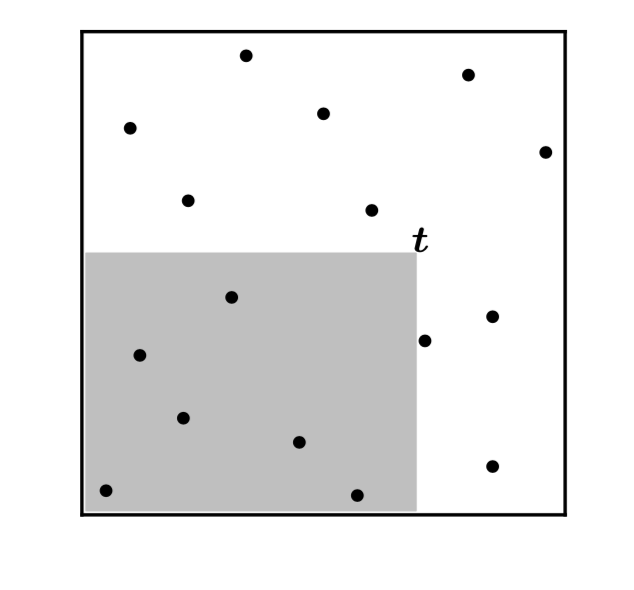
\includegraphics[width= 0.35\textwidth]{img/discrepancy/local_disc.png}
\caption{\label{fig:local_discrepancy}}
\end{figure}

 A discrepancy function of a design $\bm{x} \subset \X^{N}$ quantifies the "spread" of the nodes of $\bm{x}$. It is defined with respect to a set of test sets $\mathcal{S}$.





  For example, in $\mathcal{X} = [0,1]^{d}$, a typical choice of $\mathcal{S}$ is the set of the Cartesian products $[\bm{0},\bm{u}] = \prod\limits_{\delta \in [d]}[0,u_{\delta}]$ with $\bm{u} \in \mathcal{X}$. In this case, the local discrepancy is defined for all $\bm{u} \in \X$ by 
\begin{equation}\label{def:discrepancy}
\mathcal{D}_{\bm{x}}(\bm{u}) = \frac{1}{N}\sum\limits_{n \in [N]} \mathbb{1}_{[\bm{0},\bm{u}]}(x_{n}) - \prod\limits_{\delta \in [d]}u_{\delta}.
\end{equation}  
The term $\displaystyle \frac{1}{N}\sum\limits_{n \in [N]} \mathbb{1}_{[\bm{0},\bm{u}]}(x_{n})$ in \eqref{def:discrepancy} counts the number of the nodes $x_{n}$ that falls into $[\bm{0},\bm{u}]$ divided by the total number $N$; while the second term $\displaystyle  \prod\limits_{\delta \in [d]}u_{\delta}$ measures the volume of $[\bm{0},\bm{u}]$: $\mathcal{D}_{\bm{x}}$ measures the difference between the relative number of points that belongs to the interval $[0,\bm{u}]$ and its volume. A design of nodes $\bm{x}$ would be "well-spread" if the discrepancy function $\mathcal{D}_{\bm{x}}$ takes small values on $\X$. Therefore, a way to quantify the "spreadness" of $\bm{x}$ is to take an $\|.\|_{p}$ norm of $\mathcal{D}_{\bm{x}}$. Indeed, for $p \in [1,\infty]$, $\mathcal{D}_{\bm{x}} \in \mathbb{L}_{p}(\mathbb{R}^{d})$ because $\X = [0,1]^{d}$ is a compact set of $\mathbb{R}^{d}$; and the $\mathbb{L}_{p}$-discrepancy of $\bm{x}$ is defined by 
\begin{equation}
\Delta_{p}(\bm{x}) = \bigg(\int_{[0,1]^{d}}\mathcal{D}_{\bm{x}}(\bm{u})^{p} \mathrm{d}\bm{u}\bigg)^{1/p}.
\end{equation}
In particular, the $\|.\|_{\infty}$ norm of the local discrepancy is called the \emph{star-discrepancy} and it is denoted $\Delta_{*}(\bm{x})$.

Figure~\ref{fig:local_discrepancy} illustrates the concept of local discrepancy on $[0,1]^{2}$: the two hypercubes $[\bm{0},\bm{u}_{1}]$ and $[\bm{0},\bm{u}_{2}]$ have the same volume, yet the corresponding local discrepancies with respect to the design $\bm{x}$ are not equal as $[\bm{0},\bm{u}_{1}]$ contains more nodes from the design than $[\bm{0},\bm{u}_{2}]$.

Another example is the hypersphere $\X = \mathbb{S}^{d-1}$, where commonly considered test sets are the spherical caps defined by
\begin{equation}
C(t,\bm{u}) = \{ \bm{v} \in \mathbb{S}^{d-1}, \: \langle \bm{v}, \bm{u} \rangle \geq t\},
\end{equation}
and the local spherical discrepancy is defined by
\begin{equation}
...
\end{equation}
% where $t \in [-1,1]$ and $\bm{u} \in \mathbb{S}^{d-1}$ 
\paragraph{Koksma-Hlawka inequalities}
The importance of the discrepancy functions on bounding the integration error clears up considering the Koksma-Hlawka inequalities.
% The discrepancy functions for a design $\bm{x}$ play an important role in the quantification of the integration error based on $\bm{x}$. Indeed, consider the quadrature:
% \begin{equation}
% \frac{1}{N} \sum\limits_{n \in [N]}  f(x_{n}),
% \end{equation}
% as an approximation of $\displaystyle \int_{[0,1]^{d}} f(\bm{u}) \mathrm{d}\bm{u}$. 

\begin{theorem}\label{thm:KH_ineq}
Let $p,q \in [1,+\infty]$, such that $1/p+1/q = 1$. Consider $f \in \mathbb{L}_{q}([0,1]^{d})$. Then 
\begin{equation}\label{eq:KH_ineq}
\bigg| \int_{[0,1]^{d}} f(\bm{u}) \mathrm{d}\bm{u} - \frac{1}{N} \sum\limits_{n \in [N]}  f(x_{n})\bigg| \leq \Delta_{p}(\bm{x}) \|\frac{\partial^{d} f}{\partial \bm{u}}\|_{q}.
\end{equation}
\end{theorem}
The Koksma-Hlawka inequalities gives a decoupled upper bound for the integration error: the $\mathbb{L}_{p}$-discrepancy of the design $\bm{x}$ does not depend on $f$ and the $q$ variation of the function $f$ does not depend on the design $\bm{x}$. This decoupling allows to focus only on the discrepancy of the design when the function $f$ is sufficiently regular.

Koksma proved these inequalities for $d=1$, latter Hlawka generalised it to arbitrary dimension $d \geq 1$. Note that, initially, these inequalities were proven with the total variation in the sense of Hardy-Krause. Under some conditions ????, the total variation in the sense of Hardy-Krause coincide with $\|\frac{\partial^{d} f}{\partial \bm{u}}\|_{q}$ ??? 

In \citep{War72}, the author derived a tractable formula for the $\mathbb{L}_{2}$-discrepancy:

\begin{equation}
\Delta_{2}(\bm{x})^{2} = \frac{1}{3^{d}} - \frac{2}{N} \sum\limits_{n = 1}^{N} \prod\limits_{\delta=1}^{d} \frac{1-x_{n,i}^{2}}{2} + \frac{1}{N^2} \sum\limits_{n=1,n'=1}^{N} \prod\limits_{\delta=1}^{d} \min(1-x_{n,\delta},1-x_{n',\delta}).
\end{equation}

We shall give an interpretation of this formula in the context of kernel quadrature. For the moment, it is enough to observe that the minimal value of $\displaystyle  \Delta_{2}(\bm{x})^{2}$ is $\displaystyle \frac{1}{3^{d}}$ achieved when the design $\bm{x}$ is empty.

This situation is to be compared to the star discrepancy for witch no tractable formula is known: the computation of the star discrepancy is an NP-hard problem \citep{GnSrWi09}.

From a distance, a regular lattice is "well-spread" in the hypercube $[0,1]^{d}$ and would be a good choice for the design $\bm{x}$. Unfortunately, this is a false-intuition regarding the following proposition. 

\begin{proposition}
Let $n = \nu^{d}$ where $\nu \in \mathbb{N}^{*}$, and define the regular lattice $\bm{x} \in \mathbb{R^{d}}^{n}$ by 
\begin{equation}
\bm{x} = \{ (\frac{\nu_{1}}{\nu}, \dots, \frac{\nu_{d}}{\nu}), \: 0 \leq \nu_{\delta} < \nu, \delta \in [d] \}. 
\end{equation}
Then
\begin{equation}
\Delta_{*}(\bm{x}) = 1- (1-1/\nu)^{d} \geq \frac{1}{n^{1/d}}. 
\end{equation} 
\end{proposition}

In other words, in order to get a star-discrepancy lower than some level $\epsilon \in [0,1[$, we need $n = \Omega(\epsilon^{1/d})$ nodes: the star discrepancy of the regular lattice scales poorly with the dimension; even tough it have the best possible star discrepancy when $d = 1$. 


Looking for designs having the lowest discrepancy in high dimension was a topic of intense research.  A very brief review of this line of research is provided in the following paragraph. 
\paragraph{Low discrepancy sequences}
The van der Corput sequence is the simplest example of a low discrepancy sequence in $[0,1]$ and allows the construction of low discrepancy sequences in $[0,1]^{d}$.
\begin{definition}
Let $b \geq 2$ be an integer. Let $n \in \mathbb{N}$, and consider its $b$-adic expansion:
\begin{equation}
n = \sum\limits_{i \in \mathbb{N}} n_{i}b^{i}.
\end{equation} 
The $b$-adic van der Corput sequence is the sequence $(v_{b,n})_{n \in \mathbb{N}}$, where for every $n \in \mathbb{N}$, 
\begin{equation}
v_{b,n} = \sum\limits_{i \in \mathbb{N}} n_{i}b^{-i}. 
\end{equation}
\end{definition}
For instance, for $b = 2$, the first elements of the corresponding van der Corput sequence are $\displaystyle 0, \frac{1}{2}, \frac{3}{4}, \frac{1}{8}, \frac{5}{8}, \frac{3}{8}, \dots$

\begin{definition}
Let $b_{1}, \dots, b_{d}$ be a sequence of integers larger than $2$. The Halton sequence is defined by
\begin{equation}
x_{n} = (v_{b_1,n}, \dots, v_{b_d,n})
\end{equation}
\end{definition}
We have the following upper bound on the star-discrepancy of the Halton sequence.
\begin{theorem}
Assume that the $b_{1}, \dots, b_{d}$ are pairwise relatively prime, and let $\bm{x}$ the corresponding Halton sequence. Then
\begin{equation}
\Delta_{*}(\bm{x}) \leq c(b_{1}, \dots, b_{d}) \frac{(\log n)^{d}}{n} + \mathcal{O}\bigg(\frac{(\log n)^{d-1}}{n} \bigg),
\end{equation}
where 
\begin{equation}
c(b_{1}, \dots, c_{d}) = \frac{1}{d!} \prod\limits_{\delta \in [d]} \frac{\lfloor b_{\delta}/2 \rfloor }{\log b_{i}}.
\end{equation}
Morover, if $b_{1}, \dots, b_{d}$ are the fist $d$ prime numbers, then 
\begin{equation}
c(b_{1}, \dots, b_{d}) \leq \frac{7}{2^{d}d}.
\end{equation}
\end{theorem}

The star discrepancy of the Halton sequence is $\displaystyle \mathcal{O}(\frac{(\log N)^{d}}{N})$. Based on the Halton sequence, one can build the Hammersley point sets as follows. 
\begin{definition}
Assume that $d \geq 2$, and let $b_{1}, \dots, b_{d-1}$ integers larger than $2$.
The Hammersley point set $\{x_{1}, \dots, x_{N} \}$ consisting of $N$ nodes and associated to the bases $b_{1}, \dots, b_{d-1}$ is defined by
\begin{equation}
x_{n} = ((n-1)/N,v_{b_1,n}, \dots, v_{b_{d-1},n}).
\end{equation}
\end{definition}




The star discrepancy of the Hammersley point sets scales as $\displaystyle \mathcal{O}(\frac{(\log N)^{d-1}}{N})$ which is a better rate than the Halton sequence rate.


Lattice point sets is another family of designs that contains some low discrepancy sequences.

\begin{definition}
Let $\bm{g} \in \mathbb{N}^{d}$, $N \in \mathbb{N}$. A lattice point set of generating vector $\bm{g}$ is the design $\bm{x}$ defined by
\begin{equation}
x_{n} = \{ n\bm{g}/N \}.
\end{equation}
\end{definition}

The star discrepancy of a lattice is tractable and it is given by ...

\begin{proposition}
\begin{equation}
\Delta_{*}(\bm{x}) \leq \frac{d}{N} + \frac{1}{2} \sum\limits_{h ...}
\end{equation}
\end{proposition}

This family of sequence is 


....


....

....


\begin{figure}
\centering
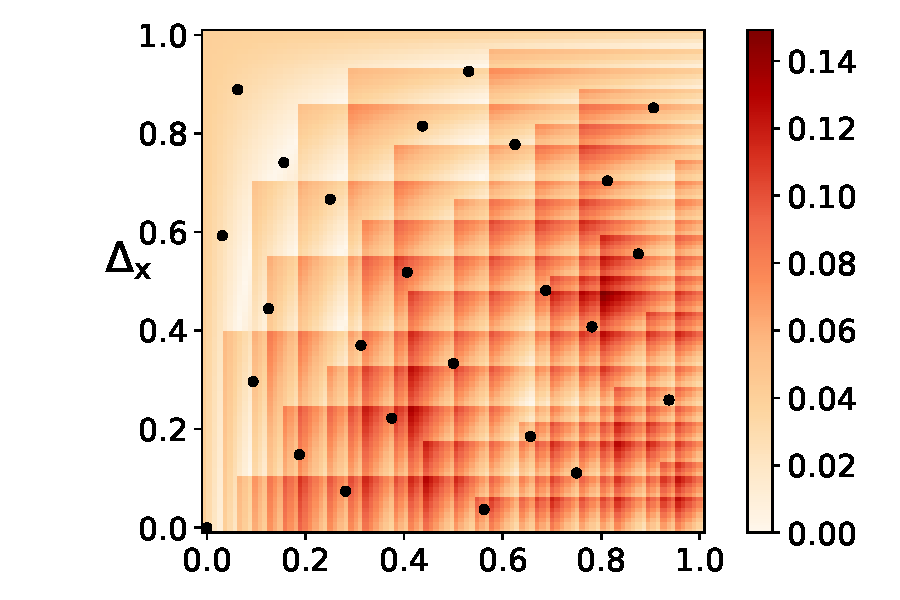
\includegraphics[width= 0.32\textwidth]{img/discrepancy/local_discrepancy_halton_N_25.pdf}~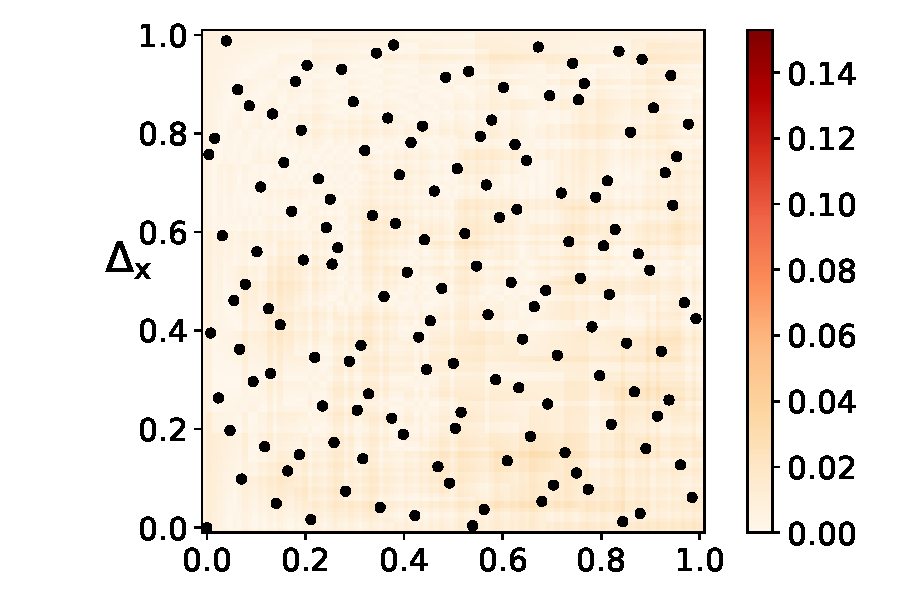
\includegraphics[width= 0.32\textwidth]{img/discrepancy/local_discrepancy_halton_N_144.pdf}
~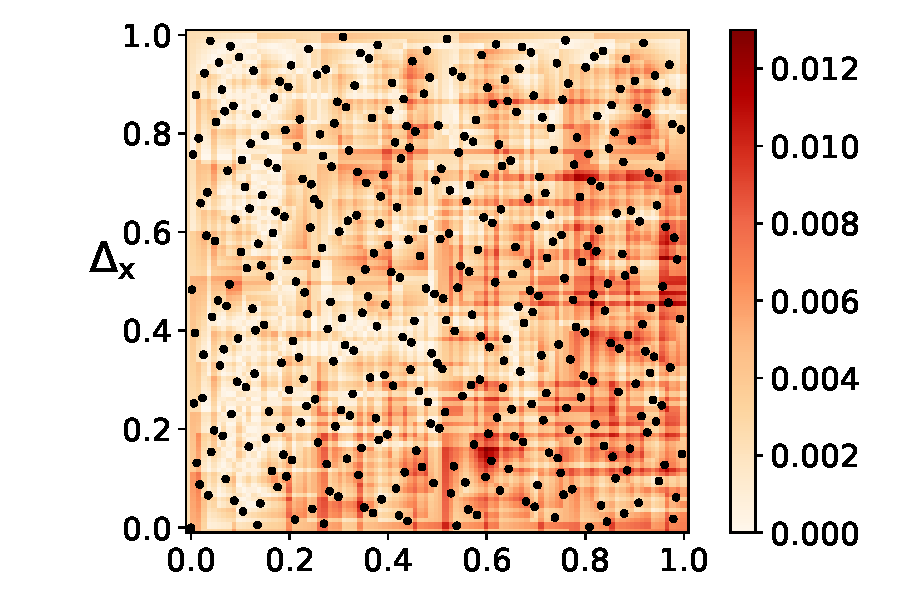
\includegraphics[width= 0.32\textwidth]{img/discrepancy/local_discrepancy_halton_N_400.pdf}\\
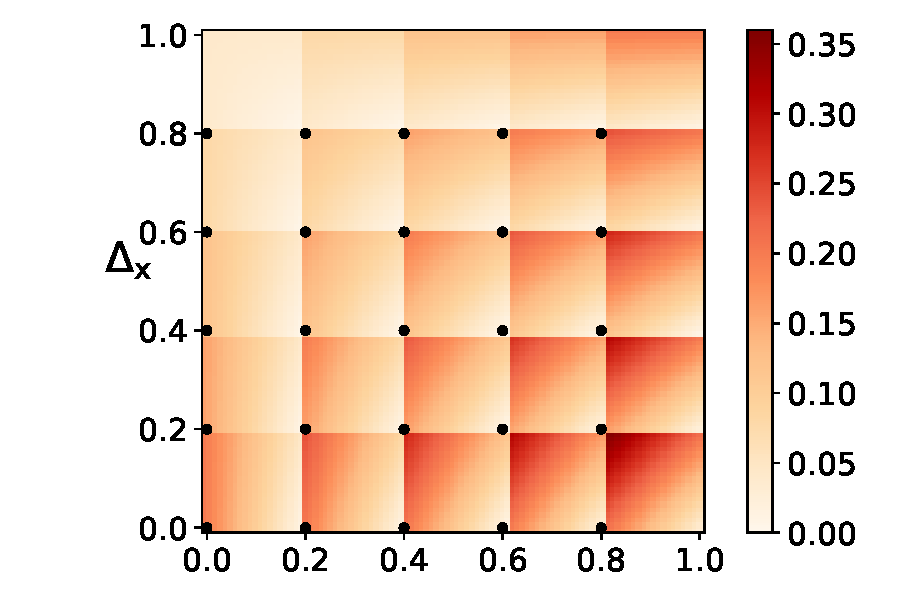
\includegraphics[width= 0.32\textwidth]{img/discrepancy/local_discrepancy_uniform_grid_N_25.pdf}~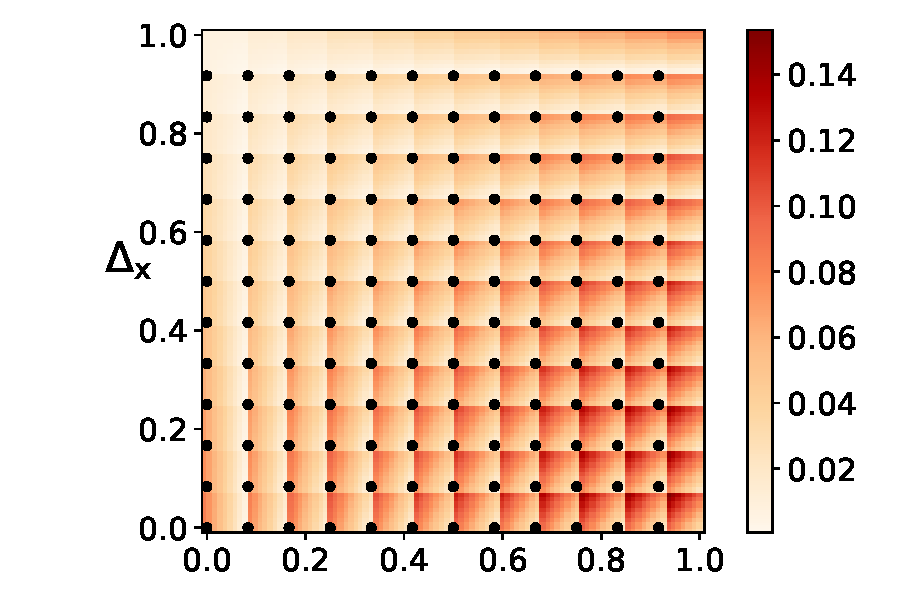
\includegraphics[width= 0.32\textwidth]{img/discrepancy/local_discrepancy_uniform_grid_N_144.pdf}
~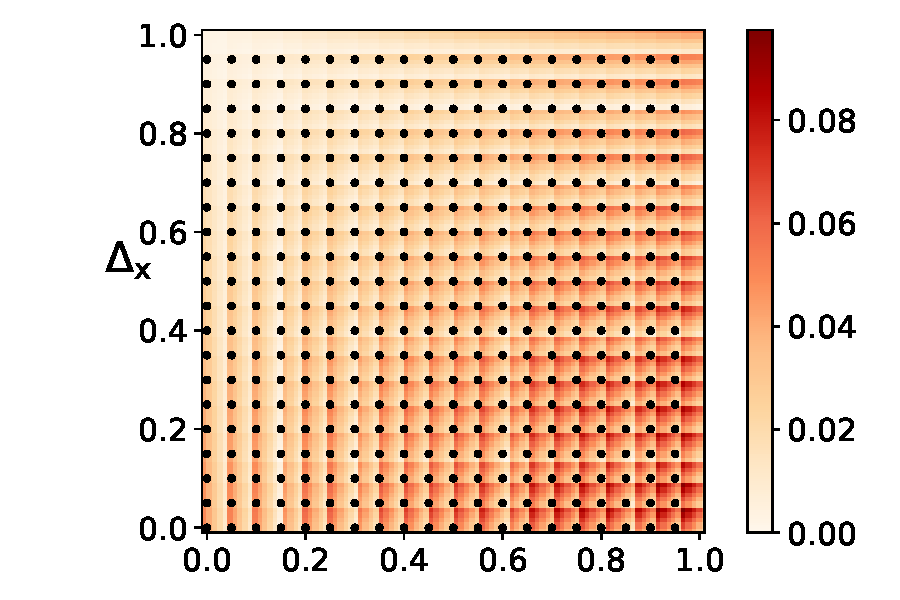
\includegraphics[width= 0.32\textwidth]{img/discrepancy/local_discrepancy_uniform_grid_N_400.pdf}
\caption{The local discrepancy $\Delta_{\bm{x}}$ for two designs: in the top, the Halton sequence with $N \in \{25,144,400\}$; in the bottom, the uniform grid with $N \in \{25,144,400\}$.}
\end{figure}

\subsubsection{DPPs for numerical integration}
Determinantal point processes were used as design nodes of quadratures with fast rates of convergence. We review in this section, the results and the techniques used in this line of research. 

\paragraph{Johansson CLT and the Szegő limit theorems}
We start by the Centrale Limite Theorem result of Johansson of the linear statistic under a specific projection DPP.

\begin{theorem}
Let $f: \mathbb{U}_{N} \rightarrow \mathbb{C}$ that satisfies
\begin{equation}\label{eq:weil_condition}
\forall \: V, M \in \mathbb{U}_{N}, \:  f(V^{-1}M V) = f(M),
\end{equation}
and denote for $\bm{\theta} = (\theta_{n})_{n \in [N]} \in [0,2\pi]^{N}$, the diagonal matrix $D(\bm{\theta}) = \mathrm{diag}(e^{i \theta_{n}})_{n \in [N]}$.
Then
\begin{equation}
\int_{\mathbb{U}_{N}}f(M) \mathrm{d}M = \frac{1}{N!(2 \pi)^{N}} \int_{[0,2\pi]^{N}} f(D(\theta)) \Delta(\theta)^{2} \mathrm{d}^{N}\theta,
\end{equation}
where 
\begin{equation}
\Delta(\theta) = \prod\limits_{1 \leq n,n' \leq N} | e^{i \theta_{n}} -e^{i \theta_{n'}} |.
\end{equation}
\end{theorem}

In other words, the joint distribution of the eigenvalues of a random unitary matrix with respect to Haar measure have the probability density:
\begin{equation}\label{eq:haar_eigenvalues_density}
\frac{1}{N!(2\pi)^{N}} \prod\limits_{1 \leq n,n' \leq N} |e^{-i \theta_{n}} - e^{-i \theta_{n'}}|^{2}
\end{equation}
on $\mathbb{U}^{N}$.
The trace function $f = \Tr$ satisfies the condition~\eqref{eq:weil_condition}; thus as a corollary we have the following identity:
\begin{equation}
\int_{\mathbb{U}_{N}}\Tr(M) \mathrm{d}M = \frac{1}{N!(2 \pi)^{N}} \int_{[0,2\pi]^{N}} \Tr(D(\theta)) \Delta(\theta)^{2} \mathrm{d}^{N}\theta.
\end{equation}

Let $g \in \mathbb{L}_{1}(\mathbb{T})$, and $N \in \mathbb{N}^{*}$. Denote by $\bm{T}_{N}(g)$ the Toeplitz determinant with respect to the symbol $g$:
\begin{equation}
\bm{T}_{N}(g) = \Det(\hat{g}_{n-n'})_{0 \leq n,n' \leq N-1}.
\end{equation}
\begin{theorem}
Let $g \in \mathbb{L}_{1}(\mathbb{T})$ be a complex-valued function on $\mathbb{T}$ with Fourier coefficients $(\hat{g}_{n})_{n \in \mathbb{Z}}$. Assume that $\displaystyle \sum\limits_{n \in \mathbb{Z}} |n||\hat{g}_{n}|^{2} < +\infty$. Then
\begin{equation}
\bm{T}_{N}(g) = e^{N\hat{g}_{0} + \sum\limits_{n  =1}^{+\infty}n \hat{g}_{-n} \hat{g}_{n} + o(1)},
\end{equation}
as $N \rightarrow +\infty$.
\end{theorem}

This allowed the author to prove the following CLT.
\begin{theorem}
Let $g \in \mathbb{L}_{1}(\mathbb{T})$ such that $\displaystyle \sum\limits_{n \in \mathbb{N}^{*}} n|\hat{g}_{n}|^{2} <+\infty$. Let $\bm{\theta} = (\theta_{n})_{n \in [N]} \in [0,2\pi]^{N}$ a random vector, such that the joint distribution of $(\theta_{1}, \dots, \theta_{N})$ have the density~\eqref{eq:haar_eigenvalues_density}. Then the random variable
\begin{equation}
\frac{1}{N}\sum\limits_{n \in [N]} g(\theta_{n}), 
\end{equation}
converges to $\displaystyle \mathcal{N}(0,\frac{2}{N}\sum\limits_{n \in \mathbb{N}^{*}} n|\hat{g}_{n}|^{2})$.
\end{theorem}



\begin{figure}
\centering
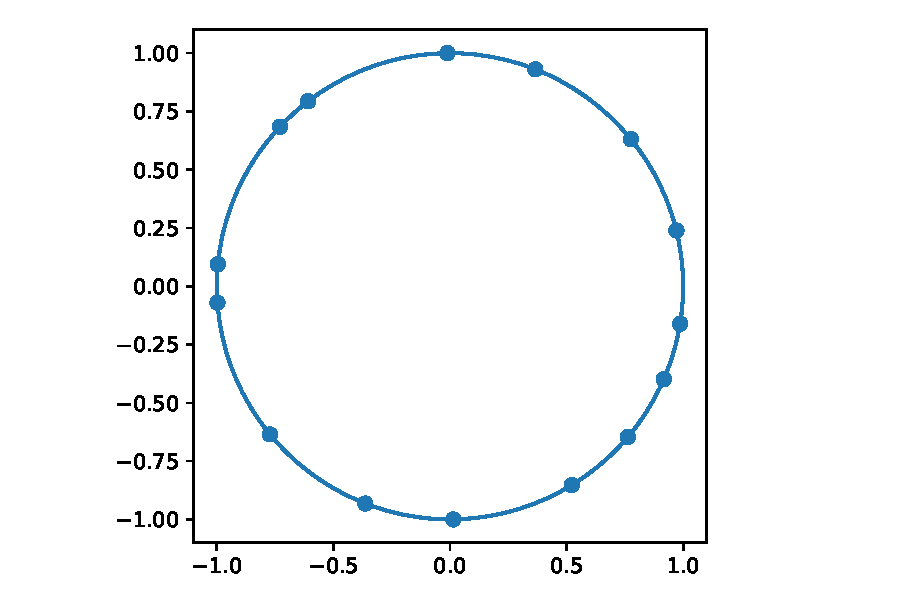
\includegraphics[width= 0.32\textwidth]{img/circle/CUE_design_N_15_fig_1.pdf}~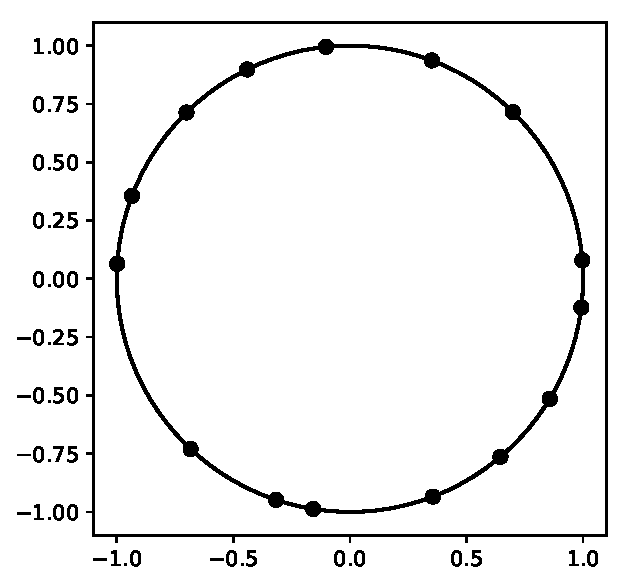
\includegraphics[width= 0.32\textwidth]{img/circle/CUE_design_N_15_fig_2.pdf}
~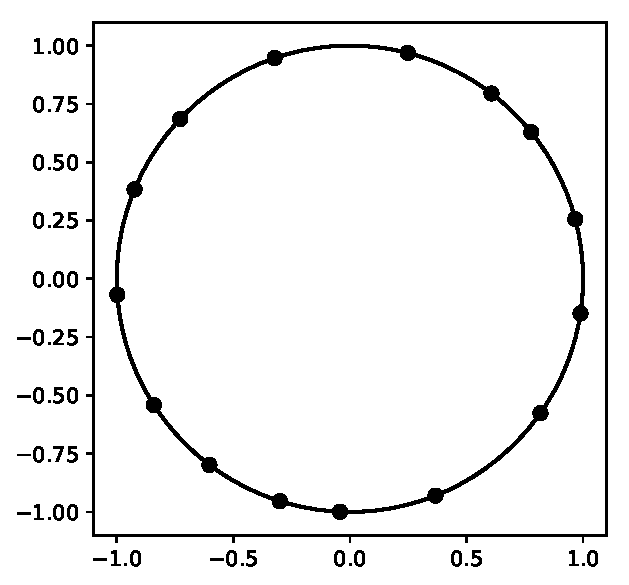
\includegraphics[width= 0.32\textwidth]{img/circle/CUE_design_N_15_fig_3.pdf}\\
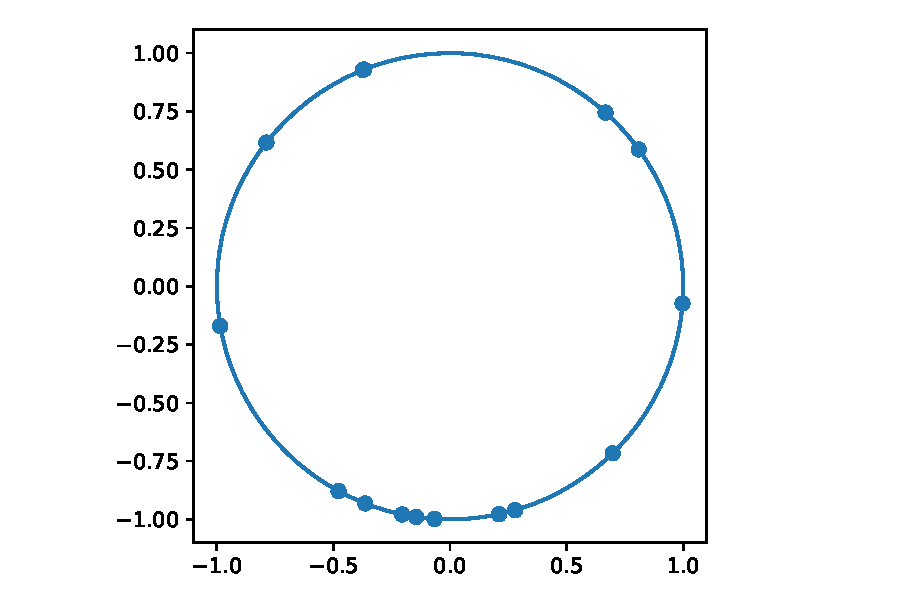
\includegraphics[width= 0.32\textwidth]{img/circle/iid_design_N_15_fig_1.pdf}~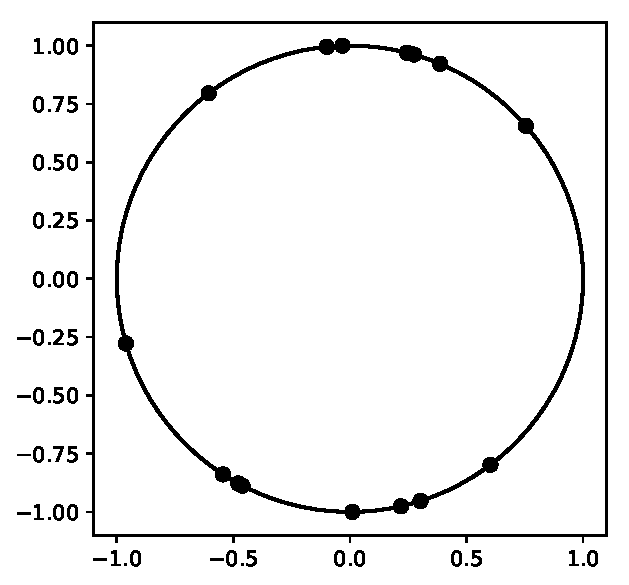
\includegraphics[width= 0.32\textwidth]{img/circle/iid_design_N_15_fig_2.pdf}
~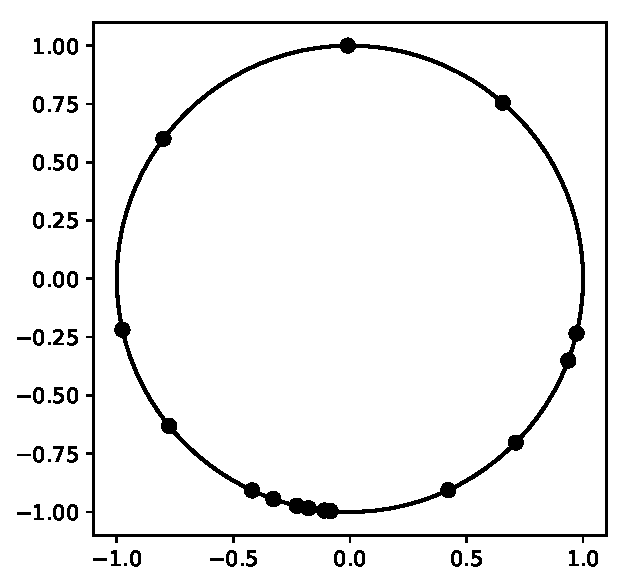
\includegraphics[width= 0.32\textwidth]{img/circle/iid_design_N_15_fig_3.pdf}\\
\caption{Three realizations from the CUE of 15 particles (top) compared to 15 particles sampled i.i.d in the unit circle (bottom).}
\end{figure}

\paragraph{CLT using Orthogonal Polynomial Ensembles}

In \citep{BaHa16}, the authors proved the first CLT for a quadrature based on nodes that follow the distribution of a determinantal point process for functions defined on high dimension domains. In particular, this work dealed with quadratures defined on the integration domain $[-1,1]^{d}$ for the approximation of integrals that write
\begin{equation}
\int_{[-1,1]^{d}} f(x) \mathrm{d}\omega(x),
\end{equation}
for a measure $\mathrm{d}\omega$ that  factorized as
\begin{equation}
\mathrm{d}\omega(x) = \prod\limits_{\delta \in [d]} \mathrm{d}\omega_{\delta}(x_{\delta}),
\end{equation}
where the measures $\mathrm{d}\omega_{\delta}$, defined on $[-1,1]$, belong to what is called \emph{Nevai class}. We recall the definition of this class of measures in the following.

\begin{definition}


Let $\mathrm{d}\tilde{\omega}$ a measure on the real line supported on $[-1,1]$. Denote by $(a_{m})_{m \in \mathbb{N}}$ and $(b_{m})_{m \in \mathbb{N}}$ the sequences of coefficients appearing in the three-term recurrence relation:
\begin{equation}
t P_{m}(t) = a_{m}P_{m+1}(t) + b_{m}P_{m}(t) + a_{m-1}P_{m-1}(t),
\end{equation}
associated to the sequence of orthogonal polynomials $(P_{m})_{m \in \mathbb{N}}$ with respect to $\mathrm{d}\tilde{\omega}$.

The measure $\mathrm{d}\tilde{\omega}$ is said to be of Nevai class if and only if
\begin{equation}
\lim\limits_{m \rightarrow +\infty} a_{m} = 1/2, \:\:\: \lim\limits_{m \rightarrow +\infty} b_{m} = 0.
\end{equation}
\end{definition}
The particular case when 
\begin{equation}
\forall m \in \mathbb{N}, \:\: a_{m} = \frac{1}{2}, \:\: b_{m} =0,
\end{equation}
corresponds to the Chebyshev orthogonal polynomials of the first kind; and the corresponding measure $\mathrm{d}\tilde{\omega}^{*}$ admits a density $\tilde{\omega}^{*}$ with respect to the Lebesgue measure:
\begin{equation}
\tilde{\omega}^{*}(x) = \frac{1}{\sqrt{1-x^{2}}}.
\end{equation}

In other words, the Nevai class contains measures that have three terms coefficients converging to the corresponding coefficients of $\mathrm{d}\tilde{\omega}^{*}$.

A sufficient condition for a measure to be Nevai class is given in the following result.
\begin{theorem}
Let $\mathrm{d}\omega$ be a measure supported on $[-1,1]$, and consider its Lebesgue decomposition:
\begin{equation}
\mathrm{d}\omega = \omega(x) \mathrm{d}x + \mathrm{d}\omega_{s}.
\end{equation}
If $\omega(x) >0$ almost everywhere, then $\mathrm{d}\omega$ is Nevai-class.
\end{theorem}

Now for a given measure $\mathrm{d}\omega$ that decomposes as the product of $d$ Nevai class measures $\mathrm{d}\omega_{\delta}$, define ....

and the projection kernel
\begin{equation}
\KDPP(x,y) = \sum\limits_{n \in [N]} ...
\end{equation} 

\begin{theorem}
Let $\mu$ be a reference measure such that it's support is included in $[0,1]^{d}$, and assume that $\mu = \mu_{1} \otimes \dots \otimes \mu_{d}$, where each $\mu_{\delta}$ is Nevai class. 


Then for every $f \in \mathcal{C}^{1}([0,1]^{d}, \mathbb{R})$,

\begin{equation}
\frac{1}{\sqrt{N^{1-1/d}}} \big( \sum\limits_{n \in [N]}f(x_{n}) - ... \big) \rightarrow \mathcal{N}(0,\sigma^{2}(f)),
\end{equation}
where
\begin{equation}
\sigma^{2}(f) = \frac{1}{2} \sum\limits_{m_{1}, \dots , m_{d} = 0}^{+\infty} (m_{1}+\dots +m_{d}) \hat{f}(m_{1}, \dots, m_{d})^{2},
\end{equation}
and 
\begin{equation}
\hat{f}(m_{1},\dots,m_{d}) = \int_{[-1,1]^{d}} f(u_{1}, \dots, u_{d}) \prod\limits_{\delta \in [d]} T_{m_{\delta}}(u_{\delta}) \frac{1}{\pi \sqrt{1-u_{\delta}^{2}}} \mathrm{d}u_{\delta}
\end{equation}

\end{theorem}

\paragraph{CLT using the Dirichlet kernel}
In \citep*{CoMaAm20}, the authors proposed to study a quadrature based on a different projection DPP and using uniform weights. The integrand $f$ was assumed to be square integrable and periodic on the hypercube $[0,1]^{d}$. The repulsion kernel $\KDPP$ is constructed as following. The authors assumed that there exists $N_{1}, \dots, N_{d} \in \mathbb{N}^{*}$ such that $N = \prod\limits_{\delta \in [d]}N_{\delta}$; and the projection DPP is defined by
\begin{equation}\label{eq:Dirichlet_kernel}
\KDPP(x,x) = \sum\limits_{\bm{m} \in \mathcal{M}_{N}}e^{2i \pi \bm{m}^{\Tran}(x-y) },
\end{equation}
where 
\begin{equation}
\mathcal{M}_{N} = \prod\limits_{\delta \in [d]} \{0, \dots, N_{\delta}-1 \}.
\end{equation}
The definition of the set $\mathcal{M}_{N}$ is not canonical and can be replaced by
\begin{equation}
\mathcal{M}_{N} = \prod\limits_{\delta \in [d]} \{-\lfloor{N_{\delta}/2}\rfloor, \dots, \lfloor{N_{\delta}/2}\rfloor \},
\end{equation}
if the $N_{\delta}$ are odds, which lead to the tensor product of Dirichlet kernels. For this reason, the authors adopted the name of $(N,d)$-Dirichlet DPP for the projection DPP associated to the kernel~\eqref{eq:Dirichlet_kernel}.

This quadrature defines an unbiased estimator of the integral $\int_{[0,1]^{d}} f(\bm{u}) \mathrm{d}\bm{u}$ with a variance that depends on the Fourier coefficients of $f$. 
\begin{proposition}\label{prop:dirichlet_estimator} [Proposition 3.1, \citep{CoMaAm20} ]
Let $\bm{x}$ a random set of $[0,1]^{d}$ that follows the distribution of $(N,d)$-Dirichlet DPP, and $f \in \mathbb{L}_{2}([0,1]^{d})$ and periodic; and define, 
\begin{equation}
\hat{I}_{N}(f) =  \frac{1}{N} \sum\limits_{n \in [N]}f(x_{n}).
\end{equation}
Then, $\hat{I}_{N}(f)$ is an unbiased estimator of $\displaystyle \int_{[0,1]^{d}} f(\bm{u})\mathrm{d}\bm{u}$, and
\begin{equation}
\Var (\hat{I}_{N}(f)) = \frac{1}{N}\sum\limits_{\bm{m} \in \mathbb{Z}^{d}} |\hat{f}_{\bm{m}}|^{2} - \frac{1}{N^2} \sum\limits_{\bm{m}_{1},\bm{m}_{2} \in \mathcal{M}_{N}} |\hat{f}_{\bm{m}_{1}-\bm{m}_{2}}|^{2},
\end{equation}
where
\begin{equation}
 \hat{f}_{\bm{m}} = \int_{[0,1]^{d}}f(\bm{u}) e^{- 2\pi i \bm{m}^{\Tran}\bm{u}} \mathrm{d}\bm{u}.
\end{equation}

% where
% \begin{equation}
% \mathcal{M}_{N} = \{\bm{m} \in \mathbb{Z}^{d}, \: m_{\delta} \leq N_{\delta} -1, \delta \in [d]\}.
% \end{equation}

\end{proposition}


This result was the first step for the asymptotic analysis of the variance of $\hat{I}_{N}(f)$ under the assumption that $N_{\delta} = N_{\delta}(N)$, and there exists constants $\alpha_{1}, \dots, \alpha_{d}$ such that
\begin{equation}
\forall \delta \in [d], \:\:\lim\limits_{N \rightarrow +\infty} N_{\delta}(N)N^{-1/d} = \alpha_{\delta}.
\end{equation}

Define $\mathcal{F}_{s}([0,1]^{d})$ to be the subspace of periodic elements of $\mathbb{L}_{2}([0,1]^{d})$ that satisfy the condition
\begin{equation}
\sum\limits_{\bm{m} \in \mathbb{Z}^{d}} (1+ \|\bm{m}\|_{\infty})^{2s} |\hat{f}(\bm{m})|^{2} < +\infty.
\end{equation}




\begin{theorem}
Let $\bm{x}$ and $f$ as in Proposition~\ref{prop:dirichlet_estimator}. Assume that $f \in \mathcal{F}_{s}([0,1]^{d})$, then
\begin{itemize}
\item if $s \in [0,1/2]$, then 
\begin{equation}
\Var (\hat{I}_{N}(f))  = \mathcal{O}(N^{-1-\frac{2s}{d}}),
\end{equation}
\item If $s>1/2$, then
\begin{equation}
\lim\limits_{N \rightarrow +\infty} N^{1+1/d} \Var (\hat{I}_{N}(f)) = \sigma^{2}(f) := \sum\limits_{\bm{m} \in \mathbb{Z}^{d}}(\sum\limits_{\delta = 1}^{d} \frac{|m_{\delta}|}{\alpha_{\delta}} ) |\hat{f}_{\bm{m}}|^{2}.
\end{equation}
\item Moreover, if $s>1/2$ and $ \|f\|_{\infty} < +\infty$, then
\begin{equation}
\sqrt{N^{1+1/d}} \left(\hat{I}_{N}(f) - \int_{[0,1]^{d}}f(\bm{u})\mathrm{d}\bm{u} \right) \rightarrow \mathcal{N}(0,\sigma^{2}(f)).
\end{equation}
\end{itemize}

\end{theorem}
\subsection{The kernel framework for quadratures}


The analysis of quadratures using kernel methods is convenient and elegant at the same time and it is expressed using functional analysis tools similarly to DPPs. Added to that, many results in quasi-Monte Carlo theory have an interpretation within the kernel quadrature framework. 

The strength of this framework is its flexibility: the integration domain $\mathcal{X}$ is assumed to be a metric space endowed with a Borel measure $\mathrm{d}\omega$, and we consider approximating an integral $\displaystyle \int_{\X} f(x)g(x)\mathrm{d}\omega(x)$, where $f,g \in \mathbb{L}_{2}(\mathrm{d}\omega)$ and $f$  is continuous, using a quadrature rule $(\bm{x}, \bm{w}) \in \X^{N} \times \mathbb{R}^{N}$:
\begin{equation}\label{eq:int_error}
\int_{\X} f(x)g(x)\mathrm{d}\omega(x) \approx \sum\limits_{n \in [N]} w_{n} f(x_{n}),
\end{equation}

where $\mathbb{L}_{2}(\mathrm{d}\omega)$ is the Hilbert space of square integrable, real-valued functions defined on $\mathcal{X}$, with the usual inner product denoted by $\langle \cdot, \cdot \rangle_{\mathrm{d}\omega}$, and the associated norm by $\|.\|_{\mathrm{d}\omega}$.

As we shall see, the analysis of the integration error in~\eqref{eq:int_error} is convenient if $f$ belongs to a Reproducing Kernel Hilbert Space (RKHS).

In the following sections, we recall the essential notions on kernel methods needed for the analysis of the integration error of a function that belongs to an RKHS, along with a review of the existing nodes design paradigms. In Section~\ref{subsec:rkhs}, we recall the definition of RKHSs and the interpretations of the required conditions we assume; in Section~\ref{subsec:mercer}, we recall the Mercer theorem- required to outline the main results of this chapter- and its various extensions to non-compact domains; in Section~\ref{subsec:int_error}, we recall a classic upper bound of the integration error via the definition of the worst integration error on an RKHS; in Section~\ref{subsec:kernel_examples}, we give some examples of kernels widely used in the literature of kernel quadrature; in Section~\ref{subsec:bayesian_quadrature}, we recall the link between kernel quadrature and Gaussian processes approximations along with Bayesian quadrature; in Section~\ref{subsec:okq_analysis_paradigm} and Section~\ref{subsec:okq_algebraic_paradigm}, we review the two paradigms of nodes design for kernel quadratures.
\subsubsection{Reproducing Kernel Hilbert Spaces}\label{subsec:rkhs}

We start by the definition of a kernel over $\mathcal{X}$. A function $k: \mathcal{X} \times \mathcal{X} \rightarrow \mathbb{R}_{+}$ is said to be a kernel over $\mathcal{X}$ if $k$ is symmetric and for any finite set of points in $\mathcal{X}$, the matrix of pairwise kernel evaluations is positive semi-definite.

An RKHS over $\mathcal{X}$ is a Hilbert space $\mathcal{F}$ endowed with a kernel $k$ that satisfies the following two properties:
\begin{itemize}
\item the continuity property: for every $x \in \mathcal{X}$, the evaluation function $f \mapsto f(x)$ is continuous with respect to the norm of $\mathcal{F}$ 

\begin{equation}
\forall x \in \mathcal{X}, \: \exists M_{x} >0 , \: \forall f \in \mathcal{F}, \: |f(x)| \leq M_{x} \|f\|_{\mathcal{F}},\nonumber
\end{equation} 
\item the reproducibility property:\begin{equation}
\forall (x,f) \in \mathcal{X}\times\mathcal{F}, \: f(x) = \langle f, k(x,.) \rangle_{\mathcal{F}}. \nonumber
\end{equation}
\end{itemize}
 
Usually the kernel $k$ is assumed to be continuous with respect to the induced topology of $\mathcal{X} \times \mathcal{X}$. We assume that this condition is satisfied in the following. We discuss later, a case where it is not verified.
The requirement that can be embedded in $\mathbb{L}_{2}(\mathrm{d}\omega)$


 To see this, let  Denote by $\mathcal{F}$ the associated reproducing kernel Hilbert space (RKHS) of real-valued functions \cite{BeTh11}. We assume that $x \mapsto k(x,x)$ is integrable with respect to the measure $\mathrm{d}\omega$ so that $\mathcal{F} \subset \mathbb{L}_{2}(\mathrm{d}\omega)$.



% In order to present this framework, we introduce some notations.

% First, we denote by $\mathcal{X}$ . $\mathcal{X}$ is assumed to be a metric space endowed with a Borel measure $\mathrm{d}\omega$.
% This analysis is based on the following observation: if $f : $
% Denote by $(e_{k})_{k \in \mathbb{N}}$ an orthonormal family of $\mathbb{L}_{2}(\mathrm{d}\omega)$.
%
 
%$$\mathcal{F} = \overline{\Span \bigg( k(x,.),\: x \in \mathcal{X} \bigg)}$$
\begin{figure}[]
    \centering
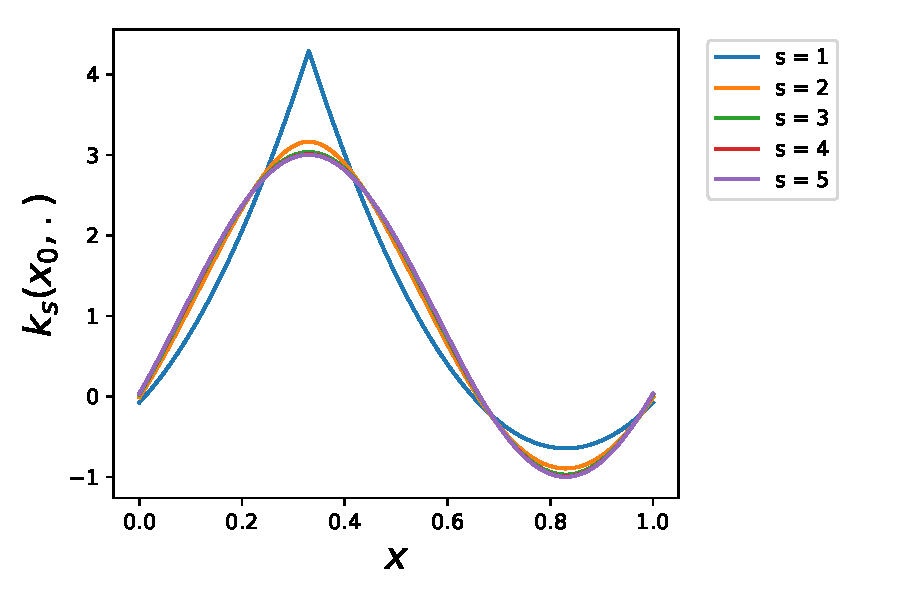
\includegraphics[width= 0.75\textwidth]{img/Sobolev/Bernoulli_kernels_same_node_s_1_5.pdf}
\caption{The evaluation of the kernel $k_{s}$ for $s \in \{1,2,3,4,5\}$.
\label{fig:periodic_sobolev_kernel}}
\end{figure}



\subsubsection{The Mercer decomposition}
\label{subsec:mercer}
The Mercer Theorem was first proven when $\mathcal{X} = [0,1]$ and $\mathrm{d}\omega$ is the Lebesgue measure in \cite{Mer1909}.
A modern proof of this classic result can be found in \cite{Lax02}. An extension to a general compact space $\mathcal{X}$ can be  found in \cite{CuZh07}. To state this classic result, we consider the integration operator
% In this section we recall Mercer's theorem and its extensions to non-compact spaces. Let $\mathcal{X}$ be a measurable space and $\mathrm{d}\omega$ a measure on $\mathcal{X}$. 

% Assume $k$ is a positive definite kernel on $\mathcal{X}$. Whenever it is well-defined, we consider the operator
\begin{equation}
\bm{\Sigma} f(x) = \int\limits_{\mathcal{X}} k(x,y)f(y) \mathrm{d}\omega(y).
\end{equation}
\begin{theorem}\label{thm:Mercer_for_compact}
Assume that $\mathcal{X}$ is a compact space and $\mathrm{d}\omega$ is a finite Borel measure on $\mathcal{X}$.
Then, there exists an orthonormal basis $(e_{n})_{n \in \mathbb{N}^{*}}$ of $\mathbb{L}_{2}(\mathrm{d}\omega)$ consisting of eigenfunctions of $\bm{\Sigma}$, and the corresponding eigenvalues are non-negative.
The eigenfunctions corresponding to non-vanishing eigenvalues can be taken to be continuous, and the kernel $k$ writes
\begin{equation}
k(x,y) = \sum\limits_{n \in \mathbb{N}^{*}} \sigma_{n} e_{n}(x)e_{n}(y),
\end{equation}
where the convergence is absolute and uniform.
\end{theorem}
   Note, however, that the compactness assumption in Theorem~\ref{thm:Mercer_for_compact} excludes kernels such as the Gaussian or the Laplace kernels.
Hence, extensions to non-compact spaces are usually required in ML.
In \cite{Sun05}, the author extended Theorem~\ref{thm:Mercer_for_compact} to $\mathcal{X} = \cup_{i \in \mathbb{N}} \mathcal{X}_{i}$, with the $\mathcal{X}_{i}$s compact and $\mathrm{d}\omega(\mathcal{X}_{i})<\infty$. One can also extend Mercer's theorem under a \textit{compact embedding} assumption \citep{StSc12}: the RKHS $\mathcal{F}$ associated to $k$ is said to be compactly embedded in $\mathbb{L}_{2}(\mathrm{d}\omega)$ if the application
\begin{align*}
  I_{\mathcal{F}}: \mathcal{F}&\longrightarrow \mathbb{L}_{2}(\mathrm{d}\omega) \\
  f &\longmapsto f
\end{align*}
is compact.
A sufficient condition for this assumption is the integrability of the diagonal (Lemma 2.3, \citep{StSc12}):
\begin{equation}
\int_{\mathcal{X}} k(x,x) \mathrm{d}\omega(x) < \infty.
\end{equation}
Note that this condition is not necessary (Example 2.9, \citep{StSc12}). Now, under the compact embedding assumption, the pointwise convergence of the Mercer decomposition to the kernel $k$ is equivalent to the injectivity of the embedding $I_{\mathcal{F}}$ (Theorem 3.1, \citep{StSc12}).
% This condition is satisfied whenever $k$ is bounded and $\mathrm{d}\omega(\mathcal{X}) < \infty$.
% \begin{theorem}[Theorem 3.1, \cite{StSc12}]
% Let $\mathcal{X}$ be a measurable space and $\mathrm{d}\omega$ a measure on $\mathcal{X}$. Let $k$ be a measurable positive kernel on $\mathcal{X}$ with an RKHS $\mathcal{F}$. Assume that $\mathcal{F}$ is compactly embedded in $\mathbb{L}_{2}(\mathrm{d}\omega)$. Define the integral operator $\bm{\Sigma}$:
% \begin{equation}
% \bm{\Sigma} f(x) = \int\limits_{\mathcal{X}} k(x,y)f(y) \mathrm{d}\omega(y).
% \end{equation}
% Then, there exists an orthonormal basis $(e_{n})_{n \in \mathbb{N}}$ of $\mathbb{L}_{2}(\mathrm{d}\omega)$ consisting of eigenfunctions of $\bm{\Sigma}$ and the corresponding eigenvalues are non negatives. The eigenfunctions corresponding to non-vanishing eigenvalues can be taken as continuous functions and the kernel $k$ writes
% \begin{equation}
% k(x,y) = \sum\limits_{n \in \mathbb{N}} \sigma_{n} e_{n}(x)e_{n}(y),
% \end{equation}
% where the convergence is absolute and uniform.
% \end{theorem}
% % \subsection{The results}

\subsubsection{The integration error}
\label{subsec:int_error}
When the integrand $f$ belongs to the RKHS $\mathcal{F}$ of kernel $k$ \citep{CrSh04}, the quadrature error reads \citep{SmGrSoSc07}
\begin{align}
\label{eq:integral_bound_mean_element}
  \bigg|\int_{\mathcal{X}} f(x)g(x)\mathrm{d}\omega(x) - \sum\limits_{j \in [N]} w_{j}f(x_{j}) \bigg|
  %
  & = \bigg|\langle f, \mu_{g} - \sum\limits_{j \in [N]} w_{j} k(x_{j},.) \rangle_{\mathcal{F}} \bigg|\nonumber\\
  & \leq \|f\|_{\mathcal{F}} \, \Big\|\mu_{g} - \sum\limits_{j \in [N]} w_{j} k(x_{j},.)\Big\|_{\mathcal{F}}\,,
\end{align}
where
\begin{equation}
\mu_{g} = \int_{\mathcal{X}} k(x,.) g(x) \mathrm{d}\omega(x),
\end{equation}
 is the so-called \emph{mean element} \citep{DiPi14,MuFuSrSc17} of the measure $g \mathrm{d}\omega$. The approximation error of the embedding $\mu_{g}$ by the kernel translates $\displaystyle \sum\limits_{n \in [N]} w_{n}k(x_{n},.)$ in the RKHS norm gives an upper bound on the integration error of the quadrature $(\bm{x}, \bm{w})$ independently of the integrand $f$: it is the worst case integration error in the unit ball of $\F$:
\begin{equation}\label{eq:wce_kquadrature}
\|\mu_{g} - \sum\limits_{n \in [N]}w_{n} k(x_{n},.) \|_{\mathcal{F}} = \sup\limits_{\substack{f \in \mathcal{F}\\ \|f\|_{\mathcal{F}} \leq 1}} \bigg|\int_{\mathcal{X}} f(x)g(x)\mathrm{d}\omega(x) - \sum\limits_{j \in [N]} w_{j}f(x_{j}) \bigg|.
\end{equation}





This idea can be tracked to Hickernell \citep{Hic96,Hic98} who introduced reproducing kernels to the QMC community. Indeed, in \citep{Hic96} the author derived a tractable formula for the worst-case integration error of a quasi-Monte Carlo rule ($\X=[0,1]^{d}$, $g$ is the constant function that take the value $1$ and $w_{n}= 1/N$):

\begin{equation}\label{eq:wce_qmc}
 \sup\limits_{\substack{f \in \mathcal{F}\\ \|f\|_{\mathcal{F}} \leq 1}} \bigg|\int_{[0,1]^{d}} f(x)\mathrm{d}\bm{x} - \frac{1}{N}\sum\limits_{n \in [N]} f(x_{n}) \bigg|^{2},
\end{equation}
he proved that \eqref{eq:wce_qmc} is equal to 
\begin{equation}\label{eq:wce_qmc_2}
 \int_{[0,1]^{d}}\int_{[0,1]^{d}} k(\bm{x},\bm{y}) \mathrm{d}\bm{x} \mathrm{d}\bm{y} - \frac{2}{N}\sum\limits_{n \in [N]} \int_{[0,1]^{d}} k(x_{n},\bm{y}) \mathrm{d} \bm{y} + \frac{1}{N^2}\sum\limits_{n,n'=1}^{N}k(x_{n},k_{n'}).
\end{equation}

The generalization of \eqref{eq:wce_qmc_2} can be easily derived using properties of reproducing kernels:
\begin{align}
\|\mu_{g} - \sum\limits_{n \in [N]}w_{n} k(x_{n},.) \|_{\mathcal{F}}^{2} & = \|\mu_{g}\|_{\mathcal{F}}^{2} - 2 \langle \mu_{g}, \sum\limits_{n \in [N]}w_{n} k(x_{n},.)  \rangle_{\mathcal{F}} + \|\sum\limits_{n \in [N]}w_{n} k(x_{n},.)\|_{\mathcal{F}}^{2}\\
& = \|\mu_{g}\|_{\mathcal{F}}^{2} - 2 \sum\limits_{n \in [N]} w_{n} \mu_{g}(x_{n}) + \sum\limits_{n,n'=1}^{N}w_{n}k(x_{n},x_{n'})w_{n'}\\
& \label{eq:wce_kq}= \|\mu_{g}\|_{\mathcal{F}}^{2} - 2 \bm{w}^{\Tran} \mu_{g}(\bm{x}) + \bm{w}^{\Tran} \bm{K}(\bm{x})\bm{w},
\end{align}

where $\bm{K}(\bm{x}) = (k(x_{n},x_{n'}))_{(n,n') \in [N] \times [N]} \in \mathbb{R}^{N \times N}$ and $\mu_{g}(\bm{x}) = (\mu_{g}(x_{n}))_{n \in [N]} \in \mathbb{R}^{N}$.


In order to prove that \eqref{eq:wce_qmc_2} is a consequence of \eqref{eq:wce_kq}, when $\mathcal{X} = [0,1]^{d}$ and $w_{n}=1/N$ and $g=1$ and $\mathrm{d}\omega$ is the uniform measure on $\X$, it is sufficient to observe that

\begin{align}
\|\mu_{g}\|_{\mathcal{F}}^{2} & = \langle \bm{\Sigma} g,\bm{\Sigma} g \rangle_{\mathcal{F}}\\
& = \langle g, \bm{\Sigma} g \rangle_{\mathrm{d}\omega}\\
& = \int_{\mathcal{X}} g(x) \int_{\mathcal{X}} k(x,y) g(y)\mathrm{d}\omega(y) \mathrm{d}\omega(x)\\
& = \int_{\mathcal{X}} \int_{\mathcal{X}} k(x,y) g(x) g(y)\mathrm{d}\omega(y) \mathrm{d}\omega(x),
\end{align}

and that

\begin{equation}
\bm{w}^{\Tran} \mu_{g}(\bm{x}) = \sum\limits_{n \in [N]} w_{n}\mu_{g}(x_{n}) = \sum\limits_{n \in [N]} w_{n}\int_{\mathcal{X}}g(y)k(x_{n},y) \mathrm{d}\omega(y).
\end{equation}


In other words, the Quasi-Monte Carlo quadrature rules fit within the kernel framework of quadratures. This instantiation will become clearer when we review the kernels widely used in the literature.



% A tight approximation of the mean element by a linear combination of functions $k(x_{j},.)$ thus guarantees low quadrature error.
\subsubsection{Examples of typical kernels}
\label{subsec:kernel_examples}
\paragraph{Periodic Sobolev spaces and Korobov spaces}




Let $\mathrm{d}\omega$ be the uniform measure on $\mathcal{X} = [0,1]$, and let the RKHS kernel be \citep{BeTh11}
\begin{equation}
k_{s}(x,y) = 1+ 2\sum\limits_{m \in \mathbb{N}^{*}} \frac{1}{m^{2s}} \cos(2\pi m(x-y)).
\end{equation}
The corresponding RKHS $\mathcal{F}=\mathcal{F}_{s}$ is the Sobolev space of order $s$ on $[0,1]$:

\begin{equation}
\mathcal{F}_{s} = \{f \in ... \}
\end{equation}



 Note that $k_{s}$ can be expressed in closed form using Bernoulli polynomials \cite{Wah90}:
\begin{equation}
k_{s}(x,y) = 1 + \frac{(-1)^{s-1}(2 \pi)^{2s}}{(2s)!} B_{2s}(\{x-y\}).
\end{equation}

Figure~\ref{fig:mean_element} illustrates the mean-element for three different weights $g$ in the RKHS corresponding to $k_{1}$.

\begin{figure}[]
    \centering
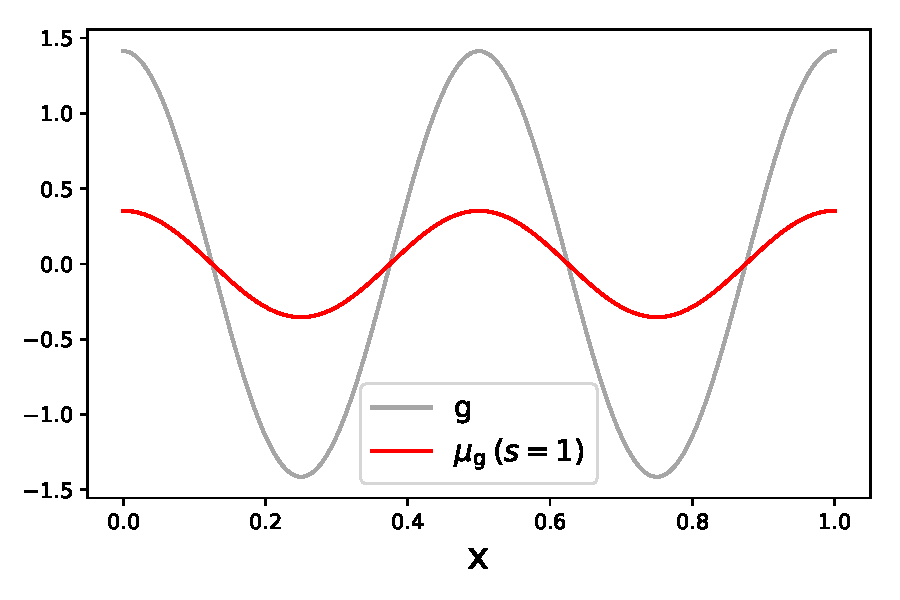
\includegraphics[width= 0.28\textwidth]{img/mean_element/Sobolev/mean_element_cos_ko_1.pdf}~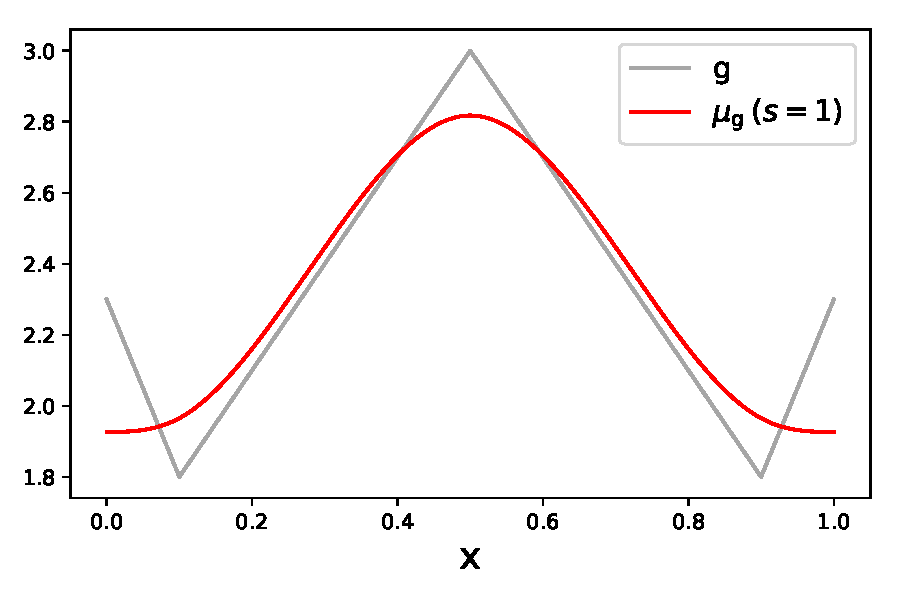
\includegraphics[width= 0.28\textwidth]{img/mean_element/Sobolev/mean_element_saw_ko_1.pdf}~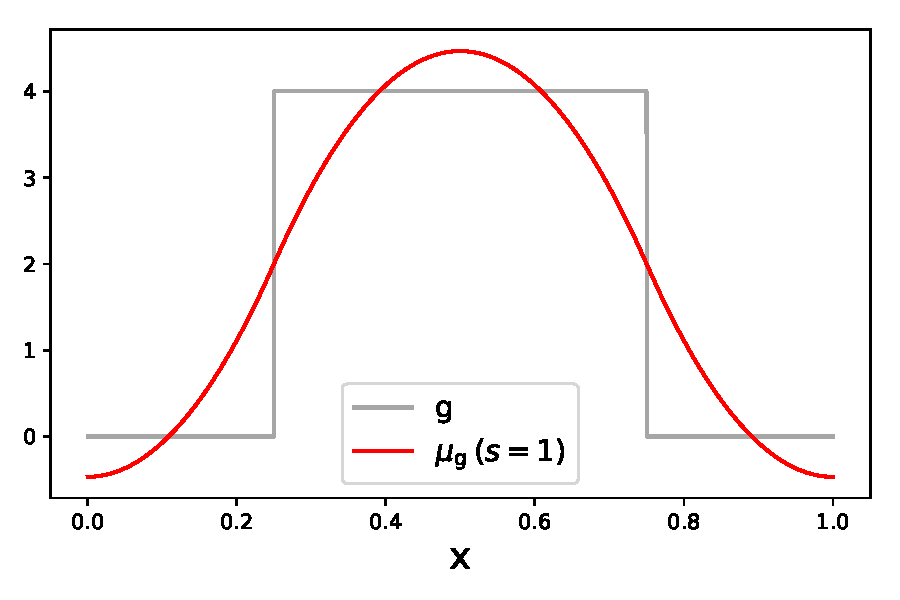
\includegraphics[width= 0.28\textwidth]{img/mean_element/Sobolev/mean_element_step_ko_1.pdf}\\
\caption{$\mu_{g}$ in the periodic Sobolev space for three different $g$.
\label{fig:mean_element}}
\end{figure}
 % The approaches described in this section differ by their choice of nodes and weights.

Now for $d \in \mathbb{N}^{*}$ and $\mathcal{X} = [0,1]^{d}$ and $\mathrm{d}\omega$ is the uniform measure on $\mathcal{X}$. 

The Korobov space of order $s$ is the tensor product of $d$ copies of the Sobolev space $\mathcal{F}_{s}$:
\begin{equation}
\mathcal{K}_{d,s} = \{ f \in \mathbb{L}_{2}(\mathrm{d}\omega), \: f = \prod\limits_{\delta \in [d]} f_{\delta}, \: f_{\delta} \in \mathcal{F}_{s} \}.
\end{equation}

$\mathcal{K}_{d,s}$ is the RKHS corresponding to the tensor product of $d$ copies of the periodic Sobolev kernel

\begin{equation}
\forall x,y \in [0,1]^{d}, \:\: k_{d,s}(x,y) = \prod\limits_{\delta \in [d]}k_{s}(x_{\delta},y_{\delta}).
\end{equation}


\paragraph{Anchored kernels}

\begin{equation}
k_{QMC}(\bm{x},\bm{y}) = \prod\limits_{\delta \in [d]} (2-\min(x_{\delta},y_{\delta})).
\end{equation}


% \paragraph{Kernel quadrature and QMC}



% We recall in the following the aspects shared between kernel quadrature and quasi-Monte Carlo methods and we show the potential benefits of optimal kernel quadrature rules. 

\subsubsection{The link with Bayesian quadrature}
\label{subsec:bayesian_quadrature}
\emph{Bayesian Quadrature} initially \citep{Lar72} considered a fixed set of nodes and put a Gaussian process prior on the integrand $f$. Then, the weights were chosen to minimize the posterior variance of the integral of $f$. If the kernel of the Gaussian process is chosen to be $k$, this amounts to minimizing the RHS of \eqref{eq:integral_bound_mean_element}. The case of the Gaussian reference measure was later investigated in detail \citep{Hag91}, while parametric integrands were considered in \citep{Min00}.
\subsubsection{Design selection for the optimal kernel quadrature}
\label{subsec:okq_analysis_paradigm}
\subsubsection{Ridge leverage score quadrature}
\label{subsec:okq_algebraic_paradigm}

The work of \cite{Bac17} highlights the fundamental role played by the spectral decomposition of the operator $\bm{\Sigma}$ in designing and analyzing kernel quadrature rules.
In fact, the author proposed to sample the nodes $(x_j)$ i.i.d. from some proposal distribution $q$, and then take the vector of weights $\bm{w}$ to be the vector $\bm{w}_{\lambda}$ that solve the optimization problem
\begin{equation}\label{eq:reg_kernel_opt_problem}
\min\limits_{w \in \mathbb{R}^{N}} \Big\| \mu_{g} - \sum\limits_{j \in [N]} \frac{w_{j}}{q(x_{j})^{1/2}} k(x_{j},.) \Big\|_{\mathcal{F}}^{2} + \lambda N \|w\|_{2}^{2},
\end{equation}
for some regularization parameter $\lambda>0$. 

% The idea of the author was to make use of the spectral decomposition of the integral operator $\bm{\Sigma}: \mathbb{L}_{2}(\mathrm{d}\omega) \rightarrow \mathbb{L}_{2}(\mathrm{d}\omega)$ defined by
% \begin{equation}
% \bm{\Sigma} f (\cdot) = \int_{\mathcal{X}} k(\cdot,y)f(y) \mathrm{d}\omega(y), \quad f \in \mathbb{L}_{2}(\mathrm{d}\omega),
% \end{equation}
% in the design and the analysis of the worst integration error of the quadrature. 

% In fact, 

% Finally, we note that Proposition~\ref{p:bach} highlights the fundamental role played by the spectral decomposition of the operator $\bm{\Sigma}$ in designing and analyzing kernel quadrature rules.
 

% In order to understand the importance of the spectral decomposition of $\bm{\Sigma}$ in the design of the quadrature, 

Within this analysis, any proposal distribution $q$, with $q>0$, could be used to sample $N$ i.i.d. nodes that constitutes the design $\bm{x}$: this follows from the following result.

\begin{proposition}[Proposition 1 in \cite{Bac17}]
\label{p:bach_general_proposal}
Let $\delta \in ]0,1]$, and denote
\begin{equation}
d_{\max}(q,\lambda) = \sup\limits_{x \in \X} \frac{1}{q(x)} \langle k(x,.), (\bm{\Sigma}+\lambda \mathbb{I}_{\mathbb{L}_{2}(\mathrm{d}\omega)})^{-1}k(x,.) \rangle_{\mathbb{L}_{2}(\mathrm{d}\omega)}.
\end{equation}
Assume that $N \geq 5 d_{\max}(q,\lambda) \log(16 d_{\max}(q,\lambda) / \delta)$, then
\begin{equation}
\Prb \bigg( \sup\limits_{\|g\|_{\mathrm{d}\omega} \leq 1} \inf\limits_{\|\bm{w}\|^{2}\leq \frac{4}{N}} \Big\| \mu_{g} - \sum\limits_{j \in [N]} \frac{w_{j}}{q_\lambda(x_{j})^{1/2}} k(x_{j},.)\Big\|_{\mathcal{F}}^{2} \leq 4\lambda \bigg) \geq 1- \delta .
\end{equation}
\end{proposition}



In other words, Proposition~\ref{p:bach_general_proposal} gives a uniform  control on the approximation error $\mu_{g}$ by the subspace spanned by the $k(x_{j},.)$ for $g$ belonging to the unit ball of $\mathbb{L}_{2}(\mathrm{d}\omega)$, where the $(x_{j})$ are sampled i.i.d. from $q$. The required number of nodes is equal to $\mathcal{O}(d_{\max}(q,\lambda)\log d_{\max}(q,\lambda))$ for a given approximation error $\lambda$. This bound is relevant if an upper bound of the \emph{maximal ridge leverage score} $d_{\max}(q,\lambda)$ is known. This is possible in some cases; yet in general this quantity is hard to control. Nevertheless, the author showed that one may use a specific choice of $q$, namely the ridge leverage score distribution $q_{\lambda}^{*}$ defined as

\begin{equation}
q_{\lambda}^*(x) \propto \langle k(x,.), \bm{\Sigma}^{-1/2}(\bm{\Sigma}+ \lambda \mathbb{I}_{\mathbb{L}_{2}(\mathrm{d}\omega)})^{-1}\bm{\Sigma}^{-1/2} k(x,.) \rangle_{\mathbb{L}_{2}(\mathrm{d}\omega)} = \sum\limits_{m \in \mathbb{N}^{*}} \frac{\sigma_{m}}{\sigma_{m}+\lambda} e_{m}(x)^{2}.
\label{e:proposalBach}
\end{equation}
Indeed, for this specific choice of $q$
\begin{align}
d_{\max}(q_{\lambda}^{*},\lambda) & = \int_{\X}\langle k(x,.), \bm{\Sigma}^{-1/2}(\bm{\Sigma}+ \lambda \mathbb{I}_{\mathbb{L}_{2}(\mathrm{d}\omega)})^{-1}\bm{\Sigma}^{-1/2} k(x,.) \rangle_{\mathbb{L}_{2}(\mathrm{d}\omega)} \mathrm{d}\omega(x) \nonumber \\
& = \sum\limits_{m \in \mathbb{N}^{*}} \frac{\sigma_{m}}{\sigma_{m}+\lambda} \nonumber\\
& =\Tr \bm{\Sigma}(\bm{\Sigma} + \lambda \bm{I})^{-1}  ,
\end{align}
and the quantity 
\begin{equation}
d_\lambda = \Tr \bm{\Sigma}(\bm{\Sigma} + \lambda \bm{I})^{-1},
\end{equation}
is called the \emph{effective degree of freedom}. This quantity is more amenable to analysis as it depends only on $\lambda$ and on the eigenvalues of $\bm{\Sigma}$.
An instantiation of Proposition~\ref{p:bach_general_proposal} using the ridge leverage score distribution $q_{\lambda}^{*}$ yields the following result.

\begin{proposition}[Proposition 2 in \cite{Bac17}]
\label{p:bach}
Let $\delta \in ]0,1]$. Assume that $N \geq 5 d_\lambda \log(16 d_\lambda / \delta)$, then
\begin{equation}
\Prb \bigg( \sup\limits_{\|g\|_{\mathrm{d}\omega} \leq 1} \inf\limits_{\|\bm{w}\|^{2}\leq \frac{4}{N}} \Big\| \mu_{g} - \sum\limits_{j \in [N]} \frac{w_{j}}{q_\lambda(x_{j})^{1/2}} k(x_{j},.)\Big\|_{\mathcal{F}}^{2} \leq 4\lambda \bigg) \geq 1- \delta .
\end{equation}
\end{proposition}

Now, for fixed $\lambda$, the approximation error in Proposition~\ref{p:bach} does not go to zero when $N$ increases. One theoretical  workaround is to make $\lambda=\lambda(N)$ decrease with $N$. However, the coupling of $N$ and $\lambda$ through $d_\lambda$ makes it very intricate to derive a convergence rate from Proposition~\ref{p:bach}.
Moreover, the optimal density $q_{\lambda}^*$ is in general only available as the limit \eqref{e:proposalBach}, which makes sampling and evaluation difficult. 


\subsection{Projection DPP for kernel quadrature}
% \subsubsection{The proposed algorithm}

We follow in the footsteps of \cite{Bac17}, as reviewed in Section~\ref{s:bach}, but using a projection DPP rather than independent sampling to obtain the nodes.
In a nutshell, we consider nodes $(x_{j})_{j \in [N]}$ that are drawn from the projection DPP with reference measure $\mathrm{d}\omega$ and repulsion kernel
\begin{equation}
  \KDPP(x,y) = \sum\limits_{n \in [N]} e_{n}(x)e_{n}(y),
  \label{e:kernel}
\end{equation}
where we recall that $(e_n)$ are the normalized eigenfunctions of the integral operator $\bm{\Sigma}$.
\subsubsection{The theoretical guarantees}


%
The weights $\bm{w}$ are obtained by solving the optimization problem
\begin{equation}\label{eq:unreg_opt_problem}
\min\limits_{w \in \mathbb{R}^{N}} \| \mu_{g} - \bm{\Phi} \bm{w} \|_{\mathcal{F}}^{2},
%\quad \text{ where } \quad
%\bm{\Phi}:(w_{j})_{j \in [N]} \mapsto \sum\limits_{j \in [N]} w_{j} k(x_{j},.).
\end{equation}
where
\begin{equation}
	\bm{\Phi}:(w_{j})_{j \in [N]} \mapsto \sum_{j \in [N]} w_{j} k(x_{j},.)
\end{equation}
 is the reconstruction operator\footnote{The reconstruction operator $\bm{\Phi}$ depends on the nodes $x_{j}$, although our notation doesn't reflect it for simplicity.}. In Section~\ref{subsec:unreg_opt_problem} we prove that \eqref{eq:unreg_opt_problem} almost surely has a unique solution $\hat{\bm{w}}$ and state our main result, an upper bound on the expected approximation error $\|\mu_{g} - \bm{\Phi}\hat{\bm{w}}\|^{2}_{\mathcal{F}}$ under the proposed Projection DPP. The sketch of the proofs of the main results are given in Section~\ref{subsec:dpp_quadrature_error_weak} and  Section~\ref{subsec:dpp_quadrature_error_strong}.

 %%%%%%%%
\subsubsection{Main results}
\label{subsec:unreg_opt_problem}
Assuming that nodes $(x_{j})_{j \in [N]}$ are known, we first need to solve the optimization problem \eqref{eq:unreg_opt_problem} that relates to problem~\eqref{eq:reg_kernel_opt_problem} without regularization ($\lambda = 0$).
%
Let $\bm{x} = (x_{1}, \dots, x_{N}) \in \mathcal{X}^{N}$, then
% using the fact that $\langle \mu, k(x_{i},.) \rangle_{\mathcal{F}} = \mu(x_{i})$:
% \begin{align}
% \| \mu - \bm{\Phi} \bm{w} \|_{\mathcal{F}}^{2} & = \|\mu\|_{\mathcal{F}}^{2} - 2 \sum\limits_{i \in [N]} w_{i} \mu(x_{i}) + \sum\limits_{1\leq i,j \leq N}w_{i}w_{j}k(x_{i},x_{j})\\
% &= \|\mu\|_{\mathcal{F}}^{2} - 2 \bm{w}^{\Tran} \mu(x_{i})_{i \in [N]} + \bm{w}^{\Tran} \bm{K} \bm{w}.
% \end{align}
\begin{equation}
\| \mu_{g} - \bm{\Phi} \bm{w} \|_{\mathcal{F}}^{2} = \|\mu_{g}\|_{\mathcal{F}}^{2} - 2 \bm{w}^{\Tran} \mu_{g}(x_{j})_{j \in [N]} + \bm{w}^{\Tran} \bm{K}(\bm{x}) \bm{w},
\label{e:quadratic}
\end{equation}
where $\bm{K}(\bm{x}) = (k(x_{i},x_{j}))_{i,j \in [N]}$. The right-hand side of \eqref{e:quadratic} is quadratic in $\bm{w}$, so that the optimization problem \eqref{eq:unreg_opt_problem}
% \begin{equation}
%   \label{e:optimization}
% \min\limits_{w \in \mathbb{R}^{N}} \| \mu_{g} - \bm{\Phi} \bm{w} \|_{\mathcal{F}}^{2}
% \end{equation}
admits a unique solution $\hat{\bm{w}}$ if and only if $\bm{K}(\bm{x})$ is invertible. In this case, the solution is given by $\hat{\bm{w}} = \bm{K}(\bm{x})^{-1}\mu_{g}(x_{j})_{j \in [N]}$. A sufficient condition for the invertibility of $\bm{K}(\bm{x})$ is given in the following proposition.
%%% PROPOSITION
% Let $\{x_{1}, \dots, x_{N}\} \in \mathcal{X}^{N}$ be such that
\begin{proposition}\label{prop:K_N_non_singular}
Assume that the matrix
$\bm{E}(\bm{x}) = (e_{i}(x_{j}))_{ i,j \in [N]}$ is invertible, then $\bm{K}(\bm{x})$ is invertible.
\end{proposition}
%%%
The proof of Proposition~\ref{prop:K_N_non_singular} is given in Appendix~\ref{app:K_N_non_singular}.
Since the pdf \eqref{eq:pdpp_definition} of the projection DPP with kernel \eqref{e:kernel} is proportional to $\Det^2\bm{E}(\bm{x})$, the following corollary immediately follows.

\begin{corollary}
  Let $\bm{x} = \{x_{1}, \dots , x_{N}\}$ be a projection DPP with reference measure $\mathrm{d}\omega$ and kernel $\KDPP$ defined in \eqref{e:kernel}. Then $\bm{K}(\bm{x})$ is a.s. invertible, so that \eqref{eq:unreg_opt_problem} has unique solution $\hat{\bm{w}} = \bm{K}(\bm{x})^{-1}\mu_{g}(x_{j})_{j \in [N]}$ a.s.
\label{c:regularization}
\end{corollary}
We now give our main result that uses nodes $(x_{j})_{j \in [N]}$ drawn from a well-chosen projection DPP.
%%% THEOREM
\begin{theorem}\label{thm:main_theorem}
Let $\bm{x} = \{x_{1}, \dots , x_{N}\}$ be a projection DPP with reference measure $\mathrm{d}\omega$ and kernel \eqref{e:kernel}. Let $\hat{\bm{w}}$ be the unique solution to \eqref{eq:unreg_opt_problem} and define $\displaystyle \|g\|_{\mathrm{d}\omega,1} = \sum\limits_{n \in [N]} |\langle e_{n},g \rangle_{d\omega}|$. Assume that $\|g\|_{\mathrm{d}\omega} \leq 1$ and define $r_{N} = \sum\limits_{m \geq N+1} \sigma_{m}$, then
\begin{equation}\label{eq:main_result}
\EX_{\DPP} \|\mu_{g} - \bm{\Phi}\hat{\bm{w}}\|_{\mathcal{F}}^{2}  \leq
2\sigma_{N+1} +2\|g\|_{\mathrm{d}\omega,1}^{2}\left(   N r_{N} + \sum\limits_{\ell =2}^{N} \frac{\sigma_{1}}{\ell!^{2}}\left(\frac{Nr_{N}}{\sigma_{1}}\right)^{\ell} \right).
\end{equation}
%with
%\begin{equation}
%	\label{eq:def_rN}
%	r_{N} = \sum\limits_{m \geq N+1} \sigma_{m}.
%\end{equation}
\end{theorem}
%%%
In particular, if $Nr_{N} = o(1)$, then the right-hand side of \eqref{eq:main_result} is $N r_{N} + o(N r_{N})$. For example, take $\mathcal{X} = [0,1]$, $\mathrm{d}\omega$ the uniform measure on $\mathcal{X}$, and $\mathcal{F}$ the $s$-Sobolev space, then $\sigma_{m} = m^{-2s}$ \cite{BeTh11}. Now, if $s > 1$, the expected worst case quadrature error is bounded by $Nr_{N} = \mathcal{O}(N^{2-2s}) = o(1)$. Another example is the case of the Gaussian measure on $\mathcal{X} = \mathbb{R}$, with the Gaussian kernel. In this case $\sigma_{m} = \beta \alpha^{m}$ with $0 < \alpha < 1$ and $\beta >0$ \cite{RaWi06} so that $Nr_{N} = N\frac{\beta}{1-\alpha}\alpha^{N+1}=  o(1)$.
% $\mathrm{d}\omega_{\nu}(x) = (2\pi\nu^{2})^{-1/2}e^{-\frac{1}{2\nu^{2}}x^{2}}$
% $k_{\gamma}(x,y) = \exp[-(x-y)^{2}/2\gamma^{2}]$


% \footnote{$\alpha_{\nu,\gamma} = \frac{1}{1+\frac{1}{2}\rho^{2}+\sqrt{\rho^{2}+\frac{1}{4}\rho^{4}}}$ and $\beta_{\nu,\gamma} = \sqrt{\frac{2}{1+\frac{1}{\rho}+\sqrt{1+2\frac{1}{\rho}}}}$, where $\rho = \frac{\gamma}{\nu}$ \cite{RaWi06} .}
We have assumed that $\mathcal{F}$ is dense in $\mathbb{L}_{2}(\mathrm{d}\omega)$ but Theorem~\ref{thm:main_theorem} is valid also when $\mathcal{F}$ is finite-dimensional. In this case, denote $N_{0} = \dim \mathcal{F}$. Then, for $n > N_{0}$, $\sigma_{n} = 0$ and $r_{N_{0}} = 0$, so that \eqref{eq:main_result} implies
\begin{equation}
  \| \mu_{g} - \bm{\Phi}\hat{\bm{w}}\|_{\mathcal{F}}^{2} = 0 \:\: \text{a.s.}
\end{equation}
This compares favourably with herding, for instance, which comes with a rate in $\mathcal{O}(\frac{1}{N})$ for the quadrature based on herding with uniform weights \cite{BaLaOb12,ChWeSm10}.

The constant $\|g\|_{\mathrm{d}\omega,1}$ in $\eqref{eq:main_result}$ is the $\ell_1$ norm of the coefficients of projection of $g$ onto $\Span(e_{n})_{n \in [N]}$ in $\mathbb{L}_{2}(\mathrm{d}\omega)$. For example, for $g = e_{n}$, $\|g\|_{\mathrm{d}\omega,1} = 1$ if $n \in [N]$ and $\|g\|_{\mathrm{d}\omega,1} = 0$ if $n \geq N+1$. In the worst case, $\|g\|_{\mathrm{d}\omega,1} \leq \sqrt{N} \|g\|_{\mathrm{d}\omega} \leq \sqrt{N}$.
% \begin{equation}\label{eq:l1_worst_case}
% .\leq \sqrt{N} \sqrt{\sum\limits_{n \in [N]} \langle g, e_{n} \rangle_{\mathrm{d}\omega}^{2}}
% \end{equation}
Thus, we can obtain a uniform bound for $\|g\|_{\mathrm{d}\omega}\leq 1$ in the spirit of Proposition~\ref{p:bach}, but with a supplementary factor $N$ in the upper bound in \eqref{eq:main_result}.
% \paragraph{The Gaussian kernel}
% Let,
% \begin{equation}
% k(x,y) = e^{-\frac{(x-y)^{2}}{2a^{2}}},
% \end{equation}
% with
% \begin{equation}
% \mathrm{d}\omega(x) = \frac{1}{\sqrt 2 \sigma}e^{-\frac{x^{2}}{\sigma^2}},
% \end{equation}
% then \cite{Ras03}
% \begin{equation}
% \sigma_{m} = A B^{m},
% \end{equation}
% and
% \begin{equation}
% e_{m} = e^{-(c-a)x^{2}}H_{m}(\sqrt{2c}x).
% \end{equation}

Since the publication of [??], we obtained two refinements of Theorem~\ref{thm:main_theorem}. We report these results in the following Theorem.

\begin{theorem}\label{thm:main_theorem_refined}
Let $\bm{x} = \{x_{1}, \dots , x_{N}\}$ be a projection DPP with reference measure $\mathrm{d}\omega$ and kernel \eqref{e:kernel}. Let $\hat{\bm{w}}$ be the unique solution to \eqref{eq:unreg_opt_problem}. Assume that $\|g\|_{\mathrm{d}\omega} \leq 1$ and define $r_{N} = \sum\limits_{m \geq N+1} \sigma_{m}$, then
\begin{equation}\label{eq:main_result_refined}
\EX_{\DPP} \sup\limits_{\|g\|_{\mathrm{d}\omega} \leq 1}\|\mu_{g} - \bm{\Phi}\hat{\bm{w}}\|_{\mathcal{F}}^{2}  \leq 4 Nr_{N}.
\end{equation}
Moreover, if $g = e_{n}$ for some $m \in \Ns$, then
\begin{equation}\label{eq:main_result_refined_eigfunction}
\EX_{\DPP} \|\mu_{g} - \bm{\Phi}\hat{\bm{w}}\|_{\mathcal{F}}^{2}  \leq r_{N}.
\end{equation}
%with
%\begin{equation}
%	\label{eq:def_rN}
%	r_{N} = \sum\limits_{m \geq N+1} \sigma_{m}.
%\end{equation}
\end{theorem}

Of course, the results in Theorem~\ref{thm:main_theorem_refined} are stronger compared to the ones in Theorem~\ref{thm:main_theorem}. Yet, we think that the proof of Theorem~\ref{thm:main_theorem_refined} will become clearer if we recall the proof of Theorem~\ref{thm:main_theorem} and the intuitions behind. Section~\ref{subsec:dpp_quadrature_error_weak} contains the sketch of the proof of the weak version of our results, while Section~\ref{subsec:dpp_quadrature_error_strong} contains the sketch of the proof of the strong version of our results.



\subsubsection{Bounding the approximation error under the DPP: the weak version}
\label{subsec:dpp_quadrature_error_weak}

In this section, we give the skeleton of the proof of Theorem~\ref{thm:main_theorem}, referring to the appendices for technical details. The proof is in two steps. First, we give an upper bound for the approximation error $\|\mu_{g} - \bm{\Phi}\hat{\bm{w}}\|^{2}_{\mathcal{F}}$ that involves the maximal principal angle between the functional subspaces of $\mathcal{F}$
$$\mathcal{E}_N^{\mathcal{F}} = \Span(e_{n}^{\mathcal{F}})_{n \in [N]} \quad\text{ and }\quad \mathcal{T}(\bm{x}) = \Span(k(x_{j},.))_{j \in [N]}.$$
The second step consists in developing the expectation of the bound under the projection DPP in a similar fashion as in Chapter ??: projection DPPs allow closed form expressions for the expectation of some trigonometric functions of the principal angles.

As for now, we recall some properties of the principal angles between subspaces of a Hilbert space and we give the corresponding instantiation of these results when the Hilbert space is $\F$.
 % and Appendix~\ref{app:geometric_intuition} for the geometric intuition behind the proof



\paragraph{Principal angles between subspaces in a Hilbert space}
\label{subsec:principalangles}
We recall in this section the definition of principal angles between subspaces in Hilbert spaces and connect them to the determinant of the Gramian matrix of their orthonormal bases.

%%% PROPOSITION

\begin{proposition}\label{prop:cos_between_subspaces}
Let $\mathcal{H}$ be a Hilbert space. Let $\mathcal{P}_{1}$ and $\mathcal{P}_{2}$ be two finite-dimensional subspaces of $\mathcal{H}$ with $N = \dim \mathcal{P}_{1} = \dim \mathcal{P}_{2}$. Denote $\bm{\Pi}_{\mathcal{P}_{1}}$ and $\bm{\Pi}_{\mathcal{P}_{2}}$ the orthogonal projections of $\mathcal{H}$ onto these two subspaces. There exist two orthonormal bases for $\mathcal{P}_{1}$ and $\mathcal{P}_{2}$ denoted $(\bm{v}_{i}^{1})_{i \in [N]}$ and $(\bm{v}_{i}^{2})_{i \in [N]}$, and a set of angles $\theta_{i}(\mathcal{P}_{1},\mathcal{P}_{2}) \in [0,\frac{\pi}{2}]$ such that
\begin{equation}
\cos \theta_{N}(\mathcal{P}_{1},\mathcal{P}_{2}) \leq \dots \leq \cos \theta_{1}(\mathcal{P}_{1},\mathcal{P}_{2}) ,
\end{equation}


and for $i \in [1,...,N]$
\begin{equation}
\langle \bm{v}_{i}^{1}, \bm{v}_{i}^{2} \rangle_{\mathcal{H}} = \cos \theta_{i}(\mathcal{P}_{1},\mathcal{P}_{2}),
\end{equation}
and
\begin{equation}\label{eq:principal_vectors_projection_relationship}
 \bm{\Pi}_{\mathcal{P}_{1}}\bm{v}_{i}^{2} = \cos \theta_{i}(\mathcal{P}_{1},\mathcal{P}_{2}) \bm{v}_{i}^{1},
\end{equation}
and
\begin{equation}
 \bm{\Pi}_{\mathcal{P}_{2}}\bm{v}_{i}^{1} = \cos \theta_{i}(\mathcal{P}_{1},\mathcal{P}_{2}) \bm{v}_{i}^{2}.
\end{equation}
In particular
\begin{equation}\label{eq:costhetaN}
\cos \theta_{N}(\mathcal{P}_{1},\mathcal{P}_{2}) = \inf\limits_{\bm{v} \in \mathcal{P}_{1},\|\bm{v}\|_{\mathcal{H}} = 1} \|\bm{\Pi}_{\mathcal{P}_{2}}\bm{v}\|_{\mathcal{H}}.
\end{equation}
\end{proposition}
We refer to \cite{GoVa12} for the proof when $\mathcal{H}$ is finite-dimensional. We give a proof in the general case in ??; see also \cite{DaKa70}.
% \begin{proof}
% Assume that $\mathcal{P}_{1} \cap \mathcal{P}_{2} \neq \{\bm{0} \}$ and put $p = \dim \mathcal{P}_{1} \cap \mathcal{P}_{2}$. Let $(\bm{v}^{1}_{i})_{i \in [p]} = (\bm{v}^{2}_{i})_{i \in [p]}$ an orthonormal basis of $\mathcal{P}_{1} \cap \mathcal{P}_{2}$, and denote for $i \in [p], \: \theta_{i} = 0$. If $p = N$, $\mathcal{P}_{1} = \mathcal{P}_{2} = \mathcal{P}_{1} \cap \mathcal{P}_{2}$ and $\theta_{1} = \dots = \theta_{N} = 0$. If not, the subspace $\mathcal{P}_{1} \cap \mathcal{P}_{2}$ is strictly included in $\mathcal{P}_{1}$ and $\mathcal{P}_{2}$ such that the subspaces $\mathcal{P}_{1} \cap (\mathcal{P}_{1} \cap \mathcal{P}_{2})^{\perp}$ and $\mathcal{P}_{2} \cap (\mathcal{P}_{1} \cap \mathcal{P}_{2})^{\perp}$ are non-trivial. Now, let
% \begin{equation}
% \mathcal{P}_{1}^{0} = \mathcal{P}_{1} \cap (\mathcal{P}_{1} \cap \mathcal{P}_{2})^{\perp},
% \end{equation}
% and
% \begin{equation}
% \mathcal{P}_{2}^{0} = \mathcal{P}_{2} \cap (\mathcal{P}_{1} \cap \mathcal{P}_{2})^{\perp}.
% \end{equation}
%
% Define $(\bm{v}^{1}_{p +1}, \bm{v}^{2}_{p +1}) \in \mathcal{P}_{1}^{0} \times \mathcal{P}_{2}^{0}$ such that
% \begin{equation}
% \langle \bm{v}^{1}_{p +1}, \bm{v}^{2}_{p +1} \rangle_{\mathcal{H}} = \max\limits_{\substack{\bm{v}^{1} \in \mathcal{P}_{1}^{0},\bm{v}^{2} \in \mathcal{P}_{2}^{0}\\ \|\bm{v}^{1}\| = 1, \|\bm{v}^{2}\| = 1}} \langle \bm{v}^{1}, \bm{v}^{2} \rangle_{\mathcal{H}},
% \end{equation}
% and put $\theta_{p+1} \in [0, \frac{\pi}{2}]$ such that $\cos \theta_{p+1} = \langle \bm{v}^{1}_{p +1}, \bm{v}^{2}_{p +1} \rangle_{\mathcal{H}}$. Now if $p+1 < N$, define for $\ell \in [N-p]$ recursively the subspaces
% \begin{equation}
% \mathcal{P}_{1}^{\ell} = \mathcal{P}_{1}^{\ell-1} \cap \bm{v}^{1 \perp}_{p+\ell},
% \end{equation}
% and
% \begin{equation}
% \mathcal{P}_{2}^{\ell} = \mathcal{P}_{2}^{\ell-1} \cap \bm{v}^{2 \perp}_{p+\ell},
% \end{equation}
% along with  $(\bm{v}^{1}_{p+\ell+1},\bm{v}^{2}_{p+\ell+1}) \in \mathcal{P}_{1}^{\ell} \times \mathcal{P}_{2}^{\ell}$ such that
% \begin{equation}
% \langle \bm{v}^{1}_{p +\ell+1}, \bm{v}^{2}_{p +\ell+1} \rangle_{\mathcal{H}} = \max\limits_{\substack{\bm{v}^{1} \in \mathcal{P}_{1}^{\ell},\bm{v}^{2} \in \mathcal{P}_{2}^{\ell}\\ \|\bm{v}^{1}\| = 1, \|\bm{v}^{2}\| = 1}} \langle \bm{u}, \bm{v} \rangle_{\mathcal{H}} ,
% \end{equation}
% and let $\theta_{p +\ell+1} \in [0, \frac{\pi}{2}]$ such that $\langle \bm{v}^{1}_{p +\ell+1}, \bm{v}^{2}_{p +\ell+1} \rangle_{\mathcal{H}} = \cos \theta_{p +\ell+1}$. By construction $(\bm{v}^{1}_{\ell})_{\ell \in [N]}$ is an orthonormal basis of $\mathcal{P}_{1}$ and $(\bm{v}^{2}_{\ell})_{\ell \in [N]}$ is an orthonormal basis of $\mathcal{P}_{2}$ such that
% \begin{equation}
% \forall i \in [N], \: \langle \bm{v}^{1}_{i}, \bm{v}^{2}_{i} \rangle_{\mathcal{H}} = \cos \theta_{i}.
% \end{equation}
% \end{proof}
The following result shows that the principal angles are somewhat independent of the choice of orthonormal bases. It can be found in \cite{BjGo73,MiBe92} for the finite dimensional case. We give here the proof for the general case, for the sake of completeness.
\begin{corollary}\label{cor:cos_det_relationship}
Let $(\bm{w}^{1}_{i})_{i \in [N]}$ be any orthonormal basis of $\mathcal{P}_{1}$ and $(\bm{w}^{2}_{i})_{i \in [N]}$ be any orthonormal basis of $\mathcal{P}_{2}$, and let $\bm{W} = (\langle \bm{w}^{1}_{i},\bm{w}^{2}_{j} \rangle_{\mathcal{H}})_{1\leq i,j \leq N}$ and $\bm{G} = \bm{W}\bm{W}^{\Tran}$. Then
the eigenvalues of $\bm{G}$ are the $\cos^{2} \theta_{i}(\mathcal{P}_{1},\mathcal{P}_{2})$. In particular, $\Det^{2} \bm{W} = \Det \bm{G} =  \prod\limits_{i \in [N]} \cos^{2} \theta_{i}(\mathcal{P}_{1},\mathcal{P}_{2})$.
\end{corollary}

\begin{proof}
Let $(\bm{v}^{i}_{i})_{i \in [N]}$, $i\in\{1,2\}$, be the bases of Proposition~\ref{prop:cos_between_subspaces}. Let $\bm{U}^{1} \in \mathbb{O}_{N}(\mathbb{R})$ be such that
\begin{equation}
\forall i \in [N], \: \bm{w}^{1}_{i} = \sum\limits_{j \in [N]} u^{1}_{i,j} \bm{v}^{1}_{j}.
\end{equation}
Similarly, there exists a matrix $\bm{U}^{2} \in \mathbb{O}_{N}(\mathbb{R})$ such that
\begin{equation}
\forall i \in [N], \: \bm{w}^{2}_{i} = \sum\limits_{j \in [N]} u^{2}_{i,j} \bm{v}^{2}_{j}.
\end{equation}
This implies that
\begin{equation}
\bm{W} = \bm{U}^{1}\bm{V}\bm{U}^{2 \Tran},
\end{equation}
where $\displaystyle \bm{V} = (\langle \bm{v}^{1}_{i}, \bm{v}^{2}_{j} \rangle_{\mathcal{H}})_{1 \leq i,j \leq N}$. Then
\begin{equation}
\bm{G} = \bm{W}\bm{W}^{\Tran} = \bm{U}^{1}\bm{V}\bm{V}^{\Tran}\bm{U}^{1 \Tran}.
\end{equation}
Thus the eigenvalues of $\bm{G}$ are the eigenvalues of $\bm{V}\bm{V}^{\Tran}$. By Proposition~\ref{prop:cos_between_subspaces}, the diagonal elements of $\bm{V}$ are
\begin{equation}\label{eq:diagonal_of_V}
v_{i,i} = \langle \bm{v}^{1}_{i}, \bm{v}^{2}_{i} \rangle_{\mathcal{H}} = \cos \theta_{i}(\mathcal{P}_{1},\mathcal{P}_{2}).
\end{equation}
We finish the proof by showing that the anti-diagonal elements satisfy
\begin{equation}\label{eq:anti_diagonal_of_V}
v_{i,j} = \langle \bm{v}^{1}_{i}, \bm{v}^{2}_{j} \rangle_{\mathcal{H}} = 0.
\end{equation}
By \eqref{eq:principal_vectors_projection_relationship},
\begin{equation}
\forall i \in [N], \:\sum\limits_{j \in [N]} \langle \bm{v}_{i}^{2}, \bm{v}_{j}^{1}\rangle_{\mathcal{H}}^{2} = \|\bm{\Pi}_{\mathcal{P}_{1}}\bm{v}_{i}^{2}\|_{\mathcal{H}}^{2} = \cos^{2} \theta_{i}(\mathcal{P}_{1},\mathcal{P}_{2}).
\end{equation}
Then
\begin{equation}
 \sum\limits_{i \in [N]}\sum\limits_{j \in [N]} \langle \bm{v}_{i}^{2}, \bm{v}_{j}^{1}\rangle_{\mathcal{H}}^{2} = \sum\limits_{i \in [N]} \cos^{2} \theta_{i}(\mathcal{P}_{1},\mathcal{P}_{2}) = \sum\limits_{i \in [N]} \langle \bm{v}_{i}^{2}, \bm{v}_{i}^{1}\rangle_{\mathcal{H}}^{2} .
\end{equation}
Thus
\begin{equation}
\sum\limits_{\substack{i,j \in [N]\\ i \neq j}} \langle \bm{v}_{i}^{2}, \bm{v}_{i}^{1}\rangle_{\mathcal{H}}^{2} = 0 .
\end{equation}
Finally, $\bm{V}$ is a diagonal matrix and the eigenvalues of $\bm{G}$ are the $\cos^{2} \theta_{i}(\mathcal{P}_{1},\mathcal{P}_{2})$.
% For $i \in \{1,2\}$, consider the following operator:
% \begin{equation}
%  \bm{P}_{\mathcal{P}_{i}} =   \left\{
% \begin{array}{ll}
%       \mathbb{R}^{d} \rightarrow  \mathcal{H}& \\
%       \bm{c} \rightarrow \sum\limits_{j \in [N]} c_{j} \bm{u}^{i}_{j} & \\
% \end{array}
% \right. ,
% \end{equation}
% along with its adjoint:
% \begin{equation}
%  \bm{P}_{\mathcal{P}_{i}}^{*} =   \left\{
% \begin{array}{ll}
%       \mathcal{H} \rightarrow  \mathbb{R}^{d}& \\
%       \bm{x} \rightarrow  (\langle \bm{x}, \bm{u}_{j}^{i} \rangle )_{j \in [N]}& \\
% \end{array}
% \right. .
% \end{equation}
% Observe that
% \begin{equation}
% \bm{W} = \bm{P}_{\mathcal{P}_{1}}^{*}\bm{P}_{\mathcal{P}_{2}}
% \end{equation}
% Now, for $j \in [d_1]$,
% \begin{equation}
% \bm{P}_{\mathcal{P}_{2}}^{*}\bm{P}_{\mathcal{P}_{1}} \bm{e}_{j}^{1} = \cos \theta_{j} \bm{e}_{j}^{2}
% \end{equation}
\end{proof}

A simple application of Corollary~\ref{cor:cos_det_relationship}, in the case $\mathcal{H} = \F$, $\mathcal{P}_{1} = \mathcal{E}_{N}^{\F}$ and $\mathcal{P}_{2} = \mathcal{T}(\bm{x})$ leads to the following result.

\begin{lemma}\label{lemma:cos_ratio_det}
Let $\bm{x} =  (x_{1}, \dots , x_{N}) \in \mathcal{X}^{N} $ such that $\Det^{2} \bm{E}(\bm{x}) \neq 0$. Then,
\begin{equation}
\prod\limits_{\ell \in [N]} \frac{1}{\cos^{2} \theta_{\ell} \left(\mathcal{E}^{\mathcal{F}}_{N}, \mathcal{T}(\bm{x}) \right)} = \frac{\Det \bm{K}(\bm{x})}{\Det^{2} \bm{E}^{\mathcal{F}}(\bm{x})}.
\end{equation}
\end{lemma}

\begin{proof}
The condition $\Det^{2} \bm{E}(\bm{x}) \neq 0$ yields by Proposition~\ref{prop:K_N_non_singular} that $\bm{K}(\bm{x})$ is non singular. Thus $\dim \mathcal{T}(\bm{x}) = N$. Let $(t_{i})_{i \in [N]}$ be an orthonormal basis of $\mathcal{T}(\bm{x})$ with respect to $\langle ., . \rangle_{\mathcal{F}}$.
%
Using Corollary~\ref{cor:cos_det_relationship}, and the fact that $(e_{n}^{\mathcal{F}})_{n \in [N]}$ is an orthonormal basis of $\mathcal{E}^{\mathcal{F}}_{N}$ according to $\langle ., . \rangle_{\mathcal{F}}$,
\begin{equation}\label{eq:prod_cos_det_E}
\prod\limits_{\ell \in [N]} \cos^{2} \theta_{\ell} \left(\mathcal{E}^{\mathcal{F}}_{N}, \mathcal{T}(\bm{x}) \right) = \Det^{2} (\langle e_{n}^{\mathcal{F}}, t_{i} \rangle_{\mathcal{F}})_{(n,i) \in [N]\times[N]}.
\end{equation}
Now, write for $i \in [N]$,
\begin{equation}\label{eq:t_as_function_of_kx}
t_{i} = \sum\limits_{j \in [N]} c_{i,j} k(x_{j},.).
\end{equation}
%
Thus
\begin{align}
\langle e_{n}^{\mathcal{F}}, t_{i} \rangle_{\mathcal{F}} = & \sum\limits_{j \in [N]} c_{i,j} \langle e_{n}^{\mathcal{F}}, k(x_{j},.) \rangle_{\mathcal{F}} \\
= &\sum\limits_{j \in [N]} c_{i,j}  e_{n}^{\mathcal{F}}(x_{j}).
\end{align}
%
Then
\begin{equation}
(\langle e_{n}^{\mathcal{F}}, t_{i} \rangle_{\mathcal{F}})_{(n,i) \in [N]\times[N]} = \bm{E}^{\mathcal{F}}(\bm{x}) \bm{C}(\bm{x})^{\Tran} ,
\end{equation}
where
\begin{equation}
\bm{C}(\bm{x}) = (c_{i,j})_{1 \leq i,j \leq N}.
\end{equation}
%
Thus
\begin{equation}\label{eq:AN_times_EN}
\Det^{2} (\langle e_{n}^{\mathcal{F}}, t_{i} \rangle_{\mathcal{F}})_{(n,i) \in [N]\times[N]} = \Det^{2} \bm{C}(\bm{x}) \Det^{2} \bm{E}^{\mathcal{F}}(\bm{x}).
\end{equation}
%%%%
Now, let $\bm{c}_{i}$ the columns of the matrix $\bm{C}(\bm{x})$. $(t_{i})_{i \in [N]}$ is an orthonormal basis of $\mathcal{T}(\bm{x})$ with respect to $\langle .,. \rangle_{\mathcal{F}}$, then by \eqref{eq:t_as_function_of_kx}
\begin{equation}
  \delta_{i,i'} = \langle t_{i}, t_{i'} \rangle_{\mathcal{F}} = \bm{c}_{i}^{\Tran} \bm{K}(\bm{x}) \bm{c}_{i'}  .
\end{equation}
Therefore
\begin{equation}
\bm{C}(\bm{x})^{\Tran} \bm{K}(\bm{x}) \bm{C}(\bm{x}) = \mathbb{I}_{N}.
\end{equation}
Thus
\begin{equation}\label{eq:det_AN_det_KN_relationship}
\Det^{2} \bm{C}(\bm{x}) = \frac{1}{\Det \bm{K}(\bm{x})}.
\end{equation}
Combining \eqref{eq:prod_cos_det_E}, \eqref{eq:AN_times_EN} and \eqref{eq:det_AN_det_KN_relationship} concludes the proof of Lemma~\ref{lemma:cos_ratio_det}:
\begin{equation}
\prod\limits_{\ell \in [N]} \frac{1}{\cos^{2} \theta_{\ell} \left(\mathcal{E}^{\mathcal{F}}_{N}, \mathcal{T}(\bm{x}) \right)} = \frac{\Det \bm{K}(\bm{x})}{\Det^{2} \bm{E}^{\mathcal{F}}(\bm{x})}.
\end{equation}
\end{proof}



\paragraph{Bounding the approximation error using principal angles}
\label{subsec:approximation_error_principal_angle}
 Let $\bm{x} =  (x_{1}, \dots , x_{N}) \in \mathcal{X}^{N} $ be such that $\Det \bm{E}(\bm{x}) \neq 0$. By Proposition~\ref{prop:K_N_non_singular}, $\bm{K}(\bm{x})$ is non singular and $\dim \mathcal{T}(\bm{x}) = N$. The optimal approximation error writes
\begin{equation}
\|\mu_{g} - \bm{\Phi}\hat{\bm{w}}\|^{2}_{\mathcal{F}} =\|\mu_{g} - \bm{\Pi}_{\mathcal{T}(\bm{x})}\mu_{g}\|^{2}_{\mathcal{F}},\label{e:finalTool}
\end{equation}
%  The approximation error writes
% \begin{align}
% \|\mu_{g} - \bm{\Phi}\hat{\bm{w}}\|^{2}_{\mathcal{F}} &= \|\mu_{g} - \bm{\Phi}\bm{K}(\bm{x})^{-1} \mu_{g}(x_{i})_{i \in [N]}\|^{2}_{\mathcal{F}}\\
%  &= \|\mu_{g} - \bm{\Phi}(\bm{\Phi}^{*}\bm{\Phi})^{-1}\bm{\Phi}^{*} \mu_{g} \|^{2}_{\mathcal{F}}\\
% &=\|\mu_{g} - \bm{\Pi}_{\mathcal{T}(\bm{x})}\mu_{g}\|^{2}_{\mathcal{F}},\label{e:finalTool}
% \end{align}
where $\bm{\Pi}_{\mathcal{T}(\bm{x})} = \bm{\Phi}(\bm{\Phi}^{*}\bm{\Phi})^{-1}\bm{\Phi}^{*}$ is the orthogonal projection onto $\mathcal{T}(\bm{x})$ with $\bm{\Phi}^{*}$ the dual\footnote{For $\mu \in \mathcal{F}$,$\bm{\Phi}^{*}\mu = (\mu(x_{j}))_{j \in [N]}$. $\bm{\Phi}^{*}\bm{\Phi}$ is an operator from $\mathbb{R}^{N}$ to $\mathbb{R}^{N}$ that can be identified with $\bm{K}(\bm{x})$.} of $\bm{\Phi}$.

In other words, \eqref{e:finalTool} equates the approximation error to $\|\bm{\Pi}_{\mathcal{T}(\bm{x})^{\perp}}\mu_g\|^{2}_{\mathcal{F}}$, where $\bm{\Pi}_{\mathcal{T}(\bm{x})^{\perp}}$ is the orthogonal projection onto $\mathcal{T}(\bm{x})^{\perp}$.
% \rb{and maybe give a ref on the definition of the projection, since $\Phi$ is an operator}.
Now we have the following lemma.

\begin{lemma}\label{lemma:approximation_error_spectral_bound}
Assume that $\|g\|_{\mathrm{d}\omega} \leq 1$ then $\| \bm{\Sigma}^{-1/2} \mu_{g} \|_{\mathcal{F}} \leq 1$ and
\begin{equation}
	\|\bm{\Pi}_{\mathcal{T}(\bm{x})^{\perp}}\mu_{g}\|^{2}_{\mathcal{F}} \leq 2 \bigg( \sigma_{N+1} + \|g\|_{\mathrm{d}\omega,1}^2  \max\limits_{ n \in [N]} \sigma_{n}\|\bm{\Pi}_{\mathcal{T}(\bm{x})^{\perp}} e_{n}^{\mathcal{F}}\|_{\mathcal{F}}^{2} \bigg) .
\label{e:boundingOrthogonalProjection}
\end{equation}
% with $\displaystyle c(g) = \sum\limits_{n \in [N]} |\langle \bm{\Sigma}^{-1/2} \mu_{g}, e_{n}^{\mathcal{F}} \rangle_{\mathcal{F}}| = \sum\limits_{n \in [N]} |\langle g, e_{n} \rangle_{\mathrm{d}\omega}|$.
\end{lemma}

% \rb{Make this an assumption using begin/end{assumption}, and comment on it, saying what it means and that others used the same.}

Now, to upper bound the right-hand side of \eqref{e:boundingOrthogonalProjection}, we note that $\sigma_{n}\|\bm{\Pi}_{\mathcal{T}(\bm{x})^{\perp}} e_{n}^{\mathcal{F}}\|_{\mathcal{F}}^{2}$ is the product of two terms: $\sigma_{n}$ is a decreasing function of $n$ while $\|\bm{\Pi}_{\mathcal{T}(\bm{x})^{\perp}} e_{n}^{\mathcal{F}}\|_{\mathcal{F}}^{2}$ is the interpolation error of the eigenfunction $e_{n}^{\mathcal{F}}$, measured in the $\|.\|_{\mathcal{F}}$ norm.
We can bound the latter interpolation error uniformly in $n\in [N]$ using the geometric notion of maximal principal angle between $\mathcal{T}(\bm{x})$ and $\mathcal{E}^{\mathcal{F}}_{N} = \Span(e_{n}^{\mathcal{F}})_{ n \in [N]}$.
This maximal principal angle is defined through its cosine
\begin{equation}
	\cos^{2} \theta_{N}(\mathcal{T}(\bm{x}),\mathcal{E}^{\mathcal{F}}_{N}) = \inf\limits_{\substack{\bm{u} \in \mathcal{T}(\bm{x}), \bm{v} \in \mathcal{E}^{\mathcal{F}}_{N}\\ \|u\|_{\mathcal{F}} = 1, \|v\|_{\mathcal{F}} = 1}} \langle \bm{u}, \bm{v} \rangle_{\mathcal{F}}.
\end{equation}
Similarly, we can define the $N$ principal angles $\theta_{n}(\mathcal{T}(\bm{x}),\mathcal{E}^{\mathcal{F}}_{N}) \in \left[0, \frac{\pi}{2}\right]$ for $ n\in [N]$ between the subspaces $\mathcal{E}^{\mathcal{F}}_{N}$ and $\mathcal{T}(\bm{x})$. These angles quantify the relative position of the two subspaces. See Appendix~\ref{subsec:principalangles} for more details about principal angles.
% While principal angles in Euclidean spaces are a well-known notion \cite{GoVa96}, Section 6.4.3., we could not locate their extension to finite-dimensional subspaces of Hilbert spaces in the literature. \ab{This sentence to be discussed}
 % We thus give the necessary details in  .
Now, we have the following lemma.
% In the following, we use the maximal principal angle between the subspaces $\mathcal{E}^{\mathcal{F}}_{N}$ and $\mathcal{T}(\bm{x})$ to bound $\max\limits_{n \in [N]}  \|\bm{\Pi}_{\mathcal{T}(\bm{x})^{\perp}} e_{n}^{\mathcal{F}}\|_{\mathcal{F}}^{2}$.
\begin{lemma}\label{lemma:max_error_cos}
Let $\bm{x} = (x_{1}, \dots , x_{N}) \in \mathcal{X}^{N}$ such that $\Det \bm{E}(\bm{x}) \neq 0$. Then
\begin{equation}\label{eq:max_error_as_function_of_cos}
	\max_{ n \in [N]}\|\bm{\Pi}_{\mathcal{T}(\bm{x})^{\perp}} e_{n}^{\mathcal{F}}\|_{\mathcal{F}}^{2} \leq \frac{1}{\cos^{2} \theta_{N}(\mathcal{T}(\bm{x}),\mathcal{E}^{\mathcal{F}}_{N})} - 1  \leq \prod\limits_{n \in [N]}\frac{1}{\cos^{2} \theta_{n}(\mathcal{T}(\bm{x}),\mathcal{E}^{\mathcal{F}}_{N})} - 1.
\end{equation}
\end{lemma}
To sum up, we have so far bounded the approximation error by the geometric quantity in the right-hand side of \eqref{eq:max_error_as_function_of_cos}. Where projection DPPs shine is in taking expectations of such geometric quantities.

\paragraph{Taking the expectation under the DPP}
\label{subsec:expectation_under_the_DPP}
The analysis in Section~\ref{subsec:approximation_error_principal_angle} is valid whenever $\Det \bm{E}(\bm{x}) \neq 0$. As seen in Corollary~\ref{c:regularization}, this condition is satisfied almost surely when $\bm{x}$ is drawn from the projection DPP of Theorem~\ref{thm:main_theorem}. Furthermore, the expectation of the right-hand side of \eqref{eq:max_error_as_function_of_cos} can be written in terms of the eigenvalues of the kernel $k$.
%% Proposition
\begin{proposition}\label{prop:expected_value_of_product_of_cos}
Let $\bm{x}$ be a projection DPP with reference measure $\mathrm{d}\omega$ and kernel \eqref{e:kernel}. Then,
\begin{equation}\label{eq:expected_value_of_product_of_cos}
\EX_{\DPP} \prod\limits_{n \in [N]} \frac{1}{\cos^{2} \theta_{n}\bigg(\mathcal{T}(\bm{x}), \mathcal{E}^{\mathcal{F}}_{N} \bigg)}   = \sum\limits_{\substack{T \subset \mathbb{N}^{*} \\ |T| = N}} \frac{ \prod\limits_{t \in T}\sigma_{t}}{\prod\limits_{n \in [N]} \sigma_{n}} \:.
\end{equation}
\end{proposition}

% \sum\limits_{n \in [N]}\frac{1}{\sigma_{n}}r_{N} + \dots + \frac{1}{\prod\limits_{n \in [N]} \sigma_{n}} \sum\limits_{\substack{T \subset \mathbb{N}^{*} \smallsetminus [N]\\ |T| = N}}\prod\limits_{t \in T}\sigma_{t}

% & =  \sum\limits_{\substack{T \subset \mathbb{N} \\ |T| = N}} \frac{ \prod\limits_{t \in T}\sigma_{t}}{\prod\limits_{n \in [N]^{0}} \sigma_{n}} -1\\
% &
The bound of Proposition~\ref{prop:expected_value_of_product_of_cos}, once reported in  Lemma~\ref{lemma:max_error_cos} and Lemma~\ref{lemma:approximation_error_spectral_bound}, already yields Theorem~\ref{thm:main_theorem} in the special case where $\sigma_{1} = \dots = \sigma_{N}$. This seems a very restrictive condition, but next Proposition~\ref{prop:kernel_perturbation_inequality} shows that we can always reduce the analysis to that case.
% \subsubsection{An upper bound for $\max\limits_{n \in [N]^{0}} \sigma_{n}\|\Pi_{\mathcal{T}(x)^{\perp}} e_{n}^{\mathcal{F}}\|_{\mathcal{F}}^{2}$}
% In this section, we give a bound of the approximation error $\|f - \bm{\Phi}\hat{\bm{w}}\|_{\mathcal{F}}$ using the maximal principal angle between the subspaces $\mathcal{E} = \Span(e_{m}^{\mathcal{F}})_{m \in [N]}$ and $\mathcal{T}(\bm{x}) =  \Span \bigg( k(x_{i},.) \bigg)_{i \in [N]}$.
In fact, let the kernel $\tilde{k}$ be defined by
\begin{equation}\label{eq:tilde_k_kernel_definition}
\tilde{k}(x,y) = \sum\limits_{n \in [N]} \sigma_{1}e_{n}(x)e_{n}(y) + \sum\limits_{n \geq N+1} \sigma_{n}e_{n}(x)e_{n}(y) = \sum\limits_{n \in \mathbb{N}^{*}} \tilde{\sigma}_{n}e_{n}(x)e_{n}(y),
\end{equation}
and let $\tilde{\mathcal{F}}$ be the corresponding RKHS. Then one has the following inequality.
%% PROPOSITION
\begin{proposition}\label{prop:kernel_perturbation_inequality}
Let $ \tilde{\mathcal{T}}(\bm{x}) = \Span \left( \tilde{k}(x_{j},.) \right)_{j \in [N]}$ and $\bm{\Pi}_{\tilde{\mathcal{T}}(\bm{x})^{\perp}}$ the orthogonal projection onto $\tilde{\mathcal{T}}(\bm{x})^{\perp}$ in $(\tilde{\mathcal{F}}, \langle .,.\rangle_{\tilde{\mathcal{F}}})$. Then,
\begin{equation}\label{eq:kernel_perturbation_inequality}
	\forall n \in [N], \:\: \sigma_{n} \|\bm{\Pi}_{\mathcal{T}(\bm{x})^{\perp}} e_{n}^{\mathcal{F}}\|_{\mathcal{F}}^{2} \leq \sigma_{1}   \|\bm{\Pi}_{\tilde{\mathcal{T}}(\bm{x})^{\perp}} e_{n}^{\tilde{\mathcal{F}}}\|_{\tilde{\mathcal{F}}}^{2}.
\end{equation}
\end{proposition}
%% END PROPOSITION
Simply put, capping the first eigenvalues of $k$ yields a new kernel $\tilde{k}$ that captures the interaction between the terms $\sigma_{n}$ and $\|\bm{\Pi}_{\mathcal{T}(\bm{x})^{\perp}} e_{n}^{\mathcal{F}}\|_{\mathcal{F}}^{2}$ such that we only have to deal with the term $\|\bm{\Pi}_{\tilde{\mathcal{T}}(\bm{x})^{\perp}} e_{n}^{\tilde{\mathcal{F}}}\|_{\tilde{\mathcal{F}}}^{2}$.
Combining  Proposition~\ref{prop:expected_value_of_product_of_cos} with Proposition~\ref{prop:kernel_perturbation_inequality} applied to the kernel $\tilde{k}$ yields Theorem~\ref{thm:main_theorem}.

% \pc{ Ici il faudra en dire un peu plus quand même... ce n'est pas si facile à voir.}
%  Another interesting property of the kernel $\tilde{k}$ is that the interpolation errors of $(e_{n}^{\tilde{\mathcal{F}}})_{n \in [N]^{0}}$ are equal.
% \begin{proposition}\label{prop:equality_of_interpolation_errors}
% Let $\tilde{k}$ as defined in \eqref{eq:tilde_k_kernel_definition}, and $\mathcal{F}$ the corresponding RKHS. Then,
% \begin{equation}
% \forall n \in [N]^{0}, \: \|\bm{\Pi}_{\tilde{\mathcal{T}}_{N}(\bm{x})^{\perp}} e_{n}^{\tilde{\mathcal{F}}}\|_{\tilde{\mathcal{F}}}^{2} = \|\bm{\Pi}_{\tilde{\mathcal{T}}_{N}(\bm{x})^{\perp}} e_{0}^{\tilde{\mathcal{F}}}\|_{\tilde{\mathcal{F}}}^{2}.
% \end{equation}
% \end{proposition}

\subsubsection{Bounding the approximation error under the DPP: the strong version}
The strong version is a consequence of two improvements in the results appearing in the previous section.

The first improvement is a generalization of the bound in the Proposition~\ref{prop:kernel_perturbation_inequality}. 

\begin{proposition}\label{prop:strong_kernel_perturbation_inequality}
Let $ \tilde{\mathcal{T}}(\bm{x}) = \Span \left( \tilde{k}(x_{j},.) \right)_{j \in [N]}$ and $\bm{\Pi}_{\tilde{\mathcal{T}}(\bm{x})^{\perp}}$ the orthogonal projection onto $\tilde{\mathcal{T}}(\bm{x})^{\perp}$ in $(\tilde{\mathcal{F}}, \langle .,.\rangle_{\tilde{\mathcal{F}}})$. Then,
\begin{equation}\label{eq:kernel_perturbation_inequality_generalization}
    \forall g \in \mathbb{S}^{N-1}, \:\: \|\bm{\Pi}_{\mathcal{T}(\bm{x})^{\perp}} \bm{\Sigma}_{N}^{\frac{1}{2}} \sum\limits_{n \in [N]}g_{n} e_{n}^{\mathcal{F}}\|_{\mathcal{F}}^{2} \leq \sigma_{1} \max\limits_{\ell \in [N]}   \|\bm{\Pi}_{\tilde{\mathcal{T}}(\bm{x})^{\perp}} \sum\limits_{n \in [\ell]}g_{n} e_{n}^{\tilde{\mathcal{F}}}\|_{\tilde{\mathcal{F}}}^{2}.
\end{equation}
\end{proposition}

It is easy to see that Proposition~\ref{prop:kernel_perturbation_inequality} is a consequence of Proposition~\ref{prop:strong_kernel_perturbation_inequality} by taking $(g_{n})_{n \in [N]}~=~(\mathbb{1}_{n_{0}}(n))_{n \in [N]}$ for some $n_{0} \in [N]$. Yet the real strength of this result is its following corollary.

\begin{corollary}
We have 
\begin{equation}\label{eq:kernel_perturbation_inequality_generalization_principal_angles}
    \forall g \in \mathbb{S}^{N-1}, \:\: \|\bm{\Pi}_{\mathcal{T}(\bm{x})^{\perp}} \bm{\Sigma}_{N}^{\frac{1}{2}} \sum\limits_{n \in [N]}g_{n} e_{n}^{\mathcal{F}}\|_{\mathcal{F}}^{2} \leq \sigma_{1} \cos  \theta_{N}(\tilde{\mathcal{T}}(\bm{x}),\mathcal{E}_{N}^{\tilde{\mathcal{F}}}).
\end{equation}
In particular, we have
\begin{equation}\label{eq:kernel_perturbation_inequality_generalization_principal_angles}
     \sup\limits_{g \in \mathbb{S}^{N-1}}\|\bm{\Pi}_{\mathcal{T}(\bm{x})^{\perp}} \bm{\Sigma}_{N}^{\frac{1}{2}} \sum\limits_{n \in [N]}g_{n} e_{n}^{\mathcal{F}}\|_{\mathcal{F}}^{2} \leq \sigma_{1} \cos \theta_{N}(\tilde{\mathcal{T}}(\bm{x}),\mathcal{E}_{N}^{\tilde{\mathcal{F}}}).
\end{equation}

\end{corollary}

The second improvement is based on an alternative symmetrization of $\displaystyle \frac{1}{\cos \theta_{N}(\tilde{\mathcal{T}}(\bm{x}),\mathcal{E}_{N}^{\tilde{\mathcal{F}}})}$: instead of symmetrizing by the product as in ..., we symmetrize by the sum as follows
\begin{equation}
\frac{1}{\cos \theta_{N}(\tilde{\mathcal{T}}(\bm{x}),\mathcal{E}_{N}^{\tilde{\mathcal{F}}})} -1 \leq \sum\limits_{n \in [N]}\frac{1}{\cos \theta_{n}(\tilde{\mathcal{T}}(\bm{x}),\mathcal{E}_{N}^{\tilde{\mathcal{F}}})} -N.
\end{equation}

The most interesting feature of the sum is its tractability under the considered projection DPP.

\begin{theorem}
We have
\begin{equation}
\EX_{\DPP}  \sum\limits_{\ell \in [N]} \frac{1}{\cos^{2} \theta_{\ell} \bigg(\mathcal{E}^{\mathcal{F}}_{N}, \mathcal{T}(\bm{x}) \bigg)} -N =  \sum\limits_{v \in [N]} \frac{1}{\sigma_{v}} \sum\limits_{w \in \mathbb{N}^{*}\smallsetminus [N]} \sigma_{w}.
\end{equation}
In particular for the saturated kernel, we have
\begin{equation}
\EX_{\DPP}  \sum\limits_{\ell \in [N]} \frac{1}{\cos^{2} \theta_{\ell} \bigg(\mathcal{E}^{\tilde{\mathcal{F}}}_{N}, \tilde{\mathcal{T}}(\bm{x}) \bigg)}  -N =  \frac{N}{\sigma_{1}} \sum\limits_{w \in \mathbb{N}^{*}\smallsetminus [N]} \sigma_{w}.
\end{equation}
\end{theorem}


Compared to the multiplicative symmetrization, the additive symmetrization allows convenient algebraic manipulations such as this result.

\begin{lemma}\label{lemma:sharp_additive_symmetrization}
For $n \in [N]$,
\begin{equation}\label{eq:sharp_additive_symmetrization}
\EX_{\DPP} \|\bm{\Pi}_{\mathcal{T}(\bm{x})^{\perp}} \Sigma_{N}^{1/2} e_{n}^{\mathcal{F}}\|_{\mathcal{F}}^{2}  \leq \frac{1}{N} \EX_{\DPP} \sum\limits_{\ell \in [N]} \frac{1}{\cos^{2} \theta_{\ell}\bigg(\mathcal{E}^{\tilde{\mathcal{F}}}_{N}, \tilde{\mathcal{T}}(x) \bigg)} -1.
\end{equation}
\end{lemma}

\begin{proposition}\label{prop:strong_kernel_perturbation_inequality}
Let $ \tilde{\mathcal{T}}(\bm{x}) = \Span \left( \tilde{k}(x_{j},.) \right)_{j \in [N]}$ and $\bm{\Pi}_{\tilde{\mathcal{T}}(\bm{x})^{\perp}}$ the orthogonal projection onto $\tilde{\mathcal{T}}(\bm{x})^{\perp}$ in $(\tilde{\mathcal{F}}, \langle .,.\rangle_{\tilde{\mathcal{F}}})$. Then,
\begin{equation}\label{eq:kernel_perturbation_inequality}
	\forall n \in [N], \:\: \sigma_{n} \|\bm{\Pi}_{\mathcal{T}(\bm{x})^{\perp}} e_{n}^{\mathcal{F}}\|_{\mathcal{F}}^{2} \leq \sigma_{1}   \|\bm{\Pi}_{\tilde{\mathcal{T}}(\bm{x})^{\perp}} e_{n}^{\tilde{\mathcal{F}}}\|_{\tilde{\mathcal{F}}}^{2}.
\end{equation}
\end{proposition}


the bound in Lemma ?? in the following way



\begin{lemma}\label{lemma:strong_approximation_error_spectral_bound}
Assume that $\|g\|_{\mathrm{d}\omega} \leq 1$ then $\| \bm{\Sigma}^{-1/2} \mu_{g} \|_{\mathcal{F}} \leq 1$ and
\begin{equation}
	\|\bm{\Pi}_{\mathcal{T}(\bm{x})^{\perp}}\mu_{g}\|^{2}_{\mathcal{F}} \leq 2 \bigg( \sigma_{N+1} + \|g\|_{\mathrm{d}\omega,1}^2  \max\limits_{ n \in [N]} \sigma_{n}\|\bm{\Pi}_{\mathcal{T}(\bm{x})^{\perp}} e_{n}^{\mathcal{F}}\|_{\mathcal{F}}^{2} \bigg) .
\label{e:boundingOrthogonalProjection}
\end{equation}
% with $\displaystyle c(g) = \sum\limits_{n \in [N]} |\langle \bm{\Sigma}^{-1/2} \mu_{g}, e_{n}^{\mathcal{F}} \rangle_{\mathcal{F}}| = \sum\limits_{n \in [N]} |\langle g, e_{n} \rangle_{\mathrm{d}\omega}|$.
\end{lemma}



can be seen as a sharper inequality is expressed 


\label{subsec:dpp_quadrature_error_strong}

\subsubsection{Discussion}
\label{s:discussion}
We have arbitrarily introduced a product in the right-hand side of \eqref{eq:max_error_as_function_of_cos}, which is a rather loose majorization. Our motivation is that the expected value of this symmetric quantity is tractable under the DPP. Getting rid of the product could make the bound much tighter. Intuitively, taking the upper bound in \eqref{eq:expected_value_of_product_of_cos} to the power $1/N$ results in a term in $\mathcal{O}(r_{N})$ for the RKHS $\tilde{\mathcal{F}}$. Improving the bound in \eqref{eq:expected_value_of_product_of_cos} would require a de-symmetrization by comparing the maximum of the $1/\cos^{2} \theta_{\ell}(\mathcal{T}(\bm{x}),\mathcal{E}^{\mathcal{F}}_{N})$ to their geometric mean.
% We expect techniques from the literature on interlacing families \cite{MaSpSr15,AnGh14} to help for the de-symmetrization, but this is beyond the scope of this article.
An easier route than de-symmetrization could be to replace the product in \eqref{eq:max_error_as_function_of_cos} by a sum, but this is beyond the scope of this article.

In comparison with \cite{Bac17}, we emphasize that the dependence of our bound on the eigenvalues of the kernel $k$, via $r_{N}$, is explicit. This is in contrast with Proposition~\ref{p:bach} that depends on the eigenvalues of $\bm{\Sigma}$ through the degree of freedom $d_{\lambda}$ so that the necessary number of samples $N$ diverges when $\lambda \rightarrow 0$. On the contrary, our quadrature requires a finite number of points for $\lambda =0$. It would be interesting to extend the analysis of our quadrature in the regime $\lambda >0$.

\clearpage



One advantage of DPPs is that they can be sampled exactly. Because of the orthonormality of $(\psi_n)$, one can write the chain rule for \eqref{eq:pdpp_definition}; see \cite{HKPV06}. Sampling each conditional in turn, using e.g. rejection sampling \cite{RoCa04}, then yields an exact sampling algorithm. Rejection sampling aside, the cost of this algorithm is cubic in $N$ without further assumptions on the kernel. Simplifying assumptions can take many forms. 

\subsection{The proofs}
\label{s:proofs}
%% Prop 2 : K is invertible
Section~\ref{app:K_N_non_singular} contains the proof of Proposition~\ref{prop:K_N_non_singular}. In the main paper, we use it under the form of Corollary~\ref{c:regularization} to ensure that $\bm{K}(\bm{x})$ is almost surely invertible when $\bm{x} = \{x_{1}, \dots , x_{N}\}$ is a projection DPP with reference measure $\mathrm{d}\omega$ and kernel \eqref{e:kernel}. This allows computing the quadrature weights.

%% Intro to proofs
The rest of Section~\ref{s:proofs} deals with Theorem~\ref{thm:main_theorem}, our upper bound on the approximation error of DPP-based kernel quadrature. The proof is rather long, but can be decomposed in four steps, which we now introduce for ease of reading.

% Lemma 1
First, we prove Lemma~\ref{lemma:approximation_error_spectral_bound}, which separates the search for an upper bound into examining the contribution of the three terms in~\eqref{e:boundingOrthogonalProjection}; this is Section~\ref{s:proofOfSeparationLemma}. The first two terms of \eqref{e:boundingOrthogonalProjection} only depend on the function $g$ in~\eqref{e:quadrature}, and we leave them be. The third term is more geometric, and relates to the approximation error of the space spanned by $(e^{\cal F}_n)_{n\in[N]}$ by the (random) subspace ${\cal T}(\bm{x})$.

Second, in Section~\ref{s:proofOfPerturbationInequality}, we bound this geometric term for a fixed DPP realization $\bm{x}$. We pay attention to obtain a bound that will later yield a tractable expectation under that DPP. This is done in Proposition~\ref{prop:kernel_perturbation_inequality}, which in turn requires two intermediate results, Lemma~\ref{lemma:interpolation_error_matricial_form} and Proposition~\ref{prop:graded_RKHS}.

Third, we take the expectation of the bound in Proposition~\ref{prop:kernel_perturbation_inequality} under the proposed DPP. This is done in Proposition~\ref{prop:expected_value_of_product_of_cos}, which is proven thanks to Proposition~\ref{prop:K_N_non_singular}, Lemmas \ref{lemma:max_error_cos}, \ref{lemma:cos_ratio_det} \& \ref{lemma:truncated_Fredholm_formula}. This is Section~\ref{s:proofOfExpectedProduct}.

Fourth, Theorem~\ref{thm:main_theorem} is obtained in Section~\ref{s:finalBound}, using the results of the previous steps, and an argument to reduce the proof to RKHSs with flat initial spectrum.

%%%%%%%%%%%%% Proposition 2
\subsubsection{Proof of Proposition~\ref{prop:K_N_non_singular}}\label{app:K_N_non_singular}

\begin{proof}
Recall the Mercer decomposition of $k$:
\begin{equation}\label{eq:Mercer_decomposition_1}
k(x,y) = \sum\limits_{m \in \mathbb{N}^{*}} \sigma_{m} e_{m}(x)e_{m}(y),
\end{equation}
where the convergence is point-wise on $\mathcal{X} \times \mathcal{X}$.
Define for $M \in \mathbb{N}^{*}, \: M \geq N$ the $M$-th truncated kernel
\begin{equation}
k_{M}(x,y) = \sum\limits_{m \in [M]} \sigma_{m} e_{m}(x)e_{m}(y).
\end{equation}
By \eqref{eq:Mercer_decomposition_1}
\begin{equation}\label{eq:truncated_kernel_limit}
\forall x,y \in \mathcal{X}, \:\lim\limits_{M \rightarrow \infty} k_{M}(x,y) = k(x,y).
\end{equation}
Let $\bm{x} = (x_{1}, \dots, x_{N}) \in \mathcal{X}^{N}$ such that $\Det \bm{E}(\bm{x}) \neq 0$, and define
\begin{equation}
\bm{K}_{M}(\bm{x}) = (k_{M}(x_{i},x_{j}))_{i,j \in [N]} .
\end{equation}
By the continuity of the function $\bm{M} \in \mathbb{R}^{N \times N} \mapsto \Det \bm{M}$ and by \eqref{eq:truncated_kernel_limit}
\begin{equation}
  \lim\limits_{M \rightarrow \infty} \Det \bm{K}_{M}(\bm{x}) = \Det \bm{K}(\bm{x}).
\end{equation}
Thus to prove that $\Det \bm{K}(\bm{x}) > 0$, it is enough to prove that the $\Det \bm{K}_{M}(\bm{x})$ is larger than a positive real number for $M$ large enough. We write
\begin{equation}
  \bm{K}_{M}(\bm{x}) = \bm{F}_{M}(\bm{x})^{\Tran}\bm{\Sigma}_{M}\bm{F}_{M}(\bm{x}),
\end{equation}
with $\bm{F}_{M}(\bm{x}) = (e_{i}(x_{j}))_{(i,j) \in [M]\times[N]}$ and $\bm{\Sigma}_{M}$ is a diagonal matrix containing the first $M$ eigenvalues $(\sigma_{m})$. The Cauchy-Binet identity yields
\begin{align}
  \Det \bm{K}_{M}(\bm{x}) & = \sum\limits_{T \subset [M], |T| = N} \prod\limits_{i \in T} \sigma_{i} \Det^{2} (e_{i}(x_{j}))_{(i,j)\in T \times [N]} \\
& \geq \prod\limits_{i \in [N]} \sigma_{i} \Det^{2}\bm{E}(\bm{x})>0.
\end{align}
Therefore,
\begin{equation}
\Det \bm{K}(\bm{x}) = \lim\limits_{M \rightarrow \infty} \Det \bm{K}_{M}(\bm{x}) \geq \prod\limits_{i \in [N]} \sigma_{i} \Det^{2} \bm{E}(\bm{x}) > 0.
\end{equation}
so that $\bm{K}(\bm{x})$ is invertible.
\end{proof}


%%%%%%%%%%%%% Lemma 1
\subsubsection{Proof of Lemma~\ref{lemma:approximation_error_spectral_bound}}
\label{s:proofOfSeparationLemma}
%\ab{Note that $\tilde{\mu}_{g} = \bm{\Sigma}^{1/2} g$ so I keep the $\tilde{\mu}_{g}$ in the notation. Hint: $\mu_{g} = \bm{\Sigma}^{1/2} \tilde{\mu}_{g}= \bm{\Sigma} g$}
\begin{proof}
First, we prove that
\begin{equation}
  \|\bm{\Sigma}^{-1/2}\mu_{g}\|_{\mathcal{F}}^{2} = \|g\|_{\mathrm{d}\omega}^{2} \leq 1.
\end{equation} 
 Recall that
\begin{equation}
\mu_{g} = \int_{\mathcal{X}} g(y)k(.,y) \mathrm{d}\omega(y),
\end{equation}
and that we assumed in Section~\ref{s:intro} that $\mathcal{F}$ is dense in $\mathbb{L}_{2}(\mathrm{d}\omega)$, so that $(e_{m})_{m \in \mathbb{N}}$ is an orthonormal basis of $\mathbb{L}_{2}(\mathrm{d}\omega)$ and the eigenvalues $\sigma_{n}$ are strictly positive. Now let $\bm{\Sigma}^{-1/2} : \mathcal{F} \rightarrow \mathbb{L}_{2}(\mathrm{d}\omega)$ and $\bm{\Sigma}^{1/2} : \mathbb{L}_{2}(\mathrm{d}\omega) \rightarrow \mathcal{F}$ be defined by
\begin{equation}
\bm{\Sigma}^{-1/2} e_{m}^{\mathcal{F}} = e_{m}, \: \forall m\in \mathbb{N}^*,
\end{equation}
\begin{equation}
\bm{\Sigma}^{1/2} e_{m} =  e_{m}^{\mathcal{F}}, \: \forall m\in \mathbb{N}^*.
\end{equation}
Observe that $\bm{\Sigma}^{-1/2} \mu_{g} = \bm{\Sigma}^{-1/2} \bm{\Sigma} g = \bm{\Sigma}^{1/2} g \in \mathcal{F}$. Now, for $m \in \mathbb{N}^{*}$,
% since $e_{m} = \sigma_{m}^{-1/2}e_{m}^{\mathcal{F}}=\bm{\Sigma}^{-1/2}e_{m}e_{m}^{\mathcal{F}}$, duality yields
\begin{align}
\langle e_{m}^{\mathcal{F}}, \bm{\Sigma}^{-1/2}\mu_{g} \rangle_{\mathcal{F}} & =\langle e_{m}^{\mathcal{F}}, \bm{\Sigma}^{1/2}g \rangle_{\mathcal{F}} \\
& = \langle e_{m}^{\mathcal{F}}, \bm{\Sigma}^{1/2} \sum\limits_{n \in \mathbb{N}^{*}} \langle g, e_{n} \rangle_{\mathrm{d}\omega} e_{n} \rangle_{\mathcal{F}}\\
& = \sum\limits_{n \in \mathbb{N}^{*}} \langle g, e_{n} \rangle_{\mathrm{d}\omega} \langle e_{m}^{\mathcal{F}}, \bm{\Sigma}^{1/2} e_{n} \rangle_{\mathcal{F}} \\
& = \sum\limits_{n \in \mathbb{N}^{*}} \langle g, e_{n} \rangle_{\mathrm{d}\omega} \langle e_{m}^{\mathcal{F}},  e_{n}^{\mathcal{F}} \rangle_{\mathcal{F}} \\
& = \langle g,e_{m} \rangle_{\mathrm{d}\omega} \nonumber.
\end{align}
As a consequence,
\begin{equation}\label{eq:bound_on_norm_mean_element}
  \|\bm{\Sigma}^{-1/2}\mu_{g}\|_{\mathcal{F}}^{2} = \|g\|_{\mathrm{d}\omega}^{2} \leq 1.
\end{equation} 
Now we turn to proving \eqref{e:boundingOrthogonalProjection} from the main text. Define first the operators $\bm{\Sigma}_{N}, \bm{\Sigma}_{N}^{1/2}, \bm{\Sigma}_{N}^{\perp}, \bm{\Sigma}_{N}^{\perp 1/2}: \mathbb{L}_{2}(\mathrm{d}\omega) \rightarrow \mathcal{F}$, $\bm{\Sigma}_{N}^{1/2} : \mathbb{L}_{2}(\mathrm{d}\omega) \rightarrow \mathcal{F}$ and $\bm{\Sigma}_{N}^{\perp} : \mathbb{L}_{2}(\mathrm{d}\omega) \rightarrow \mathcal{F}$ by
\begin{equation}
 \bm{\Sigma}_{N} e_{m} = \left\{
    \begin{array}{ll}
        \sigma_{m}e_{m} & \mbox{if} \: m \in [N] \\
        0 & \mbox{else}
    \end{array}
\right. ,
\end{equation}
\begin{equation}
 \bm{\Sigma}_{N}^{1/2} e_{m} = \left\{
    \begin{array}{ll}
        \sqrt{\sigma_{m}}e_{m} & \mbox{if} \: m \in [N] \\
        0 & \mbox{else}
    \end{array}
\right. ,
\end{equation}
%
\begin{equation}
 \bm{\Sigma}_{N}^{\perp} e_{m} = \left\{
    \begin{array}{ll}
        0      & \mbox{if} \: m \in [N] \\
        \sigma_{m}e_{m} & \mbox{if} \: m \geq N+1 \\
    \end{array}
\right. ,
\end{equation}
\begin{equation}
 \bm{\Sigma}_{N}^{\perp 1/2} e_{m} = \left\{
    \begin{array}{ll}
        0      & \mbox{if} \: m \in [N] \\
        \sqrt{\sigma_{m}}e_{m} & \mbox{if} \: m \geq N+1 \\
    \end{array}
\right. ,
\end{equation}
Note that $\bm{\Sigma}^{1/2} = \bm{\Sigma}_{N}^{1/2} + \bm{\Sigma}_{N}^{\perp 1/2}$ and
\begin{equation}\label{eq:sup_sigma_N}
  \sup\limits_{\|\mu\|_{\mathcal{F}} \leq 1} \|\bm{\Sigma}_{N}^{\perp 1/2} \mu\|_{\mathcal{F}}^{2}  = \sigma_{N+1}.
\end{equation}
Using \eqref{eq:bound_on_norm_mean_element}, there exists $\tilde{\mu}_{g} \in \mathcal{F}$ such that $\|\tilde{\mu}_{g}\|_{\mathcal{F}} \leq 1$ and $\mu_{g} = \bm{\Sigma}^{1/2}\tilde{\mu}_{g}$. Now, the approximation error writes
\begin{align}
  \|\bm{\Pi}_{\mathcal{T}(\bm{x})^{\perp}}\mu_{g}\|^{2}_{\mathcal{F}}& = \| \bm{\Pi}_{\mathcal{T}(\bm{x})^{\perp}}\bm{\Sigma}^{1/2} \tilde{\mu}_{g}\| _{\mathcal{F}}^{2}\\
  & = \| \bm{\Pi}_{\mathcal{T}(\bm{x})^{\perp}}(\bm{\Sigma}^{1/2}_{N} + \bm{\Sigma}^{\perp 1/2}_{N}) \tilde{\mu}_{g}\| _{\mathcal{F}}^{2} \nonumber\\
  & = \| \bm{\Pi}_{\mathcal{T}(\bm{x})^{\perp}}\bm{\Sigma}^{1/2}_{N} \tilde{\mu}_{g}\|_{\mathcal{F}}^{2} + \| \bm{\Pi}_{\mathcal{T}(\bm{x})^{\perp}}\bm{\Sigma}^{\perp 1/2}_{N} \tilde{\mu}_{g}\| _{\mathcal{F}}^{2} \\
  & \qquad\qquad + 2 \langle \bm{\Pi}_{\mathcal{T}(\bm{x})^{\perp}}\bm{\Sigma}^{1/2}_{N} \tilde{\mu}_{g}, \bm{\Pi}_{\mathcal{T}(\bm{x})^{\perp}}\bm{\Sigma}^{\perp 1/2}_{N} \tilde{\mu}_{g}\rangle_{\mathcal{F}} \nonumber\\
  & \leq 2 \left(\| \bm{\Pi}_{\mathcal{T}(\bm{x})^{\perp}}\bm{\Sigma}^{1/2}_{N} \tilde{\mu}_{g}\| _{\mathcal{F}}^{2} + \| \bm{\Pi}_{\mathcal{T}(\bm{x})^{\perp}}\bm{\Sigma}^{\perp 1/2}_{N} \tilde{\mu}_{g}\| _{\mathcal{F}}^{2}\right) \nonumber.
\end{align}
%%%
The operator $\bm{\Pi}_{\mathcal{T}(\bm{x})^{\perp}}$ is an orthogonal projection and $\|\tilde{\mu}_{g}\|_{\mathcal{F}} \leq 1$ so that by \eqref{eq:sup_sigma_N}
%
\begin{equation}
\| \bm{\Pi}_{\mathcal{T}(\bm{x})^{\perp}}\bm{\Sigma}^{\perp 1/2}_{N} \tilde{\mu}_{g}\| _{\mathcal{F}}^{2} \leq \| \bm{\Sigma}^{\perp 1/2}_{N} \tilde{\mu}_{g}\| _{\mathcal{F}}^{2} \leq \sigma_{N+1}.
\end{equation}
Now, recall that the $(e_{n}^{\mathcal{F}})_{n \in [N]}$ is orthonormal. Moreover for $n \in [N]$, $e_{n}^{\mathcal{F}}$ is an eigenfunction of $\bm{\Sigma}_{N}^{1/2}$ and the corresponding eigenvalue is $\sqrt{\sigma}_{n}$. Thus
 \begin{equation}
\bm{\Pi}_{\mathcal{T}(\bm{x})^{\perp}}\bm{\Sigma}^{1/2}_{N} \tilde{\mu}_{g} = \bm{\Pi}_{\mathcal{T}(\bm{x})^{\perp}}\sum\limits_{n \in [N]} \sqrt{\sigma_{n}} \langle \tilde{\mu}_{g}, e_{n}^{\mathcal{F}} \rangle_{\mathcal{F}} e_{n}^{\mathcal{F}} = \sum\limits_{n \in [N]} \langle \tilde{\mu}_{g}, e_{n}^{\mathcal{F}} \rangle_{\mathcal{F}} \sqrt{\sigma_{n}} \bm{\Pi}_{\mathcal{T}(\bm{x})^{\perp}}e_{n}^{\mathcal{F}}.
\end{equation}
Then
\begin{align}
    \|\bm{\Pi}_{\mathcal{T}(\bm{x})^{\perp}}\bm{\Sigma}^{1/2}_{N} \tilde{\mu}_{g}\|_{\mathcal{F}}^{2} & = \| \sum\limits_{n \in [N]} \langle \tilde{\mu}_{g}, e_{n}^{\mathcal{F}} \rangle_{\mathcal{F}} \sqrt{\sigma_{n}} \bm{\Pi}_{\mathcal{T}(\bm{x})^{\perp}}e_{n}^{\mathcal{F}} \|_{\mathcal{F}}^{2}\\
    %
    & = \sum\limits_{n \in [N]} \sum\limits_{m \in [N]}\langle \tilde{\mu}_{g}, e_{n}^{\mathcal{F}} \rangle_{\mathcal{F}} \langle \tilde{\mu}_{g}, e_{m}^{\mathcal{F}} \rangle_{\mathcal{F}} \sqrt{\sigma_{n}}\sqrt{\sigma_{m}}  \langle  \bm{\Pi}_{\mathcal{T}(\bm{x})^{\perp}}e_{n}^{\mathcal{F}}, \bm{\Pi}_{\mathcal{T}(\bm{x})^{\perp}}e_{m}^{\mathcal{F}}\rangle_{\mathcal{F}} \nonumber\\
    %
    & \leq \sum\limits_{n \in [N]} \sum\limits_{m \in [N]}\langle \tilde{\mu}_{g}, e_{n}^{\mathcal{F}} \rangle_{\mathcal{F}} \langle \tilde{\mu}_{g}, e_{m}^{\mathcal{F}} \rangle_{\mathcal{F}} \sqrt{\sigma_{n}}\sqrt{\sigma_{m}}   \|\bm{\Pi}_{\mathcal{T}(\bm{x})^{\perp}}e_{n}^{\mathcal{F}}\|_{\mathcal{F}}\|\bm{\Pi}_{\mathcal{T}(\bm{x})^{\perp}}e_{m}^{\mathcal{F}}\|_{\mathcal{F}} \nonumber\\
    %
    & \leq \left( \sum\limits_{n \in [N]} \sum\limits_{m \in [N]} |\langle \tilde{\mu}_{g}, e_{n}^{\mathcal{F}} \rangle_{\mathcal{F}}|\cdot | \langle \tilde{\mu}_{g}, e_{m}^{\mathcal{F}} \rangle_{\mathcal{F}}| \right) \max\limits_{n \in [N]}\sigma_{n}  \|\bm{\Pi}_{\mathcal{T}(\bm{x})^{\perp}}e_{n}^{\mathcal{F}}\|_{\mathcal{F}}^{2} \nonumber\\
    %
    & \leq \left( \sum\limits_{n \in [N]} |\langle \tilde{\mu}_{g}, e_{n}^{\mathcal{F}} \rangle_{\mathcal{F}}| \right)^{2} \max\limits_{n \in [N]}\sigma_{n}  \|\bm{\Pi}_{\mathcal{T}(\bm{x})^{\perp}}e_{n}^{\mathcal{F}}\|_{\mathcal{F}}^{2} .
\end{align}
%
Remarking that
%\begin{equation}
$ \|g \|_{d\omega,1} = \sum\limits_{n \in [N]} |\langle \tilde{\mu}_{g}, e_{n}^{\mathcal{F}} \rangle_{\mathcal{F}}|
$
%\end{equation}
concludes the proof of \eqref{e:boundingOrthogonalProjection} and therefore Lemma~\ref{lemma:approximation_error_spectral_bound}.
\end{proof}
%%%%%%%%


%%%%%%%% Proposition 4 : a) Lemma 6,  b) Proposition 6
\subsubsection{Proof of Proposition~\ref{prop:kernel_perturbation_inequality}}
\label{s:proofOfPerturbationInequality}
Proposition~\ref{prop:kernel_perturbation_inequality} gives an upper bound to the term $\max\limits_{n \in [N]}\sigma_{n}  \|\bm{\Pi}_{\mathcal{T}(\bm{x})^{\perp}}e_{n}^{\mathcal{F}}\|_{\mathcal{F}}^{2}$ that appears in Lemma~\ref{lemma:approximation_error_spectral_bound}.
We first prove a technical result, Lemma~\ref{lemma:interpolation_error_matricial_form}, and then combine it with  Proposition~\ref{prop:graded_RKHS} to finish the proof. We conclude with the proof of Proposition~\ref{prop:graded_RKHS}.

%

%%%
\paragraph{A preliminary lemma}

Let $\bm{x} = (x_{1}, \dots, x_{N}) \in \mathcal{X}^{N}$. Recall that $\bm{K}(\bm{x}) = (k(x_{i},x_{j}))_{1 \leq i,j \leq N}$ and denote $\tilde{\bm{K}}(\bm{x}) = (\tilde{k}(x_{i},x_{j}))_{1 \leq i,j \leq N}$, see section \ref{subsec:expectation_under_the_DPP}.
%
%\pc{Peut-être aussi rappeler le rôle crucial (en 1 phrase) de ces quantités : que mesurent-elles ?}
In the following, we define  %\pc{$\tilde{\cal F}_\ell$ is not defined at this level !}
\begin{eqnarray}
  \Delta_n^{\cal F}(\bm{x}) & = & e_{n}^{\mathcal{F}}(\bm{x})^{\Tran}\bm{K}(\bm{x})^{-1}e_{n}^{\mathcal{F}}(\bm{x})\\
  \Delta_n^{\tilde{\cal F}}(\bm{x}) & = & e_{n}^{\tilde{\mathcal{F}}}(\bm{x})^{\Tran}\tilde{\bm{K}}(\bm{x})^{-1}e_{n}^{\tilde{\mathcal{F}}}(\bm{x})
% \Delta_n^{\tilde{\cal F}_\ell}(\bm{x}) & = & e_{n}^{\tilde{\mathcal{F}}_{\ell}}(\bm{x})^{\Tran}\tilde{\bm{K}}^{(\ell)}(\bm{x})^{-1}e_{n}  ^{\tilde{\mathcal{F}}_{\ell}}(\bm{x}).
\end{eqnarray}

Lemma~\ref{lemma:interpolation_error_matricial_form} below shows that each term of the form $\Delta_n^{\cal F}(\bm{x})$ measures the squared norm of the projection of $e_{n}^{\mathcal{F}}$ on ${\cal T}(\bm{x})$. The same holds for $\Delta_n^{\tilde{\cal F}}(\bm{x})$ and the projection of $e_{n}^{\tilde{\mathcal{F}}}$ onto $\tilde{{\cal T}}(\bm{x})$.

% Sketch of proof
Indeed, $\displaystyle \|\bm{\Pi}_{\mathcal{T}(\bm{x})^{\perp}}e_{n}^{\mathcal{F}}\|^{2}_{\mathcal{F}} = 1- \|\bm{\Pi}_{\mathcal{T}(\bm{x})}e_{n}^{\mathcal{F}}\|^{2}_{\mathcal{F}}$ since $\|e_{n}^{\mathcal{F}}\|^{2}_{\mathcal{F}} = 1$.
Thus it is sufficient to prove that $\|\bm{\Pi}_{\mathcal{T}(\bm{x})}e_{n}^{\mathcal{F}}\|^{2}_{\mathcal{F}} = \Delta_n^{\cal F}(\bm{x})$. This boils down to showing that $\bm{K}(\bm{x})^{-1}$ is the matrix of the inner product $\langle \cdot,\cdot \rangle_{\cal F}$ restricted to ${\mathcal{T}(\bm{x})}$.
% Lemma
\begin{lemma}\label{lemma:interpolation_error_matricial_form}
For $n \in \mathbb{N}^{*}$, let $e_{n}^{\mathcal{F}}(\bm{x}), e_{n}^{\tilde{\mathcal{F}}}(\bm{x})\in \mathbb{R}^{N}$ the vectors of the evaluations of $e_{n}^{\mathcal{F}}$ and $e_{n}^{\tilde{\mathcal{F}}}$ on the elements of $\bm{x}$ respectively. Then
\begin{eqnarray}
  \|\bm{\Pi}_{\mathcal{T}(\bm{x})^{\perp}}e_{n}^{\mathcal{F}}\|^{2}_{\mathcal{F}} & = & 1- \Delta_n^{\cal F}(\bm{x}), \label{eq:basis_element_interpolation_error_1}\\
  %
  \|\bm{\Pi}_{\tilde{\mathcal{T}}_{N}(\bm{x})^{\perp}}e_{n}^{\tilde{\mathcal{F}}}\|^{2}_{\tilde{\mathcal{F}}} & = & 1- \Delta_n^{\tilde{\cal F}} (\bm{x}). \label{eq:basis_element_interpolation_error_2}
\end{eqnarray}
\end{lemma}\label{lemma:interpolation_error_kernel_formula}
% END Lemma
We give the proof of \eqref{eq:basis_element_interpolation_error_1}; the proof of \eqref{eq:basis_element_interpolation_error_2} follows the same lines.
% PROOF
\begin{proof}
Let us write
\begin{equation}
\bm{\Pi}_{\mathcal{T}(\bm{x})}e_{n}^{\mathcal{F}} = \sum\limits_{i \in [N]} c_{i}k(x_{i},.),
\end{equation}
where the $c_{i}$ are the elements of the vector $\bm{c} = \bm{K}(\bm{x})^{-1}e_{n}^{\mathcal{F}}(\bm{x})$. Then
\begin{align}
\|\bm{\Pi}_{\mathcal{T}(\bm{x})}e_{n}^{\mathcal{F}}\|_{\mathcal{F}}^{2} & =  \|\sum\limits_{i \in [N]} c_{i}k(x_{i},.)\|_{\mathcal{F}}^{2}\\
& =  \bm{c}^{\Tran} \bm{K}(\bm{x})\bm{c} \nonumber\\
& =  e_{n}^{\mathcal{F}}(\bm{x})^{\Tran} \bm{K}(\bm{x})^{-1} \bm{K}(\bm{x}) \bm{K}(\bm{x})^{-1} e_{n}^{\mathcal{F}}(\bm{x}) \nonumber\\
& = e_{n}^{\mathcal{F}}(\bm{x})^{\Tran} \bm{K}(\bm{x})^{-1} e_{n}^{\mathcal{F}}(\bm{x}) \nonumber \\
& = \Delta_{n}^{\mathcal{F}}(\bm{x}) \nonumber.
\end{align}
Moreover, since $\|e_{n}^{\mathcal{F}}\|_{\mathcal{F}} = 1$, we have
\begin{equation}
\|\bm{\Pi}_{\mathcal{T}(\bm{x})^{\perp}}e_{n}^{\mathcal{F}}\|^{2}_{\mathcal{F}} = \|e_{n}^{\mathcal{F}}\|^{2}_{\mathcal{F}}- \|\bm{\Pi}_{\mathcal{T}(\bm{x})}e_{n}^{\mathcal{F}}\|^{2}_{\mathcal{F}} = 1 - \|\bm{\Pi}_{\mathcal{T}(\bm{x})}e_{n}^{\mathcal{F}}\|^{2}_{\mathcal{F}} = 1-\Delta_{n}^{\mathcal{F}}(\bm{x}).
\end{equation}


\end{proof}
% END PROOF

%
% \pc{Peut-être introduire $\Delta_n^{\cal F}(\bm{x}) = e_{n}^{\mathcal{F}}(\bm{x})^{\Tran}\bm{K}(\bm{x})^{-1}e_{n}^{\mathcal{F}}(\bm{x})$ et  $\Delta_n^{\tilde{\cal F}_\ell}(\bm{x}) = e_{n}^{\tilde{\mathcal{F}}_{\ell}}(\bm{x})^{\Tran}\tilde{\bm{K}}^{(\ell)}(\bm{x})^{-1}e_{n}^{\tilde{\mathcal{F}}_{\ell}}(\bm{x})$ pour alléger l'écriture avec $\| ...\|$ partout ?}

%
\paragraph{End of the proof of Proposition~~\ref{prop:kernel_perturbation_inequality}}
%%%
\begin{proof}
By Lemma~\ref{lemma:interpolation_error_matricial_form}, the inequality~\eqref{eq:kernel_perturbation_inequality} in Proposition~\ref{prop:kernel_perturbation_inequality} is equivalent to
\begin{equation}\label{eq:kernel_perturbation_inequality_reformulated}
\forall n \in [N], \: \sigma_{n} \left(1- \Delta_n^{\cal F}(\bm{x}) \right) \leq \sigma_{1} \left(1- \Delta_n^{\tilde{\cal F}}(\bm{x})\right) .
\end{equation}
As an intermediate remark, note that in the special case $n =1$, by construction $\tilde{k}-k$ is positive definite kernel on $\X$, therefore
\begin{equation}
  \bm{K}(\bm{x}) \prec \tilde{\bm{K}}(\bm{x}),
\end{equation}
where $\prec$ is the Loewner order, the partial order defined by the convex cone of positive semi-definite matrices. Thus
\begin{equation}\label{eq:inequality_between_K_K_tilde}
  \tilde{\bm{K}}(\bm{x})^{-1} \prec \bm{K}(\bm{x})^{-1}.
\end{equation}
Noting that $\tilde{\sigma}_{1} = \sigma_{1}$ and that
\begin{equation}\label{eq:trivial_equality_between_eigenfunctions}
  e_{1}^{\mathcal{F}} = \sqrt{\sigma_{1}}e_{1} = \sqrt{\tilde{\sigma}_{1}}e_{1} = e_{1}^{\tilde{\mathcal{F}}}.
\end{equation}
yields \eqref{eq:kernel_perturbation_inequality_reformulated} for $n=1$:
\begin{equation}
  1-e_{1}^{\mathcal{F}}(\bm{x})^{\Tran}\bm{K}(\bm{x})^{-1}e_{1}^{\mathcal{F}}(\bm{x})  \leq  1- e_{1}^{\tilde{\mathcal{F}}}(\bm{x})^{\Tran}\tilde{\bm{K}}(\bm{x})^{-1}e_{1}^{\tilde{\mathcal{F}}}(\bm{x}).
\end{equation}
%
For $n \neq 1$, the proof is much more subtle. Indeed, a naive application of the inequality \eqref{eq:inequality_between_K_K_tilde} would lead to the following inequality
\begin{equation}
  1-e_{n}^{\tilde{\mathcal{F}}}(\bm{x})^{\Tran}\bm{K}(\bm{x})^{-1}e_{n}^{\tilde{\mathcal{F}}}(\bm{x})  \leq  1- e_{n}^{\tilde{\mathcal{F}}}(\bm{x})^{\Tran}\tilde{\bm{K}}(\bm{x})^{-1}e_{n}^{\tilde{\mathcal{F}}}(\bm{x}).
\end{equation}
Since $\forall n\in\mathbb{N}$, $e_{n}^{\tilde{\mathcal{F}}} = \sqrt{\sigma_1/\sigma_n} e_{n}^{\mathcal{F}}$, we get
\begin{equation}
  1-\sigma_1 e_{n}^{\mathcal{F}}(\bm{x})^{\Tran}\bm{K}(\bm{x})^{-1}e_{n}^{\mathcal{F}}(\bm{x})  \leq  1- \sigma_n e_{n}^{\tilde{\mathcal{F}}}(\bm{x})^{\Tran}\tilde{\bm{K}}(\bm{x})^{-1}e_{n}^{\tilde{\mathcal{F}}}(\bm{x}),
\end{equation}
and hence the unsatisfactory inequality
\begin{equation}
  1- \sigma_1 \Delta_n^{\cal F}(\bm{x})  \leq  1- \sigma_n \Delta_n^{\tilde{\cal F}}(\bm{x})
\end{equation}

%%
%\pc{Partie ci-dessous pas très utile : sans doute à supprimer.}
%%
%\begin{equation}
%1-e_{n}^{\tilde{\mathcal{F}}}(\bm{x})^{\Tran}\bm{K}(\bm{x})^{-1}e_{n}^{\tilde{\mathcal{F}}}(\bm{x})  \leq  1- e_{n}^{\tilde{\mathcal{F}}}(\bm{x})^{\Tran}\tilde{\bm{K}}(\bm{x})^{-1}e_{n}^{\tilde{\mathcal{F}}}(\bm{x}).
%\end{equation}
%A naive application of the inequality \eqref{eq:inequality_between_K_K_tilde} would lead to the following two inequalities
%\begin{equation}
%1-e_{n}^{\mathcal{F}}(\bm{x})^{\Tran}\bm{K}(\bm{x})^{-1}e_{n}^{\mathcal{F}}(\bm{x})  \leq  1- e_{n}^{\mathcal{F}}(\bm{x})^{\Tran}\tilde{\bm{K}}(\bm{x})^{-1}e_{n}^{\mathcal{F}}(\bm{x}),
%\end{equation}
%or vice-versa \pc{Problèmes avec les tilde ci-dessous...}
%\begin{equation}
%1-e_{n}^{\tilde{\mathcal{F}}}(\bm{x})^{\Tran}\bm{K}(\bm{x})^{-1}e_{n}^{\tilde{\mathcal{F}}}(\bm{x})  \leq  1- e_{n}^{\tilde{\mathcal{F}}}(\bm{x})^{\Tran}\tilde{\bm{K}}(\bm{x})^{-1}e_{n}^{\tilde{\mathcal{F}}}(\bm{x}).
%\end{equation}
%%
%None of these inequalities can lead to \eqref{eq:kernel_perturbation_inequality_reformulated} because
%\begin{equation}
% - e_{n}^{\tilde{\mathcal{F}}}(\bm{x})^{\Tran}\tilde{\bm{K}}(\bm{x})^{-1}e_{n}^{\tilde{\mathcal{F}}}(\bm{x}) \leq - e_{n}^{\mathcal{F}}(\bm{x})^{\Tran}\tilde{\bm{K}}(\bm{x})^{-1}e_{n}^{\mathcal{F}}(\bm{x}),
%\end{equation}
%and
%\begin{equation}
% - e_{n}^{\tilde{\mathcal{F}}}(\bm{x})^{\Tran}\bm{K}(\bm{x})^{-1}e_{n}^{\tilde{\mathcal{F}}}(\bm{x}) \leq - e_{n}^{\mathcal{F}}(\bm{x})^{\Tran}\bm{K}(\bm{x})^{-1}e_{n}^{\mathcal{F}}(\bm{x}),
%\end{equation}
%since $\tilde{\sigma}_{n} \geq \sigma_{n}$. Said differently, inequality \eqref{eq:inequality_between_K_K_tilde} is loose done at one time.
%
%\pc{Fin de la partie pas très utile : sans doute à supprimer.}

%
%For $n \neq 1$, the proof is much more subtle since $e_{n}^{\mathcal{F}} = \sqrt{\sigma_{n}}e_{n} \neq \sqrt{\tilde{\sigma}_{n}}e_{n} = e_{n}^{\tilde{\mathcal{F}}}$.
We can prove a better inequality by applying a sequence of rank-one updates to the kernel $k$ to build $N$ intermediate kernels $k^{(\ell)}$ that lead to $N$ inequalities sharp enough to prove \eqref{eq:kernel_perturbation_inequality_reformulated} for $n \neq 1$.
Then inequality~(\ref{eq:kernel_perturbation_inequality_reformulated}) will result as a corollary of Proposition~\ref{prop:graded_RKHS} below. To this aim, we define $N$ RKHS $\tilde{\mathcal{F}}_{\ell}$, $1\leq \ell\leq N$, that interpolate between $\mathcal{F}$ and $\tilde{\mathcal{F}}$. For $\ell \in [N]$, define the kernel $\tilde{k}^{(\ell)}$ by %\pc{$k^{(\ell)}$ for the first time !}
\begin{equation}
  \tilde{k}^{(\ell)}(x,y) = \sum\limits_{m \in [\ell]} \sigma_{1}e_{m}(x)e_{m}(y) + \sum\limits_{m \geq \ell+1 }\sigma_{m}e_{m}(x)e_{m}(y),
\end{equation}
and let $\tilde{\mathcal{F}}_{\ell}$ the RKHS corresponding to the kernel $\tilde{k}^{(\ell)}$. For $\bm{x} \in \mathcal{X}^{N}$, define $\tilde{\bm{K}}^{(\ell)}(\bm{x}) = (\tilde{k}^{(\ell)}(x_{i},x_{j}))_{1 \leq i,j \leq N}$. Similar to previous notations, we define as well
\begin{equation}
  \Delta_n^{\tilde{\cal F}_\ell}(\bm{x}) = e_{n}^{\tilde{\mathcal{F}}_{\ell}}(\bm{x})^{\Tran}\tilde{\bm{K}}^{(\ell)}(\bm{x})^{-1}e_{n}  ^{\tilde{\mathcal{F}}_{\ell}}(\bm{x}).
\end{equation}
Now we have the following useful proposition.
%
%%%%%%%%%%%%%%%%%%%%%% Proposition
\begin{proposition}\label{prop:graded_RKHS}
For $n \in [N]\smallsetminus\{1\}$, we have
\begin{equation}\label{eq:graded_RKHS_inequality_1}
\sigma_{n} \left(1-\Delta_n^{\tilde{\cal F}_{n-1}}(\bm{x}) \right) \leq \sigma_{1} \left(1- \Delta_n^{\tilde{\cal F}_{n}}(\bm{x}) \right),
\end{equation}
and
\begin{equation}\label{eq:graded_RKHS_inequality_2}
  \forall \: \ell \in [N]\smallsetminus\{1,n\}, \:\: 1-\Delta_n^{\tilde{\cal F}_{\ell-1}}(\bm{x}) \leq  1- \Delta_n^{\tilde{\cal F}_{\ell}}(\bm{x}) .
\end{equation}
\end{proposition}
%% End Proposition
%
%Observe that the inequality~(\ref{eq:kernel_perturbation_inequality_reformulated}) is a corollary of Proposition~\ref{prop:graded_RKHS}.
%
% First use Proposition 6 to prove Proposition 4 then give Proof of Proposition 6.
For ease of reading, we first show that inequality~\eqref{eq:kernel_perturbation_inequality_reformulated} and therefore Proposition~\ref{prop:kernel_perturbation_inequality} is easily deduced from this Proposition~\ref{prop:graded_RKHS} and then give its proof.

%
Let $n \in [N]$ such that $n \neq 1$.
% n \neq 1
We first remark that $\mathcal{F}=\tilde{\mathcal{F}}_{1} $ and use $(n-2)$ times inequality \eqref{eq:graded_RKHS_inequality_2} of Proposition~\ref{prop:graded_RKHS}:
\begin{align}
  \sigma_{n} \left(1- \Delta_n^{\cal F}(\bm{x}) \right) & = \sigma_{n}  \left(1- \Delta_n^{\tilde{\cal F}_{1}}(\bm{x}) \right) \\
  & \leq  \sigma_{n} \left(1-\Delta_n^{\tilde{\cal F}_{n-1}}(\bm{x}) \right). \nonumber
\end{align}
Then we use \eqref{eq:graded_RKHS_inequality_1} that is connected to the rank-one update from the kernel $k^{(n-1)}$ to $k^{(n)}$ so that
\begin{equation}
  \sigma_{n} \left(1-\Delta_n^{\tilde{\cal F}_{n-1}}(\bm{x}) \right)
  \leq
  \sigma_{1} \left(1-\Delta_n^{\tilde{\cal F}_{n}}(\bm{x}) \right).
\end{equation}
Then we apply \eqref{eq:graded_RKHS_inequality_2} to the r.h.s. again $N-n-1$ times to finally get:
\begin{align}
\sigma_{n} \left(1-\Delta_n^{\cal F}(\bm{x}) \right)
%& \leq \sigma_{1} \left(1-e_{n}^{\tilde{\mathcal{F}}_{n}}(\bm{x})^{\Tran}\tilde{\bm{K}}^{(n)}(\bm{x})^{-1}e_{n}^{\tilde{\mathcal{F}}_{n}}(\bm{x}) \right) \\
& \leq \sigma_{1} \left(1-\Delta_n^{\tilde{\cal F}_{N}}(\bm{x}) \right) \\
& \leq \sigma_{1} \left(1-\Delta_n^{\tilde{\cal F}}(\bm{x}) \right) \nonumber,
\end{align}
since $\tilde{k}^{(N)}=\tilde{k}$ and $\tilde{\mathcal{F}}_{N} = \tilde{\mathcal{F}}$. This concludes the proof of the desired inequality \eqref{eq:kernel_perturbation_inequality_reformulated} and therefore of Proposition~\ref{prop:kernel_perturbation_inequality}.
\end{proof}
%% End proof of Proposition 4

%% Proof of Proposition 6

\subsection{Leverage score changes under rank 1 updates}\label{subsec:lv_score_updates}
In this section we prove a lemma inspired from Lemma 5 in \cite{Coh15}. This lemma concerns the changes of leverage scores under rank 1 updates.

We start by recalling the definition of leverage scores, which play an important role in randomized linear algebra \citep{DrMaMu06}. Let $N,M \in \mathbb{N}^{*}$, $M \geq N$. Let $\bm{A} \in \mathbb{R}^{N \times M}$ be a matrix of full rank.
For $i \in [M]$, denote $\bm{a}_{i}$ the $i$-th column of the matrix $\bm{A}$. Now, the $i$-th leverage score of the matrix $\bm{A}$ is defined by
\begin{equation}\label{eq:def_matrix_leverage_score}
\tau_{i}(\bm{A}) = \bm{a}_{i}^{\Tran} (\bm{A}\bm{A}^{\Tran})^{-1}\bm{a}_{i},
\end{equation}
while the cross-leverage score between the $i$-th column and the $j$-th column is defined by
\begin{equation}
\tau_{i,j}(\bm{A}) = \bm{a}_{i}^{\Tran} (\bm{A}\bm{A}^{\Tran})^{-1}\bm{a}_{j}.
\end{equation}
It holds \citep{DrMaMu06}
\begin{equation}\label{eq:bounds_on_lv_scores}
\forall i \in [M], \: \tau_{i}(\bm{A}) \in [0,1],
\end{equation}
and we have the following result.
\begin{lemma}\label{lemma:rank1_leverage_score}
Let $N,M \in \mathbb{N}^{*}$, $M \geq N$. Let $\bm{A} \in \mathbb{R}^{N \times M}$ of full rank and $\rho \in \mathbb{R}_{+}^{*}$ and $i \in [M]$. Let $\bm{W} \in \mathbb{R}^{M \times M}$ a diagonal matrix such that $\bm{W}_{i,i} = \sqrt{1+\rho}$ and $\bm{W}_{j,j} = 1$ for $j \neq i$. Then
\begin{equation}\label{eq:lv_score_update}
\tau_{i}(\bm{A}\bm{W}) = \frac{(1+\rho)\tau_{i}(\bm{A})}{1+\rho \tau_{i}(\bm{A})} \geq \tau_{i}(\bm{A}),
\end{equation}
and
\begin{equation}\label{eq:cross_lv_score_update}
\forall j \in [M]-\{i\}, \: \tau_{j}(\bm{A}\bm{W}) = \tau_{j}(\bm{A}) -\frac{\rho \tau_{i,j}(\bm{A})^{2}}{1+\rho \tau_{i}(\bm{A})} \leq \tau_{j}(\bm{A}).
\end{equation}
\end{lemma}
The proof of this lemma is similar to Lemma 5 in \cite{Coh15}. We recall the proof for completeness.
\begin{proof}(Adapted from \cite{Coh15})
The Sherman-Morrison formula applied to $\bm{A}\bm{W}\bm{W}^{\Tran}\bm{A}^{\Tran}$ and the vector $\sqrt{\rho} \bm{a}_{i}$ yields
\begin{align}
(\bm{A}\bm{W}\bm{W}^{\Tran}\bm{A}^{\Tran})^{-1} &  = (\bm{A}\bm{A}^{\Tran} + \rho \bm{a}_{i}\bm{a}_{i}^{\Tran})^{-1} \\
& = (\bm{A}\bm{A}^{\Tran})^{-1} - \frac{(\bm{A}\bm{A}^{\Tran})^{-1}\rho \bm{a}_{i}\bm{a}_{i}^{\Tran} (\bm{A}\bm{A}^{\Tran})^{-1}}{1+ \rho \bm{a}_{i}^{\Tran}(\bm{A}\bm{A}^{\Tran})^{-1}\bm{a}_{i}}.
\end{align}
By definition of $\tau_{i}(\bm{A}\bm{W})$
\begin{align}
\tau_{i}(\bm{A}\bm{W}) & = \sqrt{1 + \rho} \bm{a}_{i}^{\Tran}(\bm{A}\bm{W}\bm{W}^{\Tran}\bm{A}^{\Tran})^{-1}\bm{a}_{i}\sqrt{1 + \rho}\\
& = (1+\rho)\bm{a}_{i}^{\Tran} \left( (\bm{A}\bm{A}^{\Tran})^{-1} - \frac{(\bm{A}\bm{A}^{\Tran})^{-1}\rho \bm{a}_{i}\bm{a}_{i}^{\Tran} (\bm{A}\bm{A}^{\Tran})^{-1}}{1+ \rho \bm{a}_{i}^{\Tran}(\bm{A}\bm{A}^{\Tran})^{-1}\bm{a}_{i}} \right) \bm{a}_{i} \nonumber\\
& = (1+\rho) \left(\tau_{i}(\bm{A}) - \frac{\rho \tau_{i}(\bm{A})^{2}}{1+\rho \tau_{i}(\bm{A})} \right) \nonumber\\
& = (1+\rho)\frac{\tau_{i}(\bm{A})}{1+\rho \tau_{i}(\bm{A})} \nonumber.
\end{align}
Now let $j \in [M]-\{i\}$. By definition of $\tau_{j}(\bm{A}\bm{W})$
\begin{align}
\tau_{j}(\bm{A}\bm{W}) & =  \bm{a}_{j}^{\Tran}(\bm{A}\bm{W}\bm{W}^{\Tran}\bm{A}^{\Tran})^{-1}\bm{a}_{j}\\
& = \bm{a}_{j}^{\Tran} \left( (\bm{A}\bm{A}^{\Tran})^{-1} - \frac{(\bm{A}\bm{A}^{\Tran})^{-1}\rho \bm{a}_{i}\bm{a}_{i}^{\Tran} (\bm{A}\bm{A}^{\Tran})^{-1}}{1+ \rho \bm{a}_{i}^{\Tran}(\bm{A}\bm{A}^{\Tran})^{-1}\bm{a}_{i}} \right) \bm{a}_{j} \nonumber\\
& =  \tau_{j}(\bm{A}) - \frac{\rho \tau_{i,j}(\bm{A})^{2}}{1+\rho \tau_{i}(\bm{A})} \nonumber\\
& \leq \tau_{j}(\bm{A}) \nonumber.
\end{align}
\end{proof}


\paragraph{Proof of Proposition~\ref{prop:graded_RKHS}}
%
%Now we give the proof of Proposition~\ref{prop:graded_RKHS}.
\begin{proof}(Proposition~\ref{prop:graded_RKHS})
Let $n \in [N]\smallsetminus \{1\}$, and $M \in \mathbb{N}$ such that $M \geq N$. Let $\bm{A}_{\ell} \in \mathbb{R}^{N \times M}$ defined by
\begin{equation}
\forall (i,m) \in [N]\times[M], \: (\bm{A}_{\ell})_{i,m} = e_{m}^{\tilde{\mathcal{F}}_{\ell}}(x_{i}). \footnote{The matrix $\bm{A}_{\ell}$ depends on $\bm{x}$.}
\end{equation}
For $\ell \in [N]$ define
\begin{equation}
\tilde{\bm{K}}_{M}^{(\ell)}(\bm{x}) = \bm{A}_{\ell}^{\Tran}\bm{A}_{\ell}.
\end{equation}
Let  $\bm{W}_{\ell} \in \mathbb{R}^{M \times M}$ the diagonal matrix defined by
\begin{equation}
\bm{W}_{\ell} = \mathrm{diag}(\underbrace{1,...,1}_{\ell-1},\sqrt{\frac{\sigma_{1}}{\sigma_{\ell}}}, 1...,1)
%\mathbb{I}_{M} + (\frac{\sigma_{1}}{\sigma_{\ell}} -1) \mathbb{I}_{M,\ell},
\end{equation}
%where $\mathbb{I}_{M}$ is the identity matrix of dimension $M$ and $\mathbb{I}_{M,\ell} \in \mathbb{R}^{M \times M}$ a diagonal matrix that contains $1$ in the $\ell$-th position and zeros everywhere else.
Then one has the simple relation
\begin{equation}\label{eq:perturbation_of_A}
\bm{A}_{\ell+1} = \bm{A}_{\ell}\bm{W}_{\ell},
\end{equation}
which prepares the use of Lemma~\ref{lemma:rank1_leverage_score} in Section~\ref{subsec:lv_score_updates}.
%%% Leverage scores
By definition of the $n$-th leverage score of the matrix $\bm{A}$, see \eqref{eq:def_matrix_leverage_score} in Section~\ref{subsec:lv_score_updates},
\begin{equation}
e_{n}^{\tilde{\mathcal{F}}_{\ell}}(\bm{x})^{\Tran} \tilde{\bm{K}}_{M}^{(\ell)}(\bm{x})^{-1}e_{n}^{\tilde{\mathcal{F}}_{\ell}}(\bm{x})  = e_{n}^{\tilde{\mathcal{F}}_{\ell}}(\bm{x})^{\Tran} \left(\bm{A}_{\ell}^{\Tran}\bm{A}_{\ell} \right)^{-1}e_{n}^{\tilde{\mathcal{F}}_{\ell}}(\bm{x}) = \tau_{n} \left(\bm{A}_{\ell} \right).
\end{equation}
% Now, observe that
% \begin{equation}
% \bm{A}( \bm{x}, \tilde{k}^{(\ell+1)}) = \bm{A}( \bm{x}, \tilde{k}^{(\ell)})\bm{W}_{\ell},
% \end{equation}
Define similarly $\Delta_{n,M}^{\tilde{\cal F}_{\ell}}(\bm{x}) = e_{n}^{\tilde{\mathcal{F}}_{\ell}}(\bm{x})^{\Tran} \tilde{\bm{K}}_{M}^{(\ell)}(\bm{x})^{-1}e_{n}^{\tilde{\mathcal{F}}_{\ell}}(\bm{x})$.
Thanks to \eqref{eq:lv_score_update} of Lemma~\ref{lemma:rank1_leverage_score} and \eqref{eq:perturbation_of_A} and for $\ell = n$
\begin{equation}
\tau_{n} \Big(\bm{A}_{n}\Big) = \tau_{n} \left( \bm{A}_{n-1}\bm{W}_{n} \right) = \frac{(1+\rho_{n})\tau_{n} \Big(\bm{A}_{n-1} \Big)}{1+\rho_{n} \tau_{n} \Big( \bm{A}_{n-1} \Big)},
\end{equation}
where $\displaystyle \rho_{n} = \frac{\sigma_{1}}{\sigma_{n}} - 1$.
Thus
\begin{equation}
  1-\tau_{n} \Big(\bm{A}_{n} \Big)  =1- \frac{(1+\rho_{n})\tau_{n} \Big(\bm{A}_{n-1} \Big)}{1+\rho_{n} \tau_{n} \Big( \bm{A}_{n-1} \Big)} = \frac{1-\tau_{n}  \Big( \bm{A}_{n-1} \Big)}{1+\rho_{n} \tau_{n} \Big( \bm{A}_{n-1} \Big) }.
\end{equation}
Then
\begin{align}
    \sigma_{1} \left(1-\tau_{n} \Big(\bm{A}_{n} \Big)\right) & = \sigma_{1} \frac{1-\tau_{n} \Big( \bm{A}_{n-1} \Big)}{1+\rho_{n} \tau_{n} \Big( \bm{A}_{n-1} \Big)} \\
    & = \sigma_{n}(1+ \rho_{n})\frac{1-\tau_{n} \Big( \bm{A}_{n-1} \Big)}{1+\rho_{n} \tau_{n} \Big( \bm{A}_{n-1} \Big)} \nonumber\\
    & = \frac{1+ \rho_{n}}{1+\rho_{n} \tau_{n} \Big( \bm{A}_{n-1} \Big)} \sigma_{n}\left(1-\tau_{n} \Big( \bm{A}_{n-1} \Big)\right) \nonumber\\
    & \geq \sigma_{n}\left(1-\tau_{n} \Big( \bm{A}_{n-1} \Big)\right) \nonumber,
\end{align}
since $\rho_{n} \geq 0$ and $\tau_{n} \Big( \bm{A}_{n-1} \Big) \in [0,1]$ thanks to \eqref{eq:bounds_on_lv_scores}.
This proves that for $M \in \mathbb{N}^{*}$ such that $M \geq N$,
\begin{equation}\label{eq:graded_RKHS_truncated_inequality_1}
\sigma_{n} \left(1-\Delta_{n,M}^{\tilde{\cal F}_{n-1}}(\bm{x}) \right) \leq \sigma_{1} \left(1- \Delta_{n,M}^{\tilde{\cal F}_{n}}(\bm{x}) \right).
\end{equation}
Now,
\begin{eqnarray}
  \lim\limits_{M \rightarrow \infty} \tilde{\bm{K}}_{M}^{(n+1)}(\bm{x}) & = & \tilde{\bm{K}}^{(n+1)}(\bm{x}),\\
  \lim\limits_{M \rightarrow \infty} \tilde{\bm{K}}_{M}^{(n)}(\bm{x}) & =  & \tilde{\bm{K}}^{(n)}(\bm{x}).
\end{eqnarray}
Moreover the application $\bm{X} \mapsto \bm{X}^{-1}$ is continuous in $GL_{N}(\mathbb{R})$.
This proves the inequality~\eqref{eq:graded_RKHS_inequality_1} of Proposition~\ref{prop:graded_RKHS}.
%% Proof of 2nd inequality in Proposition 6
To  prove the inequality~\eqref{eq:graded_RKHS_inequality_2}, we start by using~\eqref{eq:cross_lv_score_update}:
\begin{equation}
  \forall \ell \in [N]\smallsetminus\{1,n\}, \:\: \tau_{n} \Big(\bm{A}( \ell) \Big) = \tau_{n} \left(\bm{A}_{\ell-1} \bm{W}_{\ell} \right) \leq \tau_{n} \Big(\bm{A}_{\ell-1} \Big).
\end{equation}
which implies that
\begin{equation}
  \forall \ell \in [N]\smallsetminus\{1,n\}, 1- \tau_{n} \Big(\bm{A}_{\ell-1} \Big) \leq 1-\tau_{n} \Big(\bm{A}_{\ell} \Big).
\end{equation}
Then for $M \geq N$,
\begin{equation}\label{eq:graded_RKHS_truncated_inequality_2}
  \forall \: \ell \in [N]\smallsetminus\{1,n\}, \:\: 1- \Delta_{n,M}^{\tilde{\cal F}_{\ell-1}}(\bm{x}) \leq  1- \Delta_{n,M}^{\tilde{\cal F}_{\ell}}(\bm{x}) .
\end{equation}
As above, we conclude the proof by considering the limit $M\to\infty$
\begin{equation}
  \forall \: \ell \in [N]\smallsetminus\{1,n\}, \:\:\lim\limits_{M \rightarrow \infty} \tilde{\bm{K}}_{M}^{(\ell)}(\bm{x}) =  \tilde{\bm{K}}^{(\ell)}(\bm{x}).
\end{equation}
This proves inequality~\eqref{eq:graded_RKHS_inequality_2} and concludes the proof of Proposition~\ref{prop:graded_RKHS}.
\end{proof}


% \begin{figure}[]
%     \centering
% 

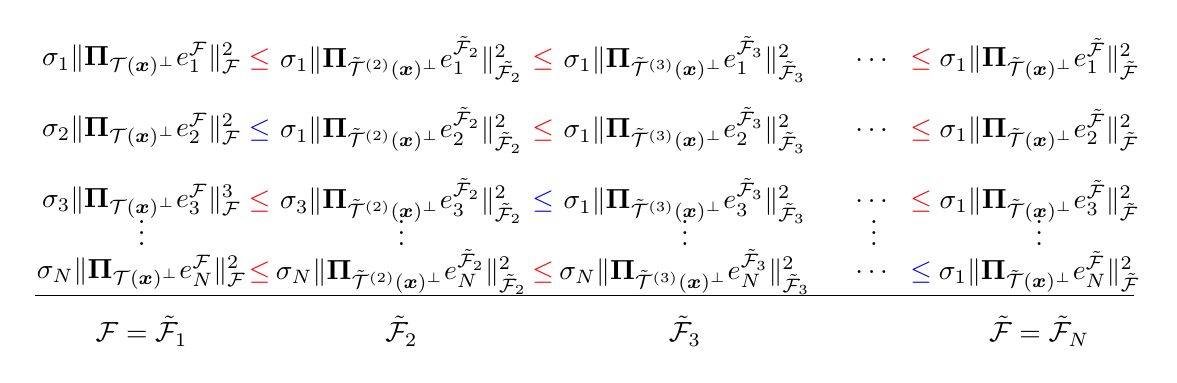
\begin{tikzpicture}[scale = 0.3]

  % draw line and angle
%  \draw 
%     pic [draw,angle radius=4mm,angle eccentricity=1.5, "$\theta$" font=\scriptsize] {angle=v2--v1--v3};

 

%\draw [fill=blue, opacity=0.5] (-15,3.75) -- (-11,3.75) -- (-11,5.5) -- (-15,5.5) -- (-15,3.75);
%\draw [fill=blue, opacity=0.5] (-15,3.5) -- (-11,3.5) -- (-11,3.75) -- (-15,3.75) -- (-15,3.5);
%\draw [fill=blue, opacity=0.5] (-15,3.25) -- (-11,3.25) -- (-11,3.5) -- (-15,3.5) -- (-15,3.25);
%\draw [fill=blue, opacity=0.5] (-15,4) -- (-11,4) -- (-11,3.25) -- (-15,3.25) -- (-15,4);
%\draw [fill=blue, opacity=0.5] (-15,2.75) -- (-11,2.75) -- (-11,4) -- (-15,4) -- (-15,2.75); 
%\draw [fill=blue, opacity=0.5] (-15,2.5) -- (-11,2.5) -- (-11,2.75) -- (-15,2.75) -- (-15,2.5);
%\draw [fill=blue, opacity=0.5] (-15,2.25) -- (-11,2.25) -- (-11,2.5) -- (-15,2.5) -- (-15,2.25);
%\draw [fill=blue, opacity=0.5] (-15,2) -- (-11,2) -- (-11,2.25) -- (-15,2.25) -- (-15,2);
%\draw [fill=blue, opacity=0.5] (-15,1.75) -- (-11,1.75) -- (-11,2) -- (-15,2) -- (-15,1.75);



%\draw [fill=blue, opacity=1] (-2,3.75) -- (2,3.75) -- (2,5.5) -- (-2,5.5) -- (-2,3.75);
%\draw [fill=blue, opacity=1] (-2,3.5) -- (2,3.5) -- (2,3.75) -- (-2,3.75) -- (-2,3.5);
%\draw [fill=blue, opacity=0.5] (-2,3.25) -- (2,3.25) -- (2,3.5) -- (-2,3.5) -- (-2,3.25);
%\draw [fill=blue, opacity=0.5] (-2,4) -- (2,4) -- (2,3.25) -- (-2,3.25) -- (-2,4);
%\draw [fill=blue, opacity=1] (-2,2.75) -- (2,2.75) -- (2,4) -- (-2,4) -- (-2,2.75); 
%\draw [fill=blue, opacity=0.5] (-2,2.5) -- (2,2.5) -- (2,2.75) -- (-2,2.75) -- (-2,2.5);
%\draw [fill=blue, opacity=0.5] (-2,2.25) -- (2,2.25) -- (2,2.5) -- (-2,2.5) -- (-2,2.25);
%\draw [fill=blue, opacity=1] (-2,2) -- (2,2) -- (2,2.25) -- (-2,2.25) -- (-2,2);
%\draw [fill=blue, opacity=0.5] (-2,1.75) -- (2,1.75) -- (2,2) -- (-2,2) -- (-2,1.75);





%\draw [fill=blue, opacity=1] (13,2.75) -- (17,2.75) -- (17,4) -- (13,4) -- (13,2.75);
%\draw [fill=blue, opacity=1] (13,2.5) -- (17,2.5) -- (17,2.75) -- (13,2.75) -- (13,2.5);
%\draw [fill=blue, opacity=1] (13,2.25) -- (17,2.25) -- (17,2.5) -- (13,2.5) -- (13,2.25);
%\draw [fill=blue, opacity=1] (13,2) -- (17,2) -- (17,2.25) -- (13,2.25) -- (13,2);


%\draw [fill=orange, opacity=1] (13.25,2) -- (13.25,2) -- (13.5,2) -- (13.5,4) -- (13.25,4);
%\draw [fill=orange, opacity=1] (14.25,2) -- (14.25,2) -- (14.5,2) -- (14.5,4) -- (14.25,4);
%\draw [fill=orange, opacity=1] (14.75,2) -- (14.75,2) -- (15,2) -- (15,4) -- (14.75,4);
%\draw [fill=orange, opacity=1] (15.75,2) -- (15.75,2) -- (16,2) -- (16,4) -- (15.75,4);



%\draw [->] (-7.5,2) --  (-6.5,2)  node [above] {\tiny $\Prb(T) \propto \prod_{i \in T} \sigma_{i}^{2}$} --  (-5.5,2);

%\draw [->] (6.5,2) --  (7.5,2)  node [above] {\tiny $\Prb(S|T) = \Det (\bm{V}_{S,T})^{2}$} --  (11.5,2);

%\draw  (-17,2.25)  node [above] {$\bm{V}^{\Tran}=$} ;

\draw  (-43,7)  node  {$\sigma_{1}\|\bm{\Pi}_{\mathcal{T}(\bm{x})^{\perp}}e_{1}^{\mathcal{F}}\|^{2}_{\mathcal{F}}$} ;
\draw  (-38,7)  node  {$\color{red} \leq$} ;
\draw  (-32,7)  node  {$\sigma_{1}\|\bm{\Pi}_{\tilde{\mathcal{T}}^{(2)}(\bm{x})^{\perp}}e_{1}^{\tilde{\mathcal{F}}_{2}}\|^{2}_{\tilde{\mathcal{F}_{2}}}$} ;
\draw  (-26,7)  node  {$\color{red} \leq$} ;
\draw  (-20,7)  node  {$\sigma_{1}\|\bm{\Pi}_{\tilde{\mathcal{T}}^{(3)}(\bm{x})^{\perp}}e_{1}^{\tilde{\mathcal{F}}_{3}}\|^{2}_{\tilde{\mathcal{F}}_{3}}$} ;
%\draw  (-20,7)  node  {$\leq$} ;
\draw  (-12,7)  node  {$\dots$} ;

\draw  (-10,7)  node  {$\color{red} \leq$} ;
\draw  (-5,7)  node  {$\sigma_{1}\|\bm{\Pi}_{\tilde{\mathcal{T}}(\bm{x})^{\perp}}e_{1}^{\tilde{\mathcal{F}}}\|^{2}_{\tilde{\mathcal{F}}}$} ;




\draw  (-43,4)  node  {$\sigma_{2}\|\bm{\Pi}_{\mathcal{T}(\bm{x})^{\perp}}e_{2}^{\mathcal{F}}\|^{2}_{\mathcal{F}}$} ;
\draw  (-38,4)  node  {$\color{blue} \leq$} ;
\draw  (-32,4)  node  {$\sigma_{1}\|\bm{\Pi}_{\tilde{\mathcal{T}}^{(2)}(\bm{x})^{\perp}}e_{2}^{\tilde{\mathcal{F}}_{2}}\|^{2}_{\tilde{\mathcal{F}}_{2}}$} ;
\draw  (-26,4)  node  {$\color{red} \leq$} ;
\draw  (-20,4)  node  {$\sigma_{1}\|\bm{\Pi}_{\tilde{\mathcal{T}}^{(3)}(\bm{x})^{\perp}}e_{2}^{\tilde{\mathcal{F}}_{3}}\|^{2}_{\tilde{\mathcal{F}}_{3}}$} ;
%\draw  (-20,7)  node  {$\leq$} ;
\draw  (-12,4)  node  {$\dots$} ;

\draw  (-10,4)  node  {$\color{red} \leq$} ;
\draw  (-5,4)  node  {$\sigma_{1}\|\bm{\Pi}_{\tilde{\mathcal{T}}(\bm{x})^{\perp}}e_{2}^{\tilde{\mathcal{F}}}\|^{2}_{\tilde{\mathcal{F}}}$} ;


\draw  (-43,1)  node  {$\sigma_{3}\|\bm{\Pi}_{\mathcal{T}(\bm{x})^{\perp}}e_{3}^{\mathcal{F}}\|^{3}_{\mathcal{F}}$} ;
\draw  (-38,1)  node  {$\color{red} \leq$} ;
\draw  (-32,1)  node  {$\sigma_{3}\|\bm{\Pi}_{\tilde{\mathcal{T}}^{(2)}(\bm{x})^{\perp}}e_{3}^{\tilde{\mathcal{F}}_{2}}\|^{2}_{\tilde{\mathcal{F}}_{2}}$} ;
\draw  (-26,1)  node  {$\color{blue} \leq$} ;
\draw  (-20,1)  node  {$\sigma_{1}\|\bm{\Pi}_{\tilde{\mathcal{T}}^{(3)}(\bm{x})^{\perp}}e_{3}^{\tilde{\mathcal{F}}_{3}}\|^{2}_{\tilde{\mathcal{F}}_{3}}$} ;
%\draw  (-20,7)  node  {$\leq$} ;
\draw  (-12,1)  node  {$\dots$} ;

\draw  (-10,1)  node  {$\color{red} \leq$} ;
\draw  (-5,1)  node  {$\sigma_{1}\|\bm{\Pi}_{\tilde{\mathcal{T}}(\bm{x})^{\perp}}e_{3}^{\tilde{\mathcal{F}}}\|^{2}_{\tilde{\mathcal{F}}}$} ;


\draw  (-43,0)  node  {$\vdots$} ;
%\draw  (-36,0)  node  {$\leq$} ;
\draw  (-32,0)  node  {$\vdots$} ;
%\draw  (-28,0)  node  {$\leq$} ;
\draw  (-20,0)  node  {$\vdots$} ;
%\draw  (-20,7)  node  {$\leq$} ;
\draw  (-12,0)  node  {$\vdots$} ;

%\draw  (-12,0)  node  {$\leq$} ;
\draw  (-5,0)  node  {$\vdots$} ;



\draw  (-43,-2)  node  {$\sigma_{N}\|\bm{\Pi}_{\mathcal{T}(\bm{x})^{\perp}}e_{N}^{\mathcal{F}}\|^{2}_{\mathcal{F}}$} ;
\draw  (-38,-2)  node  {$\color{red} \leq$} ;
\draw  (-32,-2)  node  {$\sigma_{N}\|\bm{\Pi}_{\tilde{\mathcal{T}}^{(2)}(\bm{x})^{\perp}}e_{N}^{\tilde{\mathcal{F}}_{2}}\|^{2}_{\tilde{\mathcal{F}}_{2}}$} ;
\draw  (-26,-2)  node  {$\color{red} \leq$} ;
\draw  (-20,-2)  node  {$\sigma_{N}\|\bm{\Pi}_{\tilde{\mathcal{T}}^{(3)}(\bm{x})^{\perp}}e_{N}^{\tilde{\mathcal{F}}_{3}}\|^{2}_{\tilde{\mathcal{F}}_{3}}$} ;
%\draw  (-20,7)  node  {$\leq$} ;
\draw  (-12,-2)  node  {$\dots$} ;

\draw  (-10,-2)  node  {$\color{blue} \leq$} ;
\draw  (-5,-2)  node  {$\sigma_{1}\|\bm{\Pi}_{\tilde{\mathcal{T}}(\bm{x})^{\perp}}e_{N}^{\tilde{\mathcal{F}}}\|^{2}_{\tilde{\mathcal{F}}}$} ;

\draw[line width=0.15 mm] (-47.5,-3) -- (-1,-3);

\draw  (-43,-4.5)  node  {$\mathcal{F}=\tilde{\mathcal{F}}_{1}$} ;
\draw  (-38,-4.5)  node  {} ;
\draw  (-32,-4.5)  node  {$\tilde{\mathcal{F}}_{2}$} ;
\draw  (-26,-4.5)  node  {} ;
\draw  (-20,-4.5)  node  {$\tilde{\mathcal{F}}_{3}$} ;
%\draw  (-20,7)  node  {$\leq$} ;
\draw  (-12,-4.5)  node  {} ;

\draw  (-10,-4.5)  node  {} ;
\draw  (-5,-4.5)  node  {$\tilde{\mathcal{F}} = \tilde{\mathcal{F}}_{N}$} ;
\end{tikzpicture}

% \pc{Peut-être introduire $\Delta_n^{\cal F}(\bm{x}) = e_{n}^{\mathcal{F}}(\bm{x})^{\Tran}\bm{K}(\bm{x})^{-1}e_{n}^{\mathcal{F}}(\bm{x})$ et  $\Delta_n^{\tilde{\cal F}_\ell}(\bm{x}) = e_{n}^{\tilde{\mathcal{F}}_{\ell}}(\bm{x})^{\Tran}\tilde{\bm{K}}^{(\ell)}(\bm{x})^{-1}e_{n}^{\tilde{\mathcal{F}}_{\ell}}(\bm{x})$ pour alléger l'écriture avec $\l...\l$ partout ?}
% %\subfloat[]{\includegraphics{img/BernoulliKernels/Bernoulli_kernels_same_node_s_1_5_zoom.pdf}} \\
% \caption{The illustration of the inequalities in Proposition~\ref{prop:graded_RKHS}. The inequality \eqref{eq:graded_RKHS_inequality_1} is in blue and the inequality \eqref{eq:graded_RKHS_inequality_2} is in red. \label{fig:graded_RKHS}}
% \end{figure}



%%%%%%%% Proposition 3 : a) Proposition 2, b) Lemma 2, c) Lemma 4, d) Lemma 5

\subsubsection{Proof of Proposition~\ref{prop:expected_value_of_product_of_cos}}
\label{s:proofOfExpectedProduct}
% Remark
%\subsection{A bound for $\displaystyle \EX_{\DPP} \prod\limits_{\ell \in [N]} \frac{1}{\cos^{2} \theta_{\ell}\left(\mathcal{E}^{\mathcal{F}}_{N}, \mathcal{T}(x) \right)}$}
%\pc{Revoir titre : j'ai enlevé le titre "A bound for $\displaystyle \EX_{\DPP} \prod\limits_{\ell \in [N]} \frac{1}{\cos^{2} \theta_{\ell}\left(\mathcal{E}^{\mathcal{F}}_{N}, \mathcal{T}(x) \right)}$"}
%

In this section, $\bm{x}  = (x_{1}, \dots , x_{N}) \in \mathcal{X}^{N}$ is the realization of the DPP of Theorem~\ref{thm:main_theorem}. Let $\bm{E}^{\mathcal{F}}(\bm{x}) = (e_{i}^{\mathcal{F}}(x_{j}))_{1 \leq i,j \leq N}$ and $\bm{E}(\bm{x}) = (e_{i}(x_{j}))_{1 \leq i,j \leq N}$, and $\bm{K}(\bm{x})= (k(x_{i},x_{j}))_{1 \leq i,j \leq N} $.
Moreover, let $\mathcal{E}^{\mathcal{F}}_{N} = \Span(e_{m}^{\mathcal{F}})_{m \in [N]}$ and $\mathcal{T}(\bm{x}) =  \Span \left( k(x_{i},.) \right)_{i \in [N]}$.

We first prove two lemmas that are necessary to prove Proposition~\ref{prop:expected_value_of_product_of_cos}.

%%%
\paragraph{Two preliminary lemmas}

%%% Lemma 4
%%%%%%
\begin{lemma}\label{lemma:cos_ratio_det}
Let $\bm{x} =  (x_{1}, \dots , x_{N}) \in \mathcal{X}^{N} $ such that $\Det^{2} \bm{E}(\bm{x}) \neq 0$. Then,
\begin{equation}
\prod\limits_{\ell \in [N]} \frac{1}{\cos^{2} \theta_{\ell} \left(\mathcal{E}^{\mathcal{F}}_{N}, \mathcal{T}(\bm{x}) \right)} = \frac{\Det \bm{K}(\bm{x})}{\Det^{2} \bm{E}^{\mathcal{F}}(\bm{x})}.
\end{equation}
\end{lemma}

\begin{proof}
The condition $\Det^{2} \bm{E}(\bm{x}) \neq 0$ yields by Proposition~\ref{prop:K_N_non_singular} that $\bm{K}(\bm{x})$ is non singular. Thus $\dim \mathcal{T}(\bm{x}) = N$. Let $(t_{i})_{i \in [N]}$ an orthonormal basis of $\mathcal{T}(\bm{x})$ with respect to $\langle ., . \rangle_{\mathcal{F}}$.
%
Using Corollary~\ref{cor:cos_det_relationship}, and the fact that $(e_{n}^{\mathcal{F}})_{n \in [N]}$ is an orthonormal basis of $\mathcal{E}^{\mathcal{F}}_{N}$ according to $\langle ., . \rangle_{\mathcal{F}}$,
\begin{equation}\label{eq:prod_cos_det_E}
\prod\limits_{\ell \in [N]} \cos^{2} \theta_{\ell} \left(\mathcal{E}^{\mathcal{F}}_{N}, \mathcal{T}(\bm{x}) \right) = \Det^{2} (\langle e_{n}^{\mathcal{F}}, t_{i} \rangle_{\mathcal{F}})_{(n,i) \in [N]\times[N]}.
\end{equation}
Now, write for $i \in [N]$,
\begin{equation}\label{eq:t_as_function_of_kx}
t_{i} = \sum\limits_{j \in [N]} c_{i,j} k(x_{j},.).
\end{equation}
%
Thus
\begin{align}
\langle e_{n}^{\mathcal{F}}, t_{i} \rangle_{\mathcal{F}} = & \sum\limits_{j \in [N]} c_{i,j} \langle e_{n}^{\mathcal{F}}, k(x_{j},.) \rangle_{\mathcal{F}} \\
= &\sum\limits_{j \in [N]} c_{i,j}  e_{n}^{\mathcal{F}}(x_{j}).
\end{align}
%
Then
\begin{equation}
(\langle e_{n}^{\mathcal{F}}, t_{i} \rangle_{\mathcal{F}})_{(n,i) \in [N]\times[N]} = \bm{E}^{\mathcal{F}}(\bm{x}) \bm{C}(\bm{x})^{\Tran} ,
\end{equation}
where
\begin{equation}
\bm{C}(\bm{x}) = (c_{i,j})_{1 \leq i,j \leq N}.
\end{equation}
%
Thus
\begin{equation}\label{eq:AN_times_EN}
\Det^{2} (\langle e_{n}^{\mathcal{F}}, t_{i} \rangle_{\mathcal{F}})_{(n,i) \in [N]\times[N]} = \Det^{2} \bm{C}(\bm{x}) \Det^{2} \bm{E}^{\mathcal{F}}(\bm{x}).
\end{equation}
%%%%
Now, let $\bm{c}_{i}$ the columns of the matrix $\bm{C}(\bm{x})$. $(t_{i})_{i \in [N]}$ is an orthonormal basis of $\mathcal{T}(\bm{x})$ with respect to $\langle .,. \rangle_{\mathcal{F}}$, then by \eqref{eq:t_as_function_of_kx}
\begin{equation}
  \delta_{i,i'} = \langle t_{i}, t_{i'} \rangle_{\mathcal{F}} = \bm{c}_{i}^{\Tran} \bm{K}(\bm{x}) \bm{c}_{i'}  .
\end{equation}
Therefore
\begin{equation}
\bm{C}(\bm{x})^{\Tran} \bm{K}(\bm{x}) \bm{C}(\bm{x}) = \mathbb{I}_{N}.
\end{equation}
Thus
\begin{equation}\label{eq:det_AN_det_KN_relationship}
\Det^{2} \bm{C}(\bm{x}) = \frac{1}{\Det \bm{K}(\bm{x})}.
\end{equation}
Combining \eqref{eq:prod_cos_det_E}, \eqref{eq:AN_times_EN} and \eqref{eq:det_AN_det_KN_relationship} concludes the proof of Lemma~\ref{lemma:cos_ratio_det}:
\begin{equation}
\prod\limits_{\ell \in [N]} \frac{1}{\cos^{2} \theta_{\ell} \left(\mathcal{E}^{\mathcal{F}}_{N}, \mathcal{T}(\bm{x}) \right)} = \frac{\Det \bm{K}(\bm{x})}{\Det^{2} \bm{E}^{\mathcal{F}}(\bm{x})}.
\end{equation}
\end{proof}



%%%%%% Lemma 5
\begin{lemma}\label{lemma:truncated_Fredholm_formula}
\begin{equation}
  \frac{1}{N!} \int_{\mathcal{X}^{N}}\Det \bm{K}(x_{1}, \dots, x_{N}) \otimes_{j \in [N]} \mathrm{d}\omega(x_{j})  = \sum\limits_{\substack{T \subset \mathbb{N}^{*} \\ |T| = N}}  \prod\limits_{t \in T}\sigma_{t}.
\end{equation}
\end{lemma}
%% Proof
\begin{proof}
Let $\bm{x} = (x_{1}, \dots, x_{N}) \in \mathcal{X}^{N}$. From \eqref{eq:truncated_kernel_limit}
\begin{equation}
\Det \bm{K}(\bm{x}) = \lim\limits_{M \rightarrow \infty} \Det \bm{K}_{M}(\bm{x}).
\end{equation}
Moreover,
\begin{equation}
\Det \bm{K}_{M}(\bm{x})  = \sum\limits_{T \subset [M], |T| = N} \prod\limits_{i \in T} \sigma_{i} \Det^{2} (e_{i}(x_{j}))_{(i,j)\in T \times [N]}.
\end{equation}
Now, for $T \subset [M]$ such that $|T| = N$, $(e_{t})_{t \in T}$ is an orthonormal family of $\mathbb{L}_{2}(\mathrm{d}\omega)$, then by \cite{HoKrPeVi06} Lemma 21:
\begin{equation}
\int_{\mathcal{X}^{N}}\Det^{2} (e_{t}(x_{j})) \otimes_{j \in [N]} \mathrm{d}\omega(x_{j}) = N! .
\end{equation}

Thus
\begin{align}
\frac{1}{N!} \int_{\mathcal{X}^{N}}\Det \bm{K}_{M}(\bm{x}) \otimes_{j \in [N]} \mathrm{d}\omega(x_{j}) &=  \frac{1}{N!} \sum\limits_{T \subset [M], |T| = N} \prod\limits_{t \in T} \sigma_{t} \int_{\mathcal{X}^{N}}\Det^{2} (e_{t}(x_{j})) \otimes_{j \in [N]} \mathrm{d}\omega(x_{j}) \\
& = \sum\limits_{T \subset [M], |T| = N} \prod\limits_{t \in T} \sigma_{t} \nonumber.
\end{align}
Now, $\displaystyle \sum\limits_{n \in \mathbb{N}^{*}} \sigma_{n} < \infty$ implies that $\displaystyle \sum\limits_{T \subset \mathbb{N}^{*}, |T| = N} \prod\limits_{t \in T} \sigma_{t} < \infty$. In fact, for $\ell \in [N]$ let $p_{\ell}$ the $\ell$-th symmetric polynomial. By Maclaurin’s inequality \citep{Ste04}, and for any vector $\bm{\nu} \in \mathbb{R}_{+}^{M}$
\begin{equation}
\left( \frac{p_{\ell}(\bm{\nu})}{{M\choose \ell}} \right)^{\frac{1}{\ell}} \leq \frac{p_{1}(\bm{\nu})}{M}.
\end{equation}
Thus
\begin{align}\label{eq:Maclaurin_inequality}
p_{\ell}(\bm{\nu}) & \leq  \frac{{M\choose \ell}}{M^{\ell}}p_{1}(\bm{\nu})^{\ell} \\
& \leq \frac{M!}{\ell!(M-\ell)! M^{\ell}}p_{1}(\bm{\nu})^{\ell} \nonumber\\
& \leq \frac{M (M-1) \dots (M-\ell +1)}{\ell! M^{\ell}}p_{1}(\bm{\nu})^{\ell} \nonumber\\
& \leq \frac{1}{\ell !}p_{1}(\bm{\nu})^{\ell} \nonumber.
\end{align}
This inequality is independent of the dimension $M$ thus it can be extended for $\bm{\nu} \in \mathbb{R}_{+}^{\mathbb{N}^{*}}$ with $\displaystyle \sum\limits_{n \in \mathbb{N}^{*}} \nu_{n} < \infty$. Therefore
\begin{equation}
\sum\limits_{T \subset \mathbb{N}^{*}, |T| = N} \prod\limits_{t \in T} \sigma_{t}  \leq \frac{1}{N!} (\sum\limits_{n \in \mathbb{N}^{*}} \sigma_{n})^{N} < \infty .
\end{equation}

Furthermore,
\begin{equation}
\forall M \in \mathbb{N}^{*}, \: \forall \bm{x} \in \mathcal{X}^{N}, \: 0 \leq \Det \bm{K}_{M}(\bm{x}) \leq \Det \bm{K}_{M+1,N}(\bm{x}).
\end{equation}
Then by monotone convergence theorem, $\displaystyle \bm{x} \mapsto \frac{1}{N!}\Det \bm{K}(\bm{x})$ is mesurable and
\begin{align}
\int_{\mathcal{X}^{N}} \frac{1}{N!}\Det \bm{K}(\bm{x}) \otimes_{j \in [N]} \mathrm{d}\omega(x_j) & = \lim\limits_{M \rightarrow \infty} \int_{\mathcal{X}^{N}}\frac{1}{N!} \Det \bm{K}_{M}(\bm{x})\otimes_{j \in [N]} \mathrm{d}\omega(x_j)\\
& = \lim\limits_{M \rightarrow \infty} \sum\limits_{T \subset [M], |T| = N} \prod\limits_{t \in T} \sigma_{t} \nonumber\\
& = \sum\limits_{T \subset \mathbb{N}^{*}, |T| = N} \prod\limits_{t \in T} \sigma_{t} \nonumber.
\end{align}
% thanks to the convergence of $\displaystyle \sum\limits_{n \in \mathbb{N}} \sigma_{n} < \infty$.
\end{proof}

%%%%%%%%%%%%%%%% Proposition 3
\paragraph{End of the proof of Proposition~\ref{prop:expected_value_of_product_of_cos}}
%Now we can prove Proposition~\ref{prop:expected_value_of_product_of_cos} thanks to Lemmas~\ref{lemma:cos_ratio_det} \& \ref{lemma:truncated_Fredholm_formula} above.
\begin{proof}
Remember that
\begin{equation}
\Prb \left( \Det \bm{E}(\bm{x})  \neq 0 \right) = 1.
\end{equation}
Then by Lemma~\ref{lemma:cos_ratio_det} and the fact that $\Det^{2} \bm{E}^{\mathcal{F}}(\bm{x}) = \prod\limits_{n \in [N]} \sigma_{n} \Det^{2} \bm{E}(\bm{x})$
\begin{equation}
\prod\limits_{\ell \in [N]} \frac{1}{\cos^{2} \theta_{\ell} \left(\mathcal{E}^{\mathcal{F}}_{N}, \mathcal{T}(\bm{x}) \right)} = \frac{\Det \bm{K}(\bm{x})}{\Det^{2} \bm{E}^{\mathcal{F}}(\bm{x})} = \frac{1}{\prod\limits_{n \in [N]} \sigma_{n}}\frac{\Det \bm{K}(\bm{x})}{\Det^{2} \bm{E}(\bm{x})}.
\end{equation}
Then, taking the expectation with respect to $\bm{x}$ resulting from a DPP of kernel $\KDPP(x,y)$,
\begin{align}
\EX_{\DPP} \prod\limits_{\ell \in [N]} \frac{1}{\cos^{2} \theta_{\ell}\left(\mathcal{E}^{\mathcal{F}}_{N}, \mathcal{T}(\bm{x}) \right)} = & \frac{1}{N!} \int_{\mathcal{X}^{N}} \Det^{2} \bm{E}(\bm{x}) \prod\limits_{\ell \in [N]} \frac{1}{\cos^{2} \theta_{\ell} \left(\mathcal{E}^{\mathcal{F}}_{N}, \mathcal{T}(\bm{x}) \right)} \otimes_{i =1}^{N} \mathrm{d}\omega(x_{i}) \\
 = & \frac{1}{N!} \int_{\mathcal{X}^{N}} \Det^{2} \bm{E}(\bm{x}) \frac{1}{\prod\limits_{n \in [N]} \sigma_{n}}\frac{\Det \bm{K}(\bm{x})}{\Det^{2} \bm{E}(\bm{x})} \otimes_{i =1}^{N} \mathrm{d}\omega(x_{i}) \nonumber\\
 = & \frac{1}{\prod\limits_{n \in [N]} \sigma_{n}} \frac{1}{N!} \int_{\mathcal{X}^{N}}\Det \bm{K}(\bm{x}) \otimes_{i =1}^{N} \mathrm{d}\omega(x_{i}) \nonumber.
\end{align}
Now, by Lemma~\ref{lemma:truncated_Fredholm_formula}
\begin{equation}
\frac{1}{N!} \int_{\mathcal{X}^{N}}\Det \bm{K}(\bm{x}) \otimes_{i =1}^{N} \mathrm{d}\omega(x_{i})  = \sum\limits_{\substack{T \subset \mathbb{N}^{*} \\ |T| = N}}  \prod\limits_{t \in T}\sigma_{t}.
\end{equation}
Therefore,
\begin{equation}
\EX_{\DPP} \prod\limits_{\ell \in [N]} \frac{1}{\cos^{2} \theta_{\ell}\left(\mathcal{E}^{\mathcal{F}}_{N}, \mathcal{T}(\bm{x}) \right)}  =  \sum\limits_{\substack{T \subset \mathbb{N}^{*} \\ |T| = N}} \frac{ \prod\limits_{t \in T}\sigma_{t}}{\prod\limits_{n \in [N]} \sigma_{n}}.
\end{equation}

\end{proof}


%%%%%%%% Theorem 1
%%%%%%%%%%%%%%%%%% Main Theorem
\subsubsection{Proof of Theorem~\ref{thm:main_theorem}}
\label{s:finalBound}
\begin{proof}
Thanks to Proposition~\ref{prop:kernel_perturbation_inequality} and Lemma~\ref{lemma:max_error_cos} (for $\tilde{\cal F}$ and $\tilde{k}$)
\begin{align}\label{eq:prooftheorem1_first}
  \max_{ n \in [N]}\sigma_n \|\bm{\Pi}_{\mathcal{T}(\bm{x})^{\perp}} e_{n}^{\mathcal{F}}\|_{\mathcal{F}}^{2}
  & \leq
  \sigma_1 \cdot \max_{ n \in [N]} \|\bm{\Pi}_{\tilde{\cal{T}}(\bm{x})^{\perp}} e_{n}^{\tilde{\mathcal{F}}}\|_{\tilde{\mathcal{F}}}^{2}\\
  & \leq
  \sigma_1 \cdot \left( \prod\limits_{n \in [N]}\frac{1}{\cos^{2} \theta_{n}(\tilde{\cal{T}}(\bm{x}),\mathcal{E}^{\tilde{\mathcal{F}}}_{N})} - 1\right).
\end{align}
%
%\begin{equation}
% \EX_{\DPP} \prod\limits_{\ell \in [N]} \frac{1}{\cos^{2} \theta_{\ell}\left(\mathcal{E}^{\tilde{\mathcal{F}}}_{N}, \tilde{\mathcal{T}}_{N}(\bm{x}) \right)}  \leq \EX_{\DPP} \prod\limits_{\ell \in [N]} \frac{1}{\cos^{2} \theta_{\ell}\left(\mathcal{E}^{\tilde{\mathcal{F}}}_{N}, \tilde{\mathcal{T}}_{N}(\bm{x}) \right)}
%\end{equation}
%
Then Proposition~\ref{prop:expected_value_of_product_of_cos} applied to $\tilde{\cal F}$ with kernel $\tilde{k}$ yields
\begin{equation}
  \EX_{\DPP} \prod\limits_{n \in [N]} \frac{1}{\cos^{2} \theta_{n}\left(\mathcal{E}^{\tilde{\mathcal{F}}}_{N}, \tilde{\mathcal{T}}_{N}(\bm{x}) \right)}   =
  \sum\limits_{\substack{T \subset \mathbb{N}^{*} \\ |T| = N}} \frac{ \prod\limits_{t \in T}\tilde{\sigma}_{t}}{\prod\limits_{n \in [N]} \tilde{\sigma}_{n}}.
\end{equation}
%
Every subset $T \subset \mathbb{N}^{*}$ such that $|T| = N$ can be written as $T = V \cup W$ with $V \subset [N]$ and $W \subset \mathbb{N}^{*} \smallsetminus [N]$, and this decomposition is unique. Then
\begin{equation}
\frac{ \prod\limits_{t \in T}\tilde{\sigma}_{t}}{\prod\limits_{n \in [N]} \tilde{\sigma}_{n}} = \frac{\prod\limits_{v \in V}\tilde{\sigma}_{v} \prod\limits_{w \in W}\tilde{\sigma}_{w}}{\prod\limits_{n \in [N]} \tilde{\sigma}_{n}} = \frac{\prod\limits_{w \in W}\tilde{\sigma}_{w}}{\prod\limits_{n \in [N]\smallsetminus V} \tilde{\sigma}_{n}}.
\end{equation}
Therefore
\begin{align}
  \sum\limits_{\substack{T \subset \mathbb{N}^{*} \\ |T| = N}} \frac{ \prod\limits_{t \in T}\tilde{\sigma}_{t}}{\prod\limits_{n \in [N]} \tilde{\sigma}_{n}} & = \sum\limits_{\substack{T \subset \mathbb{N}^{*} \\ |T| = N\\ T = V \cup W}} \frac{\prod\limits_{w \in W}\tilde{\sigma}_{w}}{\prod\limits_{n \in [N]\smallsetminus V} \tilde{\sigma}_{n}} \\
  & = \sum\limits_{V \subset [N]}\sum\limits_{\substack{W \subset \mathbb{N}^{*}\smallsetminus [N]\\ |W| = N-|V|}} \frac{\prod\limits_{w \in W}\tilde{\sigma}_{w}}{\prod\limits_{n \in [N]\smallsetminus V} \tilde{\sigma}_{n}} \nonumber\\
  & = \sum\limits_{0 \leq \ell \leq N} \bigg[ \sum\limits_{\substack{V \subset [N]\\ |V| = \ell}}\prod\limits_{n \in [N]\smallsetminus V} \frac{1}{\tilde{\sigma}_{n}}\bigg]\bigg[\sum\limits_{\substack{W \subset \mathbb{N}^{*}\smallsetminus [N]\\ |W| = N-\ell}} \prod\limits_{w \in W}\tilde{\sigma}_{w}\bigg] \nonumber\\
  & = \sum\limits_{0 \leq \ell \leq N} \bigg[\sum\limits_{\substack{V \subset [N]\\ |V| = N-\ell}}\prod\limits_{n \in V} \frac{1}{\tilde{\sigma}_{n}}\bigg] \bigg[\sum\limits_{\substack{W \subset \mathbb{N}^{*}\smallsetminus [N]\\ |W| = N-\ell}} \prod\limits_{w \in W}\tilde{\sigma}_{w}\bigg] \nonumber\\
  & = \sum\limits_{0 \leq \ell \leq N} p_{N-\ell}\left(\left(\frac{1}{\tilde{\sigma}_{m}}\right)_{m \in [N]}\right)p_{N-\ell}\left((\tilde{\sigma}_{m})_{m \geq N+1}\right) \nonumber\\
  & = \sum\limits_{0 \leq \ell \leq N} p_{\ell}\left(\left(\frac{1}{\tilde{\sigma}_{m}}\right)_{m \in [N]}\right)p_{\ell}\left((\tilde{\sigma}_{m})_{m \geq N+1}\right) \nonumber,
\end{align}
where for $\ell \in [N]$, $p_{\ell}$ is the $\ell$-th symmetric polynomial with the convention that $p_{0} = 1$.

%
Finally, thanks to \eqref{eq:Maclaurin_inequality} above
\begin{align}
  \sum\limits_{\substack{T \subset \mathbb{N}^{*} \\ |T| = N}} \frac{ \prod\limits_{t \in T}\tilde{\sigma}_{t}}{\prod\limits_{n \in [N]} \tilde{\sigma}_{n}}
  & \leq  1 + \sum\limits_{\ell \in [N]} \frac{1}{\ell!^{2}} \left(\sum\limits_{m \in [N]}\frac{1}{\tilde{\sigma}_{m}} \sum\limits_{m \geq N+1} \tilde{\sigma}_{m}\right)^{\ell} \\
  & \leq 1+ \sum\limits_{\ell \in [N]} \frac{1}{\ell!^{2}} \left(\frac{N}{\sigma_1} \sum\limits_{m \geq N+1} \sigma_{m}\right)^{\ell} \nonumber.
\end{align}
%
As a consequence, by writing $r_{N} = \sum\limits_{m \geq N+1} \sigma_{m}$,
\begin{equation}
  \EX_{\DPP} \left[ \max_{ n \in [N]}\sigma_n \|\bm{\Pi}_{\mathcal{T}(\bm{x})^{\perp}} e_{n}^{\mathcal{F}}\|_{\mathcal{F}}^{2} \right]
  \leq
  \sigma_1 \cdot \sum_{\ell=1}^{N} \frac{1}{\ell!^{2}} \left(\frac{N  r_{N} }{\sigma_1}\right)^{\ell}
% \sigma_1 \cdot \sum_{\ell=1}^{N} \frac{1}{\ell!^{2}} \left(\frac{N}{\sigma_1} \sum\limits_{m \geq N+1} \sigma_{m}\right)^{\ell}
\end{equation}
which can be plugged in Lemma~\ref{lemma:approximation_error_spectral_bound} to conclude the proof.
\end{proof}


\subsubsection{The proofs of the strong version}
Our objective in this section is to give a tractable expression of 
\begin{equation}
\EX_{\DPP} \sum\limits_{\ell \in [N]} \frac{1}{\cos^{2} \theta_{\ell} \bigg(\mathcal{E}^{\mathcal{F}}_{N}, \mathcal{T}(\bm{x}) \bigg)}.
\end{equation}
We start by proving the following result.
%%%%%%
\begin{lemma}\label{lemma:sum_inverse_cos}
Let $\bm{x} =  (x_{1}, \dots , x_{N}) \in \mathcal{X}^{N} $ such that $\Det^{2} \bm{E}(\bm{x}) \neq 0$. Then,
\begin{equation}
\sum\limits_{\ell \in [N]} \frac{1}{\cos^{2} \theta_{\ell} \bigg(\mathcal{E}^{\mathcal{F}}_{N}, \mathcal{T}(\bm{x}) \bigg)} = \Tr \bigg(\bm{E}^{\mathcal{F}}(\bm{x})^{\Tran^{-1}}  \bm{K}(\bm{x}) \bm{E}^{\mathcal{F}}(\bm{x})^{-1} \bigg).
\end{equation}
\end{lemma}

\begin{proof}
We proceed as in the proof of Lemma~\ref{lemma:cos_ratio_det}. 
The condition $\Det^{2} \bm{E}(\bm{x}) \neq 0$ yields by Proposition~\ref{prop:K_N_non_singular} that $\bm{K}(\bm{x})$ is non singular. Thus $\dim \mathcal{T}(\bm{x}) = N$. Let $(t_{i})_{i \in [N]}$ be an orthonormal basis of $\mathcal{T}(\bm{x})$ with respect to $\langle ., . \rangle_{\mathcal{F}}$ and let $\bm{W}(\bm{x}) = \langle e_{n}^{\mathcal{F}}, t_{i} \rangle_{\mathcal{F}}$.
%
Using Corollary~\ref{cor:cos_det_relationship}, and the fact that $(e_{n}^{\mathcal{F}})_{n \in [N]}$ is an orthonormal basis of $\mathcal{E}^{\mathcal{F}}_{N}$ with respect to $\langle ., . \rangle_{\mathcal{F}}$, the $\cos^{2} \theta_{\ell} \bigg(\mathcal{E}^{\mathcal{F}}_{N}, \mathcal{T}(\bm{x}) \bigg)$ are the eigenvalues of the matrix $\bm{W}(\bm{x})\bm{W}(\bm{x})^{\Tran}$. Thus
\begin{equation}\label{eq:sum_cos_tr_E}
\sum\limits_{\ell \in [N]} \frac{1}{\cos^{2} \theta_{\ell} \bigg(\mathcal{E}^{\mathcal{F}}_{N}, \mathcal{T}(\bm{x}) \bigg)} = \Tr \bigg( \bm{W}(\bm{x})\bm{W}(\bm{x})^{\Tran} \bigg)^{-1}.
\end{equation}
Now, using the same analysis as in the proof of Lemma~\ref{lemma:cos_ratio_det}, we get 


% Now, write for $i \in [N]$,
% \begin{equation}\label{eq:t_as_function_of_kx}
% t_{i} = \sum\limits_{j \in [N]} c_{j,i} k(x_{j},.).
% \end{equation}
% %
% Thus
% \begin{align}
% \langle e_{n}^{\mathcal{F}}, t_{i} \rangle_{\mathcal{F}} = & \sum\limits_{j \in [N]} c_{j,i} \langle e_{n}^{\mathcal{F}}, k(x_{j},.) \rangle_{\mathcal{F}} \\
% = &\sum\limits_{j \in [N]}e_{n}^{\mathcal{F}}(x_{j}) c_{j,i}.
% \end{align}
% %
% Then
\begin{equation}
\bm{W}(\bm{x}) = \bm{E}^{\mathcal{F}}(\bm{x})\bm{C}(\bm{x}) ,
\end{equation}
where
\begin{equation}
\bm{C}(\bm{x}) = (c_{j,i})_{1 \leq i,j \leq N}.
\end{equation}
%
Thus
\begin{equation}\label{eq:AN_times_EN}
\bigg( \bm{W}(\bm{x})\bm{W}(\bm{x})^{\Tran} \bigg)^{-1} = \bm{E}^{\mathcal{F}}(\bm{x})^{\Tran^{-1}} \bigg( \bm{C}(\bm{x})\bm{C}(\bm{x})^{\Tran} \bigg)^{-1}  \bm{E}^{\mathcal{F}}(\bm{x})^{-1}
\end{equation}
%%%%
Now, let $\bm{c}_{i}$ the columns of the matrix $\bm{C}(\bm{x})$. $(t_{i})_{i \in [N]}$ is an orthonormal basis of $\mathcal{T}(\bm{x})$ with respect to $\langle .,. \rangle_{\mathcal{F}}$, then by \eqref{eq:t_as_function_of_kx}
\begin{equation}
  \delta_{i,i'} = \langle t_{i}, t_{i'} \rangle_{\mathcal{F}} = \bm{c}_{i}^{\Tran} \bm{K}(\bm{x}) \bm{c}_{i'}  .
\end{equation}
Therefore
\begin{equation}
\bm{C}(\bm{x})^{\Tran} \bm{K}(\bm{x}) \bm{C}(\bm{x}) = \mathbb{I}_{N}.
\end{equation}
Thus
\begin{equation}\label{eq:det_AN_det_KN_relationship}
\bm{K}(\bm{x}) = \bigg( \bm{C}(\bm{x})\bm{C}(\bm{x})^{\Tran} \bigg)^{-1}.
\end{equation}
Combining \eqref{eq:sum_cos_tr_E}, \eqref{eq:AN_times_EN} and \eqref{eq:det_AN_det_KN_relationship} concludes the proof of Lemma~\ref{lemma:sum_inverse_cos}:
\begin{equation}
\sum\limits_{\ell \in [N]} \frac{1}{\cos^{2} \theta_{\ell} \bigg(\mathcal{E}^{\mathcal{F}}_{N}, \mathcal{T}(\bm{x}) \bigg)} = \Tr \bigg(\bm{E}^{\mathcal{F}}(\bm{x})^{\Tran^{-1}} \bm{K}(\bm{x})  \bm{E}^{\mathcal{F}}(\bm{x})^{-1} \bigg).
\end{equation}
\end{proof}
Now, we are ready to prove the main result of this section.
\begin{theorem}
We have
\begin{equation}
\EX_{\DPP}  \sum\limits_{\ell \in [N]} \frac{1}{\cos^{2} \theta_{\ell} \bigg(\mathcal{E}^{\mathcal{F}}_{N}, \mathcal{T}(\bm{x}) \bigg)}  = N + \sum\limits_{v \in [N]} \frac{1}{\sigma_{v}} \sum\limits_{w \in \mathbb{N}^{*}\smallsetminus [N]} \sigma_{w}.
\end{equation}
In particular for the saturated kernel, we have
\begin{equation}
\EX_{\DPP}  \sum\limits_{\ell \in [N]} \frac{1}{\cos^{2} \theta_{\ell} \bigg(\mathcal{E}^{\tilde{\mathcal{F}}}_{N}, \tilde{\mathcal{T}}(\bm{x}) \bigg)}   = N + \frac{N}{\sigma_{1}} \sum\limits_{w \in \mathbb{N}^{*}\smallsetminus [N]} \sigma_{w}.
\end{equation}
\end{theorem}
% We use the following result proved in []
% \begin{lemma} \label{lemma:det_tr_delta_0}
% Let $\bm{A}, \bm{B} \in \mathbb{R}^{N \times N}$ two matrices with the same dimension. Assume that $\Det~\bm{A}~\neq~0$, then
% \begin{equation}
% \partial_{t} \Det (\bm{A}+t\bm{B})_{|t = 0} = \Det(\bm{A}) \Tr(\bm{A}^{-1}\bm{B}).  
% \end{equation} 
% \end{lemma}
\begin{proof}
% \Tr \bigg(  \bm{E}^{\mathcal{F}}(\bm{x})^{\Tran^{-1}}\bm{K}(\bm{x})\bm{E}^{\mathcal{F}}(\bm{x})^{-1} \bigg)
Define $I_{k,N}$ by
\begin{equation}
I_{k,N} = \EX_{\DPP} \sum\limits_{\ell \in [N]} \frac{1}{\cos^{2} \theta_{\ell} \bigg(\mathcal{E}^{\mathcal{F}}_{N}, \mathcal{T}(\bm{x}) \bigg)}.
\end{equation}
By Lemma~\ref{lemma:sum_inverse_cos}, we have
\begin{equation}
\sum\limits_{\ell \in [N]} \frac{1}{\cos^{2} \theta_{\ell} \bigg(\mathcal{E}^{\mathcal{F}}_{N}, \mathcal{T}(\bm{x}) \bigg)} = \Tr \bigg(  \bm{E}^{\mathcal{F}}(\bm{x})^{\Tran^{-1}}\bm{K}(\bm{x})\bm{E}^{\mathcal{F}}(\bm{x})^{-1} \bigg).
\end{equation}
Therefore,
\begin{align}\label{eq:I_k_N}
 I_{k,N} & = \frac{1}{N!} \int_{\mathcal{X}^{N}} \Det^{2}\bm{E}(\bm{x}) \Tr \bigg( \bm{E}^{\mathcal{F}}(\bm{x})^{\Tran^{-1}} \bm{K}(\bm{x}) \bm{E}^{\mathcal{F}}(\bm{x})^{-1}\bigg) \otimes_{j \in [N]} \mathrm{d}\omega(x_{j}) \nonumber\\
& = \frac{1}{N!} \int_{\mathcal{X}^{N}} \Det^{2}\bm{E}(\bm{x}) \Tr \bigg(\bm{E}^{\mathcal{F}}(\bm{x})^{-1} \bm{E}^{\mathcal{F}}(\bm{x})^{\Tran^{-1}} \bm{K}(\bm{x}) \bigg) \otimes_{j \in [N]} \mathrm{d}\omega(x_{j}) \nonumber\\
& = \frac{1}{N!} \int_{\mathcal{X}^{N}} \Det^{2}\bm{E}(\bm{x}) \Tr \bigg(\big(\bm{E}^{\mathcal{F}}(\bm{x})^{\Tran}\bm{E}^{\mathcal{F}}(\bm{x})\big)^{-1}  \bm{K}(\bm{x}) \bigg) \otimes_{j \in [N]} \mathrm{d}\omega(x_{j}) \nonumber\\
& = \frac{1}{N!\prod\limits_{n \in [N]}\sigma_{n}} \int_{\mathcal{X}^{N}} \Det^{2}\bm{E}^{\mathcal{F}}(\bm{x}) \Tr \bigg(\big(\bm{E}^{\mathcal{F}}(\bm{x})^{\Tran}\bm{E}^{\mathcal{F}}(\bm{x})\big)^{-1}  \bm{K}(\bm{x}) \bigg) \otimes_{j \in [N]} \mathrm{d}\omega(x_{j}).
\end{align}
Now, let $\bm{x} \in \mathcal{X}^{N}$ such that $\Det \bm{E}(\bm{x}) \neq 0$. Then, by Lemma~\ref{lemma:det_tr_delta_0}
\begin{equation}
 \Det^{2} \bm{E}^{\mathcal{F}}(\bm{x}) \Tr \bigg(\Big(\bm{E}^{\mathcal{F}}(\bm{x})^{\Tran}\bm{E}^{\mathcal{F}}(\bm{x})\Big)^{-1}\bm{K}(x)\bigg) = \partial_{t} \Det \bigg(\bm{E}^{\mathcal{F}}(\bm{x})^{\Tran}\bm{E}^{\mathcal{F}}(\bm{x})+t\bm{K}(x)\bigg)_{|t = 0}.  
\end{equation}
Now, for $t \in ]0,\infty [$ define the kernel $k_{t}$ by
\begin{equation}
k_{t}(x,y) = \sum\limits_{n \in [N]} e_{n}^{\mathcal{F}}(x)e_{n}^{\mathcal{F}}(y) + t k(x,y) = \sum\limits_{n \in [N]} (1+t) e_{n}^{\mathcal{F}}(x)e_{n}^{\mathcal{F}}(y) + \sum\limits_{n \geq N+1} e_{n}^{\mathcal{F}}(x)e_{n}^{\mathcal{F}}(y).
\end{equation}
We have
\begin{equation}
\bm{K}_{t}(\bm{x}) = \bm{E}^{\mathcal{F}}(\bm{x})^{\Tran}\bm{E}^{\mathcal{F}}(\bm{x}) + t \bm{K}(\bm{x}),
\end{equation}
so that
\begin{align}
 I_{k,N} = \frac{1}{N! \prod\limits_{n \in [N]} \sigma_{n}} \int_{\mathcal{X}^{N}} \partial_{t}\bigg(\Det \bm{K}_{t}(\bm{x}) \bigg)_{|t = 0} \otimes_{j \in [N]} \mathrm{d}\omega(x_{j}).
\end{align}
For $t \in ]0,\infty[$, define 
\begin{equation}
\psi(t,\bm{x}) = \Det \bm{K}_{t}(\bm{x}),
\end{equation}
and 
\begin{equation}
\phi(t) = \int_{\mathcal{X}^{N}} \psi(t,\bm{x}) \otimes_{j \in [N]} \mathrm{d}\omega(x_{j}) =\int_{\mathcal{X}^{N}} \Det \bm{K}_{t}(\bm{x})  \otimes_{j \in [N]} \mathrm{d}\omega(x_{j}).
\end{equation}
For $\bm{x} \in \mathcal{X}^{N}$, we have
\begin{align}
| \partial_{t} \psi(t,\bm{x}) |
& = |\Tr \left(\Adj \bm{K}_{t}(\bm{x}) \partial_{t}\bm{K}_{t}(\bm{x}) \right)|\\
& = | \Tr \left(\Adj \bm{K}_{t}(\bm{x}) \bm{K}(\bm{x}) \right) |\\
& = |\Tr \left(\Det \bm{K}_{t}(\bm{x}) \bm{K}_{t}(\bm{x})^{-1} \bm{K}(\bm{x}) \right) |\\
& = \Det \bm{K}_{t}(\bm{x}) |\Tr \left( \bm{K}(\bm{x})^{1/2} \bm{K}_{t}(\bm{x})^{-1} \bm{K}(\bm{x})^{1/2} \right)|.
\end{align}
Now we have
\begin{equation}
\bm{E}^{\mathcal{F}}(\bm{x})^{\Tran}\bm{E}^{\mathcal{F}}(\bm{x}) \prec \bm{K}_{t}(\bm{x}),
\end{equation}
then
\begin{equation}
 \bm{K}(\bm{x})^{1/2}\bm{K}_{t}(\bm{x})^{-1}\bm{K}(\bm{x})^{1/2} \prec \bm{K}(\bm{x})^{1/2} \left(\bm{E}^{\mathcal{F}}(\bm{x})^{\Tran}\bm{E}^{\mathcal{F}}(\bm{x}) \right)^{-1} \bm{K}(\bm{x})^{1/2}.
\end{equation}
Therefore,
\begin{equation}\label{eq:bound_on_trace_K_t}
0 < \Tr \left(\bm{K}(\bm{x})^{1/2}\bm{K}_{t}(\bm{x})^{-1}\bm{K}(\bm{x})^{1/2} \right) \leq \Tr \left( \bm{K}(\bm{x})^{1/2} \left(\bm{E}^{\mathcal{F}}(\bm{x})^{\Tran}\bm{E}^{\mathcal{F}}(\bm{x}) \right)^{-1} \bm{K}(\bm{x})^{1/2} \right).
\end{equation}
On the other hand, we have
\begin{equation}
\forall t \in ]0,1], \: \bm{K}_{t}(\bm{x}) \prec \bm{K}_{1}(\bm{x}),
\end{equation}
thus
\begin{equation}\label{eq:bound_on_det_K_t}
\forall t \in ]0,1], \: \Det \bm{K}_{t}(\bm{x}) \leq \Det \bm{K}_{1}(\bm{x}).
\end{equation}
Combining \eqref{eq:bound_on_trace_K_t} and \eqref{eq:bound_on_det_K_t}, we get
\begin{equation}\label{eq:domination_bound_derivative_psi}
| \partial_{t} \psi(t,\bm{x}) | \leq \Det \bm{K}_{1}(\bm{x}) \Tr \left( \bm{K}(\bm{x})^{1/2} \left(\bm{E}^{\mathcal{F}}(\bm{x})^{\Tran}\bm{E}^{\mathcal{F}}(\bm{x}) \right)^{-1} \bm{K}(\bm{x})^{1/2} \right).
\end{equation}
We prove latter that
\begin{equation}\label{eq:domination_condition}
\EX_{\DPP} \Tr \left( \bm{K}(\bm{x})^{1/2} \left(\bm{E}^{\mathcal{F}}(\bm{x})^{\Tran}\bm{E}^{\mathcal{F}}(\bm{x}) \right)^{-1} \bm{K}(\bm{x})^{1/2} \right) < + \infty.
\end{equation}
Combining \eqref{eq:domination_bound_derivative_psi} and \eqref{eq:domination_condition},  we get by the dominated convergence theorem
\begin{equation}\label{eq:phi_derivative_at_zero}
\partial_{t} \phi(t)|_{t = 0} = \int_{\mathcal{X}^{N}} \partial_{t} \psi(t,\bm{x})|_{t = 0} \otimes_{j \in [N]} \mathrm{d}\omega(x_{j}). 
\end{equation}
In other words, we proved that
\begin{equation}
\int_{\mathcal{X}^{N}} \partial_{t}\bigg(\Det \bm{K}_{t}(\bm{x}) \bigg)_{|t = 0} \otimes_{j \in [N]} \mathrm{d}\omega(x_{j})=  \partial_{t} \bigg(\int_{\mathcal{X}^{N}} \Det \bm{K}_{t}(\bm{x})  \otimes_{j \in [N]} \mathrm{d}\omega(x_{j})\bigg)_{|t = 0}.
\end{equation}
By Theorem??, we have
\begin{equation}
\phi(t) = \sum\limits_{\substack{U \subset \mathbb{N}^{*}\\ |U| = N}} \prod\limits_{u \in U} \sigma_{u}(t),
\end{equation}
where the $\sigma_{u}$ are the eigenvalues of the kernel $k_{t}$ with respect to the measure $\mathrm{d}\omega$:
\begin{equation}
\sigma_{u}(t) = t\sigma_{u} + \mathbb{1}_{[N]}(u)\sigma_{u}.
\end{equation}
Now, every subset $U \subset \mathbb{N}^{*}$ such that $|U| = N$ can be written as $U = V \cup W$ with $V \subset [N]$ and $W \subset \mathbb{N}^{*} \smallsetminus [N]$, and this decomposition is unique. Then
\begin{equation}
\prod\limits_{u \in U}\sigma_{u}(t) = \prod\limits_{v \in V}\sigma_{v}(t) \prod\limits_{w \in W}\sigma_{w}(t).
\end{equation}
Therefore
\begin{align}
    \sum\limits_{\substack{U \subset \mathbb{N}^{*} \\ |U| = N}} \prod\limits_{u \in U}\sigma_{u}(t) & = \sum\limits_{\substack{U \subset \mathbb{N}^{*} \\ |U| = N\\ U = V \cup W}} \prod\limits_{v \in V}\sigma_{v}(t) \prod\limits_{w \in W}\sigma_{w}(t) \\
    & = \sum\limits_{W \subset \mathbb{N}^{*}\smallsetminus [N]}\sum\limits_{\substack{V \subset [N]\\ |V| = N-|W|}} \prod\limits_{v \in V}\sigma_{v}(t) \prod\limits_{w \in W}\sigma_{w}(t) \nonumber\\
    & = \sum\limits_{W \subset \mathbb{N}^{*}\smallsetminus [N]}\sum\limits_{\substack{V \subset [N]\\ |V| = N-|W|}} (\prod\limits_{v \in V}\sigma_{v})(1+t)^{|V|} (\prod\limits_{w \in W}\sigma_{w})t^{|W|} \nonumber\\
    & = \sum\limits_{\ell \geq 0} t^{\ell} \sum\limits_{\substack{W \subset \mathbb{N}^{*}\smallsetminus [N]\\|W| = \ell}}\sum\limits_{\substack{V \subset [N]\\ |V| = N-|W|}} (\prod\limits_{v \in V}\sigma_{v})(1+t)^{|V|} (\prod\limits_{w \in W}\sigma_{w}) \nonumber\\
    & = \prod\limits_{v \in [N]}\sigma_{v}(1+t)^{N}  + t(1+t)^{N-1} \sum\limits_{w \in \mathbb{N}^{*}\smallsetminus [N]} \sigma_{w}\sum\limits_{\substack{V \subset [N]\\ |V| = N-1}} \prod\limits_{v \in V}\sigma_{v}  + t^{2}p(t) \nonumber,
\end{align}
where $p$ a polynomial.
Then
\begin{equation}\label{eq:explicit_phi_derivative_at_zero}
\partial_{t} \phi_{|t = 0} = N\prod\limits_{v \in [N]}\sigma_{v} + \sum\limits_{w \in \mathbb{N}^{*}\smallsetminus [N]} \sigma_{w}\sum\limits_{\substack{V \subset [N]\\ |V| = N-1}} \prod\limits_{v \in V}\sigma_{v}.
\end{equation}
Finally, combining \eqref{eq:I_k_N}, \eqref{eq:phi_derivative_at_zero} and \eqref{eq:explicit_phi_derivative_at_zero} we get
\begin{align}
\EX_{\DPP}  \Tr \bigg(  \bm{E}^{\mathcal{F}}(\bm{x})^{\Tran^{-1}}\bm{K}(\bm{x})\bm{E}^{\mathcal{F}}(\bm{x})^{-1} \bigg) & = \frac{1}{\prod\limits_{v \in [N]}\sigma_{v}} \left( N\prod\limits_{v \in [N]}\sigma_{v} + \sum\limits_{\substack{V \subset [N]\\ |V| = N-1}} \prod\limits_{v \in V}\sigma_{v} \sum\limits_{w \in \mathbb{N}^{*}\smallsetminus [N]} \sigma_{w} \right) \nonumber\\
& =  N + \sum\limits_{\substack{V \subset [N]\\ |V| = N-1}} \frac{1}{\sigma_{v}} \sum\limits_{w \in \mathbb{N}^{*}\smallsetminus [N]} \sigma_{w} .
\end{align}
\end{proof}
\subsubsection{Bounds for the saturated kernels}
In this section we generalize the inequality ?? in Section ?? proven in [??].
\begin{proposition}\label{prop:kernel_perturbation_inequality_generalization}
Let $ \tilde{\mathcal{T}}(\bm{x}) = \Span \left( \tilde{k}(x_{j},.) \right)_{j \in [N]}$ and $\bm{\Pi}_{\tilde{\mathcal{T}}(\bm{x})^{\perp}}$ the orthogonal projection onto $\tilde{\mathcal{T}}(\bm{x})^{\perp}$ in $(\tilde{\mathcal{F}}, \langle .,.\rangle_{\tilde{\mathcal{F}}})$. Then,
\begin{equation}\label{eq:kernel_perturbation_inequality_generalization}
    \forall g \in \mathbb{S}^{N-1}, \:\: \|\bm{\Pi}_{\mathcal{T}(\bm{x})^{\perp}} \bm{\Sigma}_{N}^{\frac{1}{2}} \sum\limits_{n \in [N]}g_{n} e_{n}^{\mathcal{F}}\|_{\mathcal{F}}^{2} \leq \sigma_{1} \max\limits_{\ell \in [N]}   \|\bm{\Pi}_{\tilde{\mathcal{T}}(\bm{x})^{\perp}} \sum\limits_{n \in [\ell]}g_{n} e_{n}^{\tilde{\mathcal{F}}}\|_{\tilde{\mathcal{F}}}^{2}.
\end{equation}
\end{proposition}
Observe that \eqref{eq:kernel_perturbation_inequality} is a consequence of \eqref{eq:kernel_perturbation_inequality_generalization} when $g = (\delta_{n,m})_{m \in [N]}$ for $n \in [N]$. 

\begin{lemma}\label{lemma:rank1_cross_leverage_score}
Let $N,M \in \mathbb{N}^{*}$, $M \geq N$. Let $\bm{A} \in \mathbb{R}^{N \times M}$ of full rank and $\rho \in \mathbb{R}_{+}^{*}$ and $i \in [M]$. Let $\bm{W} \in \mathbb{R}^{M \times M}$ a diagonal matrix such that $\bm{W}_{i,i} = \sqrt{1+\rho}$ and $\bm{W}_{j,j} = 1$ for $j \neq i$. Then
\begin{equation}\label{eq:cross_lv_score_update}
\forall j \in [M]\smallsetminus \{i\}, \:\: \tau_{i,j}(\bm{A}\bm{W}) = \sqrt{1 + \rho}\frac{\tau_{i,j}(\bm{A})}{1+\rho \tau_{i}(\bm{A})} ,
\end{equation}
and
\begin{equation}\label{eq:cross_lv_score_update_2}
\forall j,\ell \in [M]\smallsetminus\{i\}, \: \tau_{j,\ell}(\bm{A}\bm{W}) = \frac{\tau_{j}(\bm{A})}{1+\rho \tau_{i}(\bm{A})} + \rho\frac{\tau_{i}(\bm{A})\tau_{j,\ell}(\bm{A})- \tau_{i,j}(\bm{A})\tau_{i,\ell}(\bm{A})}{1+\rho \tau_{i}(\bm{A})}.
\end{equation}
\end{lemma}
The proof of this lemma is similar to Lemma 5 in \cite{Coh15}. We recall the proof for completeness.
\begin{proof}
The Sherman-Morrison formula applied to $\bm{A}\bm{W}\bm{W}^{\Tran}\bm{A}^{\Tran}$ and the vector $\sqrt{\rho} \bm{a}_{i}$ yields
\begin{align}
(\bm{A}\bm{W}\bm{W}^{\Tran}\bm{A}^{\Tran})^{-1} &  = (\bm{A}\bm{A}^{\Tran} + \rho \bm{a}_{i}\bm{a}_{i}^{\Tran})^{-1} \\
& = (\bm{A}\bm{A}^{\Tran})^{-1} - \frac{(\bm{A}\bm{A}^{\Tran})^{-1}\rho \bm{a}_{i}\bm{a}_{i}^{\Tran} (\bm{A}\bm{A}^{\Tran})^{-1}}{1+ \rho \bm{a}_{i}^{\Tran}(\bm{A}\bm{A}^{\Tran})^{-1}\bm{a}_{i}}.
\end{align}
Let $j, \ell \in [M]\smallsetminus\{i\}$. By definition of $\tau_{i,j}(\bm{A}\bm{W})$
\begin{align}
\tau_{i}(\bm{A}\bm{W}) & = \sqrt{1 + \rho} \bm{a}_{i}^{\Tran}(\bm{A}\bm{W}\bm{W}^{\Tran}\bm{A}^{\Tran})^{-1}\bm{a}_{j}\\
& = \sqrt{1 + \rho}\bm{a}_{i}^{\Tran} \left( (\bm{A}\bm{A}^{\Tran})^{-1} - \frac{(\bm{A}\bm{A}^{\Tran})^{-1}\rho \bm{a}_{i}\bm{a}_{i}^{\Tran} (\bm{A}\bm{A}^{\Tran})^{-1}}{1+ \rho \bm{a}_{i}^{\Tran}(\bm{A}\bm{A}^{\Tran})^{-1}\bm{a}_{i}} \right) \bm{a}_{j} \nonumber\\
& = \sqrt{1 + \rho} \left(\tau_{i,j}(\bm{A}) - \frac{\rho \tau_{i}(\bm{A}) \tau_{i,j}(\bm{A})}{1+\rho \tau_{i}(\bm{A})} \right) \nonumber\\
& = \sqrt{1 + \rho}\frac{\tau_{i,j}(\bm{A})}{1+\rho \tau_{i}(\bm{A})} \nonumber.
\end{align}
On the other hand, by definition of $\tau_{j,\ell}(\bm{A}\bm{W})$
\begin{align}
\tau_{j,\ell}(\bm{A}\bm{W}) & =  \bm{a}_{j}^{\Tran}(\bm{A}\bm{W}\bm{W}^{\Tran}\bm{A}^{\Tran})^{-1}\bm{a}_{\ell}\\
& = \bm{a}_{j}^{\Tran} \left( (\bm{A}\bm{A}^{\Tran})^{-1} - \frac{(\bm{A}\bm{A}^{\Tran})^{-1}\rho \bm{a}_{i}\bm{a}_{i}^{\Tran} (\bm{A}\bm{A}^{\Tran})^{-1}}{1+ \rho \bm{a}_{i}^{\Tran}(\bm{A}\bm{A}^{\Tran})^{-1}\bm{a}_{i}} \right) \bm{a}_{\ell} \nonumber\\
& =  \tau_{j,\ell}(\bm{A}) - \frac{\rho \tau_{i,j}(\bm{A})\tau_{i,\ell}(\bm{A})}{1+\rho \tau_{i}(\bm{A})} \nonumber\\
& = \frac{\tau_{j,\ell}(\bm{A})}{1+\rho \tau_{i}(\bm{A})} + \rho\frac{\tau_{i}(\bm{A})\tau_{j,\ell}(\bm{A})- \tau_{i,j}(\bm{A})\tau_{i,\ell}(\bm{A})}{1+\rho \tau_{i}(\bm{A})} \nonumber.
\end{align}

\end{proof}
Let $g \in \mathbb{S}^{N-1}$, we have
\begin{align}
\|\bm{\Pi}_{\mathcal{T}(\bm{x})^{\perp}} \bm{\Sigma}_{N}^{\frac{1}{2}} \sum\limits_{n \in [N]}g_{n} e_{n}^{\mathcal{F}}\|_{\mathcal{F}}^{2}  & = \|\bm{\Pi}_{\mathcal{T}(\bm{x})^{\perp}}  \sum\limits_{n \in [N]}g_{n} \sqrt{\sigma_{n}} e_{n}^{\mathcal{F}}\|_{\mathcal{F}}^{2}\\
& = \sum\limits_{n_{1} \in [N]}\sum\limits_{n_{2} \in [N]} g_{n_{1}}g_{n_{2}} \sqrt{\sigma_{n_{1}}}\sqrt{\sigma_{n_{2}}}\langle e_{n_{1}}^{\mathcal{F}},\bm{\Pi}_{\mathcal{T}(\bm{x})^{\perp}}   e_{n_{2}}^{\mathcal{F}}\rangle_{\mathcal{F}}\\
& = \sum\limits_{n_{1} \in [N]}\sum\limits_{n_{2} \in [N]} g_{n_{1}}g_{n_{2}} \sqrt{\sigma_{n_{1}}}\sqrt{\sigma_{n_{2}}} e_{n_{1}}^{\mathcal{F}}(\bm{x})^{\Tran}\bm{K}(\bm{x})^{-1}e_{n_{2}}^{\mathcal{F}}(\bm{x})\\
& = \sum\limits_{n_{1} \in [N]}\sum\limits_{n_{2} \in [N]} g_{n_{1}}g_{n_{2}} \sqrt{\sigma_{n_{1}}}\sqrt{\sigma_{n_{2}}} \tau_{n_{1},n_{2}}^{\mathcal{F}}(\bm{x})\\
\end{align}
\begin{proposition}\label{prop:graded_RKHS_2}
For $n \in [N]\smallsetminus\{1\}$, we have
\begin{equation}\label{eq:graded_RKHS_inequality_1_2}
\forall g \in \mathbb{S}^{N-1}, \:\|\bm{\Pi}_{\tilde{\mathcal{T}}_{n-1}(\bm{x})^{\perp}} \tilde{\bm{\Sigma}}_{N,n-1}^{\frac{1}{2}} \sum\limits_{\ell \in [N]}g_{\ell} e_{\ell}^{\tilde{\mathcal{F}}_{n-1}}\|_{\tilde{\mathcal{F}}_{n-1}}^{2} \leq \|\bm{\Pi}_{\tilde{\mathcal{T}}_{n}(\bm{x})^{\perp}} \tilde{\bm{\Sigma}}_{N,n}^{\frac{1}{2}} \sum\limits_{\ell \in [N]}g_{\ell} e_{\ell}^{\tilde{\mathcal{F}}_{n}}\|_{\tilde{\mathcal{F}}_{n}}^{2}.
\end{equation}
\end{proposition}
\begin{proof}
Let $g \in \mathbb{S}^{N-1}$. We have 
\begin{align}
\|\bm{\Pi}_{\tilde{\mathcal{T}}_{n-1}(\bm{x})^{\perp}} \tilde{\bm{\Sigma}}_{N,n-1}^{\frac{1}{2}} \sum\limits_{\ell \in [N]}g_{\ell} e_{\ell}^{\tilde{\mathcal{F}}_{n-1}}\|_{\tilde{\mathcal{F}}_{n-1}}^{2} & = \sum\limits_{\ell \in [N]} g_{\ell}^{2}\tilde{\sigma}_{\ell,n-1}  - \sum\limits_{\ell_{1} \in [N]}\sum\limits_{\ell_{2} \in [N]} g_{\ell_{1}}g_{\ell_{2}} \sqrt{\tilde{\sigma}_{\ell_{1},n-1}} \sqrt{\tilde{\sigma}_{\ell_{2},n-1}} \tau_{\ell_{1},\ell_{2}}^{\tilde{\mathcal{F}}_{n-1}}(\bm{x}) \nonumber \\
& = \sum\limits_{\ell \in [N]} g_{\ell}^{2} \tilde{\sigma}_{\ell,n-1}\bigg(1 -\tau_{\ell}^{\tilde{\mathcal{F}}_{n-1}}(\bm{x}) \bigg) \nonumber \\ & - \sum\limits_{\substack{\ell_{1},\ell_{2} \in [N]\\ \ell_{1} \neq \ell_{2}}} g_{\ell_{1}}g_{\ell_{2}} \sqrt{\tilde{\sigma}_{\ell_{1},n-1}} \sqrt{\tilde{\sigma}_{\ell_{2},n-1}} \tau_{\ell_{1},\ell_{2}}^{\tilde{\mathcal{F}}_{n-1}}(\bm{x}).
\end{align}
By Proposition ..., 
\begin{equation}
\sum\limits_{\ell \in [N]} g_{\ell}^{2} \tilde{\sigma}_{\ell,n-1}\bigg(1 -\tau_{\ell}^{\tilde{\mathcal{F}}_{n-1}}(\bm{x}) \bigg) = 
\end{equation}
\end{proof}

As a warming we prove the following result
\begin{proposition}
Let $g \in \mathbb{R}^{N}$. Assume that $g_{\ell} = 0$ for $\ell \geq 3$ and $g_{1}^{2} + g_{2}^{2} \leq 1$. We have
\begin{equation}
\:\|\bm{\Pi}_{\tilde{\mathcal{T}}_{0}(\bm{x})^{\perp}} \tilde{\bm{\Sigma}}_{N,0}^{\frac{1}{2}} \sum\limits_{\ell \in [N]}g_{\ell} e_{\ell}^{\tilde{\mathcal{F}}_{0}}\|_{\tilde{\mathcal{F}}_{0}}^{2} \leq \max \left(\|\bm{\Pi}_{\tilde{\mathcal{T}}_{1}(\bm{x})^{\perp}} \tilde{\bm{\Sigma}}_{N,1}^{\frac{1}{2}} g_{1} e_{1}^{\tilde{\mathcal{F}}_{1}}\|_{\tilde{\mathcal{F}}_{1}}^{2}, \|\bm{\Pi}_{\tilde{\mathcal{T}}_{1}(\bm{x})^{\perp}} \tilde{\bm{\Sigma}}_{N,1}^{\frac{1}{2}} \sum\limits_{\ell \in [N]}g_{\ell} e_{\ell}^{\tilde{\mathcal{F}}_{1}}\|_{\tilde{\mathcal{F}}_{1}}^{2} \right).
\end{equation}
\end{proposition}
\begin{proof}
Let $g \in \mathbb{R}^{N}$ satisfying the required assumptions. We have
\begin{align}
 \|\bm{\Pi}_{\tilde{\mathcal{T}}_{1}(\bm{x})^{\perp}} \tilde{\bm{\Sigma}}_{N,1}^{\frac{1}{2}} \sum\limits_{\ell \in [N]}g_{\ell} e_{\ell}^{\tilde{\mathcal{F}}_{1}}\|_{\tilde{\mathcal{F}}_{1}}^{2} & = \sigma_{1} g_{1}^{2}\bigg(1- \tau_{1}^{\tilde{\mathcal{F}}_{1}}(\bm{x})\bigg) + \sigma_{1} g_{2}^{2}\bigg(1- \tau_{2}^{\tilde{\mathcal{F}}_{1}}(\bm{x})\bigg) - 2 g_{1}g_{2} \sigma_{1} \tau_{1,2}^{\tilde{\mathcal{F}}_{1}}(\bm{x}) \nonumber\\
& = \|\bm{\Pi}_{\tilde{\mathcal{T}}_{1}(\bm{x})^{\perp}} \tilde{\bm{\Sigma}}_{N,1}^{\frac{1}{2}} g_{1} e_{1}^{\tilde{\mathcal{F}}_{1}}\|_{\tilde{\mathcal{F}}_{1}}^{2} \nonumber\\ 
& + \|\bm{\Pi}_{\tilde{\mathcal{T}}_{1}(\bm{x})^{\perp}} \tilde{\bm{\Sigma}}_{N,1}^{\frac{1}{2}} \sum\limits_{\ell \in [N]}g_{\ell} e_{\ell}^{\tilde{\mathcal{F}}_{1}}\|_{\tilde{\mathcal{F}}_{1}}^{2}-\|\bm{\Pi}_{\tilde{\mathcal{T}}_{1}(\bm{x})^{\perp}} \tilde{\bm{\Sigma}}_{N,1}^{\frac{1}{2}} g_{1} e_{1}^{\tilde{\mathcal{F}}_{1}}\|_{\tilde{\mathcal{F}}_{1}}^{2}
\end{align}
Let $M \in \mathbb{N}^{*}$ such that $M \geq N$. We have
\begin{align}\label{eq:error_perturbation_first_component_g_2}
\|\bm{\Pi}_{\tilde{\mathcal{T}}_{1}(\bm{x})^{\perp}} \tilde{\bm{\Sigma}}_{N,1}^{\frac{1}{2}} g_{1} e_{1}^{\tilde{\mathcal{F}}_{1}}\|_{\tilde{\mathcal{F}}_{1}}^{2} = \sigma_{1} g_{1}^{2}\bigg(1- \tau_{1}^{M,\tilde{\mathcal{F}}_{1}}(\bm{x})\bigg) & \geq \sigma_{1} g_{1}^{2}\bigg(1- \tau_{1}^{M,\tilde{\mathcal{F}}_{0}}(\bm{x})\bigg).
\end{align}
Using Proposition ??, we have 
\begin{align}
 g_{2}^{2} \sigma_{1}\bigg(1- \tau_{2}^{M,\tilde{\mathcal{F}}_{1}}(\bm{x})\bigg) & = \frac{1}{1+ \rho_{2} \tau_{2}^{M,\tilde{\mathcal{F}}_{0}}(\bm{x})} g_{2}^{2} \sigma_{1}\bigg(1- \tau_{2}^{M,\tilde{\mathcal{F}}_{0}}(\bm{x})\bigg)\\
 & = \frac{1+\rho_{2}}{1+ \rho_{2} \tau_{2}^{M,\tilde{\mathcal{F}}_{0}}(\bm{x})} g_{2}^{2} \sigma_{2}\bigg(1- \tau_{2}^{M,\tilde{\mathcal{F}}_{0}}(\bm{x})\bigg)
\end{align}
and
\begin{align}
 -g_{1}g_{2} \sigma_{1}\tau_{1,2}^{M,\tilde{\mathcal{F}}_{1}}(\bm{x}) & = -g_{1}g_{2} \sigma_{1} \frac{\sqrt{1+\rho_{2}}}{1+ \rho_{2} \tau_{2}^{M,\tilde{\mathcal{F}}_{0}}(\bm{x})} \tau_{1,2}^{M,\tilde{\mathcal{F}}_{1}}(\bm{x}) \\
 & = -g_{1}g_{2} \sqrt{\sigma_{1}}\sqrt{\sigma_{2}} \frac{1+\rho_{2}}{1+ \rho_{2} \tau_{2}^{M,\tilde{\mathcal{F}}_{0}}(\bm{x})}\tau_{1,2}^{M,\tilde{\mathcal{F}}_{1}}(\bm{x}).
\end{align}
Thus,
\begin{align}\label{eq:delta_error_perturbation_g_2}
\|\bm{\Pi}_{\tilde{\mathcal{T}}_{1}(\bm{x})^{\perp}} \tilde{\bm{\Sigma}}_{N,1}^{\frac{1}{2}} \sum\limits_{\ell \in [N]}g_{\ell} e_{\ell}^{\tilde{\mathcal{F}}_{1}}\|_{\tilde{\mathcal{F}}_{1}}^{2} - & \|\bm{\Pi}_{\tilde{\mathcal{T}}_{1}(\bm{x})^{\perp}} \tilde{\bm{\Sigma}}_{N,1}^{\frac{1}{2}} g_{1} e_{1}^{\tilde{\mathcal{F}}_{1}}\|_{\tilde{\mathcal{F}}_{1}}^{2} =  \\ \frac{1+\rho_{2}}{1+ \rho_{2} \tau_{2}^{M,\tilde{\mathcal{F}}_{0}}(\bm{x})} & \left( \|\bm{\Pi}_{\tilde{\mathcal{T}}_{0}(\bm{x})^{\perp}} \tilde{\bm{\Sigma}}_{N,1}^{\frac{1}{2}} \sum\limits_{\ell \in [N]}g_{\ell} e_{\ell}^{\tilde{\mathcal{F}}_{0}}\|_{\tilde{\mathcal{F}}_{0}}^{2} - \|\bm{\Pi}_{\tilde{\mathcal{T}}_{0}(\bm{x})^{\perp}} \tilde{\bm{\Sigma}}_{N,1}^{\frac{1}{2}} g_{1} e_{1}^{\tilde{\mathcal{F}}_{1}}\|_{\tilde{\mathcal{F}}_{0}}^{2} \right).
\end{align}
Now, if 
\begin{equation}
 \|\bm{\Pi}_{\tilde{\mathcal{T}}_{1}(\bm{x})^{\perp}} \tilde{\bm{\Sigma}}_{N,1}^{\frac{1}{2}} \sum\limits_{\ell \in [N]}g_{\ell} e_{\ell}^{\tilde{\mathcal{F}}_{1}}\|_{\tilde{\mathcal{F}}_{1}}^{2} - \|\bm{\Pi}_{\tilde{\mathcal{T}}_{1}(\bm{x})^{\perp}} \tilde{\bm{\Sigma}}_{N,1}^{\frac{1}{2}} g_{1} e_{1}^{\tilde{\mathcal{F}}_{1}}\|_{\tilde{\mathcal{F}}_{1}}^{2}  \geq 0, 
\end{equation}
then by~\eqref{eq:delta_error_perturbation_g_2}
\begin{equation}
\|\bm{\Pi}_{\tilde{\mathcal{T}}_{0}(\bm{x})^{\perp}} \tilde{\bm{\Sigma}}_{N,1}^{\frac{1}{2}} \sum\limits_{\ell \in [N]}g_{\ell} e_{\ell}^{\tilde{\mathcal{F}}_{0}}\|_{\tilde{\mathcal{F}}_{0}}^{2} - \|\bm{\Pi}_{\tilde{\mathcal{T}}_{0}(\bm{x})^{\perp}} \tilde{\bm{\Sigma}}_{N,1}^{\frac{1}{2}} g_{1} e_{1}^{\tilde{\mathcal{F}}_{1}}\|_{\tilde{\mathcal{F}}_{0}}^{2} \geq 0,
\end{equation}
because 
\begin{equation}
\frac{1+\rho_{2}}{1+ \rho_{2} \tau_{2}^{M,\tilde{\mathcal{F}}_{0}}(\bm{x})} \geq 0.
\end{equation}
Thus
\begin{align}\label{eq:delta_error_perturbation_inequality_g_2}
\|\bm{\Pi}_{\tilde{\mathcal{T}}_{1}(\bm{x})^{\perp}} \tilde{\bm{\Sigma}}_{N,1}^{\frac{1}{2}} \sum\limits_{\ell \in [N]}g_{\ell} e_{\ell}^{\tilde{\mathcal{F}}_{1}}\|_{\tilde{\mathcal{F}}_{1}}^{2} - & \|\bm{\Pi}_{\tilde{\mathcal{T}}_{1}(\bm{x})^{\perp}} \tilde{\bm{\Sigma}}_{N,1}^{\frac{1}{2}} g_{1} e_{1}^{\tilde{\mathcal{F}}_{1}}\|_{\tilde{\mathcal{F}}_{1}}^{2} \geq \nonumber \\  &  \|\bm{\Pi}_{\tilde{\mathcal{T}}_{0}(\bm{x})^{\perp}} \tilde{\bm{\Sigma}}_{N,1}^{\frac{1}{2}} \sum\limits_{\ell \in [N]}g_{\ell} e_{\ell}^{\tilde{\mathcal{F}}_{0}}\|_{\tilde{\mathcal{F}}_{0}}^{2} - \|\bm{\Pi}_{\tilde{\mathcal{T}}_{0}(\bm{x})^{\perp}} \tilde{\bm{\Sigma}}_{N,1}^{\frac{1}{2}} g_{1} e_{1}^{\tilde{\mathcal{F}}_{1}}\|_{\tilde{\mathcal{F}}_{0}}^{2} ,
\end{align}
because 
\begin{equation}
\frac{1+\rho_{2}}{1+ \rho_{2} \tau_{2}^{M,\tilde{\mathcal{F}}_{0}}(\bm{x})} \geq 1.
\end{equation}
Combining \eqref{eq:error_perturbation_first_component_g_2} and \eqref{eq:delta_error_perturbation_inequality_g_2} we get

\begin{equation}
\:\|\bm{\Pi}_{\tilde{\mathcal{T}}_{0}(\bm{x})^{\perp}} \tilde{\bm{\Sigma}}_{N,0}^{\frac{1}{2}} \sum\limits_{\ell \in [N]}g_{\ell} e_{\ell}^{\tilde{\mathcal{F}}_{0}}\|_{\tilde{\mathcal{F}}_{0}}^{2} \leq \|\bm{\Pi}_{\tilde{\mathcal{T}}_{1}(\bm{x})^{\perp}} \tilde{\bm{\Sigma}}_{N,1}^{\frac{1}{2}} \sum\limits_{\ell \in [N]}g_{\ell} e_{\ell}^{\tilde{\mathcal{F}}_{1}}\|_{\tilde{\mathcal{F}}_{1}}^{2} .
\end{equation}

Otherwise,  
\begin{equation}\label{eq:delta_error_perturbation_g_2_negative_F_1}
 \|\bm{\Pi}_{\tilde{\mathcal{T}}_{1}(\bm{x})^{\perp}} \tilde{\bm{\Sigma}}_{N,1}^{\frac{1}{2}} \sum\limits_{\ell \in [N]}g_{\ell} e_{\ell}^{\tilde{\mathcal{F}}_{1}}\|_{\tilde{\mathcal{F}}_{1}}^{2} - \|\bm{\Pi}_{\tilde{\mathcal{T}}_{1}(\bm{x})^{\perp}} \tilde{\bm{\Sigma}}_{N,1}^{\frac{1}{2}} g_{1} e_{1}^{\tilde{\mathcal{F}}_{1}}\|_{\tilde{\mathcal{F}}_{1}}^{2} < 0, 
\end{equation}
and by~\eqref{eq:delta_error_perturbation_g_2}
\begin{equation}\label{eq:delta_error_perturbation_g_2_negative_F_0}
\|\bm{\Pi}_{\tilde{\mathcal{T}}_{0}(\bm{x})^{\perp}} \tilde{\bm{\Sigma}}_{N,1}^{\frac{1}{2}} \sum\limits_{\ell \in [N]}g_{\ell} e_{\ell}^{\tilde{\mathcal{F}}_{0}}\|_{\tilde{\mathcal{F}}_{0}}^{2} < \|\bm{\Pi}_{\tilde{\mathcal{T}}_{0}(\bm{x})^{\perp}} \tilde{\bm{\Sigma}}_{N,1}^{\frac{1}{2}} g_{1} e_{1}^{\tilde{\mathcal{F}}_{1}}\|_{\tilde{\mathcal{F}}_{0}}^{2}.
\end{equation}
Combining \eqref{eq:error_perturbation_first_component_g_2}, \eqref{eq:delta_error_perturbation_g_2_negative_F_1} and \eqref{eq:delta_error_perturbation_g_2_negative_F_0} 
we get
\begin{equation}
\:\|\bm{\Pi}_{\tilde{\mathcal{T}}_{0}(\bm{x})^{\perp}} \tilde{\bm{\Sigma}}_{N,0}^{\frac{1}{2}} \sum\limits_{\ell \in [N]}g_{\ell} e_{\ell}^{\tilde{\mathcal{F}}_{0}}\|_{\tilde{\mathcal{F}}_{0}}^{2} \leq \|\bm{\Pi}_{\tilde{\mathcal{T}}_{1}(\bm{x})^{\perp}} \tilde{\bm{\Sigma}}_{N,1}^{\frac{1}{2}} g_{1} e_{1}^{\tilde{\mathcal{F}}_{1}}\|_{\tilde{\mathcal{F}}_{1}}^{2}.
\end{equation}
\end{proof}


\clearpage

\section{Kernel interpolation using Volume Sampling}

\subsection{Related work}\label{s:relatedWork}
% \rb{Not sure we should call it sampling}
This section reviews some results on kernel interpolation to better situate our contributions. The literature on this topic is prolific and cannot be covered in details here. In particular, we start by reviewing results on optimal kernel quadrature, a particular case of kernel interpolation.

%%%%
\subsubsection{Interpolation for optimal kernel quadrature}\label{sec:review_optimal_kernel_quadrature}

Given $g \in \Ltwo$, kernel quadrature deals with approximating the integrals
\begin{equation}
\:\int_{\X} fg \,\mathrm{d}\omega \approx \sum\limits_{i \in [N]} w_{i}f(x_{i}),\quad f\in\F,
\end{equation}
where the weights $w_{i}$ do not depend on $f$.
In principle, it is easy to control the error uniformly in $f\in\mathcal{F}$. Indeed,
\begin{equation}\label{eq:upper_bound_integration_error}
\left| \int_{\X} fg \,\mathrm{d}\omega - \sum_{i \in [N]} w_{i}f(x_{i})\right| \leq \|f\|_{\F} \, \mathcal{E}(\mu_{g};\bm{x},\bm{w}),
\end{equation}
where
$ \displaystyle
\mu_{g} = \int_{\X}g(x)k(x,.) \mathrm{d}\omega(x){=\bm{\Sigma} g}
$
is the so-called \emph{embedding}\footnote{In case $g =1$, $\mu_{g}$ is classically called the mean-element of the measure $\mathrm{d} \omega$ \citep{SmGrSoSc07}.} of $g$ in the RKHS $\F$.
% In particular, $\mathcal{E}(\mu_{g};\bm{x},\bm{w})$ is \rb{or upper bounds?} the worst case integration error for the unit ball of $\F$, i.e.,
% \begin{equation}\label{eq:wce_definition}
% \sup\limits_{\substack{f \in \F\\ \|f\|_{\F} \leq 1}} \left| \int_{\X} fg \mathrm{d}\omega - \sum\limits_{i \in [N]} w_{i}f(x_{i}) \right| \rb{\leq / =} \mathcal{E}(\mu_{g};\bm{x},\bm{w}).
% \end{equation}

An upper bound on the approximation error of $\mu_{g}$ implies an upper bound on the integration error that is uniform over any bounded subset of $\F$. This observation sparked intense research on the kernel approximation of embeddings $\mu_{g}$. Among kernel approximation results, we pay a particular attention to interpolation, i.e., approximation with optimal weights. In the sequel, we call \emph{optimal kernel quadrature} the quadrature based on optimal weights $\hat{\bm{w}}$ minimizing \eqref{e:residual} for a given set of nodes.

% A quadrature based on optimal weights $\hat{\bm{w}}$ is said to be optimal.
% For a given design $\bm{x}$, if the weights $\bm{w}$ are optimized, i.e. $\bm{w} = \hat{\bm{w}}$, the quadrature is said to be optimal.
\cite{Boj81} proved that, for $g=1$, the interpolation of $\mu_{g}$ using the uniform grid over $\X = [0,1]$ has an error in $\mathcal{O}(N^{-2s})$ if $\F$ is the periodic Sobolev space of order $s$, and that any set of nodes leads to that rate at least. A similar rate was proved for $g$ not constant \citep{NoUlWo15} even though it is only asymptotically optimal in that case.
% , is optimal\rb{What do you mean by optimal at this stage?} for the  , with a convergence rate in $\mathcal{O}(N^{-2s})$. If $g$ is not constant, the uniform grid is only optimal for large values of $N$  but the convergence rate remains $\mathcal{O}(N^{-2s})$ \citep{NoUlWo15}.

In the quasi-Monte Carlo (QMC) literature, several designs were investigated for $\X = [0,1]^{d}$, $g = 1$ and $\F$ that may not even be a Hilbert space; see \citep{DiPi10}. In this context, the term \emph{QMC quadrature rule} means a low discrepancy sequence, loosely speaking a ``well-spread" set of nodes, along with uniform weights $w_{i} \equiv 1/N$. If $\F$ is a Korobov space of order $s \geq 1$, the Halton sequence of nodes \citep{Hal64} leads to $\mathcal{E}(\mu_1; \bm{x}, (1/N))^2$ in $\mathcal{O}(\log(N)^{2d} N^{-2})$ and higher-order digital nets converge faster as $\mathcal{O}(\log(N)^{2sd} N^{-2s})$ \citep{DiPi14}[Theorem 5].

These rates are naturally inherited if the uniform weights are replaced by the respective optimal weights $\hat{\bm{w}}$, as observed by \cite{BOGOS2019}. In particular, \cite{BOGOS2019} emphasize that the bound for higher-order digital nets attains the optimal rate in this RKHS.
For optimal kernel quadrature based on Halton sequences, this inheritance argument does not explain the fast $\mathcal{O}(\log(N)^{2sd} N^{-2s})$ rates observed empirically by \cite{Oett17}.

Beside the hypercube, optimal kernel quadrature has been considered on the hypersphere equipped with the uniform measure \citep{EhGrCh19}, or on $\mathbb{R}^{d}$ equipped with the Gaussian measure \citep{KaSa19}. In these works, the design construction is adhoc for the space $\X$ and
%except for the case of the uniform grid in $\X = [0,1]$,
$g$ is usually assumed to be constant. Another approach is offered by optimisation algorithms that we review in Section~\ref{sec:sequential_algos}. Before that, we clarify the subtle difference between optimal kernel quadrature and kernel interpolation.
% Gaussian refs IrLe14,DiIrLePi18,
%, and also simplices \citep{Bas15,BaOw15}

\subsubsection{Kernel interpolation beyond embeddings}\label{sec:review_kernel_interpolation_beyond_mu}



Besides the approximation of the embeddings $\mu_{g}$ discussed in Section~\ref{sec:review_optimal_kernel_quadrature}, theoretical guarantees for the kernel interpolation of a general $\mu\in\F$ are sought \emph{per se}. The Shannon reconstruction formula for bandlimited signals \citep{Sha48} is implicitly an interpolation by the sinc kernel.
The RKHS approach for sampling in signal processing was introduced in \citep{Yao67} for the Hilbert space of bandlimited signals;
%(in the Fourier domain and in the Hankel domain).
see also \citep{NaWa91} for generalizations.
Remarkably, in those RKHSs, every $\mu \in \F$ is an embedding $\mu_{g}$ for some $g \in \Ltwo$: $k$ is a projection kernel of infinite rank. In general, for a trace-class kernel, the subspace spanned by the embeddings $\mu_{g}$ is strictly included in $\F$. More precisely, every $\mu_{g}$ satisfies
\begin{equation}
\|\bm{\Sigma}^{-1/2} \mu_{g}\|_{\F} = \|\bm{\Sigma}^{1/2} g\|_{\F} = \|g\|_{\Ltwo} < +\infty.
\end{equation}
This condition is more restrictive than what is required for a generic $\mu$ to belong to $\F$, i.e., $\|\mu\|_{\F}< +\infty$, so that kernel interpolation is more general than optimal kernel quadrature. The proposed approach will permit to deal with any $\mu\in\F$.
% Mathematically speaking, the analysis of both problems is very similar.

% \cite{NaWa91}
%   However, this latter only seeks to approximate an embedding $\mu_g$, for some $g\in\Ltwo$, which implicitly assumes a higher level of smoothness. In fact, the
% \begin{equation}
% \|\bm{\Sigma}^{-1/2} \mu_{g}\|_{\F} = \|\bm{\Sigma}^{1/2} g\|_{\F} = \|g\|_{\Ltwo} < +\infty. \nonumber
% \end{equation}




% For instance, in the context of sampling problems in signal processing \citep{Uns00,AlGr01,Avr18}.



 % an approximation $\hat{f} \in \F$ of a function $f \in \F$ such that $\|\hat{f}\|_{\F} \leq \|f\|_{\F}$ that could replace the original function $f$ in the quadrature formula so that the upper bound on the integration error is smaller (see the r.h.s of \eqref{eq:upper_bound_integration_error}).
%
% \pc{Peut-etre citer ici la kernel density estimation par noyau de Parzen ? l'interpolation dans des espaces a noyau construits sur la base de polynômes orthogonaux ?}

% <<<<<<< HEAD
% This condition is more restrictive than what is required to belong to $\F$: $\|\mu_{g}\|_{\F}< +\infty$. Meanwhile, kernel interpolation only assumes that $\mu \in \F$. In this setting, several quantitative bounds were derived in the litterature, see \citep{ScWe06} and \citep{Wend04} for a modern review. In few words, these interpolation bounds typically depend on the \emph{fill-in distance}\footnote{In this setting, $\X$ is typically assumed to be a subset of $\mathbb{R}^{d}$.} $\varphi(\bm{x}) = \sup\limits_{y \in \X} \min\limits_{i \in [N]}\|y-x_{i}\|_{2}$, and the \emph{separation radius} $\rho(\bm{x}) = \frac{1}{2}\min\limits_{i\neq j}\|x_{i}-x_{j}\|_{2}$
%  so that the interpolation error converges to zero as $\varphi(\bm{x})$ and $\rho(\bm{x})$ go to zero ($N \rightarrow +\infty$).
% The two quantities $\varphi(\bm{x})$ and $\rho(\bm{x})$ measure the uniformity of the design in the domain $\X$. It is up to the practionner to propose a design with good uniformity constants.
%%%%%%%%%%%%%%%%%%%%%%%%%%%%%%%%%%%%%%
%%%%%%%%%%%Cross Sobolev bounds%%%%%%%
%%%%%%%%%%%%%%%%%%%%%%%%%%%%%%%%%%%%%%
% For example, it is well known that ...
% For instance, using these techniques, the authors in \citep{ScWe06}[Theorem 7.8] proved that when $\F$ is the unidimensional\footnote{This result is stated for high dimensional Sobolev space. We restrain ourself to the uni-dimensional case for simplicity.} periodic Sobolev space of order $s>1/2$, and if $\|\bm{\Sigma}^{-r}\mu\|_{\F} < +\infty$ with $r \in [0,1/2]$, the rate of convergence of the interpolation error on the uniform grid scales as $\mathcal{O}(N^{-rs}) = \mathcal{O}(\sigma_{N}^{r})$.
%%%%%%%%%%%%%%%%%%%%%%%%%%%%%%%%%%%%%%
%%%%%%%%%%%%%%%%%%%%%%%%%%%%%%%%%%%%%%
%%%%%%%%%%%%%%%%%%%%%%%%%%%%%%%%%%%%%%


Scattered data approximation \citep{Wend04} is another field where quantitative error bounds for kernel interpolation on $\X\subset\mathbb{R}^d$ are investigated; see \citep{ScWe06} for a modern review. In a few words, these bounds typically depend on quantities such as the \emph{fill-in distance} $\varphi(\bm{x}) = \sup_{y \in \X} \min_{i \in [N]}\|y-x_{i}\|_{2}$,
%and the \emph{separation radius} $\rho(\bm{x}) = \frac{1}{2}\min_{i\neq j}\|x_{i}-x_{j}\|_{2}$,
 so that the interpolation error converges to zero  as $N\rightarrow \infty$ if $\varphi(\bm{x})$ goes to zero.
 Any node set can be considered, as long as $\varphi(\bm{x})$ is small.
Using these techniques, \cite{OaGi16} proposed another application of kernel interpolation: the construction of functional control variates in Monte Carlo integration.
Finally, note that the application of these techniques is restricted to compact domains: the fill-in distance is infinite if $\X$ is not compact, even for ``well-spread" sets of nodes.
%\pc{Suggestion of a conclusion connected to the rest of the paper :}
%Our approach will not suffer from such a restriction.


% The two quantities $\varphi(\bm{x})$ and $\rho(\bm{x})$ measure the uniformity of the design in the domain $\X$. It is up to the practionner to propose a design with good uniformity constants \rb{what constants?}. For example, it is well known that ...
% % \pc{Les 2 phrases ci-dessus me paraissent introduire des notions trop techniques pour ce dont on a besoin ici. Insistons plutôt sur l'apparition de $\sigma_N$ ici en prevision de la suite, non ?}
% For instance, using these techniques, the authors in \citep{ScWe06}[Theorem 7.8] proved that when $\F$ is the unidimensional\footnote{This result is stated for high dimensional Sobolev space. We restrain ourself to the uni-dimensional case for simplicity.} periodic Sobolev space of order $s>1/2$, and if $\|\bm{\Sigma}^{-r}\mu\|_{\F} < +\infty$ with $r \in [0,1/2]$, the rate of convergence of the interpolation error on the uniform grid scales as $\mathcal{O}(N^{-rs}) = \mathcal{O}(\sigma_{N}^{r})$.


% Finally, note that the application of these techniques is restricted to compact domains: the fill-in distance will diverge if $\X$ is not compact even if the design is "well-spread" in some sense.



% \pc{Conclure en revenant a notre sujet: que nous dit toute cette litterature sur l'interpolation de $g$ a partir de random nodes et/ou optimized weights par exemple ?}

\subsubsection{Optimization algorithms}\label{sec:sequential_algos}

Optimization approaches offer a variety of algorithms for the design of the interpolation nodes.
% \pc {Au-dessus on n'a pas beaucoup insite sur le choix des noeuds justement : ce serait bien de reussir a dire quelque chose la dessus dans les sections 2.1 et 2.2 aussi pour preparer le terrain. Rappele raussi que c'est toujours le choix d'un couple (nodes, weights), avec parfois uniform grid, parfois constant weights, ou parfois tout optimise par exemple.}
% These algorithms are agnostic to the nature of the domain $\X$ or the embedding $\mu_{g}$.
% For example, \emph{kernel herding} \citep{ChWeSm10} corresponds to uniform weights and greedily minimizing the LHS in \eqref{eq:wce_definition}.
% \pc{Attention, on parle de quadrature seulement a nouveau dans ce paragraphe.}
% This leads to a fast rate in $\mathcal{O}(1/N)$ but only when $\F$ is a finite-dimensional RKHS.
% Kernel herding was proved to be an instance of the Frank-Wolfe algorithm (FW) in \citep{BaLaOb12} where the authors proposed other alternatives of kernel herding such as FW with line search. They obtain better convergence rates if $\F$ is finite-dimensional but bring no theoretical improvement over the $\mathcal{O}(1/\sqrt{N})$ when $\F$ is infinite-dimensional.
\cite{DeM03} and \cite{DeScWe05} proposed greedily maximizing the so-called   \emph{power function}
\begin{equation}
p(x;\bm{x}) = \left[k(x,x) - k_{\bm{x}}(x)^{\Tran} \bm{K}(\bm{x})^{-1} k_{\bm{x}}(x)\right]^{1/2},
% \|k(x_{t+1},.) - \sum\limits_{i \in [N]} u_{i}(x_{t+1}) k(x_{i},.)\|_{\F},
\label{e:power}
\end{equation}
where $k_{\bm{x}}(x) = (k(x,x_{i}))_{i \in [N]}$.
% or minimizing the fill-in distance from Section~\ref{sec:review_kernel_interpolation_beyond_mu}.
This algorithm leads to an interpolation error that goes to zero with $N$ for a kernel of class $\mathcal{C}^{2}$ \citep{DeScWe05}. Later, \cite{SaHa17} proved better convergence rates for smoother kernels. Again, these results assume that the domain $\X$ is compact.
% The theoretical analysis of this algorithm was carried out in \citep{DeScWe05}  and . \rb{Can you say in what sentence what they prove for interpolation or quadrature? A uniform convergence rate?}
% Other greedy algorithms applied in this context includes \emph{kernel herding} \citep{ChWeSm10} and in general the Frank-Wolfe algorithm (FW) \citep{BaLaOb12}: these algorithms generate nodes without
Other greedy algorithms were proposed in the context of Bayesian quadrature (BQ) such as Sequential BQ \citep{HuDu12}, or Frank-Wolfe BQ \citep{BrOaGiOs15}.
These algorithms sequentially minimize $\mathcal{E}(\mu_{g}; \bm{x})$, for a fixed $g \in \Ltwo$. The nodes are thus adapted to one particular $\mu_{g}$ by construction.
%, and cannot be used to interpolate another element of $\F$.
%%%%%%%%%%%%%%%%%%%%%%%%%%%%%%%%%%%%%%%%%%
%%%%%%%%%%%%%%% SBQ %%%%%%%%%%%%%%%%%%%%%%
%%%%%%%%%%%%%%%%%%%%%%%%%%%%%%%%%%%%%%%%%%
% \emph{Sequential Bayesian quadrature} (SBQ), for instance, is a greedy algorithm proposed by \cite{HuDu12}.
% At each step $t$, the proposed algorithm adds to $\bm{x} = \{x_{1}, \dots ,x_{t} \}$ the node $x_{t+1}$ that minimizes $\mathcal{E}(\mu_{g}; \bm{x}\cup\{x_{t+1}\})$, for a fixed $g \in \Ltwo$.
% \cite{BrOaGiOs15} analyzed a variant of the Frank-Wolfe algorithm for sequential Bayesian quadrature, and proved convergence rates for the contraction of the posterior distribution over the integral of interest.
%%%%%%%%%%%%%%%%%%%%%%%%%%%%%%%%%%%%%%%%%%
%
In general, each step of these greedy algorithms requires to solve a non-convex problem with many local minima \citep{Oett17}[Chapter 5]. In practice, costly approximations must be employed such as local search in a random grid \citep{LaLiBa15}.% or reduction to local convex problems \citep{HiOe16}.
%\pc{Do we need to enter in deep details about these algorithms? I would say 1 sentence would be sufficient.}
% =======
% \subsection{Kernel quadrature, quasi-Monte Carlo sequences and classic designs}
% Recall that in the context of kernel quadrature, obtaining convergence guarantees for the integration problem boils down to an interpolation problem for the embedding $\mu_{g}$. The literature is rich in results on the theoretical guarantees of designs adapted to specific domains $\X$ and $g \in \Ltwo$. For instance, the uniform grid for $\X = [0,1]$ was proved to be optimal for the approximation of the embedding of $g = 1$ in \citep{Boj81} in the periodic Sobolev spaces of order $s$ with an optimal rate that corresponds to $\mathcal{O}(N^{-s})$. It is also asymptotically optimal with the same rate $\mathcal{O}(N^{-s})$ if the weight $g$ is not constant \citep{NoUlWo15} but it is no longer optimal for small values of $N$ \citep{ZhNo19}.

% In the quasi-Monte Carlo community, several sequences were proposed and analysed for integration problems in $\X = [0,1]^{d}$ and for $g = 1$ \citep{DiPi14}. More precisely, the results deal with upper bounding the worst case \eqref{eq:wce_definition} integration error with uniform weights. For example, the Halton sequence \citep{Hal64} have the rate of convergence in $\mathcal{O}(\log(N)^{2d} N^{-2})$.  Higher-order digital nets have convergence rates that scale as $\mathcal{O}(\log(N)^{2s(d-1)} N^{-2s})$ \citep{DiPi10}.


% % The Fibonacci lattice have no equivalent in higher dimension $d \geq 3$.


% The convergence rates of quadratures based on QMC sequences and optimal weights (that minimizes the l.h.s of \eqref{eq:wce_definition}) inherits the rates of QMC sequences with uniform weights. For example, in \citep{BOGOS2019}, the authors used this remark to prove rates of convergence of the quadrature based on high order digital nets and the corresponding optimal weights. This method can not apply for QMC sequences with lower order such as Halton sequence although numerical simulations suggests that they have the empirical convergence rate $\mathcal{O}(\log(N)^{2s(d-1)} N^{-2s})$ \citep{Oett17}.


% On the other hand, a Quasi-Monte Carlo method is a quadrature with uniform weights and low-discrepancy nodes that have a better rate of convergence when $\X = [0,1]^{d}$ and $g = 1$.


% Now for a fixed design $\bm{x} \subset \X^{N}$, such that $\Det \bm{K}(\bm{x})>0$ the optimal weights for the approximation of $\mu_{g}$ are given by $\hat{\bm{w}} = \bm{K}(\bm{x})^{-1} \mu_{g}(\bm{x})$ and the corresponding quadrature will be denoted Optimal Kernel Quadrature OKQ($\bm{x}$). The theoretical analysis of OKA for different classic sequences in different domains $\X$ was carried out. For example,

% In particular, in \citep{ZhNo19}, the authors studied optimal quadrature for general weights for $\X = [0,1]$ in the periodic Sobolev space of order $s=1$ and they proved that   of proved that the uniform grid is no longer optimal for the approximation of the mean element of $g : x \mapsto e^{2\pi i kx}$ for small values of $N$. , however Quasi-Monte Carlo sequence ... such as that have ....


% In other words, control functionals improve the integration error by reducing $\|f\|_{\F}$ without changing $\|\mu_{g} - \sum\limits_{i \in [N]}w_{i}k(x_{i},.)\|_{\F}$.



% \subsection{Universal sampling using leverage score sampling and projection DPPs}
%\emph{Bayesian Quadrature} initially \citep{Lar72} considered a fixed set of nodes and put a Gaussian process prior on the integrand $f$. Then, the weights were chosen to minimize the posterior variance of the integral of $f$. If the kernel of the Gaussian process is chosen to be $k$, this amounts to minimizing the RHS of \eqref{eq:integral_bound_mean_element}. The case of the Gaussian reference measure was later investigated in detail \citep{Hag91}, while parametric integrands were considered in \citep{Min00}. Rates of convergence were provided in \citep{BOGOS2019} for specific kernels on compact spaces, under a \emph{fill-in} condition \citep{Wend04} that encapsulates that the nodes must progressively fill up the (compact) space.

% It puts a Gaussian process prior on the integrand $f$, and for a given set of nodes it minimizes the posterior variance of the integral of $f$ that coincides with the quantity $\displaystyle \|\mu_{g} - \sum\limits_{j \in [N]} w_{j} k(x_{j},.)\|_{\mathcal{F}}$ . Later this method was revisited by \citep{Hag91} when $\mathrm{d}\omega$ is the multidimensional Gaussian measure, \cite{Min00} for integrals of parametric functions and \cite{RaGh03} using nodes sampled randomly.  %selects nodes by sequentially minimizing the posterior variance of the integral of $f$

% So far, all the reviewed algorithms generate designs that depend on a particular choice of $\mu_{g}$.
% %


% \pc{Insister sur le fait que la quadrature considere $g$ fixee, souvent constante ou de forme tres particuliere, alors que nous allons considerer $\mu_g$ quelconque. Ce qui me ramene a nouveau a l'idee qu'on devrait parler de $h$ dans (1) puis faire le lien entre interpolation et quadrature en posant $h=\mu_g$. A reflechir.}
An alternative approach, that is very related to our contribution and has raised a lot of recent interest, is to observe that the squared power function \eqref{e:power} can be upper bounded by the inverse of $\Det \bm{K}(\bm{x})$ \citep{Sch05,Tan19}.
% :
% \begin{equation}
% p(x;\bm{x})^{2} \leq \frac{\max\limits_{\tilde{\bm{y}} \in \X^{N+1}} \Det \bm{K}(\tilde{\bm{y}})}  {\Det \bm{K}(\bm{x})}.
% \end{equation}
 Designs that maximize $\Det \bm{K}(\bm{x})$ are called \emph{Fekete points}; see e.g. \citep{BoMa02,BoDe11}.
\cite{Tan19} proposed to approximate $\Det \bm{K}(\bm{x})$ using the Mercer decomposition of $k$, followed by a rounding of the solution of a $D$-experimental design problem, yet without a theoretical analysis of the interpolation error.
\cite{KaSaTa19} proved that for the uni-dimensional Gaussian kernel, the approximate objective function of \citep{Tan19} is actually convex. Moreover, \cite{KaSaTa19} analyze their interpolation error; see also Section~\ref{sec:main_theorems_2}.
Finally, we emphasize that these algorithms require the knowledge of a Mercer-type decomposition of $k$ so that they cannot be implemented for any kernel; moreover, the approximate objective function may be non-convex in general.
% An alternative approach was proposed by , who  \cite{Tan19} thus proposes to build designs that maximize $\Det \bm{K}(\bm{x})$. , and the author  However,  \citep{KaSaTa19}.
%\rb{So do they have a workable algorithm and a bound?}\pc{...is convex, so what?}
% and

% the author proposed kernel quadratures based on approximate Fekete points  They proposed to construct the design $\bm{x}$ by "thining" an initial design $\tilde{\bm{x}}$ of size $M >>N$ using  A theoretical analysis of this algorithm was proposed in  along with an improved implementation in the case of the Gaussian kernel; in this specific case .
%
% Again, we emphasize that the analyses in \citep{DeScWe05}, \citep{SaHa17} and \citep{KaSaTa19} assume that $\X$ is compact. \rb{and that $g$ is fixed?}
%This condition can be relaxed using random designs. \pc{This remarks sounds crucial but would diserve some additional wrods, don't you think? }

% Finally, note that the application of these techniques is restricted to compact domains: the fill-in distance will diverge if $\X$ is not compact even if the design is "well-spread" in some sense.


\subsubsection{Lower bounds}\label{sec:lower_bounds}
When investigating upper bounds for kernel interpolation errors, it is useful to remember existing lower bounds, so as to evaluate the tightness of one's results. In particular, $N$-widths theory \citep{Pin12} implies lower bounds for kernel interpolation errors, which once again show the importance of the spectrum of $\bm{\Sigma}$.

% First, define for $r \in [0, +\infty[$, $\tilde{\bm{\Sigma}}_{1/2+r}$ an operator from $\Ltwo$ to $\F$ by
% \begin{equation}
% \forall g \in \Ltwo, \: \tilde{\bm{\Sigma}}_{1/2+r}g=  \bm{\Sigma}^{1/2+r}g.
% \end{equation}
% $\tilde{\bm{\Sigma}}_{1/2+r}$ is a continuous operator because:
% \begin{equation}
% \|\bm{\Sigma}^{1/2+r} g\|_{\F} = \|\bm{\Sigma}^{-1/2}\bm{\Sigma}^{1/2+r} g\|_{\Ltwo} \leq \sigma_{1}^{r} \|g\|_{\Ltwo}, \nonumber
% \end{equation}
% so that the $\F_{r} = \bm{\Sigma}^{1/2+r} \Ltwo \subset \F$ define subspaces of intermediate smoothness within $\F$. For example, $\F_{0}$ is simply equals to $\F$ while $\F_{1/2}$ contains all the embeddings $\mu_{g}$.
 The $N$-width of $\mathcal{S} = \{ \mu_{g} = \bm{\bm{\Sigma}}g, \: \|g\|_{\Ltwo} \leq 1\}$ with respect to the couple $(\Ltwo, \F)$ \citep[Chapter 1.7]{Pin12} is defined as the square root of
\begin{equation}
	d_{N}(\mathcal{S})^{2}  = \inf\limits_{\substack{Y \subset \F\\ \mathrm{dim}Y = N}}\, \sup\limits_{\|g\|_{\mathrm{d}\omega} \leq 1}\, \inf\limits_{y \in Y}\, \|\bm{\Sigma} g -y \|_{\F}^{2}.  \\
\end{equation}
In interpolation, we do use a subspace $Y \subset \F$ spanned by $N$ independent functions $k(x_{i},.)$, so that
\begin{equation}
\sup\limits_{\|g\|_{\mathrm{d}\omega} \leq 1} \mathcal{E}(\bm{\Sigma} g;\bm{x})^{2} \geq d_{N}(\mathcal{S})^{2}.
\end{equation}
Applying \citep[Theorem 2.2, Chapter 4]{Pin12} to the adjoint of the embedding operator $I_{\F}$ \cite{StSc12}[Lemma 2.2], it comes
%
% \rb{In the next paragraph, do we actually need the details on this new operator and his $s$-numbers, or can we just cite the result that $d_{N}(\mathcal{S})~=~\sqrt{\sigma_{N+1}}$?}
% Now, $\mathcal{S}$ is the image of the unit ball of $\Ltwo$ by the compact operator $\hat{\bm{\Sigma}}: \Ltwo \rightarrow \F$.\rb{Did we define this new oeprator somewhere?} The adjoint of this operator is $\hat{\bm{\Sigma}}^{*} = \mathcal{I}_{\F}$ \citep{StSc12}, so that $\bm{\Sigma} = \hat{\bm{\Sigma}} \mathcal{I}_{\F} = \hat{\bm{\Sigma}} \hat{\bm{\Sigma}}^{*}$.
% Finally, by the following result (Theorem 2.2; Chapter 4; \citep{Pin12}) \footnote{The result is stated in terms of the $s$-numbers of $\hat{\bm{\Sigma}}$ that are equal to the square root of the respective eigenvalues of $\bm{\Sigma}$ because $\bm{\Sigma} = \hat{\bm{\Sigma}} \hat{\bm{\Sigma}}^{*}$.}:
$d_{N}(\mathcal{S})^{2}~=~\sigma_{N+1}$.
One may object that some QMC sequences seem to breach this lower bound. For example, in the Korobov space $(d = 2, s \geq 1)$, $\sigma_{N+1} = \mathcal{O}(\log(N)^{2s} N^{-2s})$ \citep{Bac17}, while the interpolation of $\mu_{g}$ with $g = 1$ using a Fibonacci lattice leads to an error in $\mathcal{O}(\log (N) N^{-2s}) = o(\sigma_{N+1})$ \citep{BiTeYu12}[Theorem~4]. But this is the rate for one particular $\mu_{g}$, and it cannot be achieved uniformly in $g$.
% \pc{Conclusion missing about the interest of these lower bounds and why they will be useful in the sequel.}
%%%%%%%%%%%%%%%%%%%%%%%%%%%%%%%%%%%%%%%%%%%%%
%Paragraph between lower bounds and section 3
%%%%%%%%%%%%%%%%%%%%%%%%%%%%%%%%%%%%%%%%%%%%%
 % In this paper, we investigate bounds similar to \eqref{eq:proj_DPP_bound} \pc{that can be achieved for all $g \in \Ltwo$}. \pc{To this aim, we introduce} another repulsive distribution than the DPP. This new distribution also depends on the RKHS kernel $k$. It is a generalization of a discrete distribution called \emph{volume sampling} \citep*{DRVW06}.

% Since the work of \cite{BeBaCh19} is actually inspired from a comparison of discrete DPPs with volume sampling on column subset selection \citep{BeBaCh18}, we thought it natural to investigate a continuous version of volume sampling for kernel quadrature. Moreover, this repulsive distribution is amenable to a theoretical analysis that yields close to optimal bounds and paves the way to numerical sampling algorithms that rely on evaluations of the kernel only, not requiring its Mercer decomposition.
%%%%%%%%%%%%%%%%%%%%%%%%%%%%%%%%%%%%%
%%%%%%%%%%%%%%%%%%%%%%%%%%%%%%%%%%%%%
%%%%%%%%%%%%%%%%%%%%%%%%%%%%%%%%%%%%%

%%%%%%% VS and DPP
\subsection{Volume sampling and DPPs}\label{sec:VS_DPP}
In this section, we introduce a repulsive distribution that we call \emph{continuous volume sampling} (VS) and compare it to projection determinantal point processes (DPPs; \citep{HoKrPeVi06}). Both continuous VS and projection DPPs are parametrized using a reference measure $\mathrm{d} \omega$ and a repulsion kernel $\KDPP : \X \times \X \rightarrow \mathbb{R}_{+}$.
%The purpose of this section is to clarify the connexion and the difference between the two families of distributions.

\subsubsection{Continuous volume sampling}
\begin{definition}[Continuous volume sampling]\label{def:VS}
Let $N \in \mathbb{N}^{*}$ and $\bm{x} = \{x_{1}, \dots, x_{N}\}\subset \X$. We say that $\bm{x}$ follows the volume sampling distribution
 if $(x_{1}, \dots ,x_{N})$ is a random variable of $\X ^{N}$, the law of which is absolutely continuous with respect to $\otimes_{i \in [N]} \mathrm{d}\omega$, and the density writes
\begin{equation}
  \label{e:CVS_density}
f_{\VS}(x_{1}, \dots ,x_{N}) \propto \Det \bm{K}(\bm{x}).
\end{equation}
\end{definition}

Two remarks are in order. First, under Assumption~\ref{hyp:integrable_diagonal}, the density $f_{\VS}$ in  \eqref{e:CVS_density} indeed integrates to 1. Indeed, Hadamard's inequality yields
% \begin{equation}
% \Det \bm{K}(\bm{x}) \leq \prod\limits_{i \in [N]} k(x_{i},x_{i}),
% \end{equation}

% <<<<<<< HEAD
% A sufficient condition for $f_{\VS}$ to be a density is the integrability of the diagonal that is already assumed in Assumption~\ref{hyp:integrable_diagonal}. In fact, using Hadamard inequality we have
% \begin{equation}
% \Det \bm{K}(\bm{x}) \leq \prod\limits_{i \in [N]} k(x_{i},x_{i}),
% \end{equation}
% so that
% \begin{equation}
% \int_{\X ^{N}} \Det \bm{K}(\bm{x}) \MuTen \leq \left(\int_{\X}k(x,x) \mathrm{d}\omega(x) \right)^{N} \nonumber < +\infty.
% \end{equation}
% =======
% so that
\begin{align}
\int_{\X ^{N}} \Det \bm{K}(\bm{x}) \MuTen & \leq \int_{\X ^{N}} \prod\limits_{i \in [N]} k(x_{i},x_{i}) \otimes\mathrm{d}\omega(x_{i}) \nonumber \\
& = \left(\int_{\X}k(x,x) \mathrm{d}\omega(x) \right)^{N}  < +\infty.
\end{align}

Second, the determinant in \eqref{e:CVS_density} is invariant to permutations, so that continuous volume sampling can indeed be seen as defining a random set $\bm{x} = \{x_1,\dots,x_N\}$.

In the following, we denote, for any symmetric and continuous kernel $\tilde{k}$ satisfying Assumption~\ref{hyp:integrable_diagonal},
\begin{equation}
Z_{N}(\tilde{k}) := \int_{\X^{N}} \Det \bm{\tilde{K}}(\bm{x}) \otimes\mathrm{d}\omega(x_{i}).
\end{equation}


% \begin{equation}
% \Prb_{VS}(x_{1}, \dots, x_{N}) \propto \Det \bm{K}(\bm{x}) \otimes_{i \in [N]} \mathrm{d} \omega(x_{i}).
% \end{equation}

% the kernel $k$ have a Mercer decomposition with respect to the measure $\mathrm{d}\omega$:
% \begin{equation}
% k(x,y) = \sum\limits_{m \in \mathbb{N}^{*}} \sigma_{m} e_{m}(x)e_{m}(y), \: a.s.
% \end{equation}
\subsubsection{Continuous volume sampling as a mixture of DPPs}

% \rb{Can we avoid defining projection DPPs in Def 2 and directly give propostion 3? Then we could comment that each component in the mixture is a well-normalized probability distribution and is called a projection DPP. I feel that we can avoid the formal burden of Def 2.}

Definition~\ref{def:VS} could be mistaken with the definition of a determinantal point process (DPP; \citealp{Mac75}). However, the cardinal of a DPP sample is a sum of Bernoulli random variables \citep{HoKrPeVi06}, while volume sampling is supported on subsets of $\X$ with cardinality exactly equal to $N$. This property is convenient for approximation tasks where the number of nodes $N$ is fixed. While it is not a DPP, volume sampling is actually a mixture of DPPs.


%%%%%%%%%%%%%%%%%%%%%%%%%%%%%%%%%%%%%%%
%%%%%%%% Projection DPP definition %%%%
%%%%%%%%%%%%%%%%%%%%%%%%%%%%%%%%%%%%%%%
%We recall the definition of this class of DPPs.
% \begin{definition}\label{def:proj_DPP}
% Assume that $\KDPP$ is a projection kernel with respect to $\mathrm{d}\omega$ and let $N \in \mathbb{N}^{*}$ and $\bm{x} = \{x_{1}, \dots, x_{N}\}$ a random discrete subset of $\X$. $\bm{x}$ is said to follow the distribution of projection DPP of marginal kernel $\KDPP$ if for every permutation $\pi \in \mathfrak{S}_{N}$, $(x_{\pi(1)}, \dots ,x_{\pi(N)})$ is a random variable of $\X ^{N}$ that is absolutely continuous with respect to $\otimes_{i \in [N]} \mathrm{d}\omega$ and the density write
% \begin{equation}
% f_{\DPP}(x_{\pi(1)}, \dots ,x_{\pi(N)}) = \frac{1}{N!} \Det (\KDPP(x_{\pi_{i}},x_{\pi_{j}}))_{i,j \in [N]}  \otimes_{i \in [N]} \mathrm{d}\omega(x_i).
% \end{equation}
% \end{definition}


% In practice, a projection kernel can be constructed given an orthonormal family of $\mathbb{L}_{2}(\mathrm{d}\omega)$ $(\psi_{n})_{n \in [N]}$:
% \begin{equation}
% 	\KDPP(x,y) = \sum\limits_{n \in [N]} \psi_{n}(x)\psi_{n}(y).
% \end{equation}

%%%%%%%%%%%%%%%%%%%%%%%%%%%%%%%%%%%%%%%
%%%%%%%%%%%%%%%%%%%%%%%%%%%%%%%%%%%%%%%
%%%%%%%%%%%%%%%%%%%%%%%%%%%%%%%%%%%%%%%

% : the involved Bernoulli random variables have trivial parameters $0$ or $1$.

% In particular, a projection kernel $\KDPP$ is admissible in the sense of Theorem~\ref{thm:admissible_kernels_DPP} and defines a DPP that is called a projection DPP.



% One can show that the cardinal of a random subset that follow the distribution of the projection DPP is a.s. equal to $N$ \citep{HoKrPeVi06}.
% Unfortunately, among all DPPs, this property is only satisfied by projection DPPs.

\begin{proposition} \label{prop:VS_decomposition}
For $U \subset \mathbb{N}^{*}$ define the projection kernel
\begin{equation}
\mathfrak{K}_{U}(x,y) = \sum\limits_{u \in U} e_{u}(x)e_{u}(y).
\end{equation}
For $N \in \mathbb{N}^{*}$, we have
\begin{equation}
  \label{e:mixture}
f_{\VS}(x_{1}, \dots, x_{N}) \propto \sum\limits_{ U \in \UN} \prod\limits_{u \in U} \sigma_{u} \Det (\mathfrak{K}_{U}(x_{i},x_{j}))_{(i,j)},
\end{equation}
% with $\displaystyle Z(\bm{\sigma}) = \sum\limits_{\substack{T \subset \mathbb{N}\\|T| = N}} \prod\limits_{t \in T} \sigma_{t}$.
and the normalization constant is equal to
\begin{equation}\label{eq:normalization_constant_VS}
Z_{N}(k) = \mathrm N! \sum\limits_{ U \in \mathcal{U}_{N}} \prod\limits_{u \in U} \sigma_{u}.
% Z_{N}(k) := \int_{\X^{N}} \Det \bm{K}(\bm{x}) \otimes\mathrm{d}\omega(x_{i}) = \mathrm N! \sum\limits_{ U \in \UN} \prod\limits_{u \in U} \sigma_{u}.
\end{equation}
\end{proposition}
The proof of this proposition is given in Appendix~\ref{sec:proof_VS_decomposition}. Observe that
for every $U \subset \UN$,
\begin{equation}
(x_{1}, \dots , x_{N}) \mapsto \frac{1}{N!} \Det (\mathfrak{K}_{U}(x_{i},x_{j}))_{(i,j) \in [N]\times [N] },
\end{equation}
defines a well-normalized probability distribution on $\X^{N}$, called the {\em projection DPP} associated to the marginal kernel $\mathfrak{K}_{U}$  \citep{HoKrPeVi06}. Among all DPPs, only projection DPPs have a deterministic cardinality, equal to the rank of $\mathfrak{K}_{U}$ \citep{HoKrPeVi06}. Interestingly, the largest weight in the mixture \eqref{e:mixture} corresponds to the projection DPP of marginal kernel $\mathfrak{K}_{[N]}$ proposed in \citep{BeBaCh19} for kernel quadrature. The following lemma gives an upper bound on this weight $\delta_N$ using the eigenvalues of $\bm{\Sigma}$.
\begin{lemma}\label{lemma:projection_DPP_weight}
For $N \in \Ns$, define
\begin{equation}
\delta_{N} = \prod\limits_{n \in [N]} \sigma_{n} \bigg/\sum\limits_{ U \in \: \UN} \prod\limits_{u \in U} \sigma_{u}.
\end{equation}
Then for all $N \in \Ns$, $\displaystyle \delta_{N} \leq \sigma_{N} / r_{N}$.
\end{lemma}
In particular, if the spectrum of $k$ decreases polynomially, then $\delta_{N} = \mathcal{O}(1/N)$, so that as $N$ grows, volume sampling becomes more different from the projection DPP of \cite{BeBaCh19}. In contrast, if the spectrum decays exponentially, then $\delta_{N} = \mathcal{O}(1)$.

%%%%%
\subsubsection{Sampling algorithms}

% Equation \eqref{eq:pdpp_definition} is key to understanding DPPs.
% First, loosely speaking, the probability of seeing a point of $\bm{x}$ in an infinitesimal volume around $x_1$ is $\KDPP(x_1,x_1)\omega(x_1)\mathrm{d} x_1$. Note that when $d=1$ and $(\psi_{n})$ are the family of orthonormal polynomials with respect to $\mathrm{d}\omega$, this marginal probability is related to the optimal proposal $q_\lambda$ in Section~\ref{s:bach}; see Appendix~\ref{app:christoffel}. Second, the probability of simultaneously seeing a point of $\bm{x}$ in an infinitesimal volume around $x_1$ and one around $x_2$ is
% \begin{align*}
% \Big[\KDPP(x_1,x_1)\KDPP(x_2,x_2)  - &\KDPP(x_1,x_2)^2 \Big] \omega(x_1) \omega(x_2)\, \mathrm{d} x_1 \mathrm{d} x_2 \\
% &\leq \left[\KDPP(x_1,x_1)\omega(x_1)\mathrm{d}x_1\right]\left[ \KDPP(x_2,x_2)\omega(x_2)\mathrm{d} x_2\right].
% \end{align*}
% The probability of co-occurrence is thus always smaller than that of a Poisson process with the same intensity. In this sense, a projection DPP with symmetric kernel is a \emph{repulsive} distribution, and $\KDPP$ encodes its repulsiveness.

%%%%%%%%%%%%%%%%%%%%%%%%%%%%%%%%%%%%%%%%%%%
%%%%%%%%%%%%%Removed sentences%%%%%%%%%%%%%
%%%%%%%%%%%%%%%%%%%%%%%%%%%%%%%%%%%%%%%%%%%
% In practice, sampling each conditional, using e.g. rejection sampling \cite{RoCa04}, requires the knowledge of proposals that upper bound the $N$-leverage score function: $x \mapsto \KDPP(x,x)$. Sampling from such distribution become harder for large values of $N$ as it was mentioned in \citep{BaHa16}.
%%%%%%%%%%%%%%%%%%%%%%%%%%%%%%%%%%%%%%%%%%%
%%%%%%%%%%%%%%%%%%%%%%%%%%%%%%%%%%%%%%%%%%%
%%%%%%%%%%%%%%%%%%%%%%%%%%%%%%%%%%%%%%%%%%%
A projection DPP can be sampled exactly as long as one can evaluate the corresponding projection kernel $\KDPP$ \citep{HoKrPeVi06}. For kernel quadrature \citep{BeBaCh19}, evaluating $\KDPP$ requires the knowledge of the Mercer decomposition of the RKHS kernel $k$. The algorithm of \cite{HoKrPeVi06} implements the chain rule for projection DPPs, and each conditional is sampled using rejection sampling; see \cite{GaBaVa19} for recommendations on proposals. This suggests using the mixture in Proposition~\ref{prop:VS_decomposition} to sample from the volume sampling distribution.
Again, such an algorithm requires explicit knowledge of the Mercer decomposition of the kernel or at least a decomposition onto an orthonormal basis of $\F$ as in \citep{KaSaTa19}. This is a strong requirement that is undesirable in practice.

The fact that the joint pdf \eqref{e:CVS_density} only requires evaluating $k$ pointwise suggests that volume sampling is \emph{fully kernelized}, in the sense that a sampling algorithm should be able to bypass the need for a kernel decomposition, thus making the method very widely applicable.
One could proceed by rejection sampling. Yet the acceptance ratio would likely scale poorly with $N$.  A workaround would be to use an MCMC sampler similar to what was proposed in \citep{ReGh19}. We leave investigating the efficiency of such an MCMC approach to volume sampling to future work.

%%%%Here%%%%


\subsection{Main results}\label{sec:main_results}
In this section, we give a theoretical analysis of kernel interpolation on nodes that follow the continuous volume sampling distribution. We state our main result in Section~\ref{sec:main_theorems}, an uniform-in-$g$ upper bound of $\EX_{\VS} \|\mu_{g} - \Pi_{\mathcal{T}(\bm{x})} \mu_{g}\|_{\F}^{2}$. We give an upper bound for a general $\mu \in \F$ in Section~\ref{sec:main_theorems_2}.
% \pc{Maybe precise that there exist $\mu \in \F$ that has no $g \in \Ltwo$ such that $\mu=\mu_g$ ?}



% The steps of the proofs are given in Section~\ref{sec:steps_proof} with pointers to the supplementary material. Our notations are gathered in Section~\ref{sec:introduction} for ease of reference.


%%%%%%%
\subsubsection{The interpolation error for embeddings $\mu_{g}$}\label{sec:main_theorems}
%
% \pc{I do not agree with the title: we should use something like "Interpolation in the projection of $\Ltwo$ on a kernel space ${\cal F}$" or something similar.}
%

The main theorem of this article decomposes the expected error for an embedding $\mu_g$ in terms of the expected errors $\epsilon_m$ for eigenfunctions of the kernel.
%%% Theorem
\begin{theorem}\label{thm:main_result_1}
Let $\displaystyle g = \sum\limits_{m\in \Ns} g_m e_m$ satisfy $\| g\|_{\mathrm{d}\omega} \leq 1$.  Then under Assumption~\ref{hyp:integrable_diagonal},
\begin{equation}\label{eq:main_result_EX_VS_err_mu}
\EX_{\VS} \|\mu_{g} - \Pi_{\mathcal{T}(\bm{x})} \mu_{g}\|_{\F}^{2} = \sum\limits_{m \in \mathbb{N}^{*}} g_{m}^{2} \epsilon_{m},
\end{equation}
where $\epsilon_{m} = \sigma_{m} \left(\sum\limits_{ U \in \: \UN} \prod\limits_{u \in U} \sigma_{u} \right)^{-1}  \sum\limits_{  U \in \: \UNm} \prod\limits_{u \in U} \sigma_{u}$.
In particular, the sequence $(\epsilon_m)_{m \in \Ns}$ is non-increasing and
\begin{equation}\label{eq:upper_bound_sup_epsilon}
\sup_{\| g\|_{\mathrm{d}\omega} \leq 1} \EX_{\VS} \|\mu_{g} - \Pi_{\mathcal{T}(\bm{x})} \mu_{g}\|_{\F}^{2} \leq \sup\limits_{m \in \mathbb{N}^{*}} \epsilon_{m} = \epsilon_1.
\end{equation}
Moreover,
\begin{equation}\label{eq:ineq_r_N}
\epsilon_{1} \leq \sigma_{N} \left(1+ \beta_{N}\right),
\end{equation}
where $\displaystyle \beta_{N} = \min_{M \in [2:N]} \left[(N-M+1)\sigma_N\right]^{-1} \sum_{m \geq M} \sigma_m$.
\end{theorem}

In other words, under continuous volume sampling, $\epsilon_{1}$ is a uniform upper bound on the expected squared interpolation error of \emph{any} embedding $\mu_{g}$ such that $\|g\|_{\mathrm{d}\omega} \leq 1$. We shall see in Section~\ref{sec:decomposition_error} that $\epsilon_m = \EX_{\VS} \|\mu_{e_{m}} - \Pi_{\mathcal{T}(\bm{x})} \mu_{e_{m}}\|_{\F}^{2}$.

Now, for $N_{0} \in \Ns$, a simple counting argument yields, for $m \geq N_{0}$, $\epsilon_{m} \leq \sigma_{N_{0}}$. Actually, for $m \geq N_{0}$, $\|\mu_{e_{m}}\|_{\F}^{2} \leq \sigma_{N_{0}}$, independently of the nodes.

% } that one would expect from any design of any size.
 % for the embedding of some $g \in \Span(e_{m})_{m \geq N_{0}} \cap \mathbb{B}_{\mathrm{d}\omega}(0,1)$.

%
Inequality~\eqref{eq:ineq_r_N} is less trivial and makes continuous volume sampling distribution worth of interest: the upper bound goes to $0$ as $N \rightarrow +\infty$, below the initial error $\sigma_{N_0}$.
% \footnote{This term appears in \citep{NoUlWo15} for the description of the initial error for quadrature rules adapted to oscillatory weights in the case of the periodic Sobolev space.} .
 Moreover, the convergence rate is $\mathcal{O}(\sigma_{N})$, matching the lower bound of Section~\ref{sec:lower_bounds} if the sequence $(\beta_{N})_{N \in \Ns}$ is bounded. In the following proposition, we prove that it is the case as soon as the spectrum decreases polynomially (e.g., Sobolev spaces of finite smoothness) or exponentially (e.g., the Gaussian kernel).

%%% Proposition
\begin{proposition}\label{prop:constant_bound}
If $\sigma_{m} = m^{-2s}$ with $s >1/2$ then
\begin{equation}
\forall N \in \Ns, \: \beta_{N} \leq \left(1+\frac{1}{2s-1}\right)\left(1+\frac{1}{2s-1}\right)^{2s-1}.
\end{equation}
If $\sigma_{m} = \alpha^{m}$, with $\alpha \in [0,1[$, then
\begin{equation}
\forall N \in \Ns, \: \beta_{N} \leq \frac{\alpha}{1-\alpha}.
\end{equation}
\end{proposition}
In both cases, the proof uses the fact that
\begin{equation}
\beta_{N} \leq [(N-M_{N}+1)\sigma_N]^{-1} \sum_{m \geq M_{N}} \sigma_m,
\end{equation}
for a well designed sequence $M_{N}$. For example, if $\sigma_{m}~=~m^{-2s}$, we take $M_{N} = \lceil{N/c \rceil}$ with $c >1$; if $\sigma_{m} = \alpha^{m}$ we take $M_N = N$. We give a detailed proof in the appendices.
% , and discuss extensions of Proposition~\ref{prop:constant_bound} in Section~\ref{sec:discussion}.
% Figure~\ref{fig:the_only_one_for_the_moment} illustrates the upper bound of Theorem~\ref{thm:main_result_1} and the constant of Proposition~\ref{prop:constant_bound} in the case of the periodic Sobolev space of order $s=3$.

% =======
% for a well designed sequence $M_{N}$. For example, if $\sigma_{m} = m^{-2s}$, we take $M_{N} = N/c$ with $c >1$; if $\sigma_{m} = \alpha^{m}$ we take $M_N = N$. We give a detailed proof in the supplementary, and discuss extensions of Proposition~\ref{prop:constant_bound} in Section~\ref{sec:discussion}.
% %
% >>>>>>> cf5c2a4c963613dacdd9dfa002366a85b9f13708
 For a general kernel, if an asymptotic equivalent of $\sigma_{N}$ is known \citep{Wid63,Wid64}, it should be possible to give an explicit construction of $M_N$. Indeed,
\begin{equation}
 \beta_{N} \leq \frac{\sigma_{M_{N}}}{\sigma_{N}} + [{(N-M_{N}+1)\sigma_{N}}]^{-1} \sum\limits_{m \geq N+1}\sigma_{m},
\end{equation}
and $M_{N}$ should be chosen to control both terms in the RHS.
%
% Comment on fig. 1
Figure~\ref{fig:the_only_one_for_the_moment} illustrates the upper bound of Theorem~\ref{thm:main_result_1} and the constant of Proposition~\ref{prop:constant_bound} in case of the periodic Sobolev space of order $s=3$. We observe that $\EX_{\VS} \mathcal{E}(\mu_{e_m};\bm{x})^{2}$ respects the upper bound: it starts from the initial error level $\sigma_m$ and decreases according to the upper bound for $N \geq m$.

% \pc{As a result, Theorem~\ref{thm:main_result_1} gives a close to tight upper bound to the VS based interpolation error since it appears to be $ \mathcal{O}(\sigma_N)$ under mild assumptions. REVOIR}


% \begin{theorem}\label{thm:upper_bound_sup_epsilon}
% We have
% \begin{equation}
% \sup\limits_{m \in \mathbb{N}^{*}} \epsilon_{m} \leq \sum\limits_{m \geq N+1} \sigma_{m}.
% \end{equation}
% \end{theorem}

%%%%%%%
\subsubsection{The interpolation error of any element of $\F$}\label{sec:main_theorems_2}
%
%
Theorem~\ref{thm:main_result_1} dealt with the interpolation of an embedding $\mu_{g}$ of some function $g\in\Ltwo$. We now give a bound on the interpolation error for any $\mu\in\F$. We need the following assumption, which is relatively weak; see Proposition~\ref{prop:constant_bound} and the discussion that follows.

\begin{assumption}\label{hyp:beta_N_bounded}
	There exists $B >0$ such that $\beta_{N} \leq B$.
\end{assumption}

%%%%%%%%%%%%%
\begin{theorem}\label{thm:slow_rates}
Let $\mu \in \F$.
%%%%%%%%%%%%%%%%%%%%%%%%%%%%%%%%%%%%%%
%%%%%%%% Removed this result%%%%%%%%%%
%%%%%%%%%%%%%%%%%%%%%%%%%%%%%%%%%%%%%%
% If $r \geq 1/2$, then
% \begin{equation}
% \EX_{\VS} \mathcal{E}(\mu;\bm{x})^{2} \leq \sigma_{N}\left((1+B)  \sigma_{1}^{2r-1} + \sigma_{N}^{2r-1} \right) \|\bm{\Sigma}^{-r} \mu\|_{\F}^{2}. \nonumber
% \end{equation}
%%%%%%%%%%%%%%%%%%%%%%%%%%%%%%%%%%%%%%
%%%%%%%%%%%%%%%%%%%%%%%%%%%%%%%%%%%%%%
%%%%%%%%%%%%%%%%%%%%%%%%%%%%%%%%%%%%%%
Assume that $\|\bm{\Sigma}^{-r}\mu \|_{\F} < +\infty$ for some $r \in [0,1/2]$. Then, under Assumption~\ref{hyp:beta_N_bounded},
\begin{equation}
\EX_{\VS} \mathcal{E}(\mu;\bm{x})^{2} \leq (2+B) \sigma_{N}^{2r} \|\bm{\Sigma}^{-r} \mu\|_{\F}^{2} = \mathcal{O}(\sigma_{N}^{2r}).
\end{equation}
%
%If $r \geq 1/2$, the rate does not improve over the casual rate $\mathcal{O}(\sigma_{N})$
%\begin{equation}
%\EX_{\VS} \mathcal{E}(\mu;\bm{x})^{2} \leq \sigma_{N}((1+B)  \sigma_{1}^{2r-1} + \sigma_{N}^{2r-1} ) \|\Sigma^{-r} \mu\|_{\F}^{2}.
%\end{equation}
\end{theorem}
%
%
In other words, the expected interpolation error depends on the smoothness parameter $r$. For $r =1/2$, we exactly recover the rate of Theorem~\ref{thm:main_result_1}. In contrast, for $r<1/2$, the rate $\mathcal{O}(\sigma_{N}^{2r})$ is slower. For $r=0$, our bound is constant with $N$. Note that assuming more smoothness $(r>1/2)$ does not seem to improve the rate $\mathcal{O}(\sigma_{N})$.

Let us comment on this bound in two classical cases. First, consider the uni-dimensional Sobolev space of order $s$. Assumption~\ref{hyp:beta_N_bounded} is satisfied by Proposition~\ref{prop:constant_bound} and the squared error scales as $\mathcal{O}(N^{-4sr})$. Moreover, for this family of RKHSs, $\|\bm{\Sigma}^{-r}.\|_{\F}$ can be seen as the norm in the Sobolev space of order $(2r+1)s$, and we recover a result in \citep{ScWe06}[Theorem 7.8] for quasi-uniform designs. By using the norm in the RKHS $\F$ of rougher functions, we upper bound the interpolation error of $\mu$ belonging to the smoother RKHS $\bm{\Sigma}^{r} \F$. Second, we emphasize again that our result is agnostic to the choice of the kernel, as long as Assumption~\ref{hyp:beta_N_bounded} holds. In particular, Theorem~\ref{thm:slow_rates} applies to the Gaussian kernel: the rate is slower $\mathcal{O}(\sigma_{N}^{2r})$ yet still exponential. Finally, recall that for $f \in \F$
\begin{equation}
|f(x)|^{2} = |\langle f, k(x,.)\rangle_{\F}|^{2} \leq\|f\|_{\F}^{2} k(x,x),
\end{equation}
so that, bounds on the RKHS norm imply bounds on the uniform norm if the kernel $k$ is bounded. Therefore, for $r \in [0,1/2]$, our result improves on the rate $\mathcal{O}(N^{2}\sigma_{N}^{2r})$ of approximate Fekete points \citep{KaSaTa19}.

  % This result is comparable to the rates of  reviewed in Section~\ref{sec:review_kernel_interpolation_beyond_mu}.


%%%%%%
\subsubsection{Asymptotic unbiasedness of kernel quadrature}\label{sec:unbiased_property}
% In the context of kernel quadrature, the analysis of the integration error
% % writes
% % \begin{equation}\label{eq:integration_error_bound}
% % |\int_{\X} f(x)g(x) \mathrm{d}\omega(x)- \sum\limits_{i \in [N]} w_{i}f(x_{i})| \leq \|f\|_{\F} \|\mu_{g} - \sum\limits_{i \in [N]}w_{i}k(x_{i},.)\|_{\F},
% % \end{equation}
% focus on upper bounding the interpolation error of the embedding independently of the integrand $f$.
As explained in Section~\ref{sec:review_optimal_kernel_quadrature}, kernel interpolation is widely used for the design of quadratures.
In that setting, one more advantage of continuous volume sampling is the consistency of its estimator. This is the purpose of the following result.
% Indeed, denote the bias of the optimal kernel quadrature estimator as
% \pc{Here we are really back to a result that does not deal with interpolation but quadrature only. We need to comment on the interest of this result in this paper about interpolation...}
 \begin{theorem}\label{thm:EX_VS_integration_error}
Let $f \in \F$, and $g \in \Ltwo$. Then
\begin{align}
\mathcal{B}_{N}(f,g) & \triangleq \EX_{\VS} \left( \int_{\X}fg\,\mathrm{d}\omega -  \sum\limits_{i \in N} \hat{w}_{i}f(x_{i}) \right). \nonumber\\
 & = \sum\limits_{n \in \Ns} \langle f,e_{n} \rangle_{\mathrm{d}\omega} \langle g,e_{n} \rangle_{\mathrm{d}\omega}\left(1- \EX_{\VS}\tau_{n}^{\F}(\bm{x}) \right) . %\label{eq:VS_bias}
\end{align}
Moreover,
$\mathcal{B}_{N}(f,g) \rightarrow 0$ as $N \rightarrow +\infty$.
% \int_{\mathcal{X}} f(x)\mathcal{T}_{N} g(x) \mathrm{d}\omega(x),
% where $\mathcal{T}_{N} :\mathbb{L}_{2}(\mathrm{d}\omega) \rightarrow \mathbb{L}_{2}(\mathrm{d}\omega)$ is an operator that converges to the identity operator when $N$ goes to infinity with the following rate:
% \begin{equation}
% \|\mathcal{I} - \mathcal{T}_{N}\|_{op}  \leq \frac{r_{N}}{\sigma_{n}}
% \end{equation}
\end{theorem}
Compared to the upper bound on the integration error given by \eqref{eq:upper_bound_integration_error}, the bias term in Theorem~\ref{thm:EX_VS_integration_error} takes into account the interaction between $f$ and $g$. For example, if for all $n \in \Ns$, $\langle f,e_{n} \rangle_{\mathrm{d}\omega} \langle g,e_{n} \rangle_{\mathrm{d}\omega} = 0$, the quadrature is unbiased for every $N$.
Theorem~\ref{thm:EX_VS_integration_error} is a generalization of a known property of regression estimators based on volume sampling in the discrete setting \citep{BeTe90,DeWa17,DeWaHs18,DeWaHs19}.
% \pc{I like this revised version, but still not completely satisfied: where is the explicit connection to interpolation in the end?} \rb{Can we just add a sentence whether there is a chance of a similar result for gerneral interpolation of $\mu\in\F$?}

% \begin{figure}[]
%     \centering
% 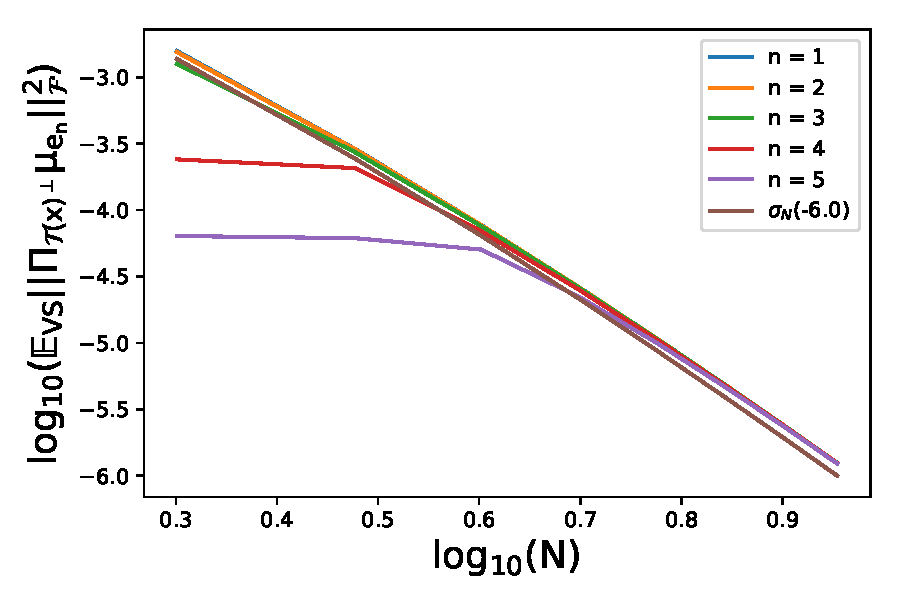
\includegraphics[width= 0.3\textwidth]{figures/EX_VS_err_n_s_3.pdf}\\
% \caption{The expected value of the $n$-th leverage score under the distribution of Volume Sampling for $n \in \{1,2,3,4\}$ for $s =3$.}
% \end{figure}
% \begin{figure}[]
%     \centering
% 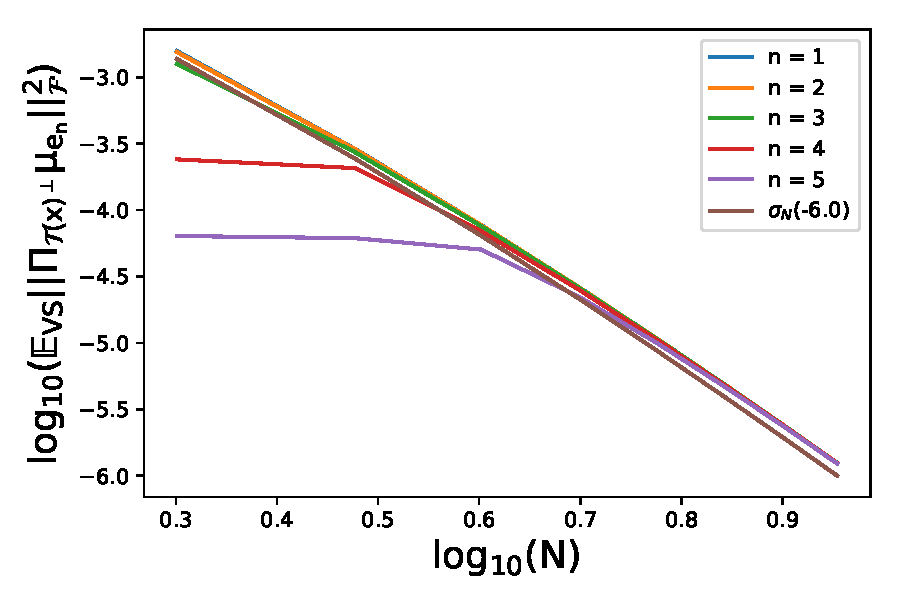
\includegraphics[width= 0.8\textwidth]{figures/EX_VS_err_n_s_3.pdf}\\
% \caption{\label{fig:the_only_one_for_the_moment} The value of $\EX_{\VS} \mathcal{E}(\mu_{e_{m}};\bm{x})^{2}$ for $m \in \{1,2,3,4,5\}$ for the periodic Sobolev space ($s =3,d=1$) compared to the theoretical upper bound (UB) of Theorem~\ref{thm:main_result_1}.}
% \end{figure}


%%%%%%%%%%%%
\subsection{Sketch of the proofs}\label{sec:steps_proof}
 The proof of Theorem~\ref{thm:main_result_1} decomposes into three steps. First, in Section~\ref{sec:decomposition_error}, we write $\mathcal{E}(\mu_{g};\bm{x})^{2}$ as a function of the square of the interpolation errors $\mathcal{E}(\mu_{e_{m}};\bm{x})^{2}$ of the embeddings
$\mu_{e_{m}}$. Then, in Section~\ref{sec:closed_formulas}, we give closed formulas for $\EX_{\VS} \mathcal{E}(\mu_{e_{m}};\bm{x})^{2}$ in terms of the eigenvalues of $\bm{\Sigma}$. Finally, the inequality \eqref{eq:ineq_r_N} is proved using an upper bound on the ratio of symmetric polynomials \citep{GuSi12}. The details are given in Appendix~\ref{app:proof_ineq_r_N}. Finally, The proofs of Theorem~\ref{thm:slow_rates} and Theorem~\ref{thm:EX_VS_integration_error} are straightforward consequences of Theorem~\ref{thm:main_result_1}. The details are given in Appendix~\ref{app:proof_slow_rates} and Appendix~\ref{app:proof_bias}.
%  In particular, the quantities $\epsilon_{m}$ in Theorem~\ref{thm:main_result_1} shall appear to be directly related to the reconstructions of the $e_{m}^{\F}$, where $e_{m}^{\F}$ is the $m$-th $\|.\|_{\F}$-normed eigenfunction of $\bm{\Sigma}$:
% \begin{equation}
% \epsilon_{m} = \EX_{\VS} \|\mu_{e_{m}} - \Pi_{\mathcal{T}(\bm{x})} \mu_{e_{m}}\|_{\F}^{2} =  \sigma_{m} \EX_{\VS} \|e_{m}^{\F} - \Pi_{\mathcal{T}(\bm{x})} e_{m}^{\F}\|_{\F}^{2}.
% \end{equation}

%%%%%%%%%%%%%%
\subsubsection{Decomposing the interpolation error}
\label{sec:decomposition_error}
Let $\bm{x} \in \mathcal{X}^{N}$ such that $\Det \bm{K}(\bm{x}) > 0$. For $m_{1}, m_{2} \in \mathbb{N}^{*}$, let the \emph{cross-leverage score} between $m_{1}$ and $m_{2}$ associated to $\bm{x}$ be
\begin{equation}\label{eq:cross_lvs_def}
\tau_{m_{1},m_{2}}^{\F}(\bm{x}) = e_{m_{1}}^{\F}(\bm{x})^{\Tran} \bm{K}(\bm{x})^{-1} e_{m_{2}}^{\F}(\bm{x}).
\end{equation}
When $m_1=m_2=m$, we speak of the $m$-th leverage score\footnote{Our definition is consistent with the leverage scores used in matrix subsampling  \citep{DrMaMu06}. Loosely speaking, $\tau_{m}^{\F}(\bm{x})$ is the leverage score of the $m$-th column of the semi-infinite matrix  $(e_{n}^{\F}(x_{i}))_{(i,n) \in [N] \times \Ns}$.} associated to $\bm{x}$, and simply write $\tau_{m}^{\F}(\bm{x})$.
% \begin{equation}\label{eq:lvs_def}
% \tau_{m}^{\F}(\bm{x}) = e_{m}^{\F}(\bm{x})^{\Tran} \bm{K}(\bm{x})^{-1} e_{m}^{\F}(\bm{x}), \quad m \in \mathbb{N}^{*}.
% \end{equation}
 % First, the approximation error $\displaystyle \|\mu_{g} - \Pi_{\mathcal{T}(\bm{x})} \mu_{g}\|_{\F}^{2}$ can be decomposed in terms of quantities that quantify the square of the interpolation error of the embeddings $\mu_{e_{m}}$ where $m \in \mathbb{N}^{*}$.
By Lemma~\ref{lemma:lvs_identities},
% \rb{maybe prefix results from the supplementary with an S, and prepare your supplementary paper using zref as we did.}
 the $m$-th leverage score is related to the interpolation error of the $m$-th eigenfunction $e_{m}^{\F}$. Indeed,
\begin{equation}
\|e_{m}^{\F} - \Pi_{\mathcal{T}(\bm{x})} e_{m}^{\F}\|_{\F}^{2} = 1- \tau_{m}^{\F}(\bm{x}) \in [0,1].
\end{equation}
Similarly, for the cross-leverage score,
%between $m_{1}$ and $m_{2}$ is related to the inner product of the reconstructions of the eigenfunctions $e_{m_{1}}^{\F}$ and $e_{m_{2}}^{\F}$:
\begin{equation}
\langle \Pi_{\mathcal{T}(\bm{x})} e_{m_{1}}^{\F}, \Pi_{\mathcal{T}(\bm{x})} e_{m_{2}}^{\F} \rangle_{\F} = \tau_{m_{1},m_{2}}^{\F}(\bm{x}) \in [-1,1].
\end{equation}

For $g \in \Ltwo$, the interpolation error of the embedding $\mu_{g}$ can be expressed using the (cross-)leverage scores.
\begin{lemma}\label{lemma:error_decomposition}
If $\Det \bm{K}(\bm{x}) > 0$, then,
\begin{equation}
\label{e:error_decomposition_in_lemma}
\mathcal{E}(\mu_{g};\bm{x})^{2}  = \sum\limits_{m \in \mathbb{N}^{*}}  g_{m}^{2} \sigma_{n}\bigg(1- \tau_{m}^{\F}(\bm{x})\bigg) - \sum\limits_{m_{1}\neq m_{2} \in \mathbb{N}^{*}}  g_{m_{1}}g_{m_{2}} \sqrt{\sigma_{m_{1}}} \sqrt{\sigma_{m_{2}}} \tau_{m_{1},m_{2}}^{\F}(\bm{x}).
\end{equation}
\end{lemma}
In particular, with probability one, a design sampled from the continuous volume sampling distribution in Definition~\ref{def:VS} satisfies \eqref{e:error_decomposition_in_lemma}. Furthermore, we shall see that the expected value of the (cross-) leverage scores has a simple expression.


%%%%%%%%%%%%%%
\subsubsection{Explicit formulas for expected leverage scores}
\label{sec:closed_formulas}
Proposition~\ref{prop:EX_VS_lvs} expresses expected leverage scores in terms of the spectrum of the integration operator.
\begin{proposition}\label{prop:EX_VS_lvs}
For $m~\in~\mathbb{N}^{*}$,
\begin{equation}\label{eq:lvs_formula}
\EX_{\VS} \tau_{m}^{\F}(\bm{x})  = \frac{1}{\sum\limits_{U \in \: \UN} \prod\limits_{u \in U}\sigma_{u}}  \sum\limits_{\substack{U \in \: \UN \\ m \in U}} \prod\limits_{u \in U}\sigma_{u}.
\end{equation}
Moreover, for $m_{1},m_{2} \in \mathbb{N}^{*}$ such that $m_{1} \neq m_{2}$, we have
\begin{equation}\label{eq:cross_lvs_zero}
\EX_{\VS} \tau_{m_{1},m_{2}}^{\F}(\bm{x}) = 0.
\end{equation}
\end{proposition}

In Appendix~\ref{app:proof_main_result_1}, we combine Lemma~\ref{lemma:error_decomposition} with Proposition~\ref{prop:EX_VS_lvs}. This concludes the proof of Theorem~\ref{thm:main_result_1} by Beppo Levi's monotone convergence theorem.

% following corollary.
% \begin{corollary}\label{cor:EX_VS_mu_g}
% We have
% \begin{equation}
% \EX_{\VS} \|\mu_{g} - \Pi_{\mathcal{T}(\bm{x})} \mu_{g}\|_{\F}^{2}  = \sum\limits_{m \in \mathbb{N}^{*}} g_{m}^{2} \epsilon_{m}.
% \end{equation}
% \end{corollary}

It remains to prove Proposition~\ref{prop:EX_VS_lvs}. Again, we proceed in two steps. First, our Proposition~\ref{thm:EX_lvs_phi} yields a characterization of $ \EX_{\VS}\tau_{m}^{\F}(\bm{x})$ and $\EX_{\VS}\tau_{m_{1},m_{2}}^{\F}(\bm{x})$ in terms of the spectrum of three perturbed versions of the integration operator $\bm{\Sigma}$. Second, we give explicit forms of these spectra in Proposition~\ref{prop:perturbed_kernels_spectrum} below. The idea is to express $\EX_{\VS} \tau_{m}(\bm{x})^{\F}$ as the normalization constant \eqref{eq:normalization_constant_VS} of a perturbation of the kernel $k$.
% \rb{Not sure where this fits in the narrative} For this purpose, we use the Jacobi identity
% \begin{align*}
%   \Det & \bm{K}(\bm{x}) \tau_{m}^{\F}(\bm{x})~=\\
%   & \partial_{t}~\Det~\bigg(~\bm{K}(\bm{x})~+~t e_{m}^{\F}(\bm{x})~e_{m}^{\F}(\bm{x})^{\Tran} \bigg) \bigg|_{t =0^{+}},
% \end{align*}
% see \citep{MaNe19}.
The same goes for $\EX_{\VS} \tau_{m_{1},m_{2}}^{\F}(\bm{x})$.

Let $t\in\mathbb{R}_{+}$ and $\bm{\Sigma}_{t}$, $\bm{\Sigma}_{t}^{+}$ and $\bm{\Sigma}_{t}^{-}$ be the integration operators\footnote{We drop from the notation the dependencies on $m,m_{1}$ and $m_{2}$ for simplicity.} on $\Ltwo$, respectively associated with the kernels
\begin{equation}\label{eq:k_t}
k_{t}(x,y) = k(x,y) + t e_{m}^{\F}(x) e_{m}^{\F}(y),
\end{equation}
\begin{equation}\label{eq:k_t_plus}
k_{t}^{+}(x,y) = k(x,y)
+ t \left( e_{m_{1}}^{\F}(x) + e_{m_{2}}^{\F}(x) \right) \left( e_{m_{1}}^{\F}(y) + e_{m_{2}}^{\F}(y) \right),
\end{equation}
\begin{equation}\label{eq:k_t_minus}
k_{t}^{-}(x,y) = k(x,y) + t \left( e_{m_{1}}^{\F}(x) - e_{m_{2}}^{\F}(x) \right) \left( e_{m_{1}}^{\F}(y) - e_{m_{2}}^{\F}(y) \right).
\end{equation}
By Assumption~\ref{hyp:integrable_diagonal}, and by the fact that $(e_{m})_{m \in \Ns}$ is an orthonormal basis of $\Ltwo$, all three kernels also have integrable diagonals (see Assumption~\ref{hyp:integrable_diagonal}).
% that is,
% \begin{equation}
% \int_{\X} k_{t}(x,x) \mathrm{d}\omega(x) < +\infty, \: \int_{\X} k_{t}^{+}(x,x) \mathrm{d}\omega(x) < +\infty,\text{  and  } \: \: \int_{\X} k_{t}^{-}(x,x) \mathrm{d}\omega(x) < +\infty.
% \end{equation}
In particular, they define RKHSs that can be embedded in $\Ltwo$. Moreover, recalling the definition \eqref{eq:normalization_constant_VS} of the normalization constant $Z_{N}$ of volume sampling, the following quantities are finite
\begin{align}
\phi_{m}(t) = & Z_{N}(k_{t}) , \quad\phi_{m_{1},m_{2}}^{+}(t) = Z_{N}(k_{t}^{+}),&\text{ and }\quad \phi_{m_{1},m_{2}}^{-}(t) = Z_{N}(k_{t}^{-}).
\end{align}
Remember that by Proposition~\ref{prop:VS_decomposition},
\begin{equation}\label{eq:Z_kt}
\phi_{m}(t) = N! \sum\limits_{U \in \: \UN} \prod\limits_{u \in \: U} \tilde{\sigma}_{u}(t),
\end{equation}
where $\displaystyle \{\tilde{\sigma}_{u}(t), \: u \in \Ns\}$ is the set of eigenvalues\footnote{For a given value of $t$, the eigenvalues $\tilde{\sigma}_{u}(t)$ are not necessarily decreasing in $u$. We give explicit formulas for these eigenvalues in Proposition~\ref{prop:perturbed_kernels_spectrum}, and the order satisfied for $t=0$ is not necessarily preserved for $t>0$. This does not change anything to the argument since these eigenvalues only appear in quantities such as $\phi_{m}(t)$ which are invariant under permutation of the eigenvalues.} of $\bm{\Sigma}_{t}$. Similar identities are valid for $\phi_{m_{1},m_{2}}^{+}(t)$ and $\phi_{m_{1},m_{2}}^{-}(t)$ with the eigenvalues of $\bm{\Sigma}_{t}^{+}$ and $\bm{\Sigma}_{t}^{-}$ respectively.

\begin{proposition}\label{thm:EX_lvs_phi}
The functions $\phi_m$, $\phi_{m_1,m_2}^{+}$ and $\phi_{m_1,m_2}^{-}$ are right differentiable in zero. Furthermore,
\begin{equation}\label{eq:EX_lvs_n_delta_phi_n}
\EX_{\VS} \tau_{m}^{\F}(\bm{x})  = \frac{1}{Z_{N}(k)}  \frac{\partial \phi_{m}}{ \partial t }\bigg|_{t = 0^{+}},
\end{equation}
and
\begin{equation}\label{eq:EX_VS_cross_lvs_formula}
\EX_{\VS} \tau_{m_{1},m_{2}}^{\F}(\bm{x}) = \frac{1}{4Z_{N}(k)} \bigg(\frac{\partial \phi_{m_{1},m_{2}}^{+}}{ \partial t } - \frac{\partial \phi_{m_{1},m_{2}}^{-}}{ \partial t }\bigg)\bigg|_{t = 0^{+}}.
\end{equation}
\end{proposition}
 The details of the proof are postponed to Appendix~\ref{app:proof_EX_lvs_phi}. We complete this proposition with a description of the spectrum of the operators $\bm{\Sigma}_{t}$, $\bm{\Sigma}_{t}^{+}$ and $\bm{\Sigma}_{t}^{-}$ using the spectrum of $\bm{\Sigma}$.
\begin{proposition}\label{prop:perturbed_kernels_spectrum}
The eigenvalues of $\bm{\Sigma}_{t}$ write
\begin{equation}
\tilde{\sigma}_{u}(t) =  \left\{
    \begin{array}{ll}
        \sigma_{u} & \mbox{if} \: u \neq m, \\
        (1 + t)\sigma_{u} & \mbox{if}\: u = m.
    \end{array}
\right.
\end{equation}
% and
% \begin{equation}
% \tilde{\sigma}_{u}^{\substack{+\\-}}(t) =  \left\{
%     \begin{array}{ll}
%         \sigma_{u} & \mbox{if} \: u \notin \{m_{1},m_{2}\}, \\
%         (1+t)\frac{\sigma_{m_{1}}+ \sigma_{m_{2}}}{2} + \frac{1}{2} \sqrt{(1+t)^{2}(\sigma_{m_{1}}-\sigma_{m_{2}})^{2}+4 \sigma_{m_{1}}\sigma_{m_{2}}t^{2}} & \mbox{if}\: u = m_{1},\\
%         (1+t)\frac{\sigma_{m_{1}}+ \sigma_{m_{2}}}{2} - \frac{1}{2} \sqrt{(1+t)^{2}(\sigma_{m_{1}}-\sigma_{m_{2}})^{2}+4 \sigma_{m_{1}}\sigma_{m_{2}}t^{2}} & \mbox{if}\: u = m_{2}.
%     \end{array}
% \right.
% \end{equation}
Moreover, the eigenvalues of $\bm{\Sigma}_{t}^{+}$ and $\bm{\Sigma}_{t}^{-}$ satisfy
\begin{equation}\label{eq:equality_positive_negative_spectrum}
\{\tilde{\sigma}_{u}^{+}(t), \: u \in \Ns \} = \{\tilde{\sigma}_{u}^{-}(t), \: u \in \Ns \}.
\end{equation}
\end{proposition}
The proof is based on the observation that the perturbations in \eqref{eq:k_t}, \eqref{eq:k_t_plus}, and \eqref{eq:k_t_minus} only affect a principal subspace of dimension $1$ or $2$; see Appendix~\ref{app:proof_perturbed_kernels_spectrum}.

Combining the characterization of $\EX_{\VS} \tau_{m}^{\F}(\bm{x})$ and $\EX_{\VS} \tau_{m_{1},m_{2}}^{\F}(\bm{x})$ given in Proposition~\ref{thm:EX_lvs_phi}, and Proposition~\ref{prop:perturbed_kernels_spectrum}, we prove Proposition~\ref{prop:EX_VS_lvs}; see details in Appendix~\ref{sec:proof_EX_VS_lvs}.
% This completes the proof of Theorem~\ref{thm:main_result_1}.


%%%%Here%%%%






\clearpage

\section{Interpolation problems in signal processing}

\section{The Richest Hermite Kernel and integration problems in $\mathbb{R}^{d}$}

\section{Future work and conclusion}

\bibliography{bibliography}

\appendix

\section{Details about the simulations of Chapter~\ref{chapter:cssp} }
\section{Proofs of the main results appearing in Chapter~\ref{chapter:cssp} }

%\printbibliography
\end{document}
